\documentclass[twoside]{book}

% Packages required by doxygen
\usepackage{fixltx2e}
\usepackage{calc}
\usepackage{doxygen}
\usepackage[export]{adjustbox} % also loads graphicx
\usepackage{graphicx}
\usepackage[utf8]{inputenc}
\usepackage{makeidx}
\usepackage{multicol}
\usepackage{multirow}
\PassOptionsToPackage{warn}{textcomp}
\usepackage{textcomp}
\usepackage[nointegrals]{wasysym}
\usepackage[table]{xcolor}

% Font selection
\usepackage[T1]{fontenc}
\usepackage[scaled=.90]{helvet}
\usepackage{courier}
\usepackage{amssymb}
\usepackage{sectsty}
\renewcommand{\familydefault}{\sfdefault}
\allsectionsfont{%
  \fontseries{bc}\selectfont%
  \color{darkgray}%
}
\renewcommand{\DoxyLabelFont}{%
  \fontseries{bc}\selectfont%
  \color{darkgray}%
}
\newcommand{\+}{\discretionary{\mbox{\scriptsize$\hookleftarrow$}}{}{}}

% Page & text layout
\usepackage{geometry}
\geometry{%
  a4paper,%
  top=2.5cm,%
  bottom=2.5cm,%
  left=2.5cm,%
  right=2.5cm%
}
\tolerance=750
\hfuzz=15pt
\hbadness=750
\setlength{\emergencystretch}{15pt}
\setlength{\parindent}{0cm}
\setlength{\parskip}{3ex plus 2ex minus 2ex}
\makeatletter
\renewcommand{\paragraph}{%
  \@startsection{paragraph}{4}{0ex}{-1.0ex}{1.0ex}{%
    \normalfont\normalsize\bfseries\SS@parafont%
  }%
}
\renewcommand{\subparagraph}{%
  \@startsection{subparagraph}{5}{0ex}{-1.0ex}{1.0ex}{%
    \normalfont\normalsize\bfseries\SS@subparafont%
  }%
}
\makeatother

% Headers & footers
\usepackage{fancyhdr}
\pagestyle{fancyplain}
\fancyhead[LE]{\fancyplain{}{\bfseries\thepage}}
\fancyhead[CE]{\fancyplain{}{}}
\fancyhead[RE]{\fancyplain{}{\bfseries\leftmark}}
\fancyhead[LO]{\fancyplain{}{\bfseries\rightmark}}
\fancyhead[CO]{\fancyplain{}{}}
\fancyhead[RO]{\fancyplain{}{\bfseries\thepage}}
\fancyfoot[LE]{\fancyplain{}{}}
\fancyfoot[CE]{\fancyplain{}{}}
\fancyfoot[RE]{\fancyplain{}{\bfseries\scriptsize Generated by Doxygen }}
\fancyfoot[LO]{\fancyplain{}{\bfseries\scriptsize Generated by Doxygen }}
\fancyfoot[CO]{\fancyplain{}{}}
\fancyfoot[RO]{\fancyplain{}{}}
\renewcommand{\footrulewidth}{0.4pt}
\renewcommand{\chaptermark}[1]{%
  \markboth{#1}{}%
}
\renewcommand{\sectionmark}[1]{%
  \markright{\thesection\ #1}%
}

% Indices & bibliography
\usepackage{natbib}
\usepackage[titles]{tocloft}
\setcounter{tocdepth}{3}
\setcounter{secnumdepth}{5}
\makeindex

% Hyperlinks (required, but should be loaded last)
\usepackage{ifpdf}
\ifpdf
  \usepackage[pdftex,pagebackref=true]{hyperref}
\else
  \usepackage[ps2pdf,pagebackref=true]{hyperref}
\fi
\hypersetup{%
  colorlinks=true,%
  linkcolor=blue,%
  citecolor=blue,%
  unicode%
}

% Custom commands
\newcommand{\clearemptydoublepage}{%
  \newpage{\pagestyle{empty}\cleardoublepage}%
}

\usepackage{caption}
\captionsetup{labelsep=space,justification=centering,font={bf},singlelinecheck=off,skip=4pt,position=top}

%===== C O N T E N T S =====

\begin{document}

% Titlepage & ToC
\hypersetup{pageanchor=false,
             bookmarksnumbered=true,
             pdfencoding=unicode
            }
\pagenumbering{alph}
\begin{titlepage}
\vspace*{7cm}
\begin{center}%
{\Large Jeu de Go \\[1ex]\large 1.\+4 }\\
\vspace*{1cm}
{\large Generated by Doxygen 1.8.13}\\
\end{center}
\end{titlepage}
\clearemptydoublepage
\pagenumbering{roman}
\tableofcontents
\clearemptydoublepage
\pagenumbering{arabic}
\hypersetup{pageanchor=true}

%--- Begin generated contents ---
\chapter{Hierarchical Index}
\section{Class Hierarchy}
This inheritance list is sorted roughly, but not completely, alphabetically\+:\begin{DoxyCompactList}
\item \contentsline{section}{Arbre}{\pageref{class_arbre}}{}
\item Clock\begin{DoxyCompactList}
\item \contentsline{section}{Timer}{\pageref{class_timer}}{}
\end{DoxyCompactList}
\item Drawable\begin{DoxyCompactList}
\item \contentsline{section}{Board}{\pageref{class_board}}{}
\item \contentsline{section}{Choice}{\pageref{class_choice}}{}
\begin{DoxyCompactList}
\item \contentsline{section}{Choice\+\_\+miniature}{\pageref{class_choice__miniature}}{}
\item \contentsline{section}{Choice\+\_\+\+Simple}{\pageref{class_choice___simple}}{}
\end{DoxyCompactList}
\item \contentsline{section}{Infos}{\pageref{class_infos}}{}
\item \contentsline{section}{Screen}{\pageref{class_screen}}{}
\begin{DoxyCompactList}
\item \contentsline{section}{Game\+\_\+window}{\pageref{class_game__window}}{}
\item \contentsline{section}{Menu}{\pageref{class_menu}}{}
\begin{DoxyCompactList}
\item \contentsline{section}{Menu\+\_\+\+Miniature}{\pageref{class_menu___miniature}}{}
\item \contentsline{section}{Menu\+\_\+simple}{\pageref{class_menu__simple}}{}
\end{DoxyCompactList}
\end{DoxyCompactList}
\item \contentsline{section}{Square}{\pageref{class_square}}{}
\end{DoxyCompactList}
\item \contentsline{section}{Etat}{\pageref{class_etat}}{}
\item \contentsline{section}{Goban}{\pageref{class_goban}}{}
\item list\begin{DoxyCompactList}
\item \contentsline{section}{History}{\pageref{class_history}}{}
\end{DoxyCompactList}
\item Text\begin{DoxyCompactList}
\item \contentsline{section}{Timer}{\pageref{class_timer}}{}
\end{DoxyCompactList}
\item vector\begin{DoxyCompactList}
\item \contentsline{section}{Groupe}{\pageref{class_groupe}}{}
\end{DoxyCompactList}
\end{DoxyCompactList}

\chapter{Class Index}
\section{Class List}
Here are the classes, structs, unions and interfaces with brief descriptions\+:\begin{DoxyCompactList}
\item\contentsline{section}{\hyperlink{class_arbre}{Arbre} }{\pageref{class_arbre}}{}
\item\contentsline{section}{\hyperlink{class_board}{Board} }{\pageref{class_board}}{}
\item\contentsline{section}{\hyperlink{class_choice}{Choice} }{\pageref{class_choice}}{}
\item\contentsline{section}{\hyperlink{class_choice__miniature}{Choice\+\_\+miniature} }{\pageref{class_choice__miniature}}{}
\item\contentsline{section}{\hyperlink{class_choice___simple}{Choice\+\_\+\+Simple} }{\pageref{class_choice___simple}}{}
\item\contentsline{section}{\hyperlink{class_etat}{Etat} }{\pageref{class_etat}}{}
\item\contentsline{section}{\hyperlink{class_game__window}{Game\+\_\+window} }{\pageref{class_game__window}}{}
\item\contentsline{section}{\hyperlink{class_goban}{Goban} }{\pageref{class_goban}}{}
\item\contentsline{section}{\hyperlink{class_groupe}{Groupe} }{\pageref{class_groupe}}{}
\item\contentsline{section}{\hyperlink{class_history}{History} }{\pageref{class_history}}{}
\item\contentsline{section}{\hyperlink{class_infos}{Infos} }{\pageref{class_infos}}{}
\item\contentsline{section}{\hyperlink{class_menu}{Menu} }{\pageref{class_menu}}{}
\item\contentsline{section}{\hyperlink{class_menu___miniature}{Menu\+\_\+\+Miniature} }{\pageref{class_menu___miniature}}{}
\item\contentsline{section}{\hyperlink{class_menu__simple}{Menu\+\_\+simple} }{\pageref{class_menu__simple}}{}
\item\contentsline{section}{\hyperlink{class_screen}{Screen} }{\pageref{class_screen}}{}
\item\contentsline{section}{\hyperlink{class_square}{Square} }{\pageref{class_square}}{}
\item\contentsline{section}{\hyperlink{class_timer}{Timer} }{\pageref{class_timer}}{}
\end{DoxyCompactList}

\chapter{File Index}
\section{File List}
Here is a list of all files with brief descriptions\+:\begin{DoxyCompactList}
\item\contentsline{section}{D\+:/\+Users/\+Victor/\+One\+Drive/\+Documents/\+Visual Studio 2017/\+Projects/\+Jeu\+\_\+de\+\_\+\+Go/\+Jeu\+\_\+de\+\_\+\+Go/\+Sources/\+Engine/\hyperlink{_arbre_8cpp}{Arbre.\+cpp} }{\pageref{_arbre_8cpp}}{}
\item\contentsline{section}{D\+:/\+Users/\+Victor/\+One\+Drive/\+Documents/\+Visual Studio 2017/\+Projects/\+Jeu\+\_\+de\+\_\+\+Go/\+Jeu\+\_\+de\+\_\+\+Go/\+Sources/\+Engine/\hyperlink{_arbre_8h}{Arbre.\+h} }{\pageref{_arbre_8h}}{}
\item\contentsline{section}{D\+:/\+Users/\+Victor/\+One\+Drive/\+Documents/\+Visual Studio 2017/\+Projects/\+Jeu\+\_\+de\+\_\+\+Go/\+Jeu\+\_\+de\+\_\+\+Go/\+Sources/\+Engine/\hyperlink{_etat_8cpp}{Etat.\+cpp} }{\pageref{_etat_8cpp}}{}
\item\contentsline{section}{D\+:/\+Users/\+Victor/\+One\+Drive/\+Documents/\+Visual Studio 2017/\+Projects/\+Jeu\+\_\+de\+\_\+\+Go/\+Jeu\+\_\+de\+\_\+\+Go/\+Sources/\+Engine/\hyperlink{_etat_8h}{Etat.\+h} }{\pageref{_etat_8h}}{}
\item\contentsline{section}{D\+:/\+Users/\+Victor/\+One\+Drive/\+Documents/\+Visual Studio 2017/\+Projects/\+Jeu\+\_\+de\+\_\+\+Go/\+Jeu\+\_\+de\+\_\+\+Go/\+Sources/\+Engine/\hyperlink{_goban_8cpp}{Goban.\+cpp} }{\pageref{_goban_8cpp}}{}
\item\contentsline{section}{D\+:/\+Users/\+Victor/\+One\+Drive/\+Documents/\+Visual Studio 2017/\+Projects/\+Jeu\+\_\+de\+\_\+\+Go/\+Jeu\+\_\+de\+\_\+\+Go/\+Sources/\+Engine/\hyperlink{_goban_8h}{Goban.\+h} }{\pageref{_goban_8h}}{}
\item\contentsline{section}{D\+:/\+Users/\+Victor/\+One\+Drive/\+Documents/\+Visual Studio 2017/\+Projects/\+Jeu\+\_\+de\+\_\+\+Go/\+Jeu\+\_\+de\+\_\+\+Go/\+Sources/\+Engine/\hyperlink{_groupe_8cpp}{Groupe.\+cpp} }{\pageref{_groupe_8cpp}}{}
\item\contentsline{section}{D\+:/\+Users/\+Victor/\+One\+Drive/\+Documents/\+Visual Studio 2017/\+Projects/\+Jeu\+\_\+de\+\_\+\+Go/\+Jeu\+\_\+de\+\_\+\+Go/\+Sources/\+Engine/\hyperlink{_groupe_8h}{Groupe.\+h} }{\pageref{_groupe_8h}}{}
\item\contentsline{section}{D\+:/\+Users/\+Victor/\+One\+Drive/\+Documents/\+Visual Studio 2017/\+Projects/\+Jeu\+\_\+de\+\_\+\+Go/\+Jeu\+\_\+de\+\_\+\+Go/\+Sources/\+Engine/\hyperlink{_history_8cpp}{History.\+cpp} }{\pageref{_history_8cpp}}{}
\item\contentsline{section}{D\+:/\+Users/\+Victor/\+One\+Drive/\+Documents/\+Visual Studio 2017/\+Projects/\+Jeu\+\_\+de\+\_\+\+Go/\+Jeu\+\_\+de\+\_\+\+Go/\+Sources/\+Engine/\hyperlink{_history_8h}{History.\+h} }{\pageref{_history_8h}}{}
\item\contentsline{section}{D\+:/\+Users/\+Victor/\+One\+Drive/\+Documents/\+Visual Studio 2017/\+Projects/\+Jeu\+\_\+de\+\_\+\+Go/\+Jeu\+\_\+de\+\_\+\+Go/\+Sources/\+Engine/\hyperlink{_parser_8cpp}{Parser.\+cpp} }{\pageref{_parser_8cpp}}{}
\item\contentsline{section}{D\+:/\+Users/\+Victor/\+One\+Drive/\+Documents/\+Visual Studio 2017/\+Projects/\+Jeu\+\_\+de\+\_\+\+Go/\+Jeu\+\_\+de\+\_\+\+Go/\+Sources/\+Engine/\hyperlink{_parser_8h}{Parser.\+h} }{\pageref{_parser_8h}}{}
\item\contentsline{section}{D\+:/\+Users/\+Victor/\+One\+Drive/\+Documents/\+Visual Studio 2017/\+Projects/\+Jeu\+\_\+de\+\_\+\+Go/\+Jeu\+\_\+de\+\_\+\+Go/\+Sources/\+Graphics/\hyperlink{_choice_8cpp}{Choice.\+cpp} }{\pageref{_choice_8cpp}}{}
\item\contentsline{section}{D\+:/\+Users/\+Victor/\+One\+Drive/\+Documents/\+Visual Studio 2017/\+Projects/\+Jeu\+\_\+de\+\_\+\+Go/\+Jeu\+\_\+de\+\_\+\+Go/\+Sources/\+Graphics/\hyperlink{_choice_8h}{Choice.\+h} }{\pageref{_choice_8h}}{}
\item\contentsline{section}{D\+:/\+Users/\+Victor/\+One\+Drive/\+Documents/\+Visual Studio 2017/\+Projects/\+Jeu\+\_\+de\+\_\+\+Go/\+Jeu\+\_\+de\+\_\+\+Go/\+Sources/\+Graphics/\hyperlink{_choice__miniature_8cpp}{Choice\+\_\+miniature.\+cpp} }{\pageref{_choice__miniature_8cpp}}{}
\item\contentsline{section}{D\+:/\+Users/\+Victor/\+One\+Drive/\+Documents/\+Visual Studio 2017/\+Projects/\+Jeu\+\_\+de\+\_\+\+Go/\+Jeu\+\_\+de\+\_\+\+Go/\+Sources/\+Graphics/\hyperlink{_choice__miniature_8h}{Choice\+\_\+miniature.\+h} }{\pageref{_choice__miniature_8h}}{}
\item\contentsline{section}{D\+:/\+Users/\+Victor/\+One\+Drive/\+Documents/\+Visual Studio 2017/\+Projects/\+Jeu\+\_\+de\+\_\+\+Go/\+Jeu\+\_\+de\+\_\+\+Go/\+Sources/\+Graphics/\hyperlink{_choice___simple_8cpp}{Choice\+\_\+\+Simple.\+cpp} }{\pageref{_choice___simple_8cpp}}{}
\item\contentsline{section}{D\+:/\+Users/\+Victor/\+One\+Drive/\+Documents/\+Visual Studio 2017/\+Projects/\+Jeu\+\_\+de\+\_\+\+Go/\+Jeu\+\_\+de\+\_\+\+Go/\+Sources/\+Graphics/\hyperlink{_choice___simple_8h}{Choice\+\_\+\+Simple.\+h} }{\pageref{_choice___simple_8h}}{}
\item\contentsline{section}{D\+:/\+Users/\+Victor/\+One\+Drive/\+Documents/\+Visual Studio 2017/\+Projects/\+Jeu\+\_\+de\+\_\+\+Go/\+Jeu\+\_\+de\+\_\+\+Go/\+Sources/\+Graphics/\hyperlink{_globals_8h}{Globals.\+h} }{\pageref{_globals_8h}}{}
\item\contentsline{section}{D\+:/\+Users/\+Victor/\+One\+Drive/\+Documents/\+Visual Studio 2017/\+Projects/\+Jeu\+\_\+de\+\_\+\+Go/\+Jeu\+\_\+de\+\_\+\+Go/\+Sources/\+Graphics/\hyperlink{_main_8cpp}{Main.\+cpp} }{\pageref{_main_8cpp}}{}
\item\contentsline{section}{D\+:/\+Users/\+Victor/\+One\+Drive/\+Documents/\+Visual Studio 2017/\+Projects/\+Jeu\+\_\+de\+\_\+\+Go/\+Jeu\+\_\+de\+\_\+\+Go/\+Sources/\+Graphics/\hyperlink{_menu_8cpp}{Menu.\+cpp} }{\pageref{_menu_8cpp}}{}
\item\contentsline{section}{D\+:/\+Users/\+Victor/\+One\+Drive/\+Documents/\+Visual Studio 2017/\+Projects/\+Jeu\+\_\+de\+\_\+\+Go/\+Jeu\+\_\+de\+\_\+\+Go/\+Sources/\+Graphics/\hyperlink{_menu_8h}{Menu.\+h} }{\pageref{_menu_8h}}{}
\item\contentsline{section}{D\+:/\+Users/\+Victor/\+One\+Drive/\+Documents/\+Visual Studio 2017/\+Projects/\+Jeu\+\_\+de\+\_\+\+Go/\+Jeu\+\_\+de\+\_\+\+Go/\+Sources/\+Graphics/\hyperlink{_menu___miniature_8cpp}{Menu\+\_\+\+Miniature.\+cpp} }{\pageref{_menu___miniature_8cpp}}{}
\item\contentsline{section}{D\+:/\+Users/\+Victor/\+One\+Drive/\+Documents/\+Visual Studio 2017/\+Projects/\+Jeu\+\_\+de\+\_\+\+Go/\+Jeu\+\_\+de\+\_\+\+Go/\+Sources/\+Graphics/\hyperlink{_menu___miniature_8h}{Menu\+\_\+\+Miniature.\+h} }{\pageref{_menu___miniature_8h}}{}
\item\contentsline{section}{D\+:/\+Users/\+Victor/\+One\+Drive/\+Documents/\+Visual Studio 2017/\+Projects/\+Jeu\+\_\+de\+\_\+\+Go/\+Jeu\+\_\+de\+\_\+\+Go/\+Sources/\+Graphics/\hyperlink{_menu__simple_8cpp}{Menu\+\_\+simple.\+cpp} }{\pageref{_menu__simple_8cpp}}{}
\item\contentsline{section}{D\+:/\+Users/\+Victor/\+One\+Drive/\+Documents/\+Visual Studio 2017/\+Projects/\+Jeu\+\_\+de\+\_\+\+Go/\+Jeu\+\_\+de\+\_\+\+Go/\+Sources/\+Graphics/\hyperlink{_menu__simple_8h}{Menu\+\_\+simple.\+h} }{\pageref{_menu__simple_8h}}{}
\item\contentsline{section}{D\+:/\+Users/\+Victor/\+One\+Drive/\+Documents/\+Visual Studio 2017/\+Projects/\+Jeu\+\_\+de\+\_\+\+Go/\+Jeu\+\_\+de\+\_\+\+Go/\+Sources/\+Graphics/\hyperlink{_screen_8h}{Screen.\+h} }{\pageref{_screen_8h}}{}
\item\contentsline{section}{D\+:/\+Users/\+Victor/\+One\+Drive/\+Documents/\+Visual Studio 2017/\+Projects/\+Jeu\+\_\+de\+\_\+\+Go/\+Jeu\+\_\+de\+\_\+\+Go/\+Sources/\+Graphics/\hyperlink{_screens_8h}{Screens.\+h} }{\pageref{_screens_8h}}{}
\item\contentsline{section}{D\+:/\+Users/\+Victor/\+One\+Drive/\+Documents/\+Visual Studio 2017/\+Projects/\+Jeu\+\_\+de\+\_\+\+Go/\+Jeu\+\_\+de\+\_\+\+Go/\+Sources/\+Graphics/\+Game/\hyperlink{_board_8cpp}{Board.\+cpp} }{\pageref{_board_8cpp}}{}
\item\contentsline{section}{D\+:/\+Users/\+Victor/\+One\+Drive/\+Documents/\+Visual Studio 2017/\+Projects/\+Jeu\+\_\+de\+\_\+\+Go/\+Jeu\+\_\+de\+\_\+\+Go/\+Sources/\+Graphics/\+Game/\hyperlink{_board_8h}{Board.\+h} }{\pageref{_board_8h}}{}
\item\contentsline{section}{D\+:/\+Users/\+Victor/\+One\+Drive/\+Documents/\+Visual Studio 2017/\+Projects/\+Jeu\+\_\+de\+\_\+\+Go/\+Jeu\+\_\+de\+\_\+\+Go/\+Sources/\+Graphics/\+Game/\hyperlink{_game__window_8cpp}{Game\+\_\+window.\+cpp} }{\pageref{_game__window_8cpp}}{}
\item\contentsline{section}{D\+:/\+Users/\+Victor/\+One\+Drive/\+Documents/\+Visual Studio 2017/\+Projects/\+Jeu\+\_\+de\+\_\+\+Go/\+Jeu\+\_\+de\+\_\+\+Go/\+Sources/\+Graphics/\+Game/\hyperlink{_game__window_8h}{Game\+\_\+window.\+h} }{\pageref{_game__window_8h}}{}
\item\contentsline{section}{D\+:/\+Users/\+Victor/\+One\+Drive/\+Documents/\+Visual Studio 2017/\+Projects/\+Jeu\+\_\+de\+\_\+\+Go/\+Jeu\+\_\+de\+\_\+\+Go/\+Sources/\+Graphics/\+Game/\hyperlink{_infos_8cpp}{Infos.\+cpp} }{\pageref{_infos_8cpp}}{}
\item\contentsline{section}{D\+:/\+Users/\+Victor/\+One\+Drive/\+Documents/\+Visual Studio 2017/\+Projects/\+Jeu\+\_\+de\+\_\+\+Go/\+Jeu\+\_\+de\+\_\+\+Go/\+Sources/\+Graphics/\+Game/\hyperlink{_infos_8h}{Infos.\+h} }{\pageref{_infos_8h}}{}
\item\contentsline{section}{D\+:/\+Users/\+Victor/\+One\+Drive/\+Documents/\+Visual Studio 2017/\+Projects/\+Jeu\+\_\+de\+\_\+\+Go/\+Jeu\+\_\+de\+\_\+\+Go/\+Sources/\+Graphics/\+Game/\hyperlink{_square_8cpp}{Square.\+cpp} }{\pageref{_square_8cpp}}{}
\item\contentsline{section}{D\+:/\+Users/\+Victor/\+One\+Drive/\+Documents/\+Visual Studio 2017/\+Projects/\+Jeu\+\_\+de\+\_\+\+Go/\+Jeu\+\_\+de\+\_\+\+Go/\+Sources/\+Graphics/\+Game/\hyperlink{_square_8h}{Square.\+h} }{\pageref{_square_8h}}{}
\item\contentsline{section}{D\+:/\+Users/\+Victor/\+One\+Drive/\+Documents/\+Visual Studio 2017/\+Projects/\+Jeu\+\_\+de\+\_\+\+Go/\+Jeu\+\_\+de\+\_\+\+Go/\+Sources/\+Graphics/\+Game/\hyperlink{_timer_8cpp}{Timer.\+cpp} }{\pageref{_timer_8cpp}}{}
\item\contentsline{section}{D\+:/\+Users/\+Victor/\+One\+Drive/\+Documents/\+Visual Studio 2017/\+Projects/\+Jeu\+\_\+de\+\_\+\+Go/\+Jeu\+\_\+de\+\_\+\+Go/\+Sources/\+Graphics/\+Game/\hyperlink{_timer_8h}{Timer.\+h} }{\pageref{_timer_8h}}{}
\end{DoxyCompactList}

\chapter{Class Documentation}
\hypertarget{class_arbre}{}\section{Arbre Class Reference}
\label{class_arbre}\index{Arbre@{Arbre}}


{\ttfamily \#include $<$Arbre.\+h$>$}



Collaboration diagram for Arbre\+:\nopagebreak
\begin{figure}[H]
\begin{center}
\leavevmode
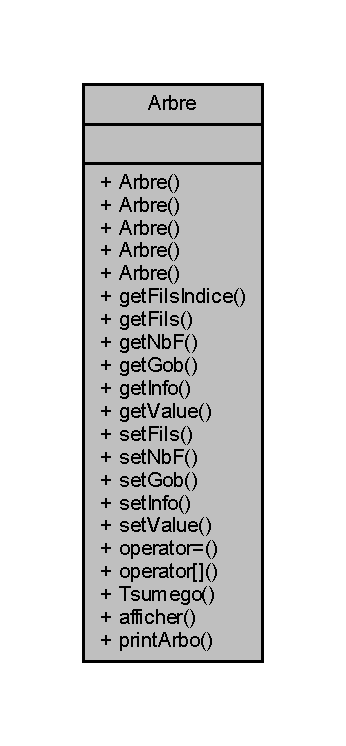
\includegraphics[width=166pt]{class_arbre__coll__graph}
\end{center}
\end{figure}
\subsection*{Public Member Functions}
\begin{DoxyCompactItemize}
\item 
\hyperlink{class_arbre_a761f4a2c6a43f44b38d4ac6fc1cf5cae}{Arbre} ()
\item 
\hyperlink{class_arbre_a3284c47c1ea92a6c5be4a210008dfb4f}{Arbre} (const \hyperlink{class_arbre}{Arbre} \&)
\item 
\hyperlink{class_arbre_ac82e543d8cbf0aced4d741c346f9950d}{Arbre} (\hyperlink{class_goban}{Goban} \&, \hyperlink{class_etat_af3ddb2296ffc379b7f3ad2bf832f294e}{Etat\+::\+V\+AL})
\item 
\hyperlink{class_arbre_acaa1b2ef290ae35e414d6fc5510c9e6e}{Arbre} (\hyperlink{class_goban}{Goban} \&, const size\+\_\+t)
\item 
\hyperlink{class_arbre_a7be58ac146487307f93a5c141f3546df}{Arbre} (\hyperlink{class_goban}{Goban} \&\+\_\+gob, const size\+\_\+t \+\_\+nbF, \hyperlink{class_goban}{Goban} $\ast$\+\_\+fils)
\item 
\hyperlink{class_goban}{Goban} \hyperlink{class_arbre_a46ec1d0b89a9466c87a31e8e43133099}{get\+Fils\+Indice} (const size\+\_\+t) const
\item 
std\+::vector$<$ \hyperlink{class_goban}{Goban} $>$ \hyperlink{class_arbre_ace487e80301c07e6369108bf9a480513}{get\+Fils} () const
\item 
size\+\_\+t \hyperlink{class_arbre_a0aef1f091d76bca13229a21fcd45a076}{get\+NbF} () const
\item 
\hyperlink{class_goban}{Goban} \hyperlink{class_arbre_abb30fa37b209f6e148a5dc29e3a1c00d}{get\+Gob} () const
\item 
bool \hyperlink{class_arbre_afc71a182e86352b06193c2dc746fab79}{get\+Info} () const
\item 
\hyperlink{class_etat_af3ddb2296ffc379b7f3ad2bf832f294e}{Etat\+::\+V\+AL} \hyperlink{class_arbre_aeaa93d0b192e3cce04adb509b6b29c40}{get\+Value} () const
\item 
void \hyperlink{class_arbre_ad7db2ec4bca90d9523c9dab19eadd628}{set\+Fils} (\hyperlink{class_goban}{Goban}, const size\+\_\+t)
\item 
void \hyperlink{class_arbre_acabc45692262e5ca9c2f7b410ddcd373}{set\+NbF} (size\+\_\+t)
\item 
void \hyperlink{class_arbre_a36267e74d40f509fd63b99fe6d8dae0b}{set\+Gob} (\hyperlink{class_goban}{Goban})
\item 
void \hyperlink{class_arbre_a051e5328c63ba7ab6f6359f9f2f77105}{set\+Info} (bool)
\item 
void \hyperlink{class_arbre_a8108ffdff578e323dd9e50cc105a5c04}{set\+Value} (\hyperlink{class_etat_af3ddb2296ffc379b7f3ad2bf832f294e}{Etat\+::\+V\+AL})
\item 
\hyperlink{class_arbre}{Arbre} \hyperlink{class_arbre_a2a919273c1041a7f024f717cdd638632}{operator=} (\hyperlink{class_arbre}{Arbre})
\item 
\hyperlink{class_goban}{Goban} \hyperlink{class_arbre_a8127785309368d2f2cd5a68f913e18cd}{operator\mbox{[}$\,$\mbox{]}} (unsigned short int)
\item 
void \hyperlink{class_arbre_acd12cae4820bb7780a628716a0615d10}{Tsumego} (\hyperlink{class_etat}{Etat} \&)
\item 
void \hyperlink{class_arbre_a970de955ffdbbd5894e0fa0c40c4e69e}{afficher} ()
\item 
void \hyperlink{class_arbre_ac6329911b0037ca669e6ef2e12a178c9}{print\+Arbo} (const \hyperlink{class_arbre}{Arbre} \&)
\end{DoxyCompactItemize}


\subsection{Constructor \& Destructor Documentation}
\mbox{\Hypertarget{class_arbre_a761f4a2c6a43f44b38d4ac6fc1cf5cae}\label{class_arbre_a761f4a2c6a43f44b38d4ac6fc1cf5cae}} 
\index{Arbre@{Arbre}!Arbre@{Arbre}}
\index{Arbre@{Arbre}!Arbre@{Arbre}}
\subsubsection{\texorpdfstring{Arbre()}{Arbre()}\hspace{0.1cm}{\footnotesize\ttfamily [1/5]}}
{\footnotesize\ttfamily Arbre\+::\+Arbre (\begin{DoxyParamCaption}{ }\end{DoxyParamCaption})}

Here is the caller graph for this function\+:\nopagebreak
\begin{figure}[H]
\begin{center}
\leavevmode
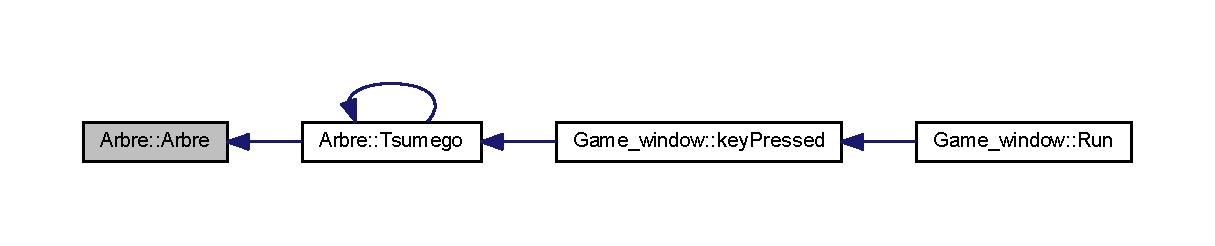
\includegraphics[width=350pt]{class_arbre_a761f4a2c6a43f44b38d4ac6fc1cf5cae_icgraph}
\end{center}
\end{figure}
\mbox{\Hypertarget{class_arbre_a3284c47c1ea92a6c5be4a210008dfb4f}\label{class_arbre_a3284c47c1ea92a6c5be4a210008dfb4f}} 
\index{Arbre@{Arbre}!Arbre@{Arbre}}
\index{Arbre@{Arbre}!Arbre@{Arbre}}
\subsubsection{\texorpdfstring{Arbre()}{Arbre()}\hspace{0.1cm}{\footnotesize\ttfamily [2/5]}}
{\footnotesize\ttfamily Arbre\+::\+Arbre (\begin{DoxyParamCaption}\item[{const \hyperlink{class_arbre}{Arbre} \&}]{a }\end{DoxyParamCaption})}

Here is the call graph for this function\+:\nopagebreak
\begin{figure}[H]
\begin{center}
\leavevmode
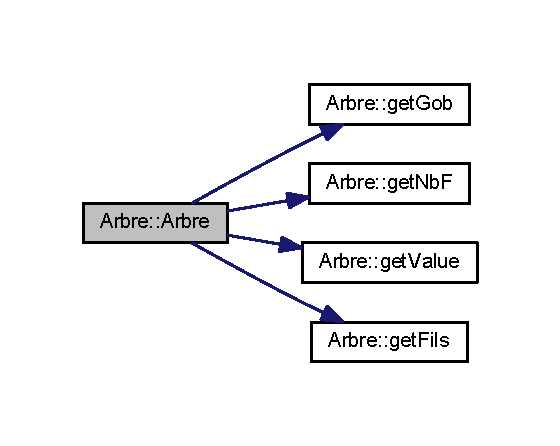
\includegraphics[width=269pt]{class_arbre_a3284c47c1ea92a6c5be4a210008dfb4f_cgraph}
\end{center}
\end{figure}
\mbox{\Hypertarget{class_arbre_ac82e543d8cbf0aced4d741c346f9950d}\label{class_arbre_ac82e543d8cbf0aced4d741c346f9950d}} 
\index{Arbre@{Arbre}!Arbre@{Arbre}}
\index{Arbre@{Arbre}!Arbre@{Arbre}}
\subsubsection{\texorpdfstring{Arbre()}{Arbre()}\hspace{0.1cm}{\footnotesize\ttfamily [3/5]}}
{\footnotesize\ttfamily Arbre\+::\+Arbre (\begin{DoxyParamCaption}\item[{\hyperlink{class_goban}{Goban} \&}]{G,  }\item[{\hyperlink{class_etat_af3ddb2296ffc379b7f3ad2bf832f294e}{Etat\+::\+V\+AL}}]{val }\end{DoxyParamCaption})}

\mbox{\Hypertarget{class_arbre_acaa1b2ef290ae35e414d6fc5510c9e6e}\label{class_arbre_acaa1b2ef290ae35e414d6fc5510c9e6e}} 
\index{Arbre@{Arbre}!Arbre@{Arbre}}
\index{Arbre@{Arbre}!Arbre@{Arbre}}
\subsubsection{\texorpdfstring{Arbre()}{Arbre()}\hspace{0.1cm}{\footnotesize\ttfamily [4/5]}}
{\footnotesize\ttfamily Arbre\+::\+Arbre (\begin{DoxyParamCaption}\item[{\hyperlink{class_goban}{Goban} \&}]{,  }\item[{const size\+\_\+t}]{ }\end{DoxyParamCaption})}

\mbox{\Hypertarget{class_arbre_a7be58ac146487307f93a5c141f3546df}\label{class_arbre_a7be58ac146487307f93a5c141f3546df}} 
\index{Arbre@{Arbre}!Arbre@{Arbre}}
\index{Arbre@{Arbre}!Arbre@{Arbre}}
\subsubsection{\texorpdfstring{Arbre()}{Arbre()}\hspace{0.1cm}{\footnotesize\ttfamily [5/5]}}
{\footnotesize\ttfamily Arbre\+::\+Arbre (\begin{DoxyParamCaption}\item[{\hyperlink{class_goban}{Goban} \&}]{\+\_\+gob,  }\item[{const size\+\_\+t}]{\+\_\+nbF,  }\item[{\hyperlink{class_goban}{Goban} $\ast$}]{\+\_\+fils }\end{DoxyParamCaption})}



\subsection{Member Function Documentation}
\mbox{\Hypertarget{class_arbre_a970de955ffdbbd5894e0fa0c40c4e69e}\label{class_arbre_a970de955ffdbbd5894e0fa0c40c4e69e}} 
\index{Arbre@{Arbre}!afficher@{afficher}}
\index{afficher@{afficher}!Arbre@{Arbre}}
\subsubsection{\texorpdfstring{afficher()}{afficher()}}
{\footnotesize\ttfamily void Arbre\+::afficher (\begin{DoxyParamCaption}{ }\end{DoxyParamCaption})}

Here is the call graph for this function\+:\nopagebreak
\begin{figure}[H]
\begin{center}
\leavevmode
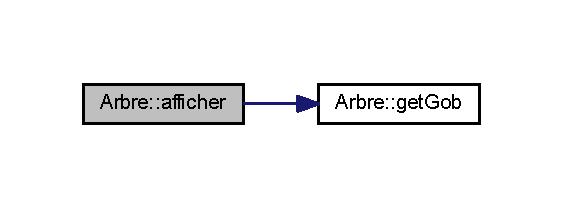
\includegraphics[width=270pt]{class_arbre_a970de955ffdbbd5894e0fa0c40c4e69e_cgraph}
\end{center}
\end{figure}
Here is the caller graph for this function\+:\nopagebreak
\begin{figure}[H]
\begin{center}
\leavevmode
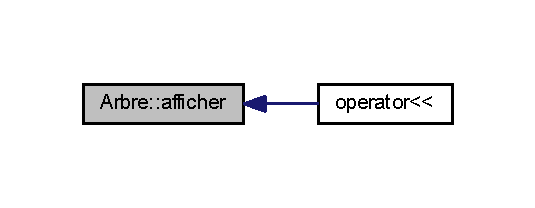
\includegraphics[width=257pt]{class_arbre_a970de955ffdbbd5894e0fa0c40c4e69e_icgraph}
\end{center}
\end{figure}
\mbox{\Hypertarget{class_arbre_ace487e80301c07e6369108bf9a480513}\label{class_arbre_ace487e80301c07e6369108bf9a480513}} 
\index{Arbre@{Arbre}!get\+Fils@{get\+Fils}}
\index{get\+Fils@{get\+Fils}!Arbre@{Arbre}}
\subsubsection{\texorpdfstring{get\+Fils()}{getFils()}}
{\footnotesize\ttfamily std\+::vector$<$ \hyperlink{class_goban}{Goban} $>$ Arbre\+::get\+Fils (\begin{DoxyParamCaption}{ }\end{DoxyParamCaption}) const}

Here is the caller graph for this function\+:\nopagebreak
\begin{figure}[H]
\begin{center}
\leavevmode
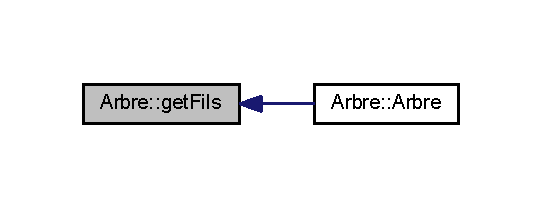
\includegraphics[width=260pt]{class_arbre_ace487e80301c07e6369108bf9a480513_icgraph}
\end{center}
\end{figure}
\mbox{\Hypertarget{class_arbre_a46ec1d0b89a9466c87a31e8e43133099}\label{class_arbre_a46ec1d0b89a9466c87a31e8e43133099}} 
\index{Arbre@{Arbre}!get\+Fils\+Indice@{get\+Fils\+Indice}}
\index{get\+Fils\+Indice@{get\+Fils\+Indice}!Arbre@{Arbre}}
\subsubsection{\texorpdfstring{get\+Fils\+Indice()}{getFilsIndice()}}
{\footnotesize\ttfamily \hyperlink{class_goban}{Goban} Arbre\+::get\+Fils\+Indice (\begin{DoxyParamCaption}\item[{const size\+\_\+t}]{indice }\end{DoxyParamCaption}) const}

\mbox{\Hypertarget{class_arbre_abb30fa37b209f6e148a5dc29e3a1c00d}\label{class_arbre_abb30fa37b209f6e148a5dc29e3a1c00d}} 
\index{Arbre@{Arbre}!get\+Gob@{get\+Gob}}
\index{get\+Gob@{get\+Gob}!Arbre@{Arbre}}
\subsubsection{\texorpdfstring{get\+Gob()}{getGob()}}
{\footnotesize\ttfamily \hyperlink{class_goban}{Goban} Arbre\+::get\+Gob (\begin{DoxyParamCaption}{ }\end{DoxyParamCaption}) const}

Here is the caller graph for this function\+:\nopagebreak
\begin{figure}[H]
\begin{center}
\leavevmode
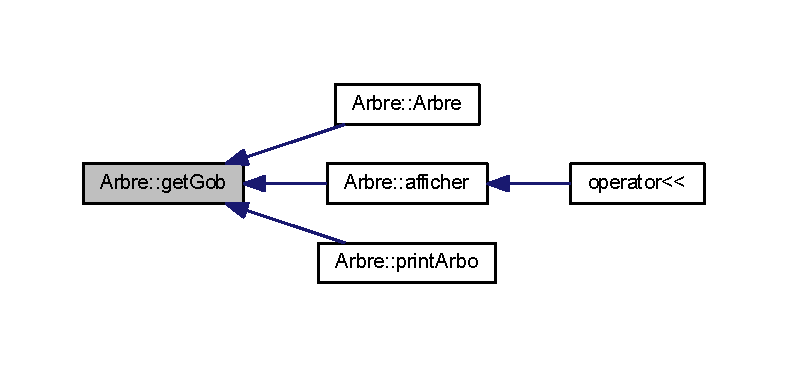
\includegraphics[width=350pt]{class_arbre_abb30fa37b209f6e148a5dc29e3a1c00d_icgraph}
\end{center}
\end{figure}
\mbox{\Hypertarget{class_arbre_afc71a182e86352b06193c2dc746fab79}\label{class_arbre_afc71a182e86352b06193c2dc746fab79}} 
\index{Arbre@{Arbre}!get\+Info@{get\+Info}}
\index{get\+Info@{get\+Info}!Arbre@{Arbre}}
\subsubsection{\texorpdfstring{get\+Info()}{getInfo()}}
{\footnotesize\ttfamily bool Arbre\+::get\+Info (\begin{DoxyParamCaption}{ }\end{DoxyParamCaption}) const}

\mbox{\Hypertarget{class_arbre_a0aef1f091d76bca13229a21fcd45a076}\label{class_arbre_a0aef1f091d76bca13229a21fcd45a076}} 
\index{Arbre@{Arbre}!get\+NbF@{get\+NbF}}
\index{get\+NbF@{get\+NbF}!Arbre@{Arbre}}
\subsubsection{\texorpdfstring{get\+Nb\+F()}{getNbF()}}
{\footnotesize\ttfamily size\+\_\+t Arbre\+::get\+NbF (\begin{DoxyParamCaption}{ }\end{DoxyParamCaption}) const}

Here is the caller graph for this function\+:\nopagebreak
\begin{figure}[H]
\begin{center}
\leavevmode
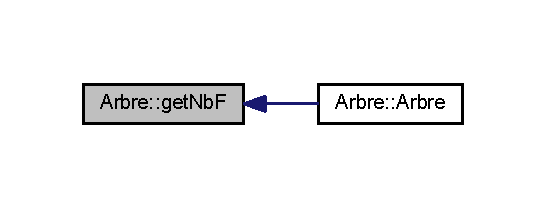
\includegraphics[width=262pt]{class_arbre_a0aef1f091d76bca13229a21fcd45a076_icgraph}
\end{center}
\end{figure}
\mbox{\Hypertarget{class_arbre_aeaa93d0b192e3cce04adb509b6b29c40}\label{class_arbre_aeaa93d0b192e3cce04adb509b6b29c40}} 
\index{Arbre@{Arbre}!get\+Value@{get\+Value}}
\index{get\+Value@{get\+Value}!Arbre@{Arbre}}
\subsubsection{\texorpdfstring{get\+Value()}{getValue()}}
{\footnotesize\ttfamily \hyperlink{class_etat_af3ddb2296ffc379b7f3ad2bf832f294e}{Etat\+::\+V\+AL} Arbre\+::get\+Value (\begin{DoxyParamCaption}{ }\end{DoxyParamCaption}) const}

Here is the caller graph for this function\+:\nopagebreak
\begin{figure}[H]
\begin{center}
\leavevmode
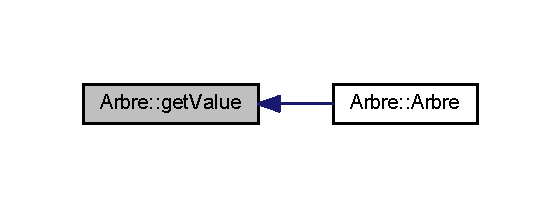
\includegraphics[width=269pt]{class_arbre_aeaa93d0b192e3cce04adb509b6b29c40_icgraph}
\end{center}
\end{figure}
\mbox{\Hypertarget{class_arbre_a2a919273c1041a7f024f717cdd638632}\label{class_arbre_a2a919273c1041a7f024f717cdd638632}} 
\index{Arbre@{Arbre}!operator=@{operator=}}
\index{operator=@{operator=}!Arbre@{Arbre}}
\subsubsection{\texorpdfstring{operator=()}{operator=()}}
{\footnotesize\ttfamily \hyperlink{class_arbre}{Arbre} Arbre\+::operator= (\begin{DoxyParamCaption}\item[{\hyperlink{class_arbre}{Arbre}}]{a }\end{DoxyParamCaption})}

\mbox{\Hypertarget{class_arbre_a8127785309368d2f2cd5a68f913e18cd}\label{class_arbre_a8127785309368d2f2cd5a68f913e18cd}} 
\index{Arbre@{Arbre}!operator\mbox{[}\mbox{]}@{operator[]}}
\index{operator\mbox{[}\mbox{]}@{operator[]}!Arbre@{Arbre}}
\subsubsection{\texorpdfstring{operator[]()}{operator[]()}}
{\footnotesize\ttfamily \hyperlink{class_goban}{Goban} Arbre\+::operator\mbox{[}$\,$\mbox{]} (\begin{DoxyParamCaption}\item[{unsigned short int}]{i }\end{DoxyParamCaption})}

\mbox{\Hypertarget{class_arbre_ac6329911b0037ca669e6ef2e12a178c9}\label{class_arbre_ac6329911b0037ca669e6ef2e12a178c9}} 
\index{Arbre@{Arbre}!print\+Arbo@{print\+Arbo}}
\index{print\+Arbo@{print\+Arbo}!Arbre@{Arbre}}
\subsubsection{\texorpdfstring{print\+Arbo()}{printArbo()}}
{\footnotesize\ttfamily void Arbre\+::print\+Arbo (\begin{DoxyParamCaption}\item[{const \hyperlink{class_arbre}{Arbre} \&}]{ }\end{DoxyParamCaption})}

Here is the call graph for this function\+:\nopagebreak
\begin{figure}[H]
\begin{center}
\leavevmode
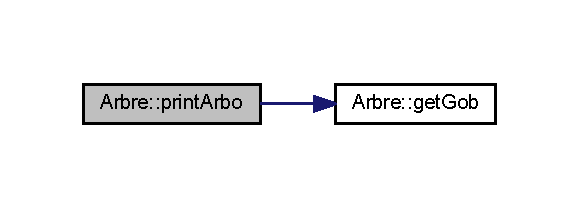
\includegraphics[width=278pt]{class_arbre_ac6329911b0037ca669e6ef2e12a178c9_cgraph}
\end{center}
\end{figure}
\mbox{\Hypertarget{class_arbre_ad7db2ec4bca90d9523c9dab19eadd628}\label{class_arbre_ad7db2ec4bca90d9523c9dab19eadd628}} 
\index{Arbre@{Arbre}!set\+Fils@{set\+Fils}}
\index{set\+Fils@{set\+Fils}!Arbre@{Arbre}}
\subsubsection{\texorpdfstring{set\+Fils()}{setFils()}}
{\footnotesize\ttfamily void Arbre\+::set\+Fils (\begin{DoxyParamCaption}\item[{\hyperlink{class_goban}{Goban}}]{f,  }\item[{const size\+\_\+t}]{i }\end{DoxyParamCaption})}

\mbox{\Hypertarget{class_arbre_a36267e74d40f509fd63b99fe6d8dae0b}\label{class_arbre_a36267e74d40f509fd63b99fe6d8dae0b}} 
\index{Arbre@{Arbre}!set\+Gob@{set\+Gob}}
\index{set\+Gob@{set\+Gob}!Arbre@{Arbre}}
\subsubsection{\texorpdfstring{set\+Gob()}{setGob()}}
{\footnotesize\ttfamily void Arbre\+::set\+Gob (\begin{DoxyParamCaption}\item[{\hyperlink{class_goban}{Goban}}]{\+\_\+gob }\end{DoxyParamCaption})}

\mbox{\Hypertarget{class_arbre_a051e5328c63ba7ab6f6359f9f2f77105}\label{class_arbre_a051e5328c63ba7ab6f6359f9f2f77105}} 
\index{Arbre@{Arbre}!set\+Info@{set\+Info}}
\index{set\+Info@{set\+Info}!Arbre@{Arbre}}
\subsubsection{\texorpdfstring{set\+Info()}{setInfo()}}
{\footnotesize\ttfamily void Arbre\+::set\+Info (\begin{DoxyParamCaption}\item[{bool}]{b }\end{DoxyParamCaption})}

\mbox{\Hypertarget{class_arbre_acabc45692262e5ca9c2f7b410ddcd373}\label{class_arbre_acabc45692262e5ca9c2f7b410ddcd373}} 
\index{Arbre@{Arbre}!set\+NbF@{set\+NbF}}
\index{set\+NbF@{set\+NbF}!Arbre@{Arbre}}
\subsubsection{\texorpdfstring{set\+Nb\+F()}{setNbF()}}
{\footnotesize\ttfamily void Arbre\+::set\+NbF (\begin{DoxyParamCaption}\item[{size\+\_\+t}]{\+\_\+nbF }\end{DoxyParamCaption})}

\mbox{\Hypertarget{class_arbre_a8108ffdff578e323dd9e50cc105a5c04}\label{class_arbre_a8108ffdff578e323dd9e50cc105a5c04}} 
\index{Arbre@{Arbre}!set\+Value@{set\+Value}}
\index{set\+Value@{set\+Value}!Arbre@{Arbre}}
\subsubsection{\texorpdfstring{set\+Value()}{setValue()}}
{\footnotesize\ttfamily void Arbre\+::set\+Value (\begin{DoxyParamCaption}\item[{\hyperlink{class_etat_af3ddb2296ffc379b7f3ad2bf832f294e}{Etat\+::\+V\+AL}}]{v }\end{DoxyParamCaption})}

\mbox{\Hypertarget{class_arbre_acd12cae4820bb7780a628716a0615d10}\label{class_arbre_acd12cae4820bb7780a628716a0615d10}} 
\index{Arbre@{Arbre}!Tsumego@{Tsumego}}
\index{Tsumego@{Tsumego}!Arbre@{Arbre}}
\subsubsection{\texorpdfstring{Tsumego()}{Tsumego()}}
{\footnotesize\ttfamily void Arbre\+::\+Tsumego (\begin{DoxyParamCaption}\item[{\hyperlink{class_etat}{Etat} \&}]{cible }\end{DoxyParamCaption})}

Here is the call graph for this function\+:\nopagebreak
\begin{figure}[H]
\begin{center}
\leavevmode
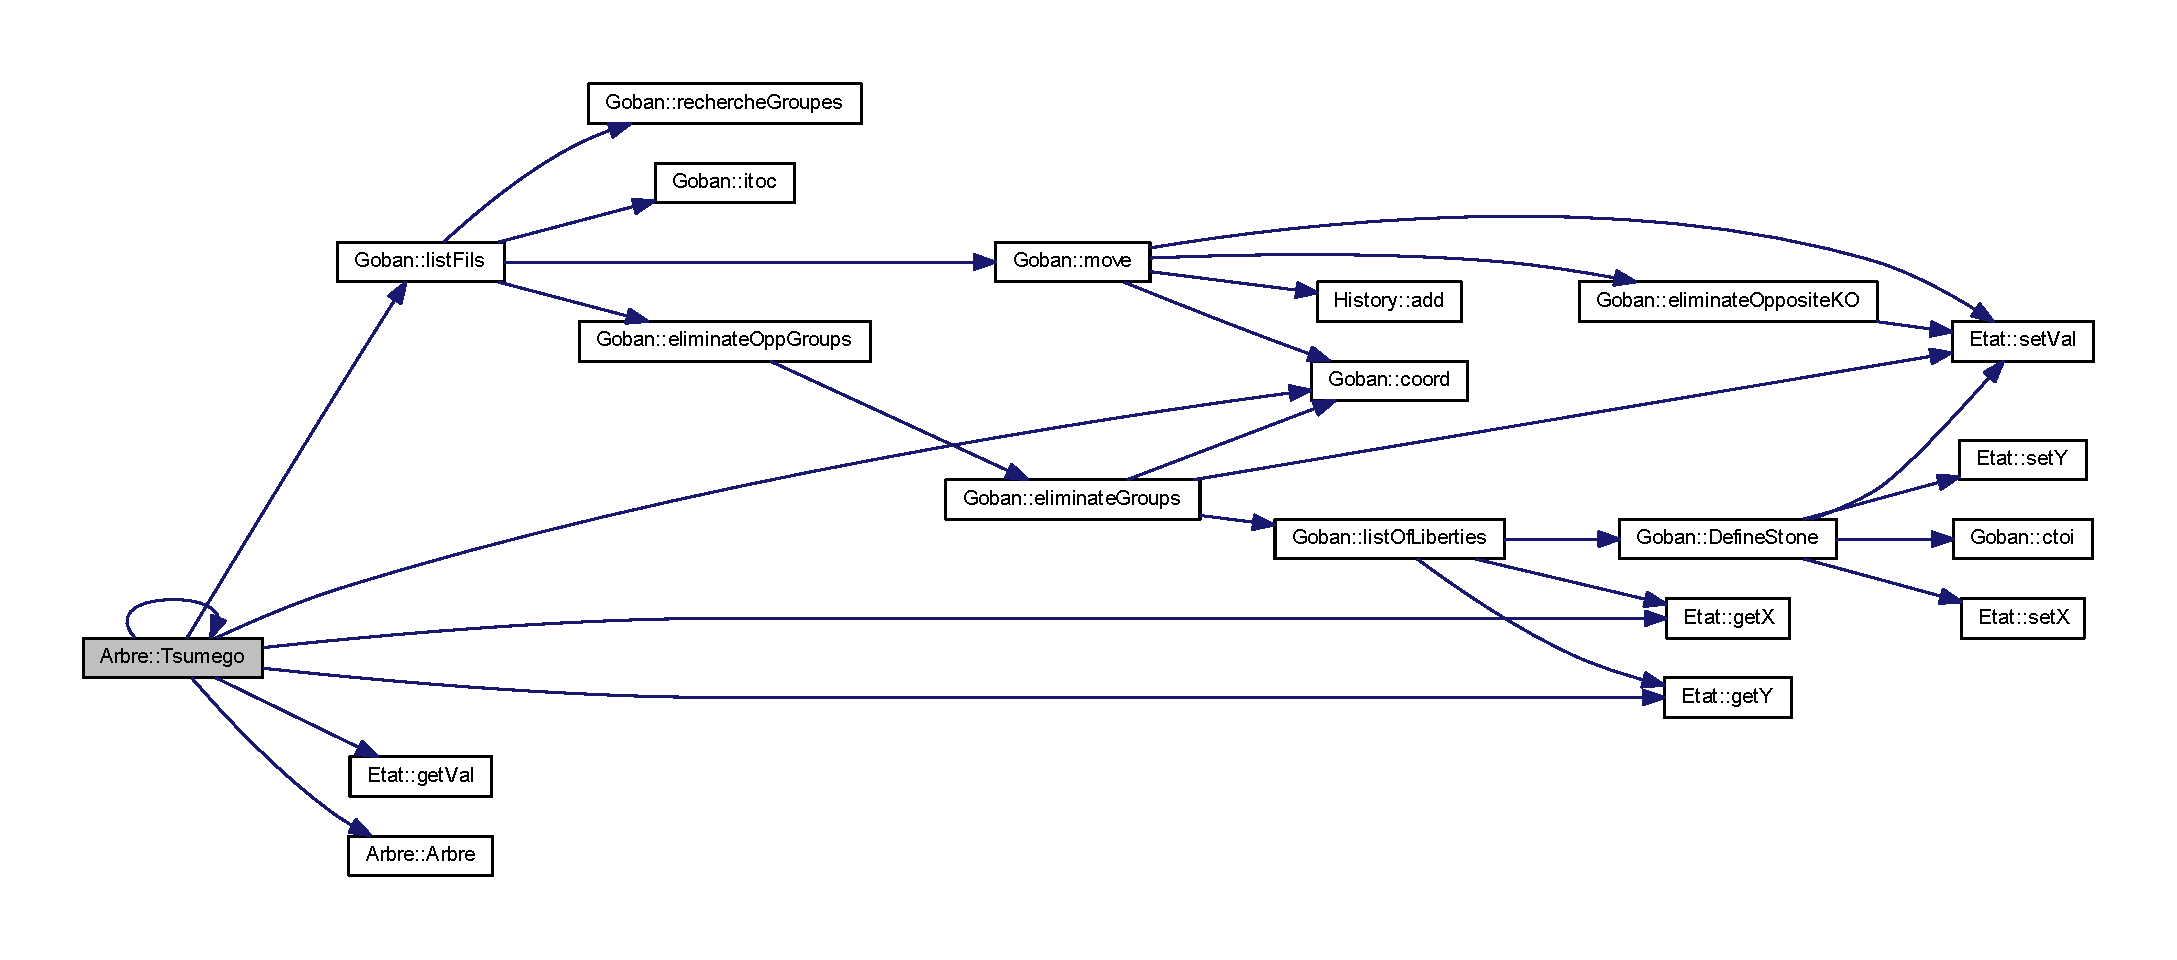
\includegraphics[width=350pt]{class_arbre_acd12cae4820bb7780a628716a0615d10_cgraph}
\end{center}
\end{figure}
Here is the caller graph for this function\+:\nopagebreak
\begin{figure}[H]
\begin{center}
\leavevmode
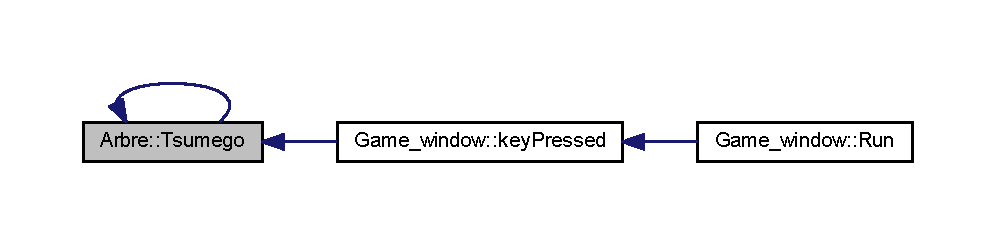
\includegraphics[width=350pt]{class_arbre_acd12cae4820bb7780a628716a0615d10_icgraph}
\end{center}
\end{figure}


The documentation for this class was generated from the following files\+:\begin{DoxyCompactItemize}
\item 
D\+:/\+Users/\+Victor/\+One\+Drive/\+Documents/\+Visual Studio 2017/\+Projects/\+Jeu\+\_\+de\+\_\+\+Go/\+Jeu\+\_\+de\+\_\+\+Go/\+Sources/\+Engine/\hyperlink{_arbre_8h}{Arbre.\+h}\item 
D\+:/\+Users/\+Victor/\+One\+Drive/\+Documents/\+Visual Studio 2017/\+Projects/\+Jeu\+\_\+de\+\_\+\+Go/\+Jeu\+\_\+de\+\_\+\+Go/\+Sources/\+Engine/\hyperlink{_arbre_8cpp}{Arbre.\+cpp}\end{DoxyCompactItemize}

\hypertarget{class_board}{}\section{Board Class Reference}
\label{class_board}\index{Board@{Board}}


{\ttfamily \#include $<$Board.\+h$>$}



Inheritance diagram for Board\+:
\nopagebreak
\begin{figure}[H]
\begin{center}
\leavevmode
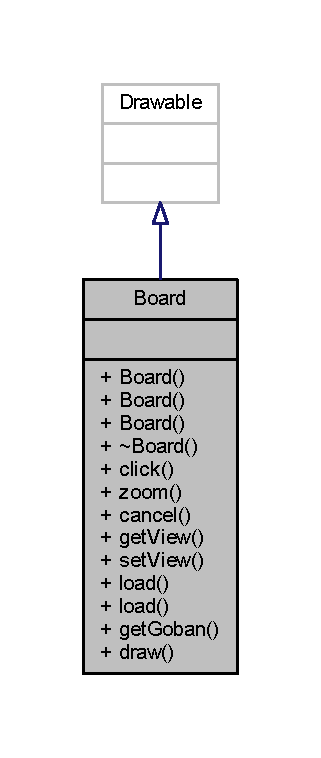
\includegraphics[width=185pt]{class_board__inherit__graph}
\end{center}
\end{figure}


Collaboration diagram for Board\+:
\nopagebreak
\begin{figure}[H]
\begin{center}
\leavevmode
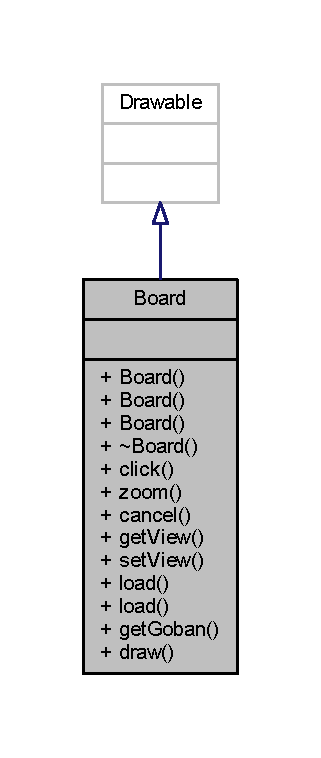
\includegraphics[width=185pt]{class_board__coll__graph}
\end{center}
\end{figure}
\subsection*{Public Member Functions}
\begin{DoxyCompactItemize}
\item 
\hyperlink{class_board_a9ee491d4fea680cf69b033374a9fdfcb}{Board} ()
\item 
{\footnotesize template$<$typename T $>$ }\\\hyperlink{class_board_a3ab3bc5a15b6f8fb4aa8473fed2afdcb}{Board} (const sf\+::\+Vector2$<$ T $>$ \&\+\_\+size)
\item 
{\footnotesize template$<$typename T $>$ }\\\hyperlink{class_board_abda1ce2449776e76715fc7b59c912935}{Board} (const T \&x, const T \&y)
\item 
\hyperlink{class_board_af73f45730119a1fd8f6670f53f959e68}{$\sim$\+Board} ()
\item 
bool \hyperlink{class_board_a5fda73da080403d8a71a8593d581c350}{click} (sf\+::\+Vector2i pos, const \hyperlink{class_square_a7feeec236c037a9849114226adaa4ecc}{Square\+::\+Value} \&value, const sf\+::\+Mouse\+::\+Button \&event)
\item 
void \hyperlink{class_board_a0b098808fd9214c752097a623a7c717e}{zoom} (const float delta, const sf\+::\+Vector2i \&pos)
\item 
void \hyperlink{class_board_ac7ec911a62371650afd340d1535a1742}{cancel} ()
\item 
sf\+::\+View \hyperlink{class_board_ad3c413e185668418d3a16c1fec68e70d}{get\+View} () const
\item 
void \hyperlink{class_board_afb8c7e3266134506f024b29e08fef695}{set\+View} (const sf\+::\+Float\+Rect \&zone)
\item 
void \hyperlink{class_board_a841a248dac4743611ba1825afd5d1297}{load} ()
\item 
void \hyperlink{class_board_a3cea4df16e41c21666cf51789b7e9e78}{load} (const \hyperlink{class_goban}{Goban} \&copy)
\item 
float \hyperlink{class_board_a061962e73609a58802ad83674ec9b413}{get\+Volume} () const
\item 
void \hyperlink{class_board_a4450fe85fda29736cd835fed63d40a41}{set\+Volume} (float vol)
\item 
void \hyperlink{class_board_a77d145afa8d71a85c4097aca08c30525}{turn\+Sounds\+Up} ()
\item 
void \hyperlink{class_board_a648552cb139f9c0cc61f6372251739b2}{turn\+Sounds\+Down} ()
\item 
\hyperlink{class_goban}{Goban} \hyperlink{class_board_a19af96f42f5c38336010da2983abbf5c}{get\+Goban} () const
\item 
virtual void \hyperlink{class_board_a8c86104f9ff30a54cbd7520e006cd609}{draw} (sf\+::\+Render\+Target \&target, sf\+::\+Render\+States states=sf\+::\+Render\+States\+::\+Default) const
\end{DoxyCompactItemize}


\subsection{Constructor \& Destructor Documentation}
\mbox{\Hypertarget{class_board_a9ee491d4fea680cf69b033374a9fdfcb}\label{class_board_a9ee491d4fea680cf69b033374a9fdfcb}} 
\index{Board@{Board}!Board@{Board}}
\index{Board@{Board}!Board@{Board}}
\subsubsection{\texorpdfstring{Board()}{Board()}\hspace{0.1cm}{\footnotesize\ttfamily [1/3]}}
{\footnotesize\ttfamily Board\+::\+Board (\begin{DoxyParamCaption}{ }\end{DoxyParamCaption})}

Here is the call graph for this function\+:
\nopagebreak
\begin{figure}[H]
\begin{center}
\leavevmode
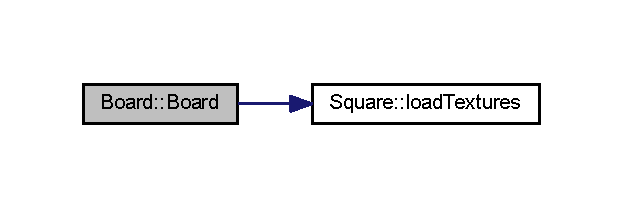
\includegraphics[width=299pt]{class_board_a9ee491d4fea680cf69b033374a9fdfcb_cgraph}
\end{center}
\end{figure}
\mbox{\Hypertarget{class_board_a3ab3bc5a15b6f8fb4aa8473fed2afdcb}\label{class_board_a3ab3bc5a15b6f8fb4aa8473fed2afdcb}} 
\index{Board@{Board}!Board@{Board}}
\index{Board@{Board}!Board@{Board}}
\subsubsection{\texorpdfstring{Board()}{Board()}\hspace{0.1cm}{\footnotesize\ttfamily [2/3]}}
{\footnotesize\ttfamily template$<$typename T $>$ \\
Board\+::\+Board (\begin{DoxyParamCaption}\item[{const sf\+::\+Vector2$<$ T $>$ \&}]{\+\_\+size }\end{DoxyParamCaption})}

Here is the call graph for this function\+:
\nopagebreak
\begin{figure}[H]
\begin{center}
\leavevmode
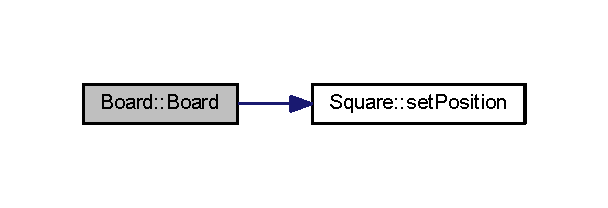
\includegraphics[width=292pt]{class_board_a3ab3bc5a15b6f8fb4aa8473fed2afdcb_cgraph}
\end{center}
\end{figure}
\mbox{\Hypertarget{class_board_abda1ce2449776e76715fc7b59c912935}\label{class_board_abda1ce2449776e76715fc7b59c912935}} 
\index{Board@{Board}!Board@{Board}}
\index{Board@{Board}!Board@{Board}}
\subsubsection{\texorpdfstring{Board()}{Board()}\hspace{0.1cm}{\footnotesize\ttfamily [3/3]}}
{\footnotesize\ttfamily template$<$typename T $>$ \\
Board\+::\+Board (\begin{DoxyParamCaption}\item[{const T \&}]{x,  }\item[{const T \&}]{y }\end{DoxyParamCaption})}

\mbox{\Hypertarget{class_board_af73f45730119a1fd8f6670f53f959e68}\label{class_board_af73f45730119a1fd8f6670f53f959e68}} 
\index{Board@{Board}!````~Board@{$\sim$\+Board}}
\index{````~Board@{$\sim$\+Board}!Board@{Board}}
\subsubsection{\texorpdfstring{$\sim$\+Board()}{~Board()}}
{\footnotesize\ttfamily Board\+::$\sim$\+Board (\begin{DoxyParamCaption}{ }\end{DoxyParamCaption})}



\subsection{Member Function Documentation}
\mbox{\Hypertarget{class_board_ac7ec911a62371650afd340d1535a1742}\label{class_board_ac7ec911a62371650afd340d1535a1742}} 
\index{Board@{Board}!cancel@{cancel}}
\index{cancel@{cancel}!Board@{Board}}
\subsubsection{\texorpdfstring{cancel()}{cancel()}}
{\footnotesize\ttfamily void Board\+::cancel (\begin{DoxyParamCaption}{ }\end{DoxyParamCaption})}

Here is the call graph for this function\+:
\nopagebreak
\begin{figure}[H]
\begin{center}
\leavevmode
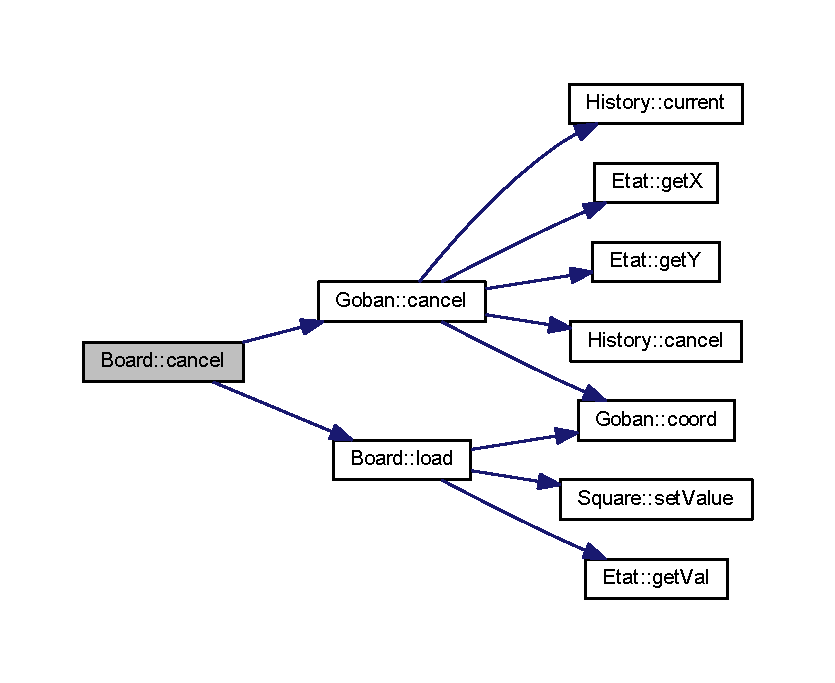
\includegraphics[width=350pt]{class_board_ac7ec911a62371650afd340d1535a1742_cgraph}
\end{center}
\end{figure}
Here is the caller graph for this function\+:
\nopagebreak
\begin{figure}[H]
\begin{center}
\leavevmode
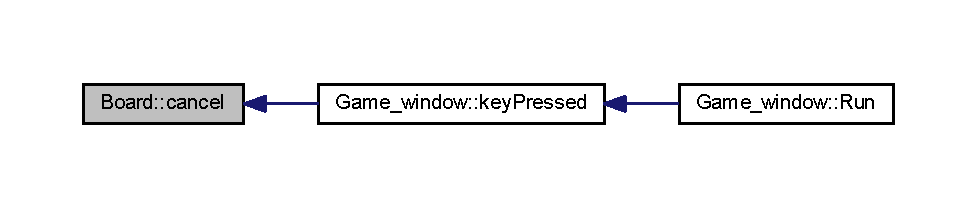
\includegraphics[width=350pt]{class_board_ac7ec911a62371650afd340d1535a1742_icgraph}
\end{center}
\end{figure}
\mbox{\Hypertarget{class_board_a5fda73da080403d8a71a8593d581c350}\label{class_board_a5fda73da080403d8a71a8593d581c350}} 
\index{Board@{Board}!click@{click}}
\index{click@{click}!Board@{Board}}
\subsubsection{\texorpdfstring{click()}{click()}}
{\footnotesize\ttfamily bool Board\+::click (\begin{DoxyParamCaption}\item[{sf\+::\+Vector2i}]{pos,  }\item[{const \hyperlink{class_square_a7feeec236c037a9849114226adaa4ecc}{Square\+::\+Value} \&}]{value,  }\item[{const sf\+::\+Mouse\+::\+Button \&}]{event }\end{DoxyParamCaption})}

Here is the call graph for this function\+:
\nopagebreak
\begin{figure}[H]
\begin{center}
\leavevmode
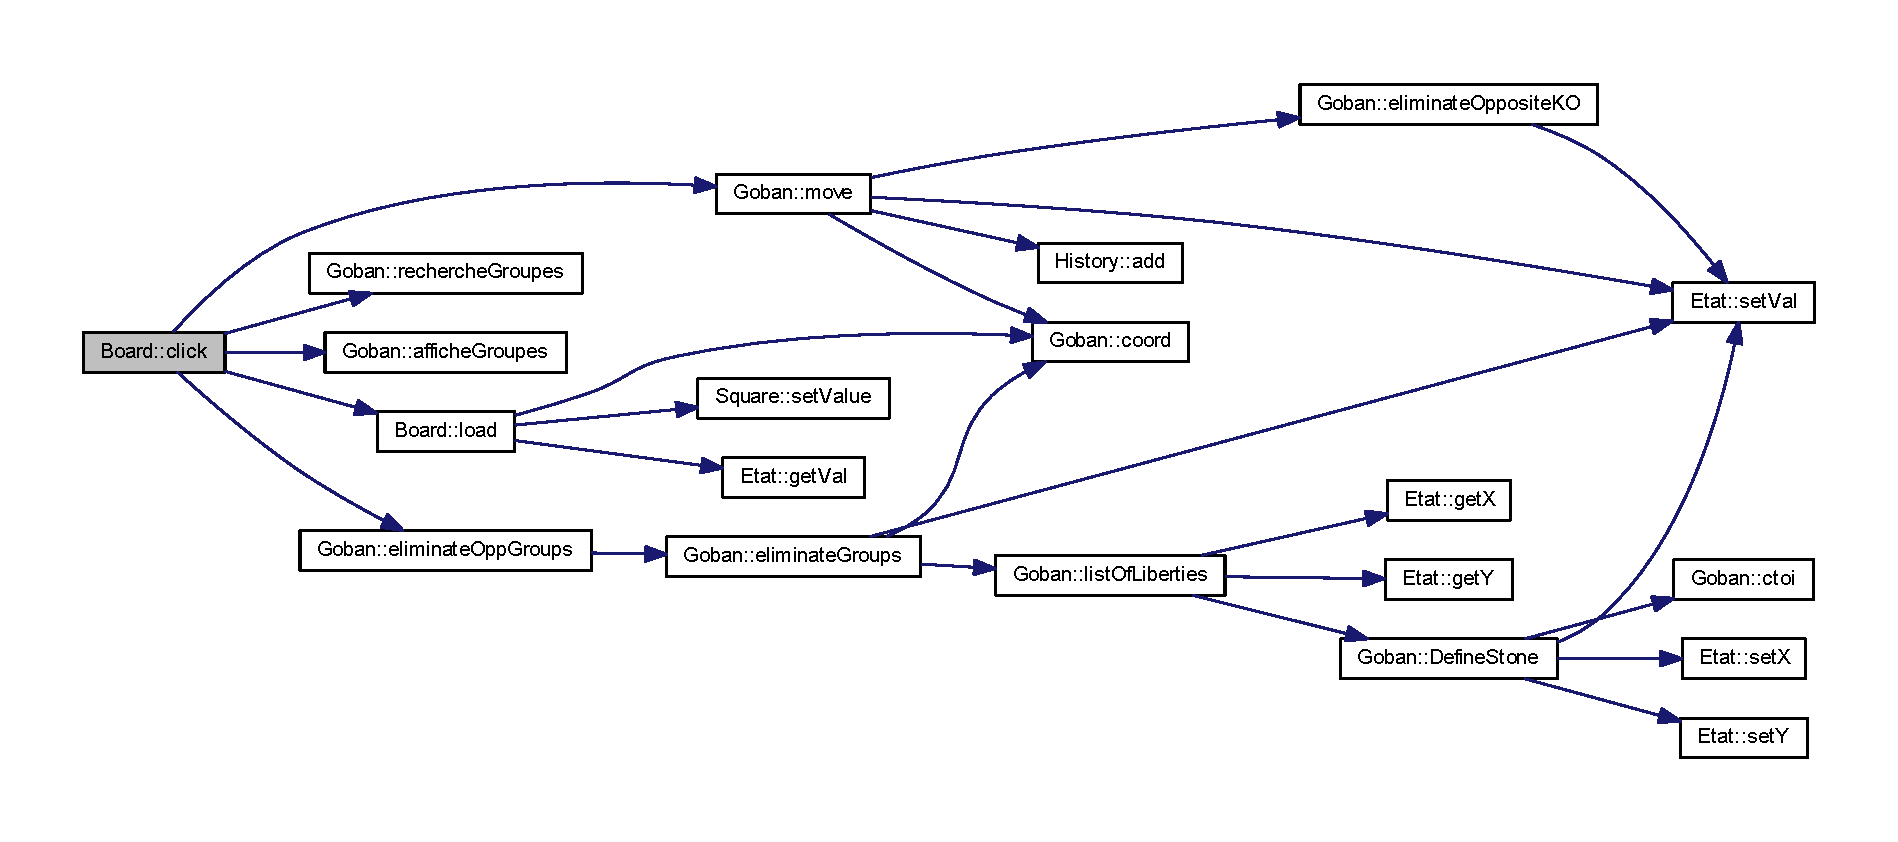
\includegraphics[width=350pt]{class_board_a5fda73da080403d8a71a8593d581c350_cgraph}
\end{center}
\end{figure}
Here is the caller graph for this function\+:
\nopagebreak
\begin{figure}[H]
\begin{center}
\leavevmode
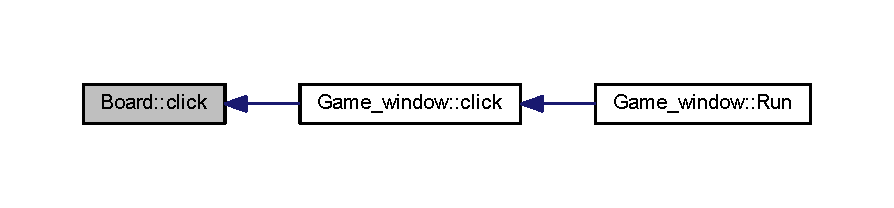
\includegraphics[width=350pt]{class_board_a5fda73da080403d8a71a8593d581c350_icgraph}
\end{center}
\end{figure}
\mbox{\Hypertarget{class_board_a8c86104f9ff30a54cbd7520e006cd609}\label{class_board_a8c86104f9ff30a54cbd7520e006cd609}} 
\index{Board@{Board}!draw@{draw}}
\index{draw@{draw}!Board@{Board}}
\subsubsection{\texorpdfstring{draw()}{draw()}}
{\footnotesize\ttfamily void Board\+::draw (\begin{DoxyParamCaption}\item[{sf\+::\+Render\+Target \&}]{target,  }\item[{sf\+::\+Render\+States}]{states = {\ttfamily sf\+:\+:RenderStates\+:\+:Default} }\end{DoxyParamCaption}) const\hspace{0.3cm}{\ttfamily [virtual]}}

Here is the call graph for this function\+:
\nopagebreak
\begin{figure}[H]
\begin{center}
\leavevmode
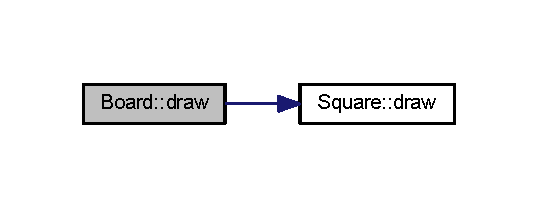
\includegraphics[width=258pt]{class_board_a8c86104f9ff30a54cbd7520e006cd609_cgraph}
\end{center}
\end{figure}
\mbox{\Hypertarget{class_board_a19af96f42f5c38336010da2983abbf5c}\label{class_board_a19af96f42f5c38336010da2983abbf5c}} 
\index{Board@{Board}!get\+Goban@{get\+Goban}}
\index{get\+Goban@{get\+Goban}!Board@{Board}}
\subsubsection{\texorpdfstring{get\+Goban()}{getGoban()}}
{\footnotesize\ttfamily \hyperlink{class_goban}{Goban} Board\+::get\+Goban (\begin{DoxyParamCaption}{ }\end{DoxyParamCaption}) const}

Here is the caller graph for this function\+:
\nopagebreak
\begin{figure}[H]
\begin{center}
\leavevmode
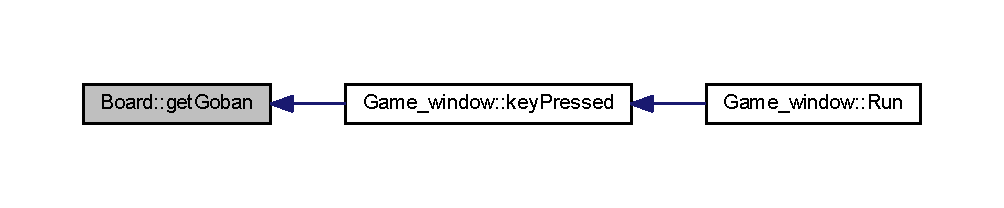
\includegraphics[width=350pt]{class_board_a19af96f42f5c38336010da2983abbf5c_icgraph}
\end{center}
\end{figure}
\mbox{\Hypertarget{class_board_ad3c413e185668418d3a16c1fec68e70d}\label{class_board_ad3c413e185668418d3a16c1fec68e70d}} 
\index{Board@{Board}!get\+View@{get\+View}}
\index{get\+View@{get\+View}!Board@{Board}}
\subsubsection{\texorpdfstring{get\+View()}{getView()}}
{\footnotesize\ttfamily sf\+::\+View Board\+::get\+View (\begin{DoxyParamCaption}{ }\end{DoxyParamCaption}) const}

Here is the caller graph for this function\+:
\nopagebreak
\begin{figure}[H]
\begin{center}
\leavevmode
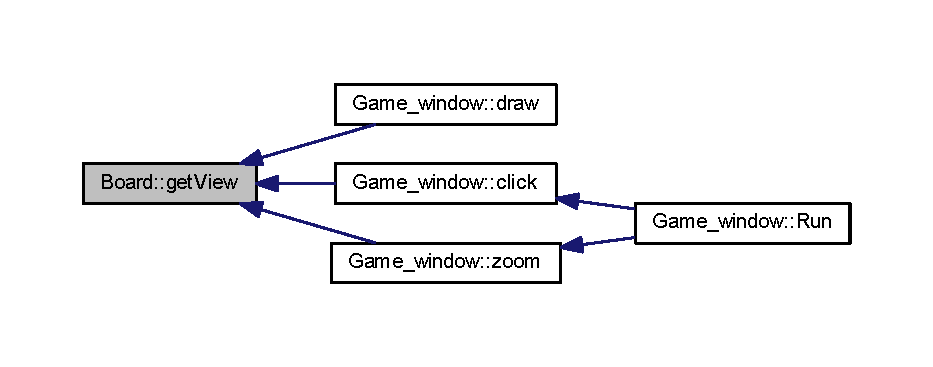
\includegraphics[width=350pt]{class_board_ad3c413e185668418d3a16c1fec68e70d_icgraph}
\end{center}
\end{figure}
\mbox{\Hypertarget{class_board_a061962e73609a58802ad83674ec9b413}\label{class_board_a061962e73609a58802ad83674ec9b413}} 
\index{Board@{Board}!get\+Volume@{get\+Volume}}
\index{get\+Volume@{get\+Volume}!Board@{Board}}
\subsubsection{\texorpdfstring{get\+Volume()}{getVolume()}}
{\footnotesize\ttfamily float Board\+::get\+Volume (\begin{DoxyParamCaption}{ }\end{DoxyParamCaption}) const}

Here is the caller graph for this function\+:
\nopagebreak
\begin{figure}[H]
\begin{center}
\leavevmode
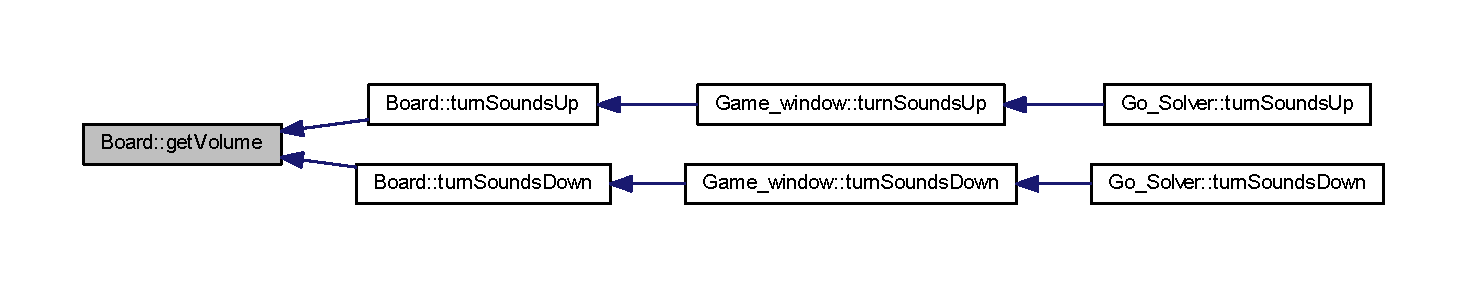
\includegraphics[width=350pt]{class_board_a061962e73609a58802ad83674ec9b413_icgraph}
\end{center}
\end{figure}
\mbox{\Hypertarget{class_board_a841a248dac4743611ba1825afd5d1297}\label{class_board_a841a248dac4743611ba1825afd5d1297}} 
\index{Board@{Board}!load@{load}}
\index{load@{load}!Board@{Board}}
\subsubsection{\texorpdfstring{load()}{load()}\hspace{0.1cm}{\footnotesize\ttfamily [1/2]}}
{\footnotesize\ttfamily void Board\+::load (\begin{DoxyParamCaption}{ }\end{DoxyParamCaption})}

Here is the call graph for this function\+:
\nopagebreak
\begin{figure}[H]
\begin{center}
\leavevmode
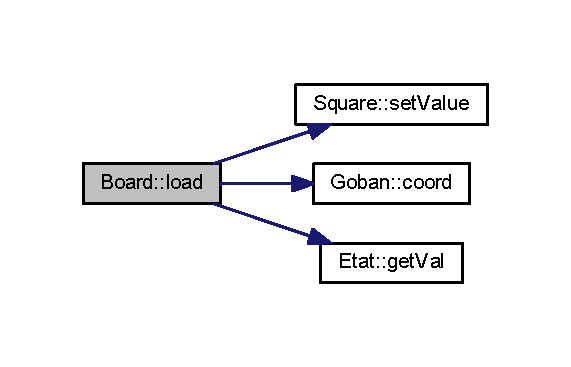
\includegraphics[width=274pt]{class_board_a841a248dac4743611ba1825afd5d1297_cgraph}
\end{center}
\end{figure}
Here is the caller graph for this function\+:
\nopagebreak
\begin{figure}[H]
\begin{center}
\leavevmode
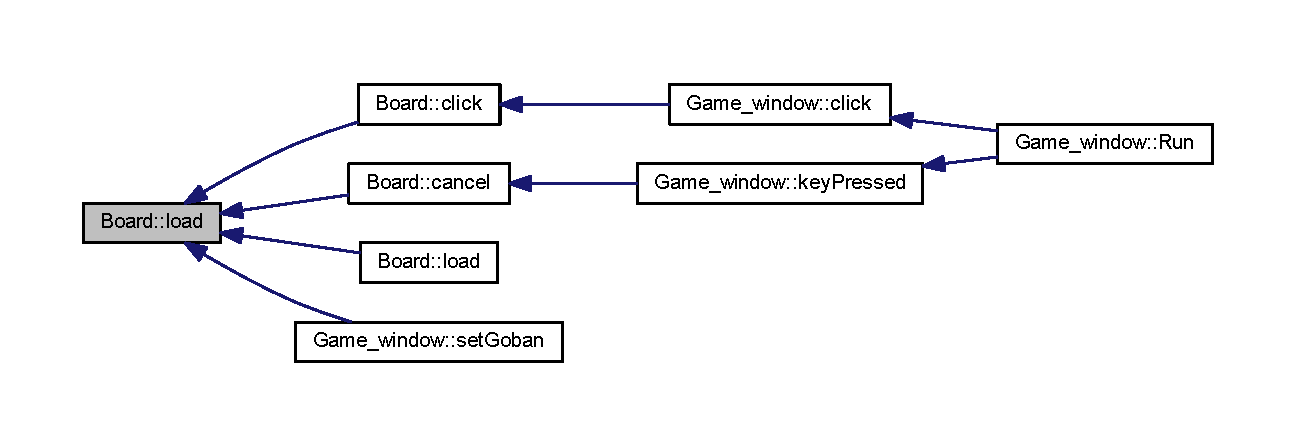
\includegraphics[width=350pt]{class_board_a841a248dac4743611ba1825afd5d1297_icgraph}
\end{center}
\end{figure}
\mbox{\Hypertarget{class_board_a3cea4df16e41c21666cf51789b7e9e78}\label{class_board_a3cea4df16e41c21666cf51789b7e9e78}} 
\index{Board@{Board}!load@{load}}
\index{load@{load}!Board@{Board}}
\subsubsection{\texorpdfstring{load()}{load()}\hspace{0.1cm}{\footnotesize\ttfamily [2/2]}}
{\footnotesize\ttfamily void Board\+::load (\begin{DoxyParamCaption}\item[{const \hyperlink{class_goban}{Goban} \&}]{copy }\end{DoxyParamCaption})}

Here is the call graph for this function\+:
\nopagebreak
\begin{figure}[H]
\begin{center}
\leavevmode
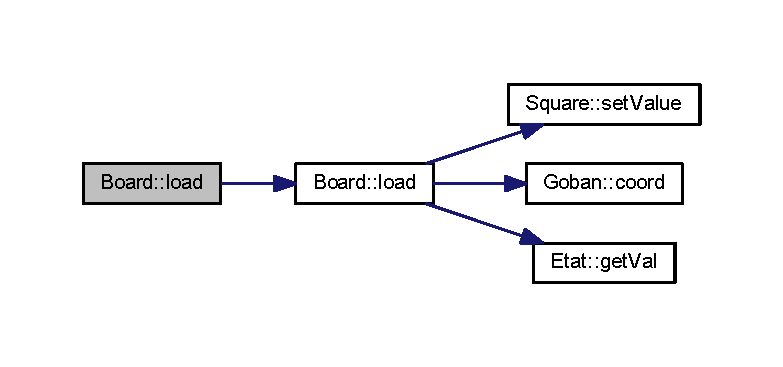
\includegraphics[width=350pt]{class_board_a3cea4df16e41c21666cf51789b7e9e78_cgraph}
\end{center}
\end{figure}
\mbox{\Hypertarget{class_board_afb8c7e3266134506f024b29e08fef695}\label{class_board_afb8c7e3266134506f024b29e08fef695}} 
\index{Board@{Board}!set\+View@{set\+View}}
\index{set\+View@{set\+View}!Board@{Board}}
\subsubsection{\texorpdfstring{set\+View()}{setView()}}
{\footnotesize\ttfamily void Board\+::set\+View (\begin{DoxyParamCaption}\item[{const sf\+::\+Float\+Rect \&}]{zone }\end{DoxyParamCaption})}

Here is the caller graph for this function\+:
\nopagebreak
\begin{figure}[H]
\begin{center}
\leavevmode
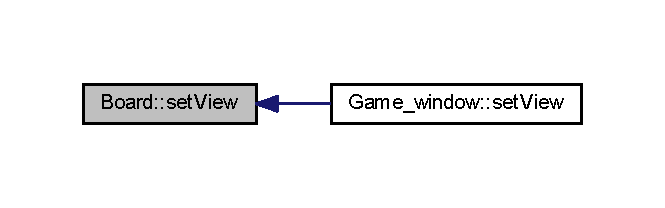
\includegraphics[width=319pt]{class_board_afb8c7e3266134506f024b29e08fef695_icgraph}
\end{center}
\end{figure}
\mbox{\Hypertarget{class_board_a4450fe85fda29736cd835fed63d40a41}\label{class_board_a4450fe85fda29736cd835fed63d40a41}} 
\index{Board@{Board}!set\+Volume@{set\+Volume}}
\index{set\+Volume@{set\+Volume}!Board@{Board}}
\subsubsection{\texorpdfstring{set\+Volume()}{setVolume()}}
{\footnotesize\ttfamily void Board\+::set\+Volume (\begin{DoxyParamCaption}\item[{float}]{vol }\end{DoxyParamCaption})}

Here is the caller graph for this function\+:
\nopagebreak
\begin{figure}[H]
\begin{center}
\leavevmode
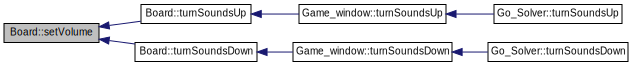
\includegraphics[width=350pt]{class_board_a4450fe85fda29736cd835fed63d40a41_icgraph}
\end{center}
\end{figure}
\mbox{\Hypertarget{class_board_a648552cb139f9c0cc61f6372251739b2}\label{class_board_a648552cb139f9c0cc61f6372251739b2}} 
\index{Board@{Board}!turn\+Sounds\+Down@{turn\+Sounds\+Down}}
\index{turn\+Sounds\+Down@{turn\+Sounds\+Down}!Board@{Board}}
\subsubsection{\texorpdfstring{turn\+Sounds\+Down()}{turnSoundsDown()}}
{\footnotesize\ttfamily void Board\+::turn\+Sounds\+Down (\begin{DoxyParamCaption}{ }\end{DoxyParamCaption})}

Here is the call graph for this function\+:
\nopagebreak
\begin{figure}[H]
\begin{center}
\leavevmode
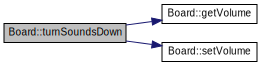
\includegraphics[width=333pt]{class_board_a648552cb139f9c0cc61f6372251739b2_cgraph}
\end{center}
\end{figure}
Here is the caller graph for this function\+:
\nopagebreak
\begin{figure}[H]
\begin{center}
\leavevmode
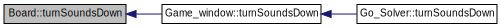
\includegraphics[width=350pt]{class_board_a648552cb139f9c0cc61f6372251739b2_icgraph}
\end{center}
\end{figure}
\mbox{\Hypertarget{class_board_a77d145afa8d71a85c4097aca08c30525}\label{class_board_a77d145afa8d71a85c4097aca08c30525}} 
\index{Board@{Board}!turn\+Sounds\+Up@{turn\+Sounds\+Up}}
\index{turn\+Sounds\+Up@{turn\+Sounds\+Up}!Board@{Board}}
\subsubsection{\texorpdfstring{turn\+Sounds\+Up()}{turnSoundsUp()}}
{\footnotesize\ttfamily void Board\+::turn\+Sounds\+Up (\begin{DoxyParamCaption}{ }\end{DoxyParamCaption})}

Here is the call graph for this function\+:
\nopagebreak
\begin{figure}[H]
\begin{center}
\leavevmode
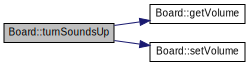
\includegraphics[width=321pt]{class_board_a77d145afa8d71a85c4097aca08c30525_cgraph}
\end{center}
\end{figure}
Here is the caller graph for this function\+:
\nopagebreak
\begin{figure}[H]
\begin{center}
\leavevmode
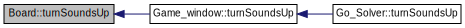
\includegraphics[width=350pt]{class_board_a77d145afa8d71a85c4097aca08c30525_icgraph}
\end{center}
\end{figure}
\mbox{\Hypertarget{class_board_a0b098808fd9214c752097a623a7c717e}\label{class_board_a0b098808fd9214c752097a623a7c717e}} 
\index{Board@{Board}!zoom@{zoom}}
\index{zoom@{zoom}!Board@{Board}}
\subsubsection{\texorpdfstring{zoom()}{zoom()}}
{\footnotesize\ttfamily void Board\+::zoom (\begin{DoxyParamCaption}\item[{const float}]{delta,  }\item[{const sf\+::\+Vector2i \&}]{pos }\end{DoxyParamCaption})}

Here is the caller graph for this function\+:
\nopagebreak
\begin{figure}[H]
\begin{center}
\leavevmode
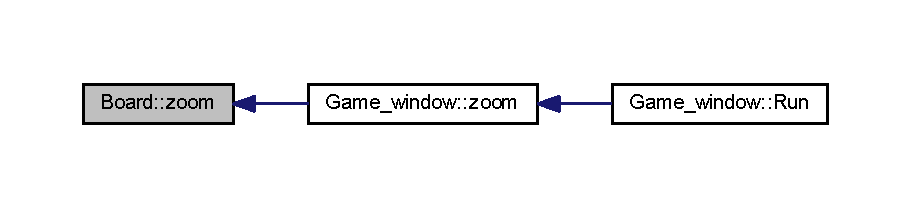
\includegraphics[width=350pt]{class_board_a0b098808fd9214c752097a623a7c717e_icgraph}
\end{center}
\end{figure}


The documentation for this class was generated from the following files\+:\begin{DoxyCompactItemize}
\item 
D\+:/\+Users/\+Victor/\+One\+Drive/\+Documents/\+Visual Studio 2017/\+Projects/\+Jeu\+\_\+de\+\_\+\+Go/\+Jeu\+\_\+de\+\_\+\+Go/\+Sources/\+Graphics/\+Game/\hyperlink{_board_8h}{Board.\+h}\item 
D\+:/\+Users/\+Victor/\+One\+Drive/\+Documents/\+Visual Studio 2017/\+Projects/\+Jeu\+\_\+de\+\_\+\+Go/\+Jeu\+\_\+de\+\_\+\+Go/\+Sources/\+Graphics/\+Game/\hyperlink{_board_8cpp}{Board.\+cpp}\end{DoxyCompactItemize}

\hypertarget{class_choice}{}\section{Choice Class Reference}
\label{class_choice}\index{Choice@{Choice}}


{\ttfamily \#include $<$Choice.\+h$>$}



Inheritance diagram for Choice\+:\nopagebreak
\begin{figure}[H]
\begin{center}
\leavevmode
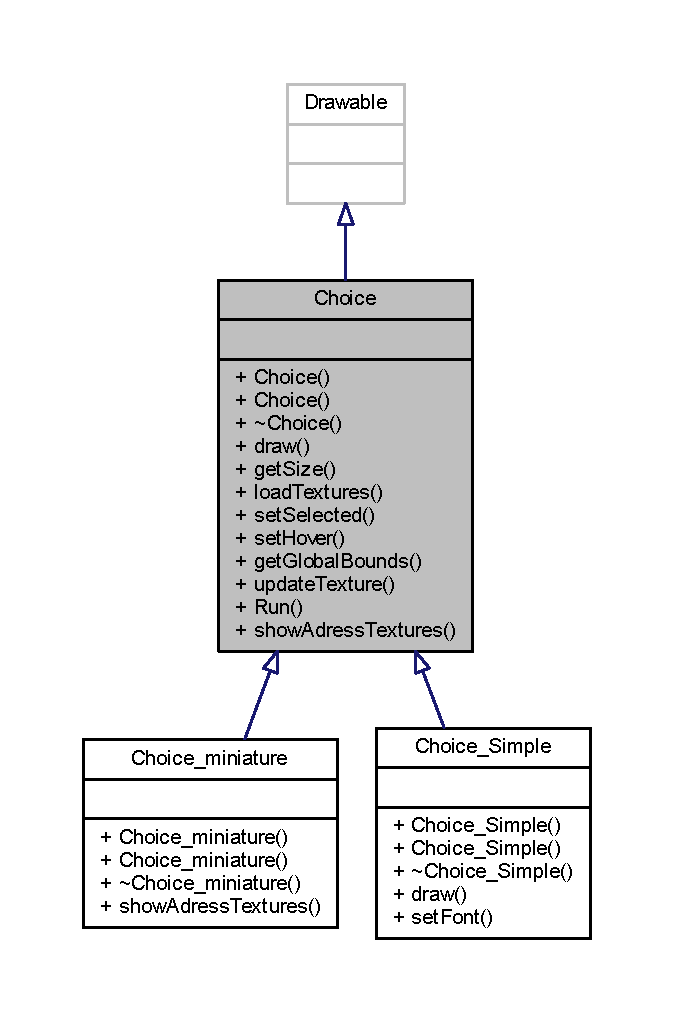
\includegraphics[width=324pt]{class_choice__inherit__graph}
\end{center}
\end{figure}


Collaboration diagram for Choice\+:\nopagebreak
\begin{figure}[H]
\begin{center}
\leavevmode
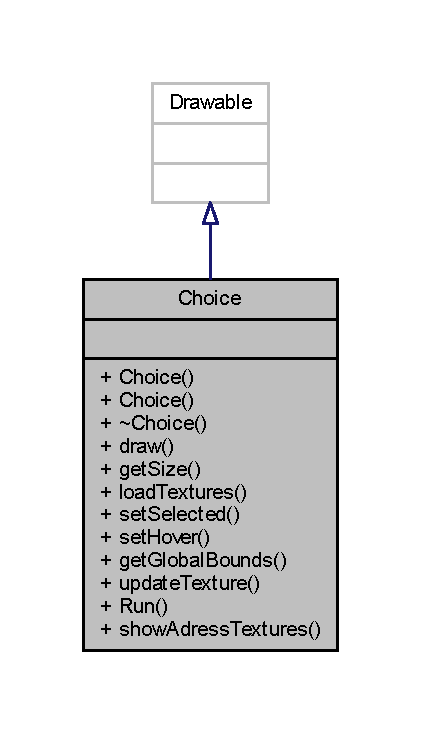
\includegraphics[width=202pt]{class_choice__coll__graph}
\end{center}
\end{figure}
\subsection*{Public Member Functions}
\begin{DoxyCompactItemize}
\item 
\hyperlink{class_choice_a0ce837a0b3bc6b119b06163482fba415}{Choice} (sf\+::\+Vector2f pos, std\+::function$<$ \hyperlink{_globals_8h_a3d5776bab98402b03be09156bacf4f68}{Screens}(const sf\+::\+Render\+Target \&, \hyperlink{class_game__window}{Game\+\_\+window} \&)$>$ \+\_\+\+Run, sf\+::\+Vector2f scale=sf\+::\+Vector2f(1, 1))
\item 
\hyperlink{class_choice_afc2877f32cc760f96f33d0a12a0c0911}{Choice} (float posX, float posY, std\+::function$<$ \hyperlink{_globals_8h_a3d5776bab98402b03be09156bacf4f68}{Screens}(const sf\+::\+Render\+Target \&, \hyperlink{class_game__window}{Game\+\_\+window} \&)$>$ \+\_\+\+Run, sf\+::\+Vector2f scale=sf\+::\+Vector2f(1, 1))
\item 
virtual \hyperlink{class_choice_ac60418c9d38713ccef3cb0dd1f14a083}{$\sim$\+Choice} ()
\item 
virtual void \hyperlink{class_choice_ad6a03ce8c892eacabef3691feba37b0f}{draw} (sf\+::\+Render\+Target \&target, sf\+::\+Render\+States states=sf\+::\+Render\+States\+::\+Default) const
\item 
sf\+::\+Vector2f \hyperlink{class_choice_ad013aa52558a29430889b9c6e9c0a1ab}{get\+Size} () const
\item 
virtual void \hyperlink{class_choice_a70d994feb4c3215eb477bae3df7c5052}{load\+Textures} (const sf\+::\+Texture $\ast$\+\_\+texture, const sf\+::\+Texture $\ast$selected, const sf\+::\+Texture $\ast$hover)
\item 
void \hyperlink{class_choice_aa4bbe520ca9f933327fc1f678d6626f8}{set\+Selected} (bool state=true)
\item 
void \hyperlink{class_choice_a377e5d456c5c7c7e8914af52cf184a3a}{set\+Hover} (bool state=true)
\item 
sf\+::\+Float\+Rect \hyperlink{class_choice_a8b901a892c521edcdb02c49c5bd057a8}{get\+Global\+Bounds} () const
\item 
void \hyperlink{class_choice_aa3113d895017610a03fff73795cf22fd}{update\+Texture} ()
\item 
\hyperlink{_globals_8h_a3d5776bab98402b03be09156bacf4f68}{Screens} \hyperlink{class_choice_aafd399c5b27102d38871a2a886eecd70}{Run} (const sf\+::\+Render\+Target \&window, \hyperlink{class_game__window}{Game\+\_\+window} \&game)
\item 
virtual void \hyperlink{class_choice_ad29163ceee43a59dba6ea46452ca46c0}{show\+Adress\+Textures} () const
\end{DoxyCompactItemize}


\subsection{Constructor \& Destructor Documentation}
\mbox{\Hypertarget{class_choice_a0ce837a0b3bc6b119b06163482fba415}\label{class_choice_a0ce837a0b3bc6b119b06163482fba415}} 
\index{Choice@{Choice}!Choice@{Choice}}
\index{Choice@{Choice}!Choice@{Choice}}
\subsubsection{\texorpdfstring{Choice()}{Choice()}\hspace{0.1cm}{\footnotesize\ttfamily [1/2]}}
{\footnotesize\ttfamily Choice\+::\+Choice (\begin{DoxyParamCaption}\item[{sf\+::\+Vector2f}]{pos,  }\item[{std\+::function$<$ \hyperlink{_globals_8h_a3d5776bab98402b03be09156bacf4f68}{Screens}(const sf\+::\+Render\+Target \&, \hyperlink{class_game__window}{Game\+\_\+window} \&)$>$}]{\+\_\+\+Run,  }\item[{sf\+::\+Vector2f}]{scale = {\ttfamily sf\+:\+:Vector2f(1,~1)} }\end{DoxyParamCaption})}

\mbox{\Hypertarget{class_choice_afc2877f32cc760f96f33d0a12a0c0911}\label{class_choice_afc2877f32cc760f96f33d0a12a0c0911}} 
\index{Choice@{Choice}!Choice@{Choice}}
\index{Choice@{Choice}!Choice@{Choice}}
\subsubsection{\texorpdfstring{Choice()}{Choice()}\hspace{0.1cm}{\footnotesize\ttfamily [2/2]}}
{\footnotesize\ttfamily Choice\+::\+Choice (\begin{DoxyParamCaption}\item[{float}]{posX,  }\item[{float}]{posY,  }\item[{std\+::function$<$ \hyperlink{_globals_8h_a3d5776bab98402b03be09156bacf4f68}{Screens}(const sf\+::\+Render\+Target \&, \hyperlink{class_game__window}{Game\+\_\+window} \&)$>$}]{\+\_\+\+Run,  }\item[{sf\+::\+Vector2f}]{scale = {\ttfamily sf\+:\+:Vector2f(1,~1)} }\end{DoxyParamCaption})}

\mbox{\Hypertarget{class_choice_ac60418c9d38713ccef3cb0dd1f14a083}\label{class_choice_ac60418c9d38713ccef3cb0dd1f14a083}} 
\index{Choice@{Choice}!````~Choice@{$\sim$\+Choice}}
\index{````~Choice@{$\sim$\+Choice}!Choice@{Choice}}
\subsubsection{\texorpdfstring{$\sim$\+Choice()}{~Choice()}}
{\footnotesize\ttfamily Choice\+::$\sim$\+Choice (\begin{DoxyParamCaption}{ }\end{DoxyParamCaption})\hspace{0.3cm}{\ttfamily [virtual]}}



\subsection{Member Function Documentation}
\mbox{\Hypertarget{class_choice_ad6a03ce8c892eacabef3691feba37b0f}\label{class_choice_ad6a03ce8c892eacabef3691feba37b0f}} 
\index{Choice@{Choice}!draw@{draw}}
\index{draw@{draw}!Choice@{Choice}}
\subsubsection{\texorpdfstring{draw()}{draw()}}
{\footnotesize\ttfamily void Choice\+::draw (\begin{DoxyParamCaption}\item[{sf\+::\+Render\+Target \&}]{target,  }\item[{sf\+::\+Render\+States}]{states = {\ttfamily sf\+:\+:RenderStates\+:\+:Default} }\end{DoxyParamCaption}) const\hspace{0.3cm}{\ttfamily [virtual]}}



Reimplemented in \hyperlink{class_choice___simple_ae8f4cedc34a10d3c35efce8cec1bec54}{Choice\+\_\+\+Simple}.

Here is the caller graph for this function\+:\nopagebreak
\begin{figure}[H]
\begin{center}
\leavevmode
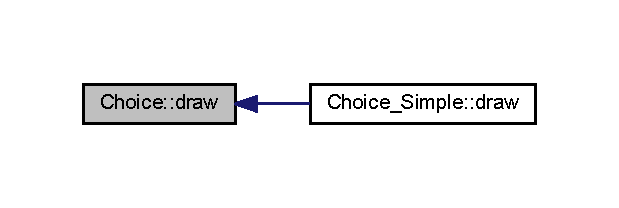
\includegraphics[width=297pt]{class_choice_ad6a03ce8c892eacabef3691feba37b0f_icgraph}
\end{center}
\end{figure}
\mbox{\Hypertarget{class_choice_a8b901a892c521edcdb02c49c5bd057a8}\label{class_choice_a8b901a892c521edcdb02c49c5bd057a8}} 
\index{Choice@{Choice}!get\+Global\+Bounds@{get\+Global\+Bounds}}
\index{get\+Global\+Bounds@{get\+Global\+Bounds}!Choice@{Choice}}
\subsubsection{\texorpdfstring{get\+Global\+Bounds()}{getGlobalBounds()}}
{\footnotesize\ttfamily sf\+::\+Float\+Rect Choice\+::get\+Global\+Bounds (\begin{DoxyParamCaption}{ }\end{DoxyParamCaption}) const}

\mbox{\Hypertarget{class_choice_ad013aa52558a29430889b9c6e9c0a1ab}\label{class_choice_ad013aa52558a29430889b9c6e9c0a1ab}} 
\index{Choice@{Choice}!get\+Size@{get\+Size}}
\index{get\+Size@{get\+Size}!Choice@{Choice}}
\subsubsection{\texorpdfstring{get\+Size()}{getSize()}}
{\footnotesize\ttfamily sf\+::\+Vector2f Choice\+::get\+Size (\begin{DoxyParamCaption}{ }\end{DoxyParamCaption}) const}

\mbox{\Hypertarget{class_choice_a70d994feb4c3215eb477bae3df7c5052}\label{class_choice_a70d994feb4c3215eb477bae3df7c5052}} 
\index{Choice@{Choice}!load\+Textures@{load\+Textures}}
\index{load\+Textures@{load\+Textures}!Choice@{Choice}}
\subsubsection{\texorpdfstring{load\+Textures()}{loadTextures()}}
{\footnotesize\ttfamily void Choice\+::load\+Textures (\begin{DoxyParamCaption}\item[{const sf\+::\+Texture $\ast$}]{\+\_\+texture,  }\item[{const sf\+::\+Texture $\ast$}]{selected,  }\item[{const sf\+::\+Texture $\ast$}]{hover }\end{DoxyParamCaption})\hspace{0.3cm}{\ttfamily [virtual]}}

Here is the call graph for this function\+:\nopagebreak
\begin{figure}[H]
\begin{center}
\leavevmode
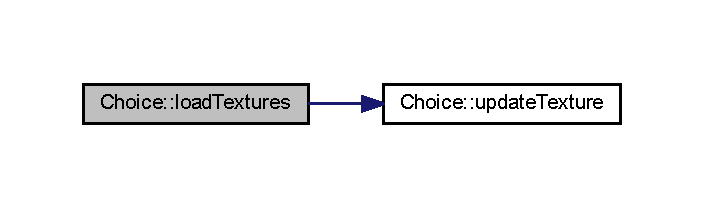
\includegraphics[width=338pt]{class_choice_a70d994feb4c3215eb477bae3df7c5052_cgraph}
\end{center}
\end{figure}
Here is the caller graph for this function\+:\nopagebreak
\begin{figure}[H]
\begin{center}
\leavevmode
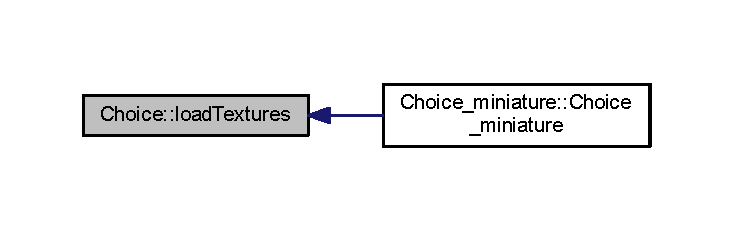
\includegraphics[width=350pt]{class_choice_a70d994feb4c3215eb477bae3df7c5052_icgraph}
\end{center}
\end{figure}
\mbox{\Hypertarget{class_choice_aafd399c5b27102d38871a2a886eecd70}\label{class_choice_aafd399c5b27102d38871a2a886eecd70}} 
\index{Choice@{Choice}!Run@{Run}}
\index{Run@{Run}!Choice@{Choice}}
\subsubsection{\texorpdfstring{Run()}{Run()}}
{\footnotesize\ttfamily \hyperlink{_globals_8h_a3d5776bab98402b03be09156bacf4f68}{Screens} Choice\+::\+Run (\begin{DoxyParamCaption}\item[{const sf\+::\+Render\+Target \&}]{window,  }\item[{\hyperlink{class_game__window}{Game\+\_\+window} \&}]{game }\end{DoxyParamCaption})}

Here is the caller graph for this function\+:\nopagebreak
\begin{figure}[H]
\begin{center}
\leavevmode
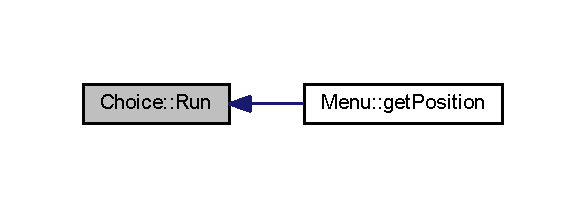
\includegraphics[width=281pt]{class_choice_aafd399c5b27102d38871a2a886eecd70_icgraph}
\end{center}
\end{figure}
\mbox{\Hypertarget{class_choice_a377e5d456c5c7c7e8914af52cf184a3a}\label{class_choice_a377e5d456c5c7c7e8914af52cf184a3a}} 
\index{Choice@{Choice}!set\+Hover@{set\+Hover}}
\index{set\+Hover@{set\+Hover}!Choice@{Choice}}
\subsubsection{\texorpdfstring{set\+Hover()}{setHover()}}
{\footnotesize\ttfamily void Choice\+::set\+Hover (\begin{DoxyParamCaption}\item[{bool}]{state = {\ttfamily true} }\end{DoxyParamCaption})}

Here is the call graph for this function\+:\nopagebreak
\begin{figure}[H]
\begin{center}
\leavevmode
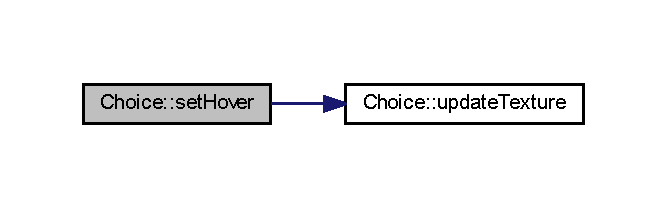
\includegraphics[width=320pt]{class_choice_a377e5d456c5c7c7e8914af52cf184a3a_cgraph}
\end{center}
\end{figure}
\mbox{\Hypertarget{class_choice_aa4bbe520ca9f933327fc1f678d6626f8}\label{class_choice_aa4bbe520ca9f933327fc1f678d6626f8}} 
\index{Choice@{Choice}!set\+Selected@{set\+Selected}}
\index{set\+Selected@{set\+Selected}!Choice@{Choice}}
\subsubsection{\texorpdfstring{set\+Selected()}{setSelected()}}
{\footnotesize\ttfamily void Choice\+::set\+Selected (\begin{DoxyParamCaption}\item[{bool}]{state = {\ttfamily true} }\end{DoxyParamCaption})}

Here is the call graph for this function\+:\nopagebreak
\begin{figure}[H]
\begin{center}
\leavevmode
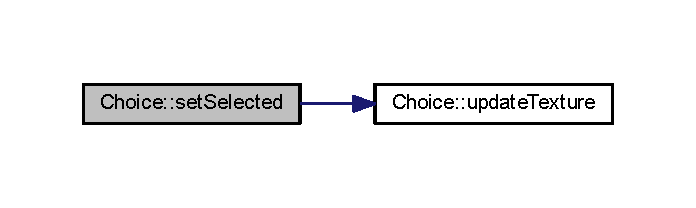
\includegraphics[width=334pt]{class_choice_aa4bbe520ca9f933327fc1f678d6626f8_cgraph}
\end{center}
\end{figure}
Here is the caller graph for this function\+:\nopagebreak
\begin{figure}[H]
\begin{center}
\leavevmode
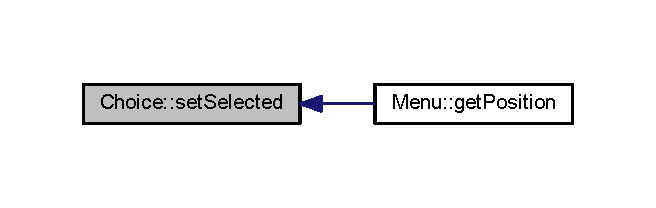
\includegraphics[width=315pt]{class_choice_aa4bbe520ca9f933327fc1f678d6626f8_icgraph}
\end{center}
\end{figure}
\mbox{\Hypertarget{class_choice_ad29163ceee43a59dba6ea46452ca46c0}\label{class_choice_ad29163ceee43a59dba6ea46452ca46c0}} 
\index{Choice@{Choice}!show\+Adress\+Textures@{show\+Adress\+Textures}}
\index{show\+Adress\+Textures@{show\+Adress\+Textures}!Choice@{Choice}}
\subsubsection{\texorpdfstring{show\+Adress\+Textures()}{showAdressTextures()}}
{\footnotesize\ttfamily void Choice\+::show\+Adress\+Textures (\begin{DoxyParamCaption}{ }\end{DoxyParamCaption}) const\hspace{0.3cm}{\ttfamily [virtual]}}



Reimplemented in \hyperlink{class_choice__miniature_a6f413024d98b0c334c5a3e6ec87eba9b}{Choice\+\_\+miniature}.

Here is the caller graph for this function\+:\nopagebreak
\begin{figure}[H]
\begin{center}
\leavevmode
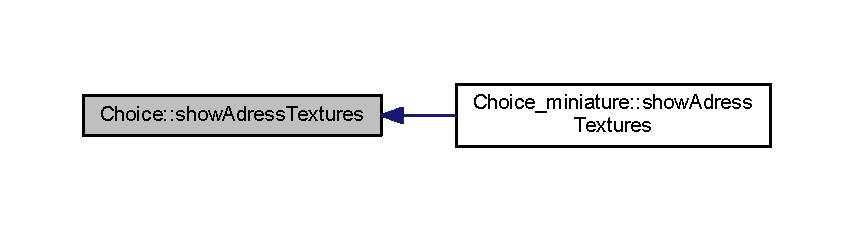
\includegraphics[width=350pt]{class_choice_ad29163ceee43a59dba6ea46452ca46c0_icgraph}
\end{center}
\end{figure}
\mbox{\Hypertarget{class_choice_aa3113d895017610a03fff73795cf22fd}\label{class_choice_aa3113d895017610a03fff73795cf22fd}} 
\index{Choice@{Choice}!update\+Texture@{update\+Texture}}
\index{update\+Texture@{update\+Texture}!Choice@{Choice}}
\subsubsection{\texorpdfstring{update\+Texture()}{updateTexture()}}
{\footnotesize\ttfamily void Choice\+::update\+Texture (\begin{DoxyParamCaption}{ }\end{DoxyParamCaption})}

Here is the caller graph for this function\+:\nopagebreak
\begin{figure}[H]
\begin{center}
\leavevmode
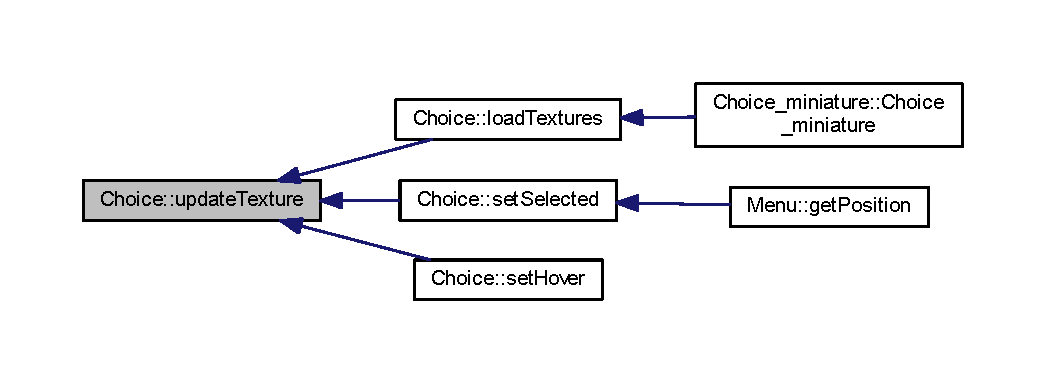
\includegraphics[width=350pt]{class_choice_aa3113d895017610a03fff73795cf22fd_icgraph}
\end{center}
\end{figure}


The documentation for this class was generated from the following files\+:\begin{DoxyCompactItemize}
\item 
D\+:/\+Users/\+Victor/\+One\+Drive/\+Documents/\+Visual Studio 2017/\+Projects/\+Jeu\+\_\+de\+\_\+\+Go/\+Jeu\+\_\+de\+\_\+\+Go/\+Sources/\+Graphics/\hyperlink{_choice_8h}{Choice.\+h}\item 
D\+:/\+Users/\+Victor/\+One\+Drive/\+Documents/\+Visual Studio 2017/\+Projects/\+Jeu\+\_\+de\+\_\+\+Go/\+Jeu\+\_\+de\+\_\+\+Go/\+Sources/\+Graphics/\hyperlink{_choice_8cpp}{Choice.\+cpp}\end{DoxyCompactItemize}

\hypertarget{class_choice__miniature}{}\section{Choice\+\_\+miniature Class Reference}
\label{class_choice__miniature}\index{Choice\+\_\+miniature@{Choice\+\_\+miniature}}


{\ttfamily \#include $<$Choice\+\_\+miniature.\+h$>$}



Inheritance diagram for Choice\+\_\+miniature\+:
\nopagebreak
\begin{figure}[H]
\begin{center}
\leavevmode
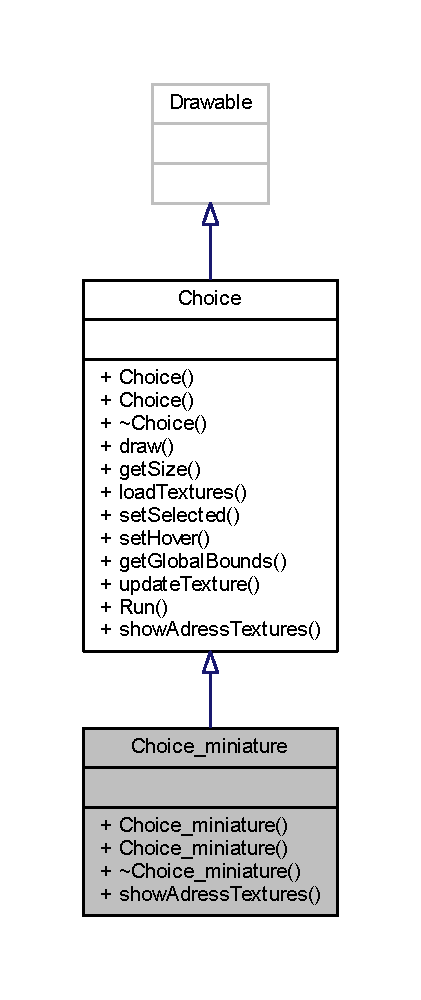
\includegraphics[width=202pt]{class_choice__miniature__inherit__graph}
\end{center}
\end{figure}


Collaboration diagram for Choice\+\_\+miniature\+:
\nopagebreak
\begin{figure}[H]
\begin{center}
\leavevmode
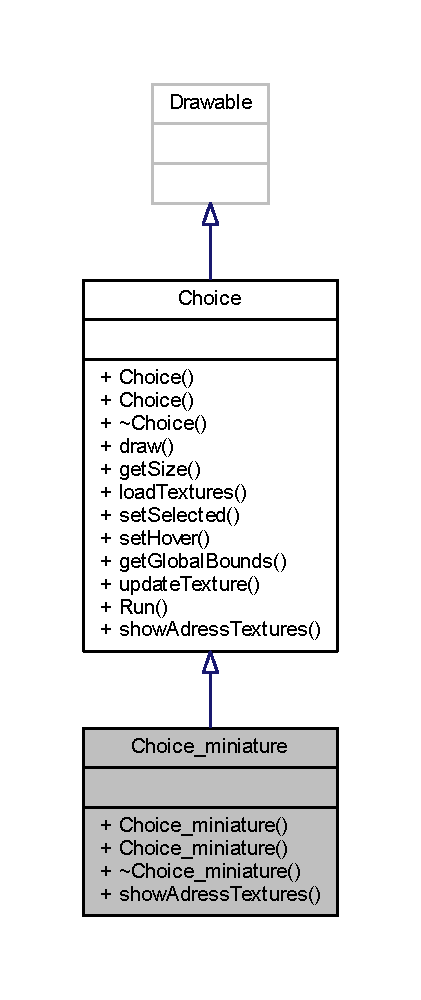
\includegraphics[width=202pt]{class_choice__miniature__coll__graph}
\end{center}
\end{figure}
\subsection*{Public Member Functions}
\begin{DoxyCompactItemize}
\item 
\hyperlink{class_choice__miniature_a156cdcafd4f44bdcf262669612fa8b82}{Choice\+\_\+miniature} (const char $\ast$\+\_\+texture, sf\+::\+Vector2f pos, std\+::function$<$ \hyperlink{_globals_8h_a3d5776bab98402b03be09156bacf4f68}{Screens}(sf\+::\+Render\+Target \&, \hyperlink{class_go___solver}{Go\+\_\+\+Solver} \&)$>$ \+\_\+\+Run, sf\+::\+Vector2f scale=sf\+::\+Vector2f(1, 1))
\item 
\hyperlink{class_choice__miniature_a0eee4352ef523c2d640a847ad016295d}{Choice\+\_\+miniature} (const char $\ast$\+\_\+texture, float posX, float posY, std\+::function$<$ \hyperlink{_globals_8h_a3d5776bab98402b03be09156bacf4f68}{Screens}(sf\+::\+Render\+Target \&, \hyperlink{class_go___solver}{Go\+\_\+\+Solver} \&)$>$ \+\_\+\+Run, sf\+::\+Vector2f scale=sf\+::\+Vector2f(1, 1))
\item 
virtual \hyperlink{class_choice__miniature_aa04b8d4c3ad3e99efad7ffe433d96fbe}{$\sim$\+Choice\+\_\+miniature} ()
\item 
virtual void \hyperlink{class_choice__miniature_a6f413024d98b0c334c5a3e6ec87eba9b}{show\+Adress\+Textures} () const
\end{DoxyCompactItemize}


\subsection{Constructor \& Destructor Documentation}
\mbox{\Hypertarget{class_choice__miniature_a156cdcafd4f44bdcf262669612fa8b82}\label{class_choice__miniature_a156cdcafd4f44bdcf262669612fa8b82}} 
\index{Choice\+\_\+miniature@{Choice\+\_\+miniature}!Choice\+\_\+miniature@{Choice\+\_\+miniature}}
\index{Choice\+\_\+miniature@{Choice\+\_\+miniature}!Choice\+\_\+miniature@{Choice\+\_\+miniature}}
\subsubsection{\texorpdfstring{Choice\+\_\+miniature()}{Choice\_miniature()}\hspace{0.1cm}{\footnotesize\ttfamily [1/2]}}
{\footnotesize\ttfamily Choice\+\_\+miniature\+::\+Choice\+\_\+miniature (\begin{DoxyParamCaption}\item[{const char $\ast$}]{\+\_\+texture,  }\item[{sf\+::\+Vector2f}]{pos,  }\item[{std\+::function$<$ \hyperlink{_globals_8h_a3d5776bab98402b03be09156bacf4f68}{Screens}(sf\+::\+Render\+Target \&, \hyperlink{class_go___solver}{Go\+\_\+\+Solver} \&)$>$}]{\+\_\+\+Run,  }\item[{sf\+::\+Vector2f}]{scale = {\ttfamily sf\+:\+:Vector2f(1,~1)} }\end{DoxyParamCaption})}

Here is the call graph for this function\+:
\nopagebreak
\begin{figure}[H]
\begin{center}
\leavevmode
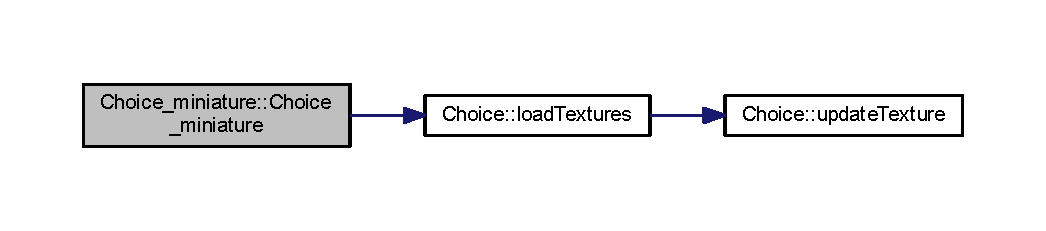
\includegraphics[width=350pt]{class_choice__miniature_a156cdcafd4f44bdcf262669612fa8b82_cgraph}
\end{center}
\end{figure}
\mbox{\Hypertarget{class_choice__miniature_a0eee4352ef523c2d640a847ad016295d}\label{class_choice__miniature_a0eee4352ef523c2d640a847ad016295d}} 
\index{Choice\+\_\+miniature@{Choice\+\_\+miniature}!Choice\+\_\+miniature@{Choice\+\_\+miniature}}
\index{Choice\+\_\+miniature@{Choice\+\_\+miniature}!Choice\+\_\+miniature@{Choice\+\_\+miniature}}
\subsubsection{\texorpdfstring{Choice\+\_\+miniature()}{Choice\_miniature()}\hspace{0.1cm}{\footnotesize\ttfamily [2/2]}}
{\footnotesize\ttfamily Choice\+\_\+miniature\+::\+Choice\+\_\+miniature (\begin{DoxyParamCaption}\item[{const char $\ast$}]{\+\_\+texture,  }\item[{float}]{posX,  }\item[{float}]{posY,  }\item[{std\+::function$<$ \hyperlink{_globals_8h_a3d5776bab98402b03be09156bacf4f68}{Screens}(sf\+::\+Render\+Target \&, \hyperlink{class_go___solver}{Go\+\_\+\+Solver} \&)$>$}]{\+\_\+\+Run,  }\item[{sf\+::\+Vector2f}]{scale = {\ttfamily sf\+:\+:Vector2f(1,~1)} }\end{DoxyParamCaption})}

\mbox{\Hypertarget{class_choice__miniature_aa04b8d4c3ad3e99efad7ffe433d96fbe}\label{class_choice__miniature_aa04b8d4c3ad3e99efad7ffe433d96fbe}} 
\index{Choice\+\_\+miniature@{Choice\+\_\+miniature}!````~Choice\+\_\+miniature@{$\sim$\+Choice\+\_\+miniature}}
\index{````~Choice\+\_\+miniature@{$\sim$\+Choice\+\_\+miniature}!Choice\+\_\+miniature@{Choice\+\_\+miniature}}
\subsubsection{\texorpdfstring{$\sim$\+Choice\+\_\+miniature()}{~Choice\_miniature()}}
{\footnotesize\ttfamily Choice\+\_\+miniature\+::$\sim$\+Choice\+\_\+miniature (\begin{DoxyParamCaption}{ }\end{DoxyParamCaption})\hspace{0.3cm}{\ttfamily [virtual]}}



\subsection{Member Function Documentation}
\mbox{\Hypertarget{class_choice__miniature_a6f413024d98b0c334c5a3e6ec87eba9b}\label{class_choice__miniature_a6f413024d98b0c334c5a3e6ec87eba9b}} 
\index{Choice\+\_\+miniature@{Choice\+\_\+miniature}!show\+Adress\+Textures@{show\+Adress\+Textures}}
\index{show\+Adress\+Textures@{show\+Adress\+Textures}!Choice\+\_\+miniature@{Choice\+\_\+miniature}}
\subsubsection{\texorpdfstring{show\+Adress\+Textures()}{showAdressTextures()}}
{\footnotesize\ttfamily void Choice\+\_\+miniature\+::show\+Adress\+Textures (\begin{DoxyParamCaption}{ }\end{DoxyParamCaption}) const\hspace{0.3cm}{\ttfamily [virtual]}}



Reimplemented from \hyperlink{class_choice_ad29163ceee43a59dba6ea46452ca46c0}{Choice}.

Here is the call graph for this function\+:
\nopagebreak
\begin{figure}[H]
\begin{center}
\leavevmode
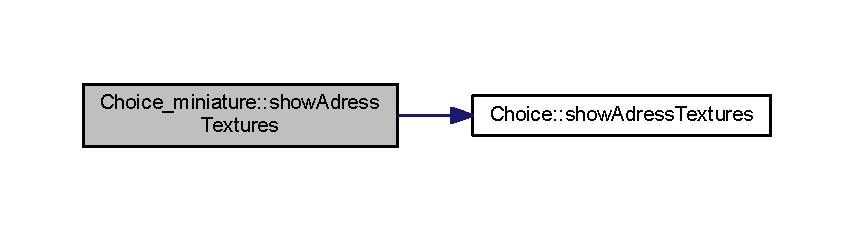
\includegraphics[width=350pt]{class_choice__miniature_a6f413024d98b0c334c5a3e6ec87eba9b_cgraph}
\end{center}
\end{figure}


The documentation for this class was generated from the following files\+:\begin{DoxyCompactItemize}
\item 
D\+:/\+Users/\+Victor/\+One\+Drive/\+Documents/\+Visual Studio 2017/\+Projects/\+Jeu\+\_\+de\+\_\+\+Go/\+Jeu\+\_\+de\+\_\+\+Go/\+Sources/\+Graphics/\hyperlink{_choice__miniature_8h}{Choice\+\_\+miniature.\+h}\item 
D\+:/\+Users/\+Victor/\+One\+Drive/\+Documents/\+Visual Studio 2017/\+Projects/\+Jeu\+\_\+de\+\_\+\+Go/\+Jeu\+\_\+de\+\_\+\+Go/\+Sources/\+Graphics/\hyperlink{_choice__miniature_8cpp}{Choice\+\_\+miniature.\+cpp}\end{DoxyCompactItemize}

\hypertarget{class_choice___simple}{}\section{Choice\+\_\+\+Simple Class Reference}
\label{class_choice___simple}\index{Choice\+\_\+\+Simple@{Choice\+\_\+\+Simple}}


{\ttfamily \#include $<$Choice\+\_\+\+Simple.\+h$>$}



Inheritance diagram for Choice\+\_\+\+Simple\+:
\nopagebreak
\begin{figure}[H]
\begin{center}
\leavevmode
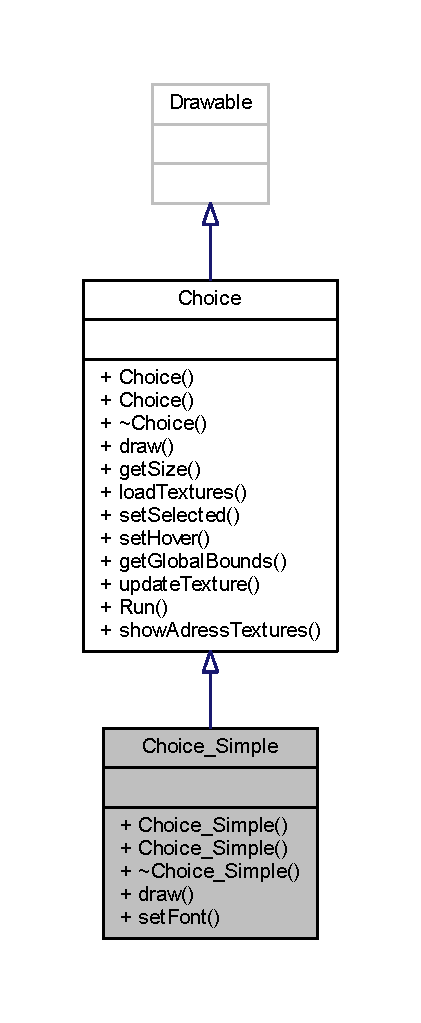
\includegraphics[width=202pt]{class_choice___simple__inherit__graph}
\end{center}
\end{figure}


Collaboration diagram for Choice\+\_\+\+Simple\+:
\nopagebreak
\begin{figure}[H]
\begin{center}
\leavevmode
\includegraphics[width=202pt]{class_choice___simple__coll__graph}
\end{center}
\end{figure}
\subsection*{Public Member Functions}
\begin{DoxyCompactItemize}
\item 
\hyperlink{class_choice___simple_aba8dc060adb5b2f393bbfb3d09127761}{Choice\+\_\+\+Simple} (const char $\ast$name, const sf\+::\+Text \&text\+\_\+style, sf\+::\+Vector2f pos, std\+::function$<$ \hyperlink{_globals_8h_a3d5776bab98402b03be09156bacf4f68}{Screens}(sf\+::\+Render\+Target \&, \hyperlink{class_go___solver}{Go\+\_\+\+Solver} \&)$>$ \+\_\+\+Run, sf\+::\+Vector2f scale=sf\+::\+Vector2f(1, 1))
\item 
\hyperlink{class_choice___simple_a00412cfa29b144f0aca041b93fab4b26}{Choice\+\_\+\+Simple} (const char $\ast$name, const sf\+::\+Text \&text\+\_\+style, float posX, float posY, std\+::function$<$ \hyperlink{_globals_8h_a3d5776bab98402b03be09156bacf4f68}{Screens}(sf\+::\+Render\+Target \&, \hyperlink{class_go___solver}{Go\+\_\+\+Solver} \&)$>$ \+\_\+\+Run, sf\+::\+Vector2f scale=sf\+::\+Vector2f(1, 1))
\item 
virtual \hyperlink{class_choice___simple_a6d5b3fe8aa2969f8eaffa4e5fd3b47d9}{$\sim$\+Choice\+\_\+\+Simple} ()
\item 
virtual void \hyperlink{class_choice___simple_ae8f4cedc34a10d3c35efce8cec1bec54}{draw} (sf\+::\+Render\+Target \&target, sf\+::\+Render\+States states=sf\+::\+Render\+States\+::\+Default) const
\item 
void \hyperlink{class_choice___simple_a035e32f90e4561b666b6571bce06e207}{set\+Font} (const sf\+::\+Font \&\+\_\+font)
\end{DoxyCompactItemize}


\subsection{Constructor \& Destructor Documentation}
\mbox{\Hypertarget{class_choice___simple_aba8dc060adb5b2f393bbfb3d09127761}\label{class_choice___simple_aba8dc060adb5b2f393bbfb3d09127761}} 
\index{Choice\+\_\+\+Simple@{Choice\+\_\+\+Simple}!Choice\+\_\+\+Simple@{Choice\+\_\+\+Simple}}
\index{Choice\+\_\+\+Simple@{Choice\+\_\+\+Simple}!Choice\+\_\+\+Simple@{Choice\+\_\+\+Simple}}
\subsubsection{\texorpdfstring{Choice\+\_\+\+Simple()}{Choice\_Simple()}\hspace{0.1cm}{\footnotesize\ttfamily [1/2]}}
{\footnotesize\ttfamily Choice\+\_\+\+Simple\+::\+Choice\+\_\+\+Simple (\begin{DoxyParamCaption}\item[{const char $\ast$}]{name,  }\item[{const sf\+::\+Text \&}]{text\+\_\+style,  }\item[{sf\+::\+Vector2f}]{pos,  }\item[{std\+::function$<$ \hyperlink{_globals_8h_a3d5776bab98402b03be09156bacf4f68}{Screens}(sf\+::\+Render\+Target \&, \hyperlink{class_go___solver}{Go\+\_\+\+Solver} \&)$>$}]{\+\_\+\+Run,  }\item[{sf\+::\+Vector2f}]{scale = {\ttfamily sf\+:\+:Vector2f(1,~1)} }\end{DoxyParamCaption})}

\mbox{\Hypertarget{class_choice___simple_a00412cfa29b144f0aca041b93fab4b26}\label{class_choice___simple_a00412cfa29b144f0aca041b93fab4b26}} 
\index{Choice\+\_\+\+Simple@{Choice\+\_\+\+Simple}!Choice\+\_\+\+Simple@{Choice\+\_\+\+Simple}}
\index{Choice\+\_\+\+Simple@{Choice\+\_\+\+Simple}!Choice\+\_\+\+Simple@{Choice\+\_\+\+Simple}}
\subsubsection{\texorpdfstring{Choice\+\_\+\+Simple()}{Choice\_Simple()}\hspace{0.1cm}{\footnotesize\ttfamily [2/2]}}
{\footnotesize\ttfamily Choice\+\_\+\+Simple\+::\+Choice\+\_\+\+Simple (\begin{DoxyParamCaption}\item[{const char $\ast$}]{name,  }\item[{const sf\+::\+Text \&}]{text\+\_\+style,  }\item[{float}]{posX,  }\item[{float}]{posY,  }\item[{std\+::function$<$ \hyperlink{_globals_8h_a3d5776bab98402b03be09156bacf4f68}{Screens}(sf\+::\+Render\+Target \&, \hyperlink{class_go___solver}{Go\+\_\+\+Solver} \&)$>$}]{\+\_\+\+Run,  }\item[{sf\+::\+Vector2f}]{scale = {\ttfamily sf\+:\+:Vector2f(1,~1)} }\end{DoxyParamCaption})}

\mbox{\Hypertarget{class_choice___simple_a6d5b3fe8aa2969f8eaffa4e5fd3b47d9}\label{class_choice___simple_a6d5b3fe8aa2969f8eaffa4e5fd3b47d9}} 
\index{Choice\+\_\+\+Simple@{Choice\+\_\+\+Simple}!````~Choice\+\_\+\+Simple@{$\sim$\+Choice\+\_\+\+Simple}}
\index{````~Choice\+\_\+\+Simple@{$\sim$\+Choice\+\_\+\+Simple}!Choice\+\_\+\+Simple@{Choice\+\_\+\+Simple}}
\subsubsection{\texorpdfstring{$\sim$\+Choice\+\_\+\+Simple()}{~Choice\_Simple()}}
{\footnotesize\ttfamily Choice\+\_\+\+Simple\+::$\sim$\+Choice\+\_\+\+Simple (\begin{DoxyParamCaption}{ }\end{DoxyParamCaption})\hspace{0.3cm}{\ttfamily [virtual]}}



\subsection{Member Function Documentation}
\mbox{\Hypertarget{class_choice___simple_ae8f4cedc34a10d3c35efce8cec1bec54}\label{class_choice___simple_ae8f4cedc34a10d3c35efce8cec1bec54}} 
\index{Choice\+\_\+\+Simple@{Choice\+\_\+\+Simple}!draw@{draw}}
\index{draw@{draw}!Choice\+\_\+\+Simple@{Choice\+\_\+\+Simple}}
\subsubsection{\texorpdfstring{draw()}{draw()}}
{\footnotesize\ttfamily void Choice\+\_\+\+Simple\+::draw (\begin{DoxyParamCaption}\item[{sf\+::\+Render\+Target \&}]{target,  }\item[{sf\+::\+Render\+States}]{states = {\ttfamily sf\+:\+:RenderStates\+:\+:Default} }\end{DoxyParamCaption}) const\hspace{0.3cm}{\ttfamily [virtual]}}



Reimplemented from \hyperlink{class_choice_ad6a03ce8c892eacabef3691feba37b0f}{Choice}.

Here is the call graph for this function\+:
\nopagebreak
\begin{figure}[H]
\begin{center}
\leavevmode
\includegraphics[width=297pt]{class_choice___simple_ae8f4cedc34a10d3c35efce8cec1bec54_cgraph}
\end{center}
\end{figure}
\mbox{\Hypertarget{class_choice___simple_a035e32f90e4561b666b6571bce06e207}\label{class_choice___simple_a035e32f90e4561b666b6571bce06e207}} 
\index{Choice\+\_\+\+Simple@{Choice\+\_\+\+Simple}!set\+Font@{set\+Font}}
\index{set\+Font@{set\+Font}!Choice\+\_\+\+Simple@{Choice\+\_\+\+Simple}}
\subsubsection{\texorpdfstring{set\+Font()}{setFont()}}
{\footnotesize\ttfamily void Choice\+\_\+\+Simple\+::set\+Font (\begin{DoxyParamCaption}\item[{const sf\+::\+Font \&}]{\+\_\+font }\end{DoxyParamCaption})}

Here is the caller graph for this function\+:
\nopagebreak
\begin{figure}[H]
\begin{center}
\leavevmode
\includegraphics[width=350pt]{class_choice___simple_a035e32f90e4561b666b6571bce06e207_icgraph}
\end{center}
\end{figure}


The documentation for this class was generated from the following files\+:\begin{DoxyCompactItemize}
\item 
D\+:/\+Users/\+Victor/\+One\+Drive/\+Documents/\+Visual Studio 2017/\+Projects/\+Jeu\+\_\+de\+\_\+\+Go/\+Jeu\+\_\+de\+\_\+\+Go/\+Sources/\+Graphics/\hyperlink{_choice___simple_8h}{Choice\+\_\+\+Simple.\+h}\item 
D\+:/\+Users/\+Victor/\+One\+Drive/\+Documents/\+Visual Studio 2017/\+Projects/\+Jeu\+\_\+de\+\_\+\+Go/\+Jeu\+\_\+de\+\_\+\+Go/\+Sources/\+Graphics/\hyperlink{_choice___simple_8cpp}{Choice\+\_\+\+Simple.\+cpp}\end{DoxyCompactItemize}

\hypertarget{class_etat}{}\section{Etat Class Reference}
\label{class_etat}\index{Etat@{Etat}}


{\ttfamily \#include $<$Etat.\+h$>$}



Collaboration diagram for Etat\+:\nopagebreak
\begin{figure}[H]
\begin{center}
\leavevmode
\includegraphics[width=159pt]{class_etat__coll__graph}
\end{center}
\end{figure}
\subsection*{Public Types}
\begin{DoxyCompactItemize}
\item 
enum \hyperlink{class_etat_af3ddb2296ffc379b7f3ad2bf832f294e}{V\+AL} \{ \newline
\hyperlink{class_etat_af3ddb2296ffc379b7f3ad2bf832f294ea4811ee91e77f4300db04a9451fd0e0f0}{V\+I\+DE}, 
\hyperlink{class_etat_af3ddb2296ffc379b7f3ad2bf832f294ea6e8dd9025eff15a0d6a71268d7e34632}{N\+O\+IR}, 
\hyperlink{class_etat_af3ddb2296ffc379b7f3ad2bf832f294ea386cdf6b926ee1da9e6469350d5928c8}{B\+L\+A\+NC}, 
\hyperlink{class_etat_af3ddb2296ffc379b7f3ad2bf832f294ea9b3dd2418f67863f1da1da56f34fafff}{K\+O\+W\+H\+I\+TE}, 
\newline
\hyperlink{class_etat_af3ddb2296ffc379b7f3ad2bf832f294ea14f75cb5bd86150422cbf856df2d1e92}{K\+O\+B\+L\+A\+CK}, 
\hyperlink{class_etat_af3ddb2296ffc379b7f3ad2bf832f294ea91e6e22a0ee67bc1371a024e1b2ded64}{NJ}
 \}
\end{DoxyCompactItemize}
\subsection*{Public Member Functions}
\begin{DoxyCompactItemize}
\item 
\hyperlink{class_etat_a44b4313a1a0bc0584a36be447802f2f4}{Etat} ()
\item 
\hyperlink{class_etat_a1e1232441c425f3f9adbf8cc99d9407e}{Etat} (const size\+\_\+t, const size\+\_\+t, const \hyperlink{class_etat_af3ddb2296ffc379b7f3ad2bf832f294e}{V\+AL})
\item 
\hyperlink{class_etat_a4e8da39ecb5b8edf66cc02addef85024}{Etat} (const \hyperlink{class_etat}{Etat} \&)
\item 
size\+\_\+t \hyperlink{class_etat_aa25e66b110bc835523819392435e78c6}{getX} () const
\item 
size\+\_\+t \hyperlink{class_etat_a3e3e915f2261c83989a983e84b1273c1}{getY} () const
\item 
\hyperlink{class_etat_af3ddb2296ffc379b7f3ad2bf832f294e}{V\+AL} \hyperlink{class_etat_ac0b81bbcf64cb3cc574e5a9dcdf94382}{get\+Val} () const
\item 
void \hyperlink{class_etat_ac020c4fe222274ac849a03fc8f19a99a}{setX} (size\+\_\+t)
\item 
void \hyperlink{class_etat_a8a54fc9ecb1b97d84d2f1f259e3bf70e}{setY} (size\+\_\+t)
\item 
void \hyperlink{class_etat_aa88987ca54aee676717f05e4570c0aec}{set\+Val} (\hyperlink{class_etat_af3ddb2296ffc379b7f3ad2bf832f294e}{V\+AL})
\item 
bool \hyperlink{class_etat_afa4f3f731268802b2a9c693cb738707b}{operator==} (const \hyperlink{class_etat}{Etat} \&) const
\item 
bool \hyperlink{class_etat_a676159ce9be48a79d647f93cd9faee6e}{operator!=} (const \hyperlink{class_etat}{Etat} \&) const
\item 
\hyperlink{class_etat}{Etat} \hyperlink{class_etat_ad400bb5d992ce25d27d56832fa0a9872}{operator=} (const \hyperlink{class_etat}{Etat} \&)
\item 
bool \hyperlink{class_etat_ab6e6b44dd68c041150332cee66dc74a3}{est\+Voisine} (const \hyperlink{class_etat}{Etat} \&piece) const
\item 
bool \hyperlink{class_etat_ac2fae5806a96974ce7717bc61a0ec0e9}{is\+Playable} (const \hyperlink{class_etat_af3ddb2296ffc379b7f3ad2bf832f294e}{V\+AL} \&value) const
\item 
bool \hyperlink{class_etat_a98cc204acc13280c277e2aa6a32a54ec}{is\+A\+Stone} () const
\item 
bool \hyperlink{class_etat_a64d8c0196e3e4de340726e2be29dec97}{is\+A\+Stone} (const \hyperlink{class_etat_af3ddb2296ffc379b7f3ad2bf832f294e}{V\+AL} \&value) const
\item 
std\+::ostream \& \hyperlink{class_etat_a9aa2a1b7274bc6d8a66fbec9655e47d0}{coord} (std\+::ostream \&os) const
\end{DoxyCompactItemize}


\subsection{Member Enumeration Documentation}
\mbox{\Hypertarget{class_etat_af3ddb2296ffc379b7f3ad2bf832f294e}\label{class_etat_af3ddb2296ffc379b7f3ad2bf832f294e}} 
\index{Etat@{Etat}!V\+AL@{V\+AL}}
\index{V\+AL@{V\+AL}!Etat@{Etat}}
\subsubsection{\texorpdfstring{V\+AL}{VAL}}
{\footnotesize\ttfamily enum \hyperlink{class_etat_af3ddb2296ffc379b7f3ad2bf832f294e}{Etat\+::\+V\+AL}}

\begin{DoxyEnumFields}{Enumerator}
\raisebox{\heightof{T}}[0pt][0pt]{\index{V\+I\+DE@{V\+I\+DE}!Etat@{Etat}}\index{Etat@{Etat}!V\+I\+DE@{V\+I\+DE}}}\mbox{\Hypertarget{class_etat_af3ddb2296ffc379b7f3ad2bf832f294ea4811ee91e77f4300db04a9451fd0e0f0}\label{class_etat_af3ddb2296ffc379b7f3ad2bf832f294ea4811ee91e77f4300db04a9451fd0e0f0}} 
V\+I\+DE&\\
\hline

\raisebox{\heightof{T}}[0pt][0pt]{\index{N\+O\+IR@{N\+O\+IR}!Etat@{Etat}}\index{Etat@{Etat}!N\+O\+IR@{N\+O\+IR}}}\mbox{\Hypertarget{class_etat_af3ddb2296ffc379b7f3ad2bf832f294ea6e8dd9025eff15a0d6a71268d7e34632}\label{class_etat_af3ddb2296ffc379b7f3ad2bf832f294ea6e8dd9025eff15a0d6a71268d7e34632}} 
N\+O\+IR&\\
\hline

\raisebox{\heightof{T}}[0pt][0pt]{\index{B\+L\+A\+NC@{B\+L\+A\+NC}!Etat@{Etat}}\index{Etat@{Etat}!B\+L\+A\+NC@{B\+L\+A\+NC}}}\mbox{\Hypertarget{class_etat_af3ddb2296ffc379b7f3ad2bf832f294ea386cdf6b926ee1da9e6469350d5928c8}\label{class_etat_af3ddb2296ffc379b7f3ad2bf832f294ea386cdf6b926ee1da9e6469350d5928c8}} 
B\+L\+A\+NC&\\
\hline

\raisebox{\heightof{T}}[0pt][0pt]{\index{K\+O\+W\+H\+I\+TE@{K\+O\+W\+H\+I\+TE}!Etat@{Etat}}\index{Etat@{Etat}!K\+O\+W\+H\+I\+TE@{K\+O\+W\+H\+I\+TE}}}\mbox{\Hypertarget{class_etat_af3ddb2296ffc379b7f3ad2bf832f294ea9b3dd2418f67863f1da1da56f34fafff}\label{class_etat_af3ddb2296ffc379b7f3ad2bf832f294ea9b3dd2418f67863f1da1da56f34fafff}} 
K\+O\+W\+H\+I\+TE&\\
\hline

\raisebox{\heightof{T}}[0pt][0pt]{\index{K\+O\+B\+L\+A\+CK@{K\+O\+B\+L\+A\+CK}!Etat@{Etat}}\index{Etat@{Etat}!K\+O\+B\+L\+A\+CK@{K\+O\+B\+L\+A\+CK}}}\mbox{\Hypertarget{class_etat_af3ddb2296ffc379b7f3ad2bf832f294ea14f75cb5bd86150422cbf856df2d1e92}\label{class_etat_af3ddb2296ffc379b7f3ad2bf832f294ea14f75cb5bd86150422cbf856df2d1e92}} 
K\+O\+B\+L\+A\+CK&\\
\hline

\raisebox{\heightof{T}}[0pt][0pt]{\index{NJ@{NJ}!Etat@{Etat}}\index{Etat@{Etat}!NJ@{NJ}}}\mbox{\Hypertarget{class_etat_af3ddb2296ffc379b7f3ad2bf832f294ea91e6e22a0ee67bc1371a024e1b2ded64}\label{class_etat_af3ddb2296ffc379b7f3ad2bf832f294ea91e6e22a0ee67bc1371a024e1b2ded64}} 
NJ&\\
\hline

\end{DoxyEnumFields}


\subsection{Constructor \& Destructor Documentation}
\mbox{\Hypertarget{class_etat_a44b4313a1a0bc0584a36be447802f2f4}\label{class_etat_a44b4313a1a0bc0584a36be447802f2f4}} 
\index{Etat@{Etat}!Etat@{Etat}}
\index{Etat@{Etat}!Etat@{Etat}}
\subsubsection{\texorpdfstring{Etat()}{Etat()}\hspace{0.1cm}{\footnotesize\ttfamily [1/3]}}
{\footnotesize\ttfamily Etat\+::\+Etat (\begin{DoxyParamCaption}{ }\end{DoxyParamCaption})}

\mbox{\Hypertarget{class_etat_a1e1232441c425f3f9adbf8cc99d9407e}\label{class_etat_a1e1232441c425f3f9adbf8cc99d9407e}} 
\index{Etat@{Etat}!Etat@{Etat}}
\index{Etat@{Etat}!Etat@{Etat}}
\subsubsection{\texorpdfstring{Etat()}{Etat()}\hspace{0.1cm}{\footnotesize\ttfamily [2/3]}}
{\footnotesize\ttfamily Etat\+::\+Etat (\begin{DoxyParamCaption}\item[{const size\+\_\+t}]{X,  }\item[{const size\+\_\+t}]{Y,  }\item[{const \hyperlink{class_etat_af3ddb2296ffc379b7f3ad2bf832f294e}{V\+AL}}]{V }\end{DoxyParamCaption})}

\mbox{\Hypertarget{class_etat_a4e8da39ecb5b8edf66cc02addef85024}\label{class_etat_a4e8da39ecb5b8edf66cc02addef85024}} 
\index{Etat@{Etat}!Etat@{Etat}}
\index{Etat@{Etat}!Etat@{Etat}}
\subsubsection{\texorpdfstring{Etat()}{Etat()}\hspace{0.1cm}{\footnotesize\ttfamily [3/3]}}
{\footnotesize\ttfamily Etat\+::\+Etat (\begin{DoxyParamCaption}\item[{const \hyperlink{class_etat}{Etat} \&}]{E }\end{DoxyParamCaption})}



\subsection{Member Function Documentation}
\mbox{\Hypertarget{class_etat_a9aa2a1b7274bc6d8a66fbec9655e47d0}\label{class_etat_a9aa2a1b7274bc6d8a66fbec9655e47d0}} 
\index{Etat@{Etat}!coord@{coord}}
\index{coord@{coord}!Etat@{Etat}}
\subsubsection{\texorpdfstring{coord()}{coord()}}
{\footnotesize\ttfamily std\+::ostream \& Etat\+::coord (\begin{DoxyParamCaption}\item[{std\+::ostream \&}]{os }\end{DoxyParamCaption}) const}

\mbox{\Hypertarget{class_etat_ab6e6b44dd68c041150332cee66dc74a3}\label{class_etat_ab6e6b44dd68c041150332cee66dc74a3}} 
\index{Etat@{Etat}!est\+Voisine@{est\+Voisine}}
\index{est\+Voisine@{est\+Voisine}!Etat@{Etat}}
\subsubsection{\texorpdfstring{est\+Voisine()}{estVoisine()}}
{\footnotesize\ttfamily bool Etat\+::est\+Voisine (\begin{DoxyParamCaption}\item[{const \hyperlink{class_etat}{Etat} \&}]{piece }\end{DoxyParamCaption}) const}

Here is the caller graph for this function\+:\nopagebreak
\begin{figure}[H]
\begin{center}
\leavevmode
\includegraphics[width=350pt]{class_etat_ab6e6b44dd68c041150332cee66dc74a3_icgraph}
\end{center}
\end{figure}
\mbox{\Hypertarget{class_etat_ac0b81bbcf64cb3cc574e5a9dcdf94382}\label{class_etat_ac0b81bbcf64cb3cc574e5a9dcdf94382}} 
\index{Etat@{Etat}!get\+Val@{get\+Val}}
\index{get\+Val@{get\+Val}!Etat@{Etat}}
\subsubsection{\texorpdfstring{get\+Val()}{getVal()}}
{\footnotesize\ttfamily \hyperlink{class_etat_af3ddb2296ffc379b7f3ad2bf832f294e}{Etat\+::\+V\+AL} Etat\+::get\+Val (\begin{DoxyParamCaption}{ }\end{DoxyParamCaption}) const}

Here is the caller graph for this function\+:\nopagebreak
\begin{figure}[H]
\begin{center}
\leavevmode
\includegraphics[width=350pt]{class_etat_ac0b81bbcf64cb3cc574e5a9dcdf94382_icgraph}
\end{center}
\end{figure}
\mbox{\Hypertarget{class_etat_aa25e66b110bc835523819392435e78c6}\label{class_etat_aa25e66b110bc835523819392435e78c6}} 
\index{Etat@{Etat}!getX@{getX}}
\index{getX@{getX}!Etat@{Etat}}
\subsubsection{\texorpdfstring{get\+X()}{getX()}}
{\footnotesize\ttfamily size\+\_\+t Etat\+::getX (\begin{DoxyParamCaption}{ }\end{DoxyParamCaption}) const}

Here is the caller graph for this function\+:\nopagebreak
\begin{figure}[H]
\begin{center}
\leavevmode
\includegraphics[width=350pt]{class_etat_aa25e66b110bc835523819392435e78c6_icgraph}
\end{center}
\end{figure}
\mbox{\Hypertarget{class_etat_a3e3e915f2261c83989a983e84b1273c1}\label{class_etat_a3e3e915f2261c83989a983e84b1273c1}} 
\index{Etat@{Etat}!getY@{getY}}
\index{getY@{getY}!Etat@{Etat}}
\subsubsection{\texorpdfstring{get\+Y()}{getY()}}
{\footnotesize\ttfamily size\+\_\+t Etat\+::getY (\begin{DoxyParamCaption}{ }\end{DoxyParamCaption}) const}

Here is the caller graph for this function\+:\nopagebreak
\begin{figure}[H]
\begin{center}
\leavevmode
\includegraphics[width=350pt]{class_etat_a3e3e915f2261c83989a983e84b1273c1_icgraph}
\end{center}
\end{figure}
\mbox{\Hypertarget{class_etat_a98cc204acc13280c277e2aa6a32a54ec}\label{class_etat_a98cc204acc13280c277e2aa6a32a54ec}} 
\index{Etat@{Etat}!is\+A\+Stone@{is\+A\+Stone}}
\index{is\+A\+Stone@{is\+A\+Stone}!Etat@{Etat}}
\subsubsection{\texorpdfstring{is\+A\+Stone()}{isAStone()}\hspace{0.1cm}{\footnotesize\ttfamily [1/2]}}
{\footnotesize\ttfamily bool Etat\+::is\+A\+Stone (\begin{DoxyParamCaption}{ }\end{DoxyParamCaption}) const}

\mbox{\Hypertarget{class_etat_a64d8c0196e3e4de340726e2be29dec97}\label{class_etat_a64d8c0196e3e4de340726e2be29dec97}} 
\index{Etat@{Etat}!is\+A\+Stone@{is\+A\+Stone}}
\index{is\+A\+Stone@{is\+A\+Stone}!Etat@{Etat}}
\subsubsection{\texorpdfstring{is\+A\+Stone()}{isAStone()}\hspace{0.1cm}{\footnotesize\ttfamily [2/2]}}
{\footnotesize\ttfamily bool Etat\+::is\+A\+Stone (\begin{DoxyParamCaption}\item[{const \hyperlink{class_etat_af3ddb2296ffc379b7f3ad2bf832f294e}{V\+AL} \&}]{value }\end{DoxyParamCaption}) const}

\mbox{\Hypertarget{class_etat_ac2fae5806a96974ce7717bc61a0ec0e9}\label{class_etat_ac2fae5806a96974ce7717bc61a0ec0e9}} 
\index{Etat@{Etat}!is\+Playable@{is\+Playable}}
\index{is\+Playable@{is\+Playable}!Etat@{Etat}}
\subsubsection{\texorpdfstring{is\+Playable()}{isPlayable()}}
{\footnotesize\ttfamily bool Etat\+::is\+Playable (\begin{DoxyParamCaption}\item[{const \hyperlink{class_etat_af3ddb2296ffc379b7f3ad2bf832f294e}{V\+AL} \&}]{value }\end{DoxyParamCaption}) const}

\mbox{\Hypertarget{class_etat_a676159ce9be48a79d647f93cd9faee6e}\label{class_etat_a676159ce9be48a79d647f93cd9faee6e}} 
\index{Etat@{Etat}!operator"!=@{operator"!=}}
\index{operator"!=@{operator"!=}!Etat@{Etat}}
\subsubsection{\texorpdfstring{operator"!=()}{operator!=()}}
{\footnotesize\ttfamily bool Etat\+::operator!= (\begin{DoxyParamCaption}\item[{const \hyperlink{class_etat}{Etat} \&}]{E }\end{DoxyParamCaption}) const}

\mbox{\Hypertarget{class_etat_ad400bb5d992ce25d27d56832fa0a9872}\label{class_etat_ad400bb5d992ce25d27d56832fa0a9872}} 
\index{Etat@{Etat}!operator=@{operator=}}
\index{operator=@{operator=}!Etat@{Etat}}
\subsubsection{\texorpdfstring{operator=()}{operator=()}}
{\footnotesize\ttfamily \hyperlink{class_etat}{Etat} Etat\+::operator= (\begin{DoxyParamCaption}\item[{const \hyperlink{class_etat}{Etat} \&}]{E }\end{DoxyParamCaption})}

\mbox{\Hypertarget{class_etat_afa4f3f731268802b2a9c693cb738707b}\label{class_etat_afa4f3f731268802b2a9c693cb738707b}} 
\index{Etat@{Etat}!operator==@{operator==}}
\index{operator==@{operator==}!Etat@{Etat}}
\subsubsection{\texorpdfstring{operator==()}{operator==()}}
{\footnotesize\ttfamily bool Etat\+::operator== (\begin{DoxyParamCaption}\item[{const \hyperlink{class_etat}{Etat} \&}]{E }\end{DoxyParamCaption}) const}

\mbox{\Hypertarget{class_etat_aa88987ca54aee676717f05e4570c0aec}\label{class_etat_aa88987ca54aee676717f05e4570c0aec}} 
\index{Etat@{Etat}!set\+Val@{set\+Val}}
\index{set\+Val@{set\+Val}!Etat@{Etat}}
\subsubsection{\texorpdfstring{set\+Val()}{setVal()}}
{\footnotesize\ttfamily void Etat\+::set\+Val (\begin{DoxyParamCaption}\item[{\hyperlink{class_etat_af3ddb2296ffc379b7f3ad2bf832f294e}{V\+AL}}]{V }\end{DoxyParamCaption})}

Here is the caller graph for this function\+:\nopagebreak
\begin{figure}[H]
\begin{center}
\leavevmode
\includegraphics[width=350pt]{class_etat_aa88987ca54aee676717f05e4570c0aec_icgraph}
\end{center}
\end{figure}
\mbox{\Hypertarget{class_etat_ac020c4fe222274ac849a03fc8f19a99a}\label{class_etat_ac020c4fe222274ac849a03fc8f19a99a}} 
\index{Etat@{Etat}!setX@{setX}}
\index{setX@{setX}!Etat@{Etat}}
\subsubsection{\texorpdfstring{set\+X()}{setX()}}
{\footnotesize\ttfamily void Etat\+::setX (\begin{DoxyParamCaption}\item[{size\+\_\+t}]{X }\end{DoxyParamCaption})}

Here is the caller graph for this function\+:\nopagebreak
\begin{figure}[H]
\begin{center}
\leavevmode
\includegraphics[width=350pt]{class_etat_ac020c4fe222274ac849a03fc8f19a99a_icgraph}
\end{center}
\end{figure}
\mbox{\Hypertarget{class_etat_a8a54fc9ecb1b97d84d2f1f259e3bf70e}\label{class_etat_a8a54fc9ecb1b97d84d2f1f259e3bf70e}} 
\index{Etat@{Etat}!setY@{setY}}
\index{setY@{setY}!Etat@{Etat}}
\subsubsection{\texorpdfstring{set\+Y()}{setY()}}
{\footnotesize\ttfamily void Etat\+::setY (\begin{DoxyParamCaption}\item[{size\+\_\+t}]{Y }\end{DoxyParamCaption})}

Here is the caller graph for this function\+:\nopagebreak
\begin{figure}[H]
\begin{center}
\leavevmode
\includegraphics[width=350pt]{class_etat_a8a54fc9ecb1b97d84d2f1f259e3bf70e_icgraph}
\end{center}
\end{figure}


The documentation for this class was generated from the following files\+:\begin{DoxyCompactItemize}
\item 
D\+:/\+Users/\+Victor/\+One\+Drive/\+Documents/\+Visual Studio 2017/\+Projects/\+Jeu\+\_\+de\+\_\+\+Go/\+Jeu\+\_\+de\+\_\+\+Go/\+Sources/\+Engine/\hyperlink{_etat_8h}{Etat.\+h}\item 
D\+:/\+Users/\+Victor/\+One\+Drive/\+Documents/\+Visual Studio 2017/\+Projects/\+Jeu\+\_\+de\+\_\+\+Go/\+Jeu\+\_\+de\+\_\+\+Go/\+Sources/\+Engine/\hyperlink{_etat_8cpp}{Etat.\+cpp}\end{DoxyCompactItemize}

\hypertarget{class_game__window}{}\section{Game\+\_\+window Class Reference}
\label{class_game__window}\index{Game\+\_\+window@{Game\+\_\+window}}


{\ttfamily \#include $<$Game\+\_\+window.\+h$>$}



Inheritance diagram for Game\+\_\+window\+:
\nopagebreak
\begin{figure}[H]
\begin{center}
\leavevmode
\includegraphics[width=185pt]{class_game__window__inherit__graph}
\end{center}
\end{figure}


Collaboration diagram for Game\+\_\+window\+:
\nopagebreak
\begin{figure}[H]
\begin{center}
\leavevmode
\includegraphics[width=185pt]{class_game__window__coll__graph}
\end{center}
\end{figure}
\subsection*{Public Member Functions}
\begin{DoxyCompactItemize}
\item 
\hyperlink{class_game__window_a1d0ac99e8c117a5016883b52446c6530}{Game\+\_\+window} ()
\item 
\hyperlink{class_game__window_a5e84f0f55c4526bb0ea3a592c439c16f}{$\sim$\+Game\+\_\+window} ()
\item 
virtual void \hyperlink{class_game__window_aafdea9d00265261abfac6ad233b54638}{draw} (sf\+::\+Render\+Target \&target, sf\+::\+Render\+States states=sf\+::\+Render\+States\+::\+Default) const
\item 
virtual \hyperlink{_globals_8h_a3d5776bab98402b03be09156bacf4f68}{Screens} \hyperlink{class_game__window_a555769f4e8511e45d6623658dc736be5}{Run} (sf\+::\+Render\+Window \&App, \hyperlink{class_go___solver}{Go\+\_\+\+Solver} \&solver)
\item 
\hyperlink{_globals_8h_a3d5776bab98402b03be09156bacf4f68}{Screens} \hyperlink{class_game__window_afa942088809bf10731bb31d0d37b878d}{click} (const sf\+::\+Render\+Window \&window, sf\+::\+Vector2i pos, const sf\+::\+Mouse\+::\+Button \&type=sf\+::\+Mouse\+::\+Button\+::\+Left)
\item 
void \hyperlink{class_game__window_a9b9b15469cb0ced1a22f28e447983b56}{zoom} (const float delta, sf\+::\+Vector2i pos, sf\+::\+Render\+Window \&window)
\item 
\hyperlink{_globals_8h_a3d5776bab98402b03be09156bacf4f68}{Screens} \hyperlink{class_game__window_a72304de2044c29f1373037bd818f674f}{key\+Pressed} (const sf\+::\+Event\+::\+Key\+Event \&key)
\item 
void \hyperlink{class_game__window_ac674f6d0db2bf60e92a0072d94e4c019}{set\+Goban} (const \hyperlink{class_goban}{Goban} \&goban)
\item 
\hyperlink{class_goban}{Goban} \hyperlink{class_game__window_a782f1aca3d28de1350375b10459073d4}{get\+Goban} () const
\item 
void \hyperlink{class_game__window_a5d130eb03ee63de5d63f91bcf6c56fa5}{set\+View} (const sf\+::\+Float\+Rect \&zone)
\item 
void \hyperlink{class_game__window_a8ad36b6ebe4760954dd01e94fc5762f1}{territoire} ()
\item 
void \hyperlink{class_game__window_a1ba4f62d58089e3de5da00538889cb25}{turn\+Sounds\+Up} ()
\item 
void \hyperlink{class_game__window_aa934e0cb8983cf30af634deff8581848}{turn\+Sounds\+Down} ()
\end{DoxyCompactItemize}


\subsection{Constructor \& Destructor Documentation}
\mbox{\Hypertarget{class_game__window_a1d0ac99e8c117a5016883b52446c6530}\label{class_game__window_a1d0ac99e8c117a5016883b52446c6530}} 
\index{Game\+\_\+window@{Game\+\_\+window}!Game\+\_\+window@{Game\+\_\+window}}
\index{Game\+\_\+window@{Game\+\_\+window}!Game\+\_\+window@{Game\+\_\+window}}
\subsubsection{\texorpdfstring{Game\+\_\+window()}{Game\_window()}}
{\footnotesize\ttfamily Game\+\_\+window\+::\+Game\+\_\+window (\begin{DoxyParamCaption}{ }\end{DoxyParamCaption})}

Here is the call graph for this function\+:
\nopagebreak
\begin{figure}[H]
\begin{center}
\leavevmode
\includegraphics[width=350pt]{class_game__window_a1d0ac99e8c117a5016883b52446c6530_cgraph}
\end{center}
\end{figure}
\mbox{\Hypertarget{class_game__window_a5e84f0f55c4526bb0ea3a592c439c16f}\label{class_game__window_a5e84f0f55c4526bb0ea3a592c439c16f}} 
\index{Game\+\_\+window@{Game\+\_\+window}!````~Game\+\_\+window@{$\sim$\+Game\+\_\+window}}
\index{````~Game\+\_\+window@{$\sim$\+Game\+\_\+window}!Game\+\_\+window@{Game\+\_\+window}}
\subsubsection{\texorpdfstring{$\sim$\+Game\+\_\+window()}{~Game\_window()}}
{\footnotesize\ttfamily Game\+\_\+window\+::$\sim$\+Game\+\_\+window (\begin{DoxyParamCaption}{ }\end{DoxyParamCaption})}



\subsection{Member Function Documentation}
\mbox{\Hypertarget{class_game__window_afa942088809bf10731bb31d0d37b878d}\label{class_game__window_afa942088809bf10731bb31d0d37b878d}} 
\index{Game\+\_\+window@{Game\+\_\+window}!click@{click}}
\index{click@{click}!Game\+\_\+window@{Game\+\_\+window}}
\subsubsection{\texorpdfstring{click()}{click()}}
{\footnotesize\ttfamily \hyperlink{_globals_8h_a3d5776bab98402b03be09156bacf4f68}{Screens} Game\+\_\+window\+::click (\begin{DoxyParamCaption}\item[{const sf\+::\+Render\+Window \&}]{window,  }\item[{sf\+::\+Vector2i}]{pos,  }\item[{const sf\+::\+Mouse\+::\+Button \&}]{type = {\ttfamily sf\+:\+:Mouse\+:\+:Button\+:\+:Left} }\end{DoxyParamCaption})}

Here is the call graph for this function\+:
\nopagebreak
\begin{figure}[H]
\begin{center}
\leavevmode
\includegraphics[width=350pt]{class_game__window_afa942088809bf10731bb31d0d37b878d_cgraph}
\end{center}
\end{figure}
Here is the caller graph for this function\+:
\nopagebreak
\begin{figure}[H]
\begin{center}
\leavevmode
\includegraphics[width=325pt]{class_game__window_afa942088809bf10731bb31d0d37b878d_icgraph}
\end{center}
\end{figure}
\mbox{\Hypertarget{class_game__window_aafdea9d00265261abfac6ad233b54638}\label{class_game__window_aafdea9d00265261abfac6ad233b54638}} 
\index{Game\+\_\+window@{Game\+\_\+window}!draw@{draw}}
\index{draw@{draw}!Game\+\_\+window@{Game\+\_\+window}}
\subsubsection{\texorpdfstring{draw()}{draw()}}
{\footnotesize\ttfamily void Game\+\_\+window\+::draw (\begin{DoxyParamCaption}\item[{sf\+::\+Render\+Target \&}]{target,  }\item[{sf\+::\+Render\+States}]{states = {\ttfamily sf\+:\+:RenderStates\+:\+:Default} }\end{DoxyParamCaption}) const\hspace{0.3cm}{\ttfamily [virtual]}}



Implements \hyperlink{class_screen_abcb5544dfe717c7da181520803f43e25}{Screen}.

Here is the call graph for this function\+:
\nopagebreak
\begin{figure}[H]
\begin{center}
\leavevmode
\includegraphics[width=305pt]{class_game__window_aafdea9d00265261abfac6ad233b54638_cgraph}
\end{center}
\end{figure}
\mbox{\Hypertarget{class_game__window_a782f1aca3d28de1350375b10459073d4}\label{class_game__window_a782f1aca3d28de1350375b10459073d4}} 
\index{Game\+\_\+window@{Game\+\_\+window}!get\+Goban@{get\+Goban}}
\index{get\+Goban@{get\+Goban}!Game\+\_\+window@{Game\+\_\+window}}
\subsubsection{\texorpdfstring{get\+Goban()}{getGoban()}}
{\footnotesize\ttfamily \hyperlink{class_goban}{Goban} Game\+\_\+window\+::get\+Goban (\begin{DoxyParamCaption}{ }\end{DoxyParamCaption}) const}

Here is the call graph for this function\+:
\nopagebreak
\begin{figure}[H]
\begin{center}
\leavevmode
\includegraphics[width=334pt]{class_game__window_a782f1aca3d28de1350375b10459073d4_cgraph}
\end{center}
\end{figure}
Here is the caller graph for this function\+:
\nopagebreak
\begin{figure}[H]
\begin{center}
\leavevmode
\includegraphics[width=350pt]{class_game__window_a782f1aca3d28de1350375b10459073d4_icgraph}
\end{center}
\end{figure}
\mbox{\Hypertarget{class_game__window_a72304de2044c29f1373037bd818f674f}\label{class_game__window_a72304de2044c29f1373037bd818f674f}} 
\index{Game\+\_\+window@{Game\+\_\+window}!key\+Pressed@{key\+Pressed}}
\index{key\+Pressed@{key\+Pressed}!Game\+\_\+window@{Game\+\_\+window}}
\subsubsection{\texorpdfstring{key\+Pressed()}{keyPressed()}}
{\footnotesize\ttfamily \hyperlink{_globals_8h_a3d5776bab98402b03be09156bacf4f68}{Screens} Game\+\_\+window\+::key\+Pressed (\begin{DoxyParamCaption}\item[{const sf\+::\+Event\+::\+Key\+Event \&}]{key }\end{DoxyParamCaption})}

Here is the call graph for this function\+:
\nopagebreak
\begin{figure}[H]
\begin{center}
\leavevmode
\includegraphics[width=350pt]{class_game__window_a72304de2044c29f1373037bd818f674f_cgraph}
\end{center}
\end{figure}
Here is the caller graph for this function\+:
\nopagebreak
\begin{figure}[H]
\begin{center}
\leavevmode
\includegraphics[width=350pt]{class_game__window_a72304de2044c29f1373037bd818f674f_icgraph}
\end{center}
\end{figure}
\mbox{\Hypertarget{class_game__window_a555769f4e8511e45d6623658dc736be5}\label{class_game__window_a555769f4e8511e45d6623658dc736be5}} 
\index{Game\+\_\+window@{Game\+\_\+window}!Run@{Run}}
\index{Run@{Run}!Game\+\_\+window@{Game\+\_\+window}}
\subsubsection{\texorpdfstring{Run()}{Run()}}
{\footnotesize\ttfamily \hyperlink{_globals_8h_a3d5776bab98402b03be09156bacf4f68}{Screens} Game\+\_\+window\+::\+Run (\begin{DoxyParamCaption}\item[{sf\+::\+Render\+Window \&}]{App,  }\item[{\hyperlink{class_go___solver}{Go\+\_\+\+Solver} \&}]{solver }\end{DoxyParamCaption})\hspace{0.3cm}{\ttfamily [virtual]}}



Implements \hyperlink{class_screen_abbb6a9b3d8fdc44620080e54d090e8c7}{Screen}.

Here is the call graph for this function\+:
\nopagebreak
\begin{figure}[H]
\begin{center}
\leavevmode
\includegraphics[width=350pt]{class_game__window_a555769f4e8511e45d6623658dc736be5_cgraph}
\end{center}
\end{figure}
\mbox{\Hypertarget{class_game__window_ac674f6d0db2bf60e92a0072d94e4c019}\label{class_game__window_ac674f6d0db2bf60e92a0072d94e4c019}} 
\index{Game\+\_\+window@{Game\+\_\+window}!set\+Goban@{set\+Goban}}
\index{set\+Goban@{set\+Goban}!Game\+\_\+window@{Game\+\_\+window}}
\subsubsection{\texorpdfstring{set\+Goban()}{setGoban()}}
{\footnotesize\ttfamily void Game\+\_\+window\+::set\+Goban (\begin{DoxyParamCaption}\item[{const \hyperlink{class_goban}{Goban} \&}]{goban }\end{DoxyParamCaption})}

Here is the call graph for this function\+:
\nopagebreak
\begin{figure}[H]
\begin{center}
\leavevmode
\includegraphics[width=350pt]{class_game__window_ac674f6d0db2bf60e92a0072d94e4c019_cgraph}
\end{center}
\end{figure}
Here is the caller graph for this function\+:
\nopagebreak
\begin{figure}[H]
\begin{center}
\leavevmode
\includegraphics[width=350pt]{class_game__window_ac674f6d0db2bf60e92a0072d94e4c019_icgraph}
\end{center}
\end{figure}
\mbox{\Hypertarget{class_game__window_a5d130eb03ee63de5d63f91bcf6c56fa5}\label{class_game__window_a5d130eb03ee63de5d63f91bcf6c56fa5}} 
\index{Game\+\_\+window@{Game\+\_\+window}!set\+View@{set\+View}}
\index{set\+View@{set\+View}!Game\+\_\+window@{Game\+\_\+window}}
\subsubsection{\texorpdfstring{set\+View()}{setView()}}
{\footnotesize\ttfamily void Game\+\_\+window\+::set\+View (\begin{DoxyParamCaption}\item[{const sf\+::\+Float\+Rect \&}]{zone }\end{DoxyParamCaption})}

Here is the call graph for this function\+:
\nopagebreak
\begin{figure}[H]
\begin{center}
\leavevmode
\includegraphics[width=319pt]{class_game__window_a5d130eb03ee63de5d63f91bcf6c56fa5_cgraph}
\end{center}
\end{figure}
\mbox{\Hypertarget{class_game__window_a8ad36b6ebe4760954dd01e94fc5762f1}\label{class_game__window_a8ad36b6ebe4760954dd01e94fc5762f1}} 
\index{Game\+\_\+window@{Game\+\_\+window}!territoire@{territoire}}
\index{territoire@{territoire}!Game\+\_\+window@{Game\+\_\+window}}
\subsubsection{\texorpdfstring{territoire()}{territoire()}}
{\footnotesize\ttfamily void Game\+\_\+window\+::territoire (\begin{DoxyParamCaption}{ }\end{DoxyParamCaption})}

Here is the caller graph for this function\+:
\nopagebreak
\begin{figure}[H]
\begin{center}
\leavevmode
\includegraphics[width=350pt]{class_game__window_a8ad36b6ebe4760954dd01e94fc5762f1_icgraph}
\end{center}
\end{figure}
\mbox{\Hypertarget{class_game__window_aa934e0cb8983cf30af634deff8581848}\label{class_game__window_aa934e0cb8983cf30af634deff8581848}} 
\index{Game\+\_\+window@{Game\+\_\+window}!turn\+Sounds\+Down@{turn\+Sounds\+Down}}
\index{turn\+Sounds\+Down@{turn\+Sounds\+Down}!Game\+\_\+window@{Game\+\_\+window}}
\subsubsection{\texorpdfstring{turn\+Sounds\+Down()}{turnSoundsDown()}}
{\footnotesize\ttfamily void Game\+\_\+window\+::turn\+Sounds\+Down (\begin{DoxyParamCaption}{ }\end{DoxyParamCaption})}

Here is the call graph for this function\+:
\nopagebreak
\begin{figure}[H]
\begin{center}
\leavevmode
\includegraphics[width=350pt]{class_game__window_aa934e0cb8983cf30af634deff8581848_cgraph}
\end{center}
\end{figure}
Here is the caller graph for this function\+:
\nopagebreak
\begin{figure}[H]
\begin{center}
\leavevmode
\includegraphics[width=350pt]{class_game__window_aa934e0cb8983cf30af634deff8581848_icgraph}
\end{center}
\end{figure}
\mbox{\Hypertarget{class_game__window_a1ba4f62d58089e3de5da00538889cb25}\label{class_game__window_a1ba4f62d58089e3de5da00538889cb25}} 
\index{Game\+\_\+window@{Game\+\_\+window}!turn\+Sounds\+Up@{turn\+Sounds\+Up}}
\index{turn\+Sounds\+Up@{turn\+Sounds\+Up}!Game\+\_\+window@{Game\+\_\+window}}
\subsubsection{\texorpdfstring{turn\+Sounds\+Up()}{turnSoundsUp()}}
{\footnotesize\ttfamily void Game\+\_\+window\+::turn\+Sounds\+Up (\begin{DoxyParamCaption}{ }\end{DoxyParamCaption})}

Here is the call graph for this function\+:
\nopagebreak
\begin{figure}[H]
\begin{center}
\leavevmode
\includegraphics[width=350pt]{class_game__window_a1ba4f62d58089e3de5da00538889cb25_cgraph}
\end{center}
\end{figure}
Here is the caller graph for this function\+:
\nopagebreak
\begin{figure}[H]
\begin{center}
\leavevmode
\includegraphics[width=350pt]{class_game__window_a1ba4f62d58089e3de5da00538889cb25_icgraph}
\end{center}
\end{figure}
\mbox{\Hypertarget{class_game__window_a9b9b15469cb0ced1a22f28e447983b56}\label{class_game__window_a9b9b15469cb0ced1a22f28e447983b56}} 
\index{Game\+\_\+window@{Game\+\_\+window}!zoom@{zoom}}
\index{zoom@{zoom}!Game\+\_\+window@{Game\+\_\+window}}
\subsubsection{\texorpdfstring{zoom()}{zoom()}}
{\footnotesize\ttfamily void Game\+\_\+window\+::zoom (\begin{DoxyParamCaption}\item[{const float}]{delta,  }\item[{sf\+::\+Vector2i}]{pos,  }\item[{sf\+::\+Render\+Window \&}]{window }\end{DoxyParamCaption})}

Here is the call graph for this function\+:
\nopagebreak
\begin{figure}[H]
\begin{center}
\leavevmode
\includegraphics[width=309pt]{class_game__window_a9b9b15469cb0ced1a22f28e447983b56_cgraph}
\end{center}
\end{figure}
Here is the caller graph for this function\+:
\nopagebreak
\begin{figure}[H]
\begin{center}
\leavevmode
\includegraphics[width=329pt]{class_game__window_a9b9b15469cb0ced1a22f28e447983b56_icgraph}
\end{center}
\end{figure}


The documentation for this class was generated from the following files\+:\begin{DoxyCompactItemize}
\item 
D\+:/\+Users/\+Victor/\+One\+Drive/\+Documents/\+Visual Studio 2017/\+Projects/\+Jeu\+\_\+de\+\_\+\+Go/\+Jeu\+\_\+de\+\_\+\+Go/\+Sources/\+Graphics/\+Game/\hyperlink{_game__window_8h}{Game\+\_\+window.\+h}\item 
D\+:/\+Users/\+Victor/\+One\+Drive/\+Documents/\+Visual Studio 2017/\+Projects/\+Jeu\+\_\+de\+\_\+\+Go/\+Jeu\+\_\+de\+\_\+\+Go/\+Sources/\+Graphics/\+Game/\hyperlink{_game__window_8cpp}{Game\+\_\+window.\+cpp}\end{DoxyCompactItemize}

\hypertarget{class_goban}{}\section{Goban Class Reference}
\label{class_goban}\index{Goban@{Goban}}


{\ttfamily \#include $<$Goban.\+h$>$}



Collaboration diagram for Goban\+:\nopagebreak
\begin{figure}[H]
\begin{center}
\leavevmode
\includegraphics[width=204pt]{class_goban__coll__graph}
\end{center}
\end{figure}
\subsection*{Public Member Functions}
\begin{DoxyCompactItemize}
\item 
\hyperlink{class_goban_a3544d30f54fbb54bd9e4fed08aa4bce6}{Goban} ()
\item 
\hyperlink{class_goban_a8c49da36e406f11d33671a4c8a4c19b2}{Goban} (const \hyperlink{class_goban}{Goban} \&)
\item 
\hyperlink{class_etat}{Etat} \& \hyperlink{class_goban_a29aaf8df380fe614845d48cba057747c}{coord} (const int \&x, const int \&y)
\item 
const \hyperlink{class_etat}{Etat} \& \hyperlink{class_goban_ac674775d4101d921257acc21cfec935c}{coord} (const int \&x, const int \&y) const
\item 
size\+\_\+t \hyperlink{class_goban_a579840586df08a58983f6b497979344b}{ctoi} (const size\+\_\+t, const size\+\_\+t) const
\item 
size\+\_\+t $\ast$ \hyperlink{class_goban_aa2aaa3b4db4549d169bd0ff234d601cb}{itoc} (const size\+\_\+t)
\item 
std\+::vector$<$ \hyperlink{class_groupe}{Groupe} $>$ \hyperlink{class_goban_a0d5ecea357ff85e7d08f2c0855d83e6b}{get\+Groups\+White} () const
\item 
std\+::vector$<$ \hyperlink{class_groupe}{Groupe} $>$ \hyperlink{class_goban_a0a8ed1098b25c0c42cb5faadaa0605d4}{get\+Groups\+Black} () const
\item 
\hyperlink{class_etat}{Etat} $\ast$ \hyperlink{class_goban_a6b13aeeebc07fddc6a0e4557b90adc7d}{get\+Array} ()
\item 
std\+::ostream \& \hyperlink{class_goban_aefd43ab2cf0746f2f8c653d825bf080c}{affiche\+Groupes} (std\+::ostream \&stream, const \hyperlink{class_etat_af3ddb2296ffc379b7f3ad2bf832f294e}{Etat\+::\+V\+AL} \&val) const
\item 
std\+::ostream \& \hyperlink{class_goban_a8d5df6cd74b0240f36a4056f045625b7}{affiche\+Groupes} (std\+::ostream \&stream) const
\item 
void \hyperlink{class_goban_a8584a53688e7bcf9de7c4cf48454acdc}{recherche\+Groupes} (const \hyperlink{class_etat_af3ddb2296ffc379b7f3ad2bf832f294e}{Etat\+::\+V\+AL} \&val, const bool \&verbose=false)
\item 
void \hyperlink{class_goban_abd6663ff5c440bf6def073db02df83f0}{recherche\+Groupes} (const bool \&verbose=false)
\item 
void \hyperlink{class_goban_abc771312b6931c4217285ee1b306e51b}{fusion\+Groupes} (std\+::vector$<$ \hyperlink{class_groupe}{Groupe} $>$ \&)
\item 
void \hyperlink{class_goban_a0e2596110cdbb9b007b2b2fd8d5a9973}{Define\+Stone} (\hyperlink{class_etat}{Etat} \&, size\+\_\+t, size\+\_\+t) const
\item 
\hyperlink{class_groupe}{Groupe} \hyperlink{class_goban_a84f36324eb9ddc29f522d481f04c13e7}{list\+Of\+Liberties} (const \hyperlink{class_etat}{Etat} \&) const
\item 
bool \hyperlink{class_goban_a1ec70508987f66afff5f8df381731fac}{eliminate\+Groups} (std\+::vector$<$ \hyperlink{class_groupe}{Groupe} $>$ \&Groups\+Color)
\item 
bool \hyperlink{class_goban_a7858b815885e4af36f05f9d26182cb07}{eliminate\+Opp\+Groups} (const \hyperlink{class_etat_af3ddb2296ffc379b7f3ad2bf832f294e}{Etat\+::\+V\+AL} \&value)
\item 
bool \hyperlink{class_goban_a8b95ea2b51c078381562e361ff7febac}{is\+Suicide} (const \hyperlink{class_etat}{Etat} \&) const
\item 
bool \hyperlink{class_goban_a7dd1a7b53322bde2a831a923059e43a3}{move} (const \hyperlink{class_etat_af3ddb2296ffc379b7f3ad2bf832f294e}{Etat\+::\+V\+AL} \&value, const int \&x, const int \&y)
\item 
bool \hyperlink{class_goban_a799390f04139eec16f7bb8c79b381303}{legal\+Even\+KO} (const \hyperlink{class_etat_af3ddb2296ffc379b7f3ad2bf832f294e}{Etat\+::\+V\+AL} \&value, const int \&x, const int \&y) const
\item 
void \hyperlink{class_goban_a6c4b62a9469b3876d250ab94bcd562e5}{eliminate\+Opposite\+KO} (const \hyperlink{class_etat_af3ddb2296ffc379b7f3ad2bf832f294e}{Etat\+::\+V\+AL} \&value)
\item 
bool \hyperlink{class_goban_ae7ee3b39f3c0d28c9bca286ca538f8ac}{cancel} ()
\item 
\hyperlink{class_etat}{Etat} \& \hyperlink{class_goban_a39eb0323bdb4f3cb5fc00719dd47f938}{operator\mbox{[}$\,$\mbox{]}} (const size\+\_\+t) const
\item 
\hyperlink{class_goban}{Goban} \hyperlink{class_goban_af02f839ac464fc547dd98bc44bae1ef8}{operator=} (const \hyperlink{class_goban}{Goban} \&)
\item 
std\+::vector$<$ \hyperlink{class_goban}{Goban} $>$ \hyperlink{class_goban_a36ab256c9430e070b620052a0f13f051}{list\+Fils} (const \hyperlink{class_etat_af3ddb2296ffc379b7f3ad2bf832f294e}{Etat\+::\+V\+AL})
\end{DoxyCompactItemize}


\subsection{Constructor \& Destructor Documentation}
\mbox{\Hypertarget{class_goban_a3544d30f54fbb54bd9e4fed08aa4bce6}\label{class_goban_a3544d30f54fbb54bd9e4fed08aa4bce6}} 
\index{Goban@{Goban}!Goban@{Goban}}
\index{Goban@{Goban}!Goban@{Goban}}
\subsubsection{\texorpdfstring{Goban()}{Goban()}\hspace{0.1cm}{\footnotesize\ttfamily [1/2]}}
{\footnotesize\ttfamily Goban\+::\+Goban (\begin{DoxyParamCaption}{ }\end{DoxyParamCaption})}

Here is the call graph for this function\+:\nopagebreak
\begin{figure}[H]
\begin{center}
\leavevmode
\includegraphics[width=264pt]{class_goban_a3544d30f54fbb54bd9e4fed08aa4bce6_cgraph}
\end{center}
\end{figure}
\mbox{\Hypertarget{class_goban_a8c49da36e406f11d33671a4c8a4c19b2}\label{class_goban_a8c49da36e406f11d33671a4c8a4c19b2}} 
\index{Goban@{Goban}!Goban@{Goban}}
\index{Goban@{Goban}!Goban@{Goban}}
\subsubsection{\texorpdfstring{Goban()}{Goban()}\hspace{0.1cm}{\footnotesize\ttfamily [2/2]}}
{\footnotesize\ttfamily Goban\+::\+Goban (\begin{DoxyParamCaption}\item[{const \hyperlink{class_goban}{Goban} \&}]{goban }\end{DoxyParamCaption})}

Here is the call graph for this function\+:\nopagebreak
\begin{figure}[H]
\begin{center}
\leavevmode
\includegraphics[width=271pt]{class_goban_a8c49da36e406f11d33671a4c8a4c19b2_cgraph}
\end{center}
\end{figure}


\subsection{Member Function Documentation}
\mbox{\Hypertarget{class_goban_aefd43ab2cf0746f2f8c653d825bf080c}\label{class_goban_aefd43ab2cf0746f2f8c653d825bf080c}} 
\index{Goban@{Goban}!affiche\+Groupes@{affiche\+Groupes}}
\index{affiche\+Groupes@{affiche\+Groupes}!Goban@{Goban}}
\subsubsection{\texorpdfstring{affiche\+Groupes()}{afficheGroupes()}\hspace{0.1cm}{\footnotesize\ttfamily [1/2]}}
{\footnotesize\ttfamily std\+::ostream \& Goban\+::affiche\+Groupes (\begin{DoxyParamCaption}\item[{std\+::ostream \&}]{stream,  }\item[{const \hyperlink{class_etat_af3ddb2296ffc379b7f3ad2bf832f294e}{Etat\+::\+V\+AL} \&}]{val }\end{DoxyParamCaption}) const}

Here is the caller graph for this function\+:\nopagebreak
\begin{figure}[H]
\begin{center}
\leavevmode
\includegraphics[width=350pt]{class_goban_aefd43ab2cf0746f2f8c653d825bf080c_icgraph}
\end{center}
\end{figure}
\mbox{\Hypertarget{class_goban_a8d5df6cd74b0240f36a4056f045625b7}\label{class_goban_a8d5df6cd74b0240f36a4056f045625b7}} 
\index{Goban@{Goban}!affiche\+Groupes@{affiche\+Groupes}}
\index{affiche\+Groupes@{affiche\+Groupes}!Goban@{Goban}}
\subsubsection{\texorpdfstring{affiche\+Groupes()}{afficheGroupes()}\hspace{0.1cm}{\footnotesize\ttfamily [2/2]}}
{\footnotesize\ttfamily std\+::ostream \& Goban\+::affiche\+Groupes (\begin{DoxyParamCaption}\item[{std\+::ostream \&}]{stream }\end{DoxyParamCaption}) const}

Here is the call graph for this function\+:\nopagebreak
\begin{figure}[H]
\begin{center}
\leavevmode
\includegraphics[width=348pt]{class_goban_a8d5df6cd74b0240f36a4056f045625b7_cgraph}
\end{center}
\end{figure}
\mbox{\Hypertarget{class_goban_ae7ee3b39f3c0d28c9bca286ca538f8ac}\label{class_goban_ae7ee3b39f3c0d28c9bca286ca538f8ac}} 
\index{Goban@{Goban}!cancel@{cancel}}
\index{cancel@{cancel}!Goban@{Goban}}
\subsubsection{\texorpdfstring{cancel()}{cancel()}}
{\footnotesize\ttfamily bool Goban\+::cancel (\begin{DoxyParamCaption}{ }\end{DoxyParamCaption})}

Here is the call graph for this function\+:\nopagebreak
\begin{figure}[H]
\begin{center}
\leavevmode
\includegraphics[width=279pt]{class_goban_ae7ee3b39f3c0d28c9bca286ca538f8ac_cgraph}
\end{center}
\end{figure}
Here is the caller graph for this function\+:\nopagebreak
\begin{figure}[H]
\begin{center}
\leavevmode
\includegraphics[width=350pt]{class_goban_ae7ee3b39f3c0d28c9bca286ca538f8ac_icgraph}
\end{center}
\end{figure}
\mbox{\Hypertarget{class_goban_a29aaf8df380fe614845d48cba057747c}\label{class_goban_a29aaf8df380fe614845d48cba057747c}} 
\index{Goban@{Goban}!coord@{coord}}
\index{coord@{coord}!Goban@{Goban}}
\subsubsection{\texorpdfstring{coord()}{coord()}\hspace{0.1cm}{\footnotesize\ttfamily [1/2]}}
{\footnotesize\ttfamily \hyperlink{class_etat}{Etat} \& Goban\+::coord (\begin{DoxyParamCaption}\item[{const int \&}]{x,  }\item[{const int \&}]{y }\end{DoxyParamCaption})}

Here is the caller graph for this function\+:\nopagebreak
\begin{figure}[H]
\begin{center}
\leavevmode
\includegraphics[width=350pt]{class_goban_a29aaf8df380fe614845d48cba057747c_icgraph}
\end{center}
\end{figure}
\mbox{\Hypertarget{class_goban_ac674775d4101d921257acc21cfec935c}\label{class_goban_ac674775d4101d921257acc21cfec935c}} 
\index{Goban@{Goban}!coord@{coord}}
\index{coord@{coord}!Goban@{Goban}}
\subsubsection{\texorpdfstring{coord()}{coord()}\hspace{0.1cm}{\footnotesize\ttfamily [2/2]}}
{\footnotesize\ttfamily const \hyperlink{class_etat}{Etat} \& Goban\+::coord (\begin{DoxyParamCaption}\item[{const int \&}]{x,  }\item[{const int \&}]{y }\end{DoxyParamCaption}) const}

\mbox{\Hypertarget{class_goban_a579840586df08a58983f6b497979344b}\label{class_goban_a579840586df08a58983f6b497979344b}} 
\index{Goban@{Goban}!ctoi@{ctoi}}
\index{ctoi@{ctoi}!Goban@{Goban}}
\subsubsection{\texorpdfstring{ctoi()}{ctoi()}}
{\footnotesize\ttfamily size\+\_\+t Goban\+::ctoi (\begin{DoxyParamCaption}\item[{const size\+\_\+t}]{X,  }\item[{const size\+\_\+t}]{Y }\end{DoxyParamCaption}) const}

Here is the caller graph for this function\+:\nopagebreak
\begin{figure}[H]
\begin{center}
\leavevmode
\includegraphics[width=350pt]{class_goban_a579840586df08a58983f6b497979344b_icgraph}
\end{center}
\end{figure}
\mbox{\Hypertarget{class_goban_a0e2596110cdbb9b007b2b2fd8d5a9973}\label{class_goban_a0e2596110cdbb9b007b2b2fd8d5a9973}} 
\index{Goban@{Goban}!Define\+Stone@{Define\+Stone}}
\index{Define\+Stone@{Define\+Stone}!Goban@{Goban}}
\subsubsection{\texorpdfstring{Define\+Stone()}{DefineStone()}}
{\footnotesize\ttfamily void Goban\+::\+Define\+Stone (\begin{DoxyParamCaption}\item[{\hyperlink{class_etat}{Etat} \&}]{stone,  }\item[{size\+\_\+t}]{x,  }\item[{size\+\_\+t}]{y }\end{DoxyParamCaption}) const}

Here is the call graph for this function\+:\nopagebreak
\begin{figure}[H]
\begin{center}
\leavevmode
\includegraphics[width=288pt]{class_goban_a0e2596110cdbb9b007b2b2fd8d5a9973_cgraph}
\end{center}
\end{figure}
Here is the caller graph for this function\+:\nopagebreak
\begin{figure}[H]
\begin{center}
\leavevmode
\includegraphics[width=350pt]{class_goban_a0e2596110cdbb9b007b2b2fd8d5a9973_icgraph}
\end{center}
\end{figure}
\mbox{\Hypertarget{class_goban_a1ec70508987f66afff5f8df381731fac}\label{class_goban_a1ec70508987f66afff5f8df381731fac}} 
\index{Goban@{Goban}!eliminate\+Groups@{eliminate\+Groups}}
\index{eliminate\+Groups@{eliminate\+Groups}!Goban@{Goban}}
\subsubsection{\texorpdfstring{eliminate\+Groups()}{eliminateGroups()}}
{\footnotesize\ttfamily bool Goban\+::eliminate\+Groups (\begin{DoxyParamCaption}\item[{std\+::vector$<$ \hyperlink{class_groupe}{Groupe} $>$ \&}]{Groups\+Color }\end{DoxyParamCaption})}

Here is the call graph for this function\+:\nopagebreak
\begin{figure}[H]
\begin{center}
\leavevmode
\includegraphics[width=350pt]{class_goban_a1ec70508987f66afff5f8df381731fac_cgraph}
\end{center}
\end{figure}
Here is the caller graph for this function\+:\nopagebreak
\begin{figure}[H]
\begin{center}
\leavevmode
\includegraphics[width=350pt]{class_goban_a1ec70508987f66afff5f8df381731fac_icgraph}
\end{center}
\end{figure}
\mbox{\Hypertarget{class_goban_a7858b815885e4af36f05f9d26182cb07}\label{class_goban_a7858b815885e4af36f05f9d26182cb07}} 
\index{Goban@{Goban}!eliminate\+Opp\+Groups@{eliminate\+Opp\+Groups}}
\index{eliminate\+Opp\+Groups@{eliminate\+Opp\+Groups}!Goban@{Goban}}
\subsubsection{\texorpdfstring{eliminate\+Opp\+Groups()}{eliminateOppGroups()}}
{\footnotesize\ttfamily bool Goban\+::eliminate\+Opp\+Groups (\begin{DoxyParamCaption}\item[{const \hyperlink{class_etat_af3ddb2296ffc379b7f3ad2bf832f294e}{Etat\+::\+V\+AL} \&}]{value }\end{DoxyParamCaption})}

Here is the call graph for this function\+:\nopagebreak
\begin{figure}[H]
\begin{center}
\leavevmode
\includegraphics[width=350pt]{class_goban_a7858b815885e4af36f05f9d26182cb07_cgraph}
\end{center}
\end{figure}
Here is the caller graph for this function\+:\nopagebreak
\begin{figure}[H]
\begin{center}
\leavevmode
\includegraphics[width=350pt]{class_goban_a7858b815885e4af36f05f9d26182cb07_icgraph}
\end{center}
\end{figure}
\mbox{\Hypertarget{class_goban_a6c4b62a9469b3876d250ab94bcd562e5}\label{class_goban_a6c4b62a9469b3876d250ab94bcd562e5}} 
\index{Goban@{Goban}!eliminate\+Opposite\+KO@{eliminate\+Opposite\+KO}}
\index{eliminate\+Opposite\+KO@{eliminate\+Opposite\+KO}!Goban@{Goban}}
\subsubsection{\texorpdfstring{eliminate\+Opposite\+K\+O()}{eliminateOppositeKO()}}
{\footnotesize\ttfamily void Goban\+::eliminate\+Opposite\+KO (\begin{DoxyParamCaption}\item[{const \hyperlink{class_etat_af3ddb2296ffc379b7f3ad2bf832f294e}{Etat\+::\+V\+AL} \&}]{value }\end{DoxyParamCaption})}

Here is the call graph for this function\+:\nopagebreak
\begin{figure}[H]
\begin{center}
\leavevmode
\includegraphics[width=327pt]{class_goban_a6c4b62a9469b3876d250ab94bcd562e5_cgraph}
\end{center}
\end{figure}
Here is the caller graph for this function\+:\nopagebreak
\begin{figure}[H]
\begin{center}
\leavevmode
\includegraphics[width=350pt]{class_goban_a6c4b62a9469b3876d250ab94bcd562e5_icgraph}
\end{center}
\end{figure}
\mbox{\Hypertarget{class_goban_abc771312b6931c4217285ee1b306e51b}\label{class_goban_abc771312b6931c4217285ee1b306e51b}} 
\index{Goban@{Goban}!fusion\+Groupes@{fusion\+Groupes}}
\index{fusion\+Groupes@{fusion\+Groupes}!Goban@{Goban}}
\subsubsection{\texorpdfstring{fusion\+Groupes()}{fusionGroupes()}}
{\footnotesize\ttfamily void Goban\+::fusion\+Groupes (\begin{DoxyParamCaption}\item[{std\+::vector$<$ \hyperlink{class_groupe}{Groupe} $>$ \&}]{group }\end{DoxyParamCaption})}

Here is the caller graph for this function\+:\nopagebreak
\begin{figure}[H]
\begin{center}
\leavevmode
\includegraphics[width=350pt]{class_goban_abc771312b6931c4217285ee1b306e51b_icgraph}
\end{center}
\end{figure}
\mbox{\Hypertarget{class_goban_a6b13aeeebc07fddc6a0e4557b90adc7d}\label{class_goban_a6b13aeeebc07fddc6a0e4557b90adc7d}} 
\index{Goban@{Goban}!get\+Array@{get\+Array}}
\index{get\+Array@{get\+Array}!Goban@{Goban}}
\subsubsection{\texorpdfstring{get\+Array()}{getArray()}}
{\footnotesize\ttfamily \hyperlink{class_etat}{Etat} $\ast$ Goban\+::get\+Array (\begin{DoxyParamCaption}{ }\end{DoxyParamCaption})}

\mbox{\Hypertarget{class_goban_a0a8ed1098b25c0c42cb5faadaa0605d4}\label{class_goban_a0a8ed1098b25c0c42cb5faadaa0605d4}} 
\index{Goban@{Goban}!get\+Groups\+Black@{get\+Groups\+Black}}
\index{get\+Groups\+Black@{get\+Groups\+Black}!Goban@{Goban}}
\subsubsection{\texorpdfstring{get\+Groups\+Black()}{getGroupsBlack()}}
{\footnotesize\ttfamily std\+::vector$<$ \hyperlink{class_groupe}{Groupe} $>$ Goban\+::get\+Groups\+Black (\begin{DoxyParamCaption}{ }\end{DoxyParamCaption}) const}

Here is the caller graph for this function\+:\nopagebreak
\begin{figure}[H]
\begin{center}
\leavevmode
\includegraphics[width=328pt]{class_goban_a0a8ed1098b25c0c42cb5faadaa0605d4_icgraph}
\end{center}
\end{figure}
\mbox{\Hypertarget{class_goban_a0d5ecea357ff85e7d08f2c0855d83e6b}\label{class_goban_a0d5ecea357ff85e7d08f2c0855d83e6b}} 
\index{Goban@{Goban}!get\+Groups\+White@{get\+Groups\+White}}
\index{get\+Groups\+White@{get\+Groups\+White}!Goban@{Goban}}
\subsubsection{\texorpdfstring{get\+Groups\+White()}{getGroupsWhite()}}
{\footnotesize\ttfamily std\+::vector$<$ \hyperlink{class_groupe}{Groupe} $>$ Goban\+::get\+Groups\+White (\begin{DoxyParamCaption}{ }\end{DoxyParamCaption}) const}

Here is the caller graph for this function\+:\nopagebreak
\begin{figure}[H]
\begin{center}
\leavevmode
\includegraphics[width=329pt]{class_goban_a0d5ecea357ff85e7d08f2c0855d83e6b_icgraph}
\end{center}
\end{figure}
\mbox{\Hypertarget{class_goban_a8b95ea2b51c078381562e361ff7febac}\label{class_goban_a8b95ea2b51c078381562e361ff7febac}} 
\index{Goban@{Goban}!is\+Suicide@{is\+Suicide}}
\index{is\+Suicide@{is\+Suicide}!Goban@{Goban}}
\subsubsection{\texorpdfstring{is\+Suicide()}{isSuicide()}}
{\footnotesize\ttfamily bool Goban\+::is\+Suicide (\begin{DoxyParamCaption}\item[{const \hyperlink{class_etat}{Etat} \&}]{f\+Stone }\end{DoxyParamCaption}) const}

Here is the call graph for this function\+:\nopagebreak
\begin{figure}[H]
\begin{center}
\leavevmode
\includegraphics[width=350pt]{class_goban_a8b95ea2b51c078381562e361ff7febac_cgraph}
\end{center}
\end{figure}
\mbox{\Hypertarget{class_goban_aa2aaa3b4db4549d169bd0ff234d601cb}\label{class_goban_aa2aaa3b4db4549d169bd0ff234d601cb}} 
\index{Goban@{Goban}!itoc@{itoc}}
\index{itoc@{itoc}!Goban@{Goban}}
\subsubsection{\texorpdfstring{itoc()}{itoc()}}
{\footnotesize\ttfamily size\+\_\+t $\ast$ Goban\+::itoc (\begin{DoxyParamCaption}\item[{const size\+\_\+t}]{i }\end{DoxyParamCaption})}

Here is the caller graph for this function\+:\nopagebreak
\begin{figure}[H]
\begin{center}
\leavevmode
\includegraphics[width=350pt]{class_goban_aa2aaa3b4db4549d169bd0ff234d601cb_icgraph}
\end{center}
\end{figure}
\mbox{\Hypertarget{class_goban_a799390f04139eec16f7bb8c79b381303}\label{class_goban_a799390f04139eec16f7bb8c79b381303}} 
\index{Goban@{Goban}!legal\+Even\+KO@{legal\+Even\+KO}}
\index{legal\+Even\+KO@{legal\+Even\+KO}!Goban@{Goban}}
\subsubsection{\texorpdfstring{legal\+Even\+K\+O()}{legalEvenKO()}}
{\footnotesize\ttfamily bool Goban\+::legal\+Even\+KO (\begin{DoxyParamCaption}\item[{const \hyperlink{class_etat_af3ddb2296ffc379b7f3ad2bf832f294e}{Etat\+::\+V\+AL} \&}]{value,  }\item[{const int \&}]{x,  }\item[{const int \&}]{y }\end{DoxyParamCaption}) const}

Here is the call graph for this function\+:\nopagebreak
\begin{figure}[H]
\begin{center}
\leavevmode
\includegraphics[width=350pt]{class_goban_a799390f04139eec16f7bb8c79b381303_cgraph}
\end{center}
\end{figure}
\mbox{\Hypertarget{class_goban_a36ab256c9430e070b620052a0f13f051}\label{class_goban_a36ab256c9430e070b620052a0f13f051}} 
\index{Goban@{Goban}!list\+Fils@{list\+Fils}}
\index{list\+Fils@{list\+Fils}!Goban@{Goban}}
\subsubsection{\texorpdfstring{list\+Fils()}{listFils()}}
{\footnotesize\ttfamily std\+::vector$<$ \hyperlink{class_goban}{Goban} $>$ Goban\+::list\+Fils (\begin{DoxyParamCaption}\item[{const \hyperlink{class_etat_af3ddb2296ffc379b7f3ad2bf832f294e}{Etat\+::\+V\+AL}}]{value }\end{DoxyParamCaption})}

Here is the call graph for this function\+:\nopagebreak
\begin{figure}[H]
\begin{center}
\leavevmode
\includegraphics[width=350pt]{class_goban_a36ab256c9430e070b620052a0f13f051_cgraph}
\end{center}
\end{figure}
Here is the caller graph for this function\+:\nopagebreak
\begin{figure}[H]
\begin{center}
\leavevmode
\includegraphics[width=350pt]{class_goban_a36ab256c9430e070b620052a0f13f051_icgraph}
\end{center}
\end{figure}
\mbox{\Hypertarget{class_goban_a84f36324eb9ddc29f522d481f04c13e7}\label{class_goban_a84f36324eb9ddc29f522d481f04c13e7}} 
\index{Goban@{Goban}!list\+Of\+Liberties@{list\+Of\+Liberties}}
\index{list\+Of\+Liberties@{list\+Of\+Liberties}!Goban@{Goban}}
\subsubsection{\texorpdfstring{list\+Of\+Liberties()}{listOfLiberties()}}
{\footnotesize\ttfamily \hyperlink{class_groupe}{Groupe} Goban\+::list\+Of\+Liberties (\begin{DoxyParamCaption}\item[{const \hyperlink{class_etat}{Etat} \&}]{stone }\end{DoxyParamCaption}) const}

Here is the call graph for this function\+:\nopagebreak
\begin{figure}[H]
\begin{center}
\leavevmode
\includegraphics[width=350pt]{class_goban_a84f36324eb9ddc29f522d481f04c13e7_cgraph}
\end{center}
\end{figure}
Here is the caller graph for this function\+:\nopagebreak
\begin{figure}[H]
\begin{center}
\leavevmode
\includegraphics[width=350pt]{class_goban_a84f36324eb9ddc29f522d481f04c13e7_icgraph}
\end{center}
\end{figure}
\mbox{\Hypertarget{class_goban_a7dd1a7b53322bde2a831a923059e43a3}\label{class_goban_a7dd1a7b53322bde2a831a923059e43a3}} 
\index{Goban@{Goban}!move@{move}}
\index{move@{move}!Goban@{Goban}}
\subsubsection{\texorpdfstring{move()}{move()}}
{\footnotesize\ttfamily bool Goban\+::move (\begin{DoxyParamCaption}\item[{const \hyperlink{class_etat_af3ddb2296ffc379b7f3ad2bf832f294e}{Etat\+::\+V\+AL} \&}]{value,  }\item[{const int \&}]{x,  }\item[{const int \&}]{y }\end{DoxyParamCaption})}

Here is the call graph for this function\+:\nopagebreak
\begin{figure}[H]
\begin{center}
\leavevmode
\includegraphics[width=350pt]{class_goban_a7dd1a7b53322bde2a831a923059e43a3_cgraph}
\end{center}
\end{figure}
Here is the caller graph for this function\+:\nopagebreak
\begin{figure}[H]
\begin{center}
\leavevmode
\includegraphics[width=350pt]{class_goban_a7dd1a7b53322bde2a831a923059e43a3_icgraph}
\end{center}
\end{figure}
\mbox{\Hypertarget{class_goban_af02f839ac464fc547dd98bc44bae1ef8}\label{class_goban_af02f839ac464fc547dd98bc44bae1ef8}} 
\index{Goban@{Goban}!operator=@{operator=}}
\index{operator=@{operator=}!Goban@{Goban}}
\subsubsection{\texorpdfstring{operator=()}{operator=()}}
{\footnotesize\ttfamily \hyperlink{class_goban}{Goban} Goban\+::operator= (\begin{DoxyParamCaption}\item[{const \hyperlink{class_goban}{Goban} \&}]{g }\end{DoxyParamCaption})}

\mbox{\Hypertarget{class_goban_a39eb0323bdb4f3cb5fc00719dd47f938}\label{class_goban_a39eb0323bdb4f3cb5fc00719dd47f938}} 
\index{Goban@{Goban}!operator\mbox{[}\mbox{]}@{operator[]}}
\index{operator\mbox{[}\mbox{]}@{operator[]}!Goban@{Goban}}
\subsubsection{\texorpdfstring{operator[]()}{operator[]()}}
{\footnotesize\ttfamily \hyperlink{class_etat}{Etat} \& Goban\+::operator\mbox{[}$\,$\mbox{]} (\begin{DoxyParamCaption}\item[{const size\+\_\+t}]{i }\end{DoxyParamCaption}) const}

\mbox{\Hypertarget{class_goban_a8584a53688e7bcf9de7c4cf48454acdc}\label{class_goban_a8584a53688e7bcf9de7c4cf48454acdc}} 
\index{Goban@{Goban}!recherche\+Groupes@{recherche\+Groupes}}
\index{recherche\+Groupes@{recherche\+Groupes}!Goban@{Goban}}
\subsubsection{\texorpdfstring{recherche\+Groupes()}{rechercheGroupes()}\hspace{0.1cm}{\footnotesize\ttfamily [1/2]}}
{\footnotesize\ttfamily void Goban\+::recherche\+Groupes (\begin{DoxyParamCaption}\item[{const \hyperlink{class_etat_af3ddb2296ffc379b7f3ad2bf832f294e}{Etat\+::\+V\+AL} \&}]{val,  }\item[{const bool \&}]{verbose = {\ttfamily false} }\end{DoxyParamCaption})}

Here is the caller graph for this function\+:\nopagebreak
\begin{figure}[H]
\begin{center}
\leavevmode
\includegraphics[width=350pt]{class_goban_a8584a53688e7bcf9de7c4cf48454acdc_icgraph}
\end{center}
\end{figure}
\mbox{\Hypertarget{class_goban_abd6663ff5c440bf6def073db02df83f0}\label{class_goban_abd6663ff5c440bf6def073db02df83f0}} 
\index{Goban@{Goban}!recherche\+Groupes@{recherche\+Groupes}}
\index{recherche\+Groupes@{recherche\+Groupes}!Goban@{Goban}}
\subsubsection{\texorpdfstring{recherche\+Groupes()}{rechercheGroupes()}\hspace{0.1cm}{\footnotesize\ttfamily [2/2]}}
{\footnotesize\ttfamily void Goban\+::recherche\+Groupes (\begin{DoxyParamCaption}\item[{const bool \&}]{verbose = {\ttfamily false} }\end{DoxyParamCaption})}

Here is the call graph for this function\+:\nopagebreak
\begin{figure}[H]
\begin{center}
\leavevmode
\includegraphics[width=350pt]{class_goban_abd6663ff5c440bf6def073db02df83f0_cgraph}
\end{center}
\end{figure}


The documentation for this class was generated from the following files\+:\begin{DoxyCompactItemize}
\item 
D\+:/\+Users/\+Victor/\+One\+Drive/\+Documents/\+Visual Studio 2017/\+Projects/\+Jeu\+\_\+de\+\_\+\+Go/\+Jeu\+\_\+de\+\_\+\+Go/\+Sources/\+Engine/\hyperlink{_goban_8h}{Goban.\+h}\item 
D\+:/\+Users/\+Victor/\+One\+Drive/\+Documents/\+Visual Studio 2017/\+Projects/\+Jeu\+\_\+de\+\_\+\+Go/\+Jeu\+\_\+de\+\_\+\+Go/\+Sources/\+Engine/\hyperlink{_goban_8cpp}{Goban.\+cpp}\end{DoxyCompactItemize}

\hypertarget{class_groupe}{}\section{Groupe Class Reference}
\label{class_groupe}\index{Groupe@{Groupe}}


{\ttfamily \#include $<$Groupe.\+h$>$}



Inheritance diagram for Groupe\+:
\nopagebreak
\begin{figure}[H]
\begin{center}
\leavevmode
\includegraphics[width=178pt]{class_groupe__inherit__graph}
\end{center}
\end{figure}


Collaboration diagram for Groupe\+:
\nopagebreak
\begin{figure}[H]
\begin{center}
\leavevmode
\includegraphics[width=178pt]{class_groupe__coll__graph}
\end{center}
\end{figure}
\subsection*{Public Member Functions}
\begin{DoxyCompactItemize}
\item 
\hyperlink{class_groupe_a413ae785f3c78828334b2f3140d2dd7a}{Groupe} ()
\item 
\hyperlink{class_groupe_a196bbbbc7e9b682caa4671c5bc72c6f3}{Groupe} (const \hyperlink{class_etat}{Etat} \&state)
\item 
\hyperlink{class_groupe_a99dd414922635dcc0585aabb2a330f63}{$\sim$\+Groupe} ()
\item 
bool \hyperlink{class_groupe_a51ae2500f67ac071215ba3ff49e91b17}{should\+Contain} (const \hyperlink{class_etat}{Etat} \&stone) const
\item 
bool \hyperlink{class_groupe_aa8fa9be4c3edb6e1ec436dbefb7018f9}{contain} (const \hyperlink{class_etat}{Etat} \&stone) const
\item 
bool \hyperlink{class_groupe_a13537bf2de72a097dd9ee102d14686d5}{voisin} (const \hyperlink{class_groupe}{Groupe} \&group) const
\item 
void \hyperlink{class_groupe_a4d3e09aee8899dd93c37b5a35a191e2e}{fusion} (const \hyperlink{class_groupe}{Groupe} \&group)
\end{DoxyCompactItemize}


\subsection{Constructor \& Destructor Documentation}
\mbox{\Hypertarget{class_groupe_a413ae785f3c78828334b2f3140d2dd7a}\label{class_groupe_a413ae785f3c78828334b2f3140d2dd7a}} 
\index{Groupe@{Groupe}!Groupe@{Groupe}}
\index{Groupe@{Groupe}!Groupe@{Groupe}}
\subsubsection{\texorpdfstring{Groupe()}{Groupe()}\hspace{0.1cm}{\footnotesize\ttfamily [1/2]}}
{\footnotesize\ttfamily Groupe\+::\+Groupe (\begin{DoxyParamCaption}{ }\end{DoxyParamCaption})}

\mbox{\Hypertarget{class_groupe_a196bbbbc7e9b682caa4671c5bc72c6f3}\label{class_groupe_a196bbbbc7e9b682caa4671c5bc72c6f3}} 
\index{Groupe@{Groupe}!Groupe@{Groupe}}
\index{Groupe@{Groupe}!Groupe@{Groupe}}
\subsubsection{\texorpdfstring{Groupe()}{Groupe()}\hspace{0.1cm}{\footnotesize\ttfamily [2/2]}}
{\footnotesize\ttfamily Groupe\+::\+Groupe (\begin{DoxyParamCaption}\item[{const \hyperlink{class_etat}{Etat} \&}]{state }\end{DoxyParamCaption})}

\mbox{\Hypertarget{class_groupe_a99dd414922635dcc0585aabb2a330f63}\label{class_groupe_a99dd414922635dcc0585aabb2a330f63}} 
\index{Groupe@{Groupe}!````~Groupe@{$\sim$\+Groupe}}
\index{````~Groupe@{$\sim$\+Groupe}!Groupe@{Groupe}}
\subsubsection{\texorpdfstring{$\sim$\+Groupe()}{~Groupe()}}
{\footnotesize\ttfamily Groupe\+::$\sim$\+Groupe (\begin{DoxyParamCaption}{ }\end{DoxyParamCaption})}



\subsection{Member Function Documentation}
\mbox{\Hypertarget{class_groupe_aa8fa9be4c3edb6e1ec436dbefb7018f9}\label{class_groupe_aa8fa9be4c3edb6e1ec436dbefb7018f9}} 
\index{Groupe@{Groupe}!contain@{contain}}
\index{contain@{contain}!Groupe@{Groupe}}
\subsubsection{\texorpdfstring{contain()}{contain()}}
{\footnotesize\ttfamily bool Groupe\+::contain (\begin{DoxyParamCaption}\item[{const \hyperlink{class_etat}{Etat} \&}]{stone }\end{DoxyParamCaption}) const}

\mbox{\Hypertarget{class_groupe_a4d3e09aee8899dd93c37b5a35a191e2e}\label{class_groupe_a4d3e09aee8899dd93c37b5a35a191e2e}} 
\index{Groupe@{Groupe}!fusion@{fusion}}
\index{fusion@{fusion}!Groupe@{Groupe}}
\subsubsection{\texorpdfstring{fusion()}{fusion()}}
{\footnotesize\ttfamily void Groupe\+::fusion (\begin{DoxyParamCaption}\item[{const \hyperlink{class_groupe}{Groupe} \&}]{group }\end{DoxyParamCaption})}

\mbox{\Hypertarget{class_groupe_a51ae2500f67ac071215ba3ff49e91b17}\label{class_groupe_a51ae2500f67ac071215ba3ff49e91b17}} 
\index{Groupe@{Groupe}!should\+Contain@{should\+Contain}}
\index{should\+Contain@{should\+Contain}!Groupe@{Groupe}}
\subsubsection{\texorpdfstring{should\+Contain()}{shouldContain()}}
{\footnotesize\ttfamily bool Groupe\+::should\+Contain (\begin{DoxyParamCaption}\item[{const \hyperlink{class_etat}{Etat} \&}]{stone }\end{DoxyParamCaption}) const}

Here is the call graph for this function\+:
\nopagebreak
\begin{figure}[H]
\begin{center}
\leavevmode
\includegraphics[width=318pt]{class_groupe_a51ae2500f67ac071215ba3ff49e91b17_cgraph}
\end{center}
\end{figure}
Here is the caller graph for this function\+:
\nopagebreak
\begin{figure}[H]
\begin{center}
\leavevmode
\includegraphics[width=310pt]{class_groupe_a51ae2500f67ac071215ba3ff49e91b17_icgraph}
\end{center}
\end{figure}
\mbox{\Hypertarget{class_groupe_a13537bf2de72a097dd9ee102d14686d5}\label{class_groupe_a13537bf2de72a097dd9ee102d14686d5}} 
\index{Groupe@{Groupe}!voisin@{voisin}}
\index{voisin@{voisin}!Groupe@{Groupe}}
\subsubsection{\texorpdfstring{voisin()}{voisin()}}
{\footnotesize\ttfamily bool Groupe\+::voisin (\begin{DoxyParamCaption}\item[{const \hyperlink{class_groupe}{Groupe} \&}]{group }\end{DoxyParamCaption}) const}

Here is the call graph for this function\+:
\nopagebreak
\begin{figure}[H]
\begin{center}
\leavevmode
\includegraphics[width=350pt]{class_groupe_a13537bf2de72a097dd9ee102d14686d5_cgraph}
\end{center}
\end{figure}


The documentation for this class was generated from the following files\+:\begin{DoxyCompactItemize}
\item 
D\+:/\+Users/\+Victor/\+One\+Drive/\+Documents/\+Visual Studio 2017/\+Projects/\+Jeu\+\_\+de\+\_\+\+Go/\+Jeu\+\_\+de\+\_\+\+Go/\+Sources/\+Engine/\hyperlink{_groupe_8h}{Groupe.\+h}\item 
D\+:/\+Users/\+Victor/\+One\+Drive/\+Documents/\+Visual Studio 2017/\+Projects/\+Jeu\+\_\+de\+\_\+\+Go/\+Jeu\+\_\+de\+\_\+\+Go/\+Sources/\+Engine/\hyperlink{_groupe_8cpp}{Groupe.\+cpp}\end{DoxyCompactItemize}

\hypertarget{class_history}{}\section{History Class Reference}
\label{class_history}\index{History@{History}}


{\ttfamily \#include $<$History.\+h$>$}



Inheritance diagram for History\+:\nopagebreak
\begin{figure}[H]
\begin{center}
\leavevmode
\includegraphics[width=165pt]{class_history__inherit__graph}
\end{center}
\end{figure}


Collaboration diagram for History\+:\nopagebreak
\begin{figure}[H]
\begin{center}
\leavevmode
\includegraphics[width=165pt]{class_history__coll__graph}
\end{center}
\end{figure}
\subsection*{Public Member Functions}
\begin{DoxyCompactItemize}
\item 
\hyperlink{class_history_afba1384643f419d079e78adb1497f741}{History} ()
\begin{DoxyCompactList}\small\item\em Default constructor. \end{DoxyCompactList}\item 
\hyperlink{class_history_a5b00b64a1ddee04e60d5a3b517fd6d4c}{$\sim$\+History} ()
\item 
const \hyperlink{class_etat}{Etat} \& \hyperlink{class_history_a0ca66ba5a026689877e027754fc5bd52}{current} () const
\begin{DoxyCompactList}\small\item\em Access current position. \end{DoxyCompactList}\item 
const \hyperlink{class_etat}{Etat} \& \hyperlink{class_history_a8a0bb0748169bc93404987108a14f4bc}{previous} ()
\begin{DoxyCompactList}\small\item\em Go backward in history. \end{DoxyCompactList}\item 
const \hyperlink{class_etat}{Etat} \& \hyperlink{class_history_ab0535cf179200bf8a79a854aac783aa1}{next} ()
\begin{DoxyCompactList}\small\item\em Go forward in history. \end{DoxyCompactList}\item 
void \hyperlink{class_history_a90222df7f73ae9cfda56bdb66cb1985e}{add} (const \hyperlink{class_etat}{Etat} \&new\+\_\+state)
\begin{DoxyCompactList}\small\item\em Add new state in history. \end{DoxyCompactList}\item 
bool \hyperlink{class_history_a6e1bcaa1d3ecc646131e6f73a2544f35}{cancel} ()
\item 
void \hyperlink{class_history_a8ef13fdf00ec0786268fd6bd211bf38f}{clear} ()
\begin{DoxyCompactList}\small\item\em Clear history. \end{DoxyCompactList}\item 
std\+::ostream \& \hyperlink{class_history_a5c1724d84912d1571d2475b2fb703081}{display} (std\+::ostream \&stream) const
\begin{DoxyCompactList}\small\item\em Display the history. \end{DoxyCompactList}\end{DoxyCompactItemize}


\subsection{Constructor \& Destructor Documentation}
\mbox{\Hypertarget{class_history_afba1384643f419d079e78adb1497f741}\label{class_history_afba1384643f419d079e78adb1497f741}} 
\index{History@{History}!History@{History}}
\index{History@{History}!History@{History}}
\subsubsection{\texorpdfstring{History()}{History()}}
{\footnotesize\ttfamily History\+::\+History (\begin{DoxyParamCaption}{ }\end{DoxyParamCaption})}



Default constructor. 

Create empty history. \mbox{\Hypertarget{class_history_a5b00b64a1ddee04e60d5a3b517fd6d4c}\label{class_history_a5b00b64a1ddee04e60d5a3b517fd6d4c}} 
\index{History@{History}!````~History@{$\sim$\+History}}
\index{````~History@{$\sim$\+History}!History@{History}}
\subsubsection{\texorpdfstring{$\sim$\+History()}{~History()}}
{\footnotesize\ttfamily History\+::$\sim$\+History (\begin{DoxyParamCaption}{ }\end{DoxyParamCaption})}



\subsection{Member Function Documentation}
\mbox{\Hypertarget{class_history_a90222df7f73ae9cfda56bdb66cb1985e}\label{class_history_a90222df7f73ae9cfda56bdb66cb1985e}} 
\index{History@{History}!add@{add}}
\index{add@{add}!History@{History}}
\subsubsection{\texorpdfstring{add()}{add()}}
{\footnotesize\ttfamily void History\+::add (\begin{DoxyParamCaption}\item[{const \hyperlink{class_etat}{Etat} \&}]{new\+\_\+state }\end{DoxyParamCaption})}



Add new state in history. 

Delete history past current state, add new state at the end. After call, current state will be at the new end.


\begin{DoxyParams}{Parameters}
{\em new\+\_\+state} & \+: state to add \\
\hline
\end{DoxyParams}
Here is the caller graph for this function\+:\nopagebreak
\begin{figure}[H]
\begin{center}
\leavevmode
\includegraphics[width=350pt]{class_history_a90222df7f73ae9cfda56bdb66cb1985e_icgraph}
\end{center}
\end{figure}
\mbox{\Hypertarget{class_history_a6e1bcaa1d3ecc646131e6f73a2544f35}\label{class_history_a6e1bcaa1d3ecc646131e6f73a2544f35}} 
\index{History@{History}!cancel@{cancel}}
\index{cancel@{cancel}!History@{History}}
\subsubsection{\texorpdfstring{cancel()}{cancel()}}
{\footnotesize\ttfamily bool History\+::cancel (\begin{DoxyParamCaption}{ }\end{DoxyParamCaption})}

Here is the caller graph for this function\+:\nopagebreak
\begin{figure}[H]
\begin{center}
\leavevmode
\includegraphics[width=350pt]{class_history_a6e1bcaa1d3ecc646131e6f73a2544f35_icgraph}
\end{center}
\end{figure}
\mbox{\Hypertarget{class_history_a8ef13fdf00ec0786268fd6bd211bf38f}\label{class_history_a8ef13fdf00ec0786268fd6bd211bf38f}} 
\index{History@{History}!clear@{clear}}
\index{clear@{clear}!History@{History}}
\subsubsection{\texorpdfstring{clear()}{clear()}}
{\footnotesize\ttfamily void History\+::clear (\begin{DoxyParamCaption}{ }\end{DoxyParamCaption})}



Clear history. 

Reset to the same state as after construction. \mbox{\Hypertarget{class_history_a0ca66ba5a026689877e027754fc5bd52}\label{class_history_a0ca66ba5a026689877e027754fc5bd52}} 
\index{History@{History}!current@{current}}
\index{current@{current}!History@{History}}
\subsubsection{\texorpdfstring{current()}{current()}}
{\footnotesize\ttfamily const \hyperlink{class_etat}{Etat} \& History\+::current (\begin{DoxyParamCaption}{ }\end{DoxyParamCaption}) const}



Access current position. 

Invalid if history is empty.

\begin{DoxyReturn}{Returns}
Current history state. 
\end{DoxyReturn}
Here is the caller graph for this function\+:\nopagebreak
\begin{figure}[H]
\begin{center}
\leavevmode
\includegraphics[width=350pt]{class_history_a0ca66ba5a026689877e027754fc5bd52_icgraph}
\end{center}
\end{figure}
\mbox{\Hypertarget{class_history_a5c1724d84912d1571d2475b2fb703081}\label{class_history_a5c1724d84912d1571d2475b2fb703081}} 
\index{History@{History}!display@{display}}
\index{display@{display}!History@{History}}
\subsubsection{\texorpdfstring{display()}{display()}}
{\footnotesize\ttfamily std\+::ostream \& History\+::display (\begin{DoxyParamCaption}\item[{std\+::ostream \&}]{stream }\end{DoxyParamCaption}) const}



Display the history. 

Display the history on a pasted stream.


\begin{DoxyParams}{Parameters}
{\em stream} & \+: stream where display\\
\hline
\end{DoxyParams}
\begin{DoxyReturn}{Returns}
The stream to chain display 
\end{DoxyReturn}
Here is the caller graph for this function\+:\nopagebreak
\begin{figure}[H]
\begin{center}
\leavevmode
\includegraphics[width=264pt]{class_history_a5c1724d84912d1571d2475b2fb703081_icgraph}
\end{center}
\end{figure}
\mbox{\Hypertarget{class_history_ab0535cf179200bf8a79a854aac783aa1}\label{class_history_ab0535cf179200bf8a79a854aac783aa1}} 
\index{History@{History}!next@{next}}
\index{next@{next}!History@{History}}
\subsubsection{\texorpdfstring{next()}{next()}}
{\footnotesize\ttfamily const \hyperlink{class_etat}{Etat} \& History\+::next (\begin{DoxyParamCaption}{ }\end{DoxyParamCaption})}



Go forward in history. 

Move one step forward in history. Do nothing if end was reached. Invalid if history is empty

\begin{DoxyReturn}{Returns}
New history state. 
\end{DoxyReturn}
\mbox{\Hypertarget{class_history_a8a0bb0748169bc93404987108a14f4bc}\label{class_history_a8a0bb0748169bc93404987108a14f4bc}} 
\index{History@{History}!previous@{previous}}
\index{previous@{previous}!History@{History}}
\subsubsection{\texorpdfstring{previous()}{previous()}}
{\footnotesize\ttfamily const \hyperlink{class_etat}{Etat} \& History\+::previous (\begin{DoxyParamCaption}{ }\end{DoxyParamCaption})}



Go backward in history. 

Move one step backward in history. Do nothing if begining was reached. Invalid if history is empty

\begin{DoxyReturn}{Returns}
New history state. 
\end{DoxyReturn}


The documentation for this class was generated from the following files\+:\begin{DoxyCompactItemize}
\item 
D\+:/\+Users/\+Victor/\+One\+Drive/\+Documents/\+Visual Studio 2017/\+Projects/\+Jeu\+\_\+de\+\_\+\+Go/\+Jeu\+\_\+de\+\_\+\+Go/\+Sources/\+Engine/\hyperlink{_history_8h}{History.\+h}\item 
D\+:/\+Users/\+Victor/\+One\+Drive/\+Documents/\+Visual Studio 2017/\+Projects/\+Jeu\+\_\+de\+\_\+\+Go/\+Jeu\+\_\+de\+\_\+\+Go/\+Sources/\+Engine/\hyperlink{_history_8cpp}{History.\+cpp}\end{DoxyCompactItemize}

\hypertarget{class_infos}{}\section{Infos Class Reference}
\label{class_infos}\index{Infos@{Infos}}


{\ttfamily \#include $<$Infos.\+h$>$}



Inheritance diagram for Infos\+:\nopagebreak
\begin{figure}[H]
\begin{center}
\leavevmode
\includegraphics[width=168pt]{class_infos__inherit__graph}
\end{center}
\end{figure}


Collaboration diagram for Infos\+:\nopagebreak
\begin{figure}[H]
\begin{center}
\leavevmode
\includegraphics[width=168pt]{class_infos__coll__graph}
\end{center}
\end{figure}
\subsection*{Public Member Functions}
\begin{DoxyCompactItemize}
\item 
\hyperlink{class_infos_a0032935a2fbfcd006ffd71d90a74c4cf}{Infos} ()
\item 
\hyperlink{class_infos_a98973ef2400dabed724a65e1fe319f46}{$\sim$\+Infos} ()
\item 
sf\+::\+View \hyperlink{class_infos_af68a0d5dafcc767ae4b2b46ac8d7fbe2}{get\+View} () const
\item 
void \hyperlink{class_infos_a5dee8a8817c307c570db905429480d79}{set\+Cur\+Player} (const \hyperlink{class_square_a7feeec236c037a9849114226adaa4ecc}{Square\+::\+Value} \&value)
\item 
virtual void \hyperlink{class_infos_af7a440e4bc838e7b3251cbd20c7ad0ae}{draw} (sf\+::\+Render\+Target \&target, sf\+::\+Render\+States states=sf\+::\+Render\+States\+::\+Default) const
\end{DoxyCompactItemize}


\subsection{Constructor \& Destructor Documentation}
\mbox{\Hypertarget{class_infos_a0032935a2fbfcd006ffd71d90a74c4cf}\label{class_infos_a0032935a2fbfcd006ffd71d90a74c4cf}} 
\index{Infos@{Infos}!Infos@{Infos}}
\index{Infos@{Infos}!Infos@{Infos}}
\subsubsection{\texorpdfstring{Infos()}{Infos()}}
{\footnotesize\ttfamily Infos\+::\+Infos (\begin{DoxyParamCaption}{ }\end{DoxyParamCaption})}

Here is the call graph for this function\+:\nopagebreak
\begin{figure}[H]
\begin{center}
\leavevmode
\includegraphics[width=268pt]{class_infos_a0032935a2fbfcd006ffd71d90a74c4cf_cgraph}
\end{center}
\end{figure}
\mbox{\Hypertarget{class_infos_a98973ef2400dabed724a65e1fe319f46}\label{class_infos_a98973ef2400dabed724a65e1fe319f46}} 
\index{Infos@{Infos}!````~Infos@{$\sim$\+Infos}}
\index{````~Infos@{$\sim$\+Infos}!Infos@{Infos}}
\subsubsection{\texorpdfstring{$\sim$\+Infos()}{~Infos()}}
{\footnotesize\ttfamily Infos\+::$\sim$\+Infos (\begin{DoxyParamCaption}{ }\end{DoxyParamCaption})}



\subsection{Member Function Documentation}
\mbox{\Hypertarget{class_infos_af7a440e4bc838e7b3251cbd20c7ad0ae}\label{class_infos_af7a440e4bc838e7b3251cbd20c7ad0ae}} 
\index{Infos@{Infos}!draw@{draw}}
\index{draw@{draw}!Infos@{Infos}}
\subsubsection{\texorpdfstring{draw()}{draw()}}
{\footnotesize\ttfamily void Infos\+::draw (\begin{DoxyParamCaption}\item[{sf\+::\+Render\+Target \&}]{target,  }\item[{sf\+::\+Render\+States}]{states = {\ttfamily sf\+:\+:RenderStates\+:\+:Default} }\end{DoxyParamCaption}) const\hspace{0.3cm}{\ttfamily [virtual]}}

\mbox{\Hypertarget{class_infos_af68a0d5dafcc767ae4b2b46ac8d7fbe2}\label{class_infos_af68a0d5dafcc767ae4b2b46ac8d7fbe2}} 
\index{Infos@{Infos}!get\+View@{get\+View}}
\index{get\+View@{get\+View}!Infos@{Infos}}
\subsubsection{\texorpdfstring{get\+View()}{getView()}}
{\footnotesize\ttfamily sf\+::\+View Infos\+::get\+View (\begin{DoxyParamCaption}{ }\end{DoxyParamCaption}) const}

Here is the caller graph for this function\+:\nopagebreak
\begin{figure}[H]
\begin{center}
\leavevmode
\includegraphics[width=299pt]{class_infos_af68a0d5dafcc767ae4b2b46ac8d7fbe2_icgraph}
\end{center}
\end{figure}
\mbox{\Hypertarget{class_infos_a5dee8a8817c307c570db905429480d79}\label{class_infos_a5dee8a8817c307c570db905429480d79}} 
\index{Infos@{Infos}!set\+Cur\+Player@{set\+Cur\+Player}}
\index{set\+Cur\+Player@{set\+Cur\+Player}!Infos@{Infos}}
\subsubsection{\texorpdfstring{set\+Cur\+Player()}{setCurPlayer()}}
{\footnotesize\ttfamily void Infos\+::set\+Cur\+Player (\begin{DoxyParamCaption}\item[{const \hyperlink{class_square_a7feeec236c037a9849114226adaa4ecc}{Square\+::\+Value} \&}]{value }\end{DoxyParamCaption})}

Here is the call graph for this function\+:\nopagebreak
\begin{figure}[H]
\begin{center}
\leavevmode
\includegraphics[width=288pt]{class_infos_a5dee8a8817c307c570db905429480d79_cgraph}
\end{center}
\end{figure}
Here is the caller graph for this function\+:\nopagebreak
\begin{figure}[H]
\begin{center}
\leavevmode
\includegraphics[width=350pt]{class_infos_a5dee8a8817c307c570db905429480d79_icgraph}
\end{center}
\end{figure}


The documentation for this class was generated from the following files\+:\begin{DoxyCompactItemize}
\item 
D\+:/\+Users/\+Victor/\+One\+Drive/\+Documents/\+Visual Studio 2017/\+Projects/\+Jeu\+\_\+de\+\_\+\+Go/\+Jeu\+\_\+de\+\_\+\+Go/\+Sources/\+Graphics/\+Game/\hyperlink{_infos_8h}{Infos.\+h}\item 
D\+:/\+Users/\+Victor/\+One\+Drive/\+Documents/\+Visual Studio 2017/\+Projects/\+Jeu\+\_\+de\+\_\+\+Go/\+Jeu\+\_\+de\+\_\+\+Go/\+Sources/\+Graphics/\+Game/\hyperlink{_infos_8cpp}{Infos.\+cpp}\end{DoxyCompactItemize}

\hypertarget{class_menu}{}\section{Menu Class Reference}
\label{class_menu}\index{Menu@{Menu}}


{\ttfamily \#include $<$Menu.\+h$>$}



Inheritance diagram for Menu\+:\nopagebreak
\begin{figure}[H]
\begin{center}
\leavevmode
\includegraphics[height=550pt]{class_menu__inherit__graph}
\end{center}
\end{figure}


Collaboration diagram for Menu\+:\nopagebreak
\begin{figure}[H]
\begin{center}
\leavevmode
\includegraphics[width=350pt]{class_menu__coll__graph}
\end{center}
\end{figure}
\subsection*{Public Member Functions}
\begin{DoxyCompactItemize}
\item 
\hyperlink{class_menu_a0e8556179fdcc650e7f3aa58b05f9f4f}{Menu} (const sf\+::\+Vector2f \&position, const char $\ast$texture, const \hyperlink{_globals_8h_a3d5776bab98402b03be09156bacf4f68}{Screens} \&\+\_\+previous, const sf\+::\+Vector2f \&scale=sf\+::\+Vector2f(1, 1))
\item 
virtual \hyperlink{class_menu_a831387f51358cfb88cd018e1777bc980}{$\sim$\+Menu} ()
\item 
virtual void \hyperlink{class_menu_a7bc75c51f0ae43faeb694b8a0c4c7d16}{draw} (sf\+::\+Render\+Target \&target, sf\+::\+Render\+States states=sf\+::\+Render\+States\+::\+Default) const
\item 
virtual \hyperlink{_globals_8h_a3d5776bab98402b03be09156bacf4f68}{Screens} \hyperlink{class_menu_ab8d843dd1787490b96a1e5c70eed5879}{Run} (sf\+::\+Render\+Window \&window, \hyperlink{class_game__window}{Game\+\_\+window} \&game)
\item 
sf\+::\+Vector2f \hyperlink{class_menu_ad99768326c994acf4fba6d9df60d1bcc}{get\+Size} () const
\item 
sf\+::\+Vector2f \hyperlink{class_menu_a589f53bbd6436b381b5ec92a609d5d66}{get\+Position} () const
\item 
virtual void \hyperlink{class_menu_aa8032782ee75fba5fa17bf7a20635c68}{add\+Item} (const \hyperlink{class_choice}{Choice} \&item)
\item 
void \hyperlink{class_menu_ab2b8f2fc48dfbf397a81e9a1b638f970}{set\+Previous} (const \hyperlink{_globals_8h_a3d5776bab98402b03be09156bacf4f68}{Screens} \&sc)
\item 
virtual void \hyperlink{class_menu_ac4cf83e0769be3a20583668f210d98ef}{show\+Adresses} () const
\end{DoxyCompactItemize}
\subsection*{Protected Attributes}
\begin{DoxyCompactItemize}
\item 
std\+::vector$<$ std\+::reference\+\_\+wrapper$<$ \hyperlink{class_choice}{Choice} $>$ $>$ \hyperlink{class_menu_aa40e2b74e7bdeee960889e083eca15d2}{choices}
\item 
\hyperlink{class_choice}{Choice} $\ast$ \hyperlink{class_menu_a91fc2547256d492def0845bd1ebcfaf8}{cur\+\_\+choice}
\end{DoxyCompactItemize}


\subsection{Constructor \& Destructor Documentation}
\mbox{\Hypertarget{class_menu_a0e8556179fdcc650e7f3aa58b05f9f4f}\label{class_menu_a0e8556179fdcc650e7f3aa58b05f9f4f}} 
\index{Menu@{Menu}!Menu@{Menu}}
\index{Menu@{Menu}!Menu@{Menu}}
\subsubsection{\texorpdfstring{Menu()}{Menu()}}
{\footnotesize\ttfamily Menu\+::\+Menu (\begin{DoxyParamCaption}\item[{const sf\+::\+Vector2f \&}]{position,  }\item[{const char $\ast$}]{texture,  }\item[{const \hyperlink{_globals_8h_a3d5776bab98402b03be09156bacf4f68}{Screens} \&}]{\+\_\+previous,  }\item[{const sf\+::\+Vector2f \&}]{scale = {\ttfamily sf\+:\+:Vector2f(1,~1)} }\end{DoxyParamCaption})}

\mbox{\Hypertarget{class_menu_a831387f51358cfb88cd018e1777bc980}\label{class_menu_a831387f51358cfb88cd018e1777bc980}} 
\index{Menu@{Menu}!````~Menu@{$\sim$\+Menu}}
\index{````~Menu@{$\sim$\+Menu}!Menu@{Menu}}
\subsubsection{\texorpdfstring{$\sim$\+Menu()}{~Menu()}}
{\footnotesize\ttfamily Menu\+::$\sim$\+Menu (\begin{DoxyParamCaption}{ }\end{DoxyParamCaption})\hspace{0.3cm}{\ttfamily [virtual]}}



\subsection{Member Function Documentation}
\mbox{\Hypertarget{class_menu_aa8032782ee75fba5fa17bf7a20635c68}\label{class_menu_aa8032782ee75fba5fa17bf7a20635c68}} 
\index{Menu@{Menu}!add\+Item@{add\+Item}}
\index{add\+Item@{add\+Item}!Menu@{Menu}}
\subsubsection{\texorpdfstring{add\+Item()}{addItem()}}
{\footnotesize\ttfamily void Menu\+::add\+Item (\begin{DoxyParamCaption}\item[{const \hyperlink{class_choice}{Choice} \&}]{item }\end{DoxyParamCaption})\hspace{0.3cm}{\ttfamily [virtual]}}

Here is the caller graph for this function\+:\nopagebreak
\begin{figure}[H]
\begin{center}
\leavevmode
\includegraphics[width=350pt]{class_menu_aa8032782ee75fba5fa17bf7a20635c68_icgraph}
\end{center}
\end{figure}
\mbox{\Hypertarget{class_menu_a7bc75c51f0ae43faeb694b8a0c4c7d16}\label{class_menu_a7bc75c51f0ae43faeb694b8a0c4c7d16}} 
\index{Menu@{Menu}!draw@{draw}}
\index{draw@{draw}!Menu@{Menu}}
\subsubsection{\texorpdfstring{draw()}{draw()}}
{\footnotesize\ttfamily void Menu\+::draw (\begin{DoxyParamCaption}\item[{sf\+::\+Render\+Target \&}]{target,  }\item[{sf\+::\+Render\+States}]{states = {\ttfamily sf\+:\+:RenderStates\+:\+:Default} }\end{DoxyParamCaption}) const\hspace{0.3cm}{\ttfamily [virtual]}}



Implements \hyperlink{class_screen_abcb5544dfe717c7da181520803f43e25}{Screen}.

\mbox{\Hypertarget{class_menu_a589f53bbd6436b381b5ec92a609d5d66}\label{class_menu_a589f53bbd6436b381b5ec92a609d5d66}} 
\index{Menu@{Menu}!get\+Position@{get\+Position}}
\index{get\+Position@{get\+Position}!Menu@{Menu}}
\subsubsection{\texorpdfstring{get\+Position()}{getPosition()}}
{\footnotesize\ttfamily sf\+::\+Vector2f Menu\+::get\+Position (\begin{DoxyParamCaption}{ }\end{DoxyParamCaption}) const}

Here is the call graph for this function\+:\nopagebreak
\begin{figure}[H]
\begin{center}
\leavevmode
\includegraphics[width=350pt]{class_menu_a589f53bbd6436b381b5ec92a609d5d66_cgraph}
\end{center}
\end{figure}
\mbox{\Hypertarget{class_menu_ad99768326c994acf4fba6d9df60d1bcc}\label{class_menu_ad99768326c994acf4fba6d9df60d1bcc}} 
\index{Menu@{Menu}!get\+Size@{get\+Size}}
\index{get\+Size@{get\+Size}!Menu@{Menu}}
\subsubsection{\texorpdfstring{get\+Size()}{getSize()}}
{\footnotesize\ttfamily sf\+::\+Vector2f Menu\+::get\+Size (\begin{DoxyParamCaption}{ }\end{DoxyParamCaption}) const}

\mbox{\Hypertarget{class_menu_ab8d843dd1787490b96a1e5c70eed5879}\label{class_menu_ab8d843dd1787490b96a1e5c70eed5879}} 
\index{Menu@{Menu}!Run@{Run}}
\index{Run@{Run}!Menu@{Menu}}
\subsubsection{\texorpdfstring{Run()}{Run()}}
{\footnotesize\ttfamily \hyperlink{_globals_8h_a3d5776bab98402b03be09156bacf4f68}{Screens} Menu\+::\+Run (\begin{DoxyParamCaption}\item[{sf\+::\+Render\+Window \&}]{window,  }\item[{\hyperlink{class_game__window}{Game\+\_\+window} \&}]{game }\end{DoxyParamCaption})\hspace{0.3cm}{\ttfamily [virtual]}}



Implements \hyperlink{class_screen_aadaffbe93949a54f04e2a87c5602f610}{Screen}.

\mbox{\Hypertarget{class_menu_ab2b8f2fc48dfbf397a81e9a1b638f970}\label{class_menu_ab2b8f2fc48dfbf397a81e9a1b638f970}} 
\index{Menu@{Menu}!set\+Previous@{set\+Previous}}
\index{set\+Previous@{set\+Previous}!Menu@{Menu}}
\subsubsection{\texorpdfstring{set\+Previous()}{setPrevious()}}
{\footnotesize\ttfamily void Menu\+::set\+Previous (\begin{DoxyParamCaption}\item[{const \hyperlink{_globals_8h_a3d5776bab98402b03be09156bacf4f68}{Screens} \&}]{sc }\end{DoxyParamCaption})}

\mbox{\Hypertarget{class_menu_ac4cf83e0769be3a20583668f210d98ef}\label{class_menu_ac4cf83e0769be3a20583668f210d98ef}} 
\index{Menu@{Menu}!show\+Adresses@{show\+Adresses}}
\index{show\+Adresses@{show\+Adresses}!Menu@{Menu}}
\subsubsection{\texorpdfstring{show\+Adresses()}{showAdresses()}}
{\footnotesize\ttfamily void Menu\+::show\+Adresses (\begin{DoxyParamCaption}{ }\end{DoxyParamCaption}) const\hspace{0.3cm}{\ttfamily [virtual]}}



\subsection{Member Data Documentation}
\mbox{\Hypertarget{class_menu_aa40e2b74e7bdeee960889e083eca15d2}\label{class_menu_aa40e2b74e7bdeee960889e083eca15d2}} 
\index{Menu@{Menu}!choices@{choices}}
\index{choices@{choices}!Menu@{Menu}}
\subsubsection{\texorpdfstring{choices}{choices}}
{\footnotesize\ttfamily std\+::vector$<$std\+::reference\+\_\+wrapper$<$\hyperlink{class_choice}{Choice}$>$ $>$ Menu\+::choices\hspace{0.3cm}{\ttfamily [protected]}}

\mbox{\Hypertarget{class_menu_a91fc2547256d492def0845bd1ebcfaf8}\label{class_menu_a91fc2547256d492def0845bd1ebcfaf8}} 
\index{Menu@{Menu}!cur\+\_\+choice@{cur\+\_\+choice}}
\index{cur\+\_\+choice@{cur\+\_\+choice}!Menu@{Menu}}
\subsubsection{\texorpdfstring{cur\+\_\+choice}{cur\_choice}}
{\footnotesize\ttfamily \hyperlink{class_choice}{Choice}$\ast$ Menu\+::cur\+\_\+choice\hspace{0.3cm}{\ttfamily [protected]}}



The documentation for this class was generated from the following files\+:\begin{DoxyCompactItemize}
\item 
D\+:/\+Users/\+Victor/\+One\+Drive/\+Documents/\+Visual Studio 2017/\+Projects/\+Jeu\+\_\+de\+\_\+\+Go/\+Jeu\+\_\+de\+\_\+\+Go/\+Sources/\+Graphics/\hyperlink{_menu_8h}{Menu.\+h}\item 
D\+:/\+Users/\+Victor/\+One\+Drive/\+Documents/\+Visual Studio 2017/\+Projects/\+Jeu\+\_\+de\+\_\+\+Go/\+Jeu\+\_\+de\+\_\+\+Go/\+Sources/\+Graphics/\hyperlink{_menu_8cpp}{Menu.\+cpp}\end{DoxyCompactItemize}

\hypertarget{class_menu___miniature}{}\section{Menu\+\_\+\+Miniature Class Reference}
\label{class_menu___miniature}\index{Menu\+\_\+\+Miniature@{Menu\+\_\+\+Miniature}}


{\ttfamily \#include $<$Menu\+\_\+\+Miniature.\+h$>$}



Inheritance diagram for Menu\+\_\+\+Miniature\+:
\nopagebreak
\begin{figure}[H]
\begin{center}
\leavevmode
\includegraphics[height=550pt]{class_menu___miniature__inherit__graph}
\end{center}
\end{figure}


Collaboration diagram for Menu\+\_\+\+Miniature\+:
\nopagebreak
\begin{figure}[H]
\begin{center}
\leavevmode
\includegraphics[height=550pt]{class_menu___miniature__coll__graph}
\end{center}
\end{figure}
\subsection*{Public Member Functions}
\begin{DoxyCompactItemize}
\item 
\hyperlink{class_menu___miniature_a9bc0436adab538cddc4074003d324a82}{Menu\+\_\+\+Miniature} (const sf\+::\+Vector2f \&position, const char $\ast$texture, const \hyperlink{_globals_8h_a3d5776bab98402b03be09156bacf4f68}{Screens} \&\+\_\+previous, const sf\+::\+Vector2f \&scale=sf\+::\+Vector2f(1, 1))
\item 
virtual \hyperlink{class_menu___miniature_a6893bda2d8bc8f29ac0646e976082515}{$\sim$\+Menu\+\_\+\+Miniature} ()
\item 
virtual void \hyperlink{class_menu___miniature_afad04c066c7e436bbf9cccde310d07dc}{set\+Items\+Textures} (const char $\ast$selected, const char $\ast$hover=nullptr)
\end{DoxyCompactItemize}
\subsection*{Additional Inherited Members}


\subsection{Constructor \& Destructor Documentation}
\mbox{\Hypertarget{class_menu___miniature_a9bc0436adab538cddc4074003d324a82}\label{class_menu___miniature_a9bc0436adab538cddc4074003d324a82}} 
\index{Menu\+\_\+\+Miniature@{Menu\+\_\+\+Miniature}!Menu\+\_\+\+Miniature@{Menu\+\_\+\+Miniature}}
\index{Menu\+\_\+\+Miniature@{Menu\+\_\+\+Miniature}!Menu\+\_\+\+Miniature@{Menu\+\_\+\+Miniature}}
\subsubsection{\texorpdfstring{Menu\+\_\+\+Miniature()}{Menu\_Miniature()}}
{\footnotesize\ttfamily Menu\+\_\+\+Miniature\+::\+Menu\+\_\+\+Miniature (\begin{DoxyParamCaption}\item[{const sf\+::\+Vector2f \&}]{position,  }\item[{const char $\ast$}]{texture,  }\item[{const \hyperlink{_globals_8h_a3d5776bab98402b03be09156bacf4f68}{Screens} \&}]{\+\_\+previous,  }\item[{const sf\+::\+Vector2f \&}]{scale = {\ttfamily sf\+:\+:Vector2f(1,~1)} }\end{DoxyParamCaption})}

\mbox{\Hypertarget{class_menu___miniature_a6893bda2d8bc8f29ac0646e976082515}\label{class_menu___miniature_a6893bda2d8bc8f29ac0646e976082515}} 
\index{Menu\+\_\+\+Miniature@{Menu\+\_\+\+Miniature}!````~Menu\+\_\+\+Miniature@{$\sim$\+Menu\+\_\+\+Miniature}}
\index{````~Menu\+\_\+\+Miniature@{$\sim$\+Menu\+\_\+\+Miniature}!Menu\+\_\+\+Miniature@{Menu\+\_\+\+Miniature}}
\subsubsection{\texorpdfstring{$\sim$\+Menu\+\_\+\+Miniature()}{~Menu\_Miniature()}}
{\footnotesize\ttfamily Menu\+\_\+\+Miniature\+::$\sim$\+Menu\+\_\+\+Miniature (\begin{DoxyParamCaption}{ }\end{DoxyParamCaption})\hspace{0.3cm}{\ttfamily [virtual]}}



\subsection{Member Function Documentation}
\mbox{\Hypertarget{class_menu___miniature_afad04c066c7e436bbf9cccde310d07dc}\label{class_menu___miniature_afad04c066c7e436bbf9cccde310d07dc}} 
\index{Menu\+\_\+\+Miniature@{Menu\+\_\+\+Miniature}!set\+Items\+Textures@{set\+Items\+Textures}}
\index{set\+Items\+Textures@{set\+Items\+Textures}!Menu\+\_\+\+Miniature@{Menu\+\_\+\+Miniature}}
\subsubsection{\texorpdfstring{set\+Items\+Textures()}{setItemsTextures()}}
{\footnotesize\ttfamily void Menu\+\_\+\+Miniature\+::set\+Items\+Textures (\begin{DoxyParamCaption}\item[{const char $\ast$}]{selected,  }\item[{const char $\ast$}]{hover = {\ttfamily nullptr} }\end{DoxyParamCaption})\hspace{0.3cm}{\ttfamily [virtual]}}

Here is the caller graph for this function\+:
\nopagebreak
\begin{figure}[H]
\begin{center}
\leavevmode
\includegraphics[width=350pt]{class_menu___miniature_afad04c066c7e436bbf9cccde310d07dc_icgraph}
\end{center}
\end{figure}


The documentation for this class was generated from the following files\+:\begin{DoxyCompactItemize}
\item 
D\+:/\+Users/\+Victor/\+One\+Drive/\+Documents/\+Visual Studio 2017/\+Projects/\+Jeu\+\_\+de\+\_\+\+Go/\+Jeu\+\_\+de\+\_\+\+Go/\+Sources/\+Graphics/\hyperlink{_menu___miniature_8h}{Menu\+\_\+\+Miniature.\+h}\item 
D\+:/\+Users/\+Victor/\+One\+Drive/\+Documents/\+Visual Studio 2017/\+Projects/\+Jeu\+\_\+de\+\_\+\+Go/\+Jeu\+\_\+de\+\_\+\+Go/\+Sources/\+Graphics/\hyperlink{_menu___miniature_8cpp}{Menu\+\_\+\+Miniature.\+cpp}\end{DoxyCompactItemize}

\hypertarget{class_menu__simple}{}\section{Menu\+\_\+simple Class Reference}
\label{class_menu__simple}\index{Menu\+\_\+simple@{Menu\+\_\+simple}}


{\ttfamily \#include $<$Menu\+\_\+simple.\+h$>$}



Inheritance diagram for Menu\+\_\+simple\+:\nopagebreak
\begin{figure}[H]
\begin{center}
\leavevmode
\includegraphics[height=550pt]{class_menu__simple__inherit__graph}
\end{center}
\end{figure}


Collaboration diagram for Menu\+\_\+simple\+:\nopagebreak
\begin{figure}[H]
\begin{center}
\leavevmode
\includegraphics[height=550pt]{class_menu__simple__coll__graph}
\end{center}
\end{figure}
\subsection*{Public Member Functions}
\begin{DoxyCompactItemize}
\item 
\hyperlink{class_menu__simple_aa85e31333052b51c3d138ec0689630c2}{Menu\+\_\+simple} (const sf\+::\+Vector2f \&position, const char $\ast$texture, const \hyperlink{_globals_8h_a3d5776bab98402b03be09156bacf4f68}{Screens} \&\+\_\+previous, const sf\+::\+Vector2f \&scale=sf\+::\+Vector2f(1, 1))
\item 
virtual \hyperlink{class_menu__simple_a82cb459eae7f0c28d2576ead6430fe52}{$\sim$\+Menu\+\_\+simple} ()
\item 
virtual void \hyperlink{class_menu__simple_a4717470decb5666cbac7aa879aade5fa}{set\+Items\+Textures} (const char $\ast$blank, const char $\ast$selected, const char $\ast$hover=nullptr)
\item 
virtual void \hyperlink{class_menu__simple_a1273e6743ee892cd8651968efd595b73}{set\+Items\+Fonts} (const char $\ast$font)
\item 
virtual void \hyperlink{class_menu__simple_a0fc5b4ec10c844f34495364f70cd333e}{add\+Item} (const \hyperlink{class_choice___simple}{Choice\+\_\+\+Simple} \&item)
\end{DoxyCompactItemize}
\subsection*{Additional Inherited Members}


\subsection{Constructor \& Destructor Documentation}
\mbox{\Hypertarget{class_menu__simple_aa85e31333052b51c3d138ec0689630c2}\label{class_menu__simple_aa85e31333052b51c3d138ec0689630c2}} 
\index{Menu\+\_\+simple@{Menu\+\_\+simple}!Menu\+\_\+simple@{Menu\+\_\+simple}}
\index{Menu\+\_\+simple@{Menu\+\_\+simple}!Menu\+\_\+simple@{Menu\+\_\+simple}}
\subsubsection{\texorpdfstring{Menu\+\_\+simple()}{Menu\_simple()}}
{\footnotesize\ttfamily Menu\+\_\+simple\+::\+Menu\+\_\+simple (\begin{DoxyParamCaption}\item[{const sf\+::\+Vector2f \&}]{position,  }\item[{const char $\ast$}]{texture,  }\item[{const \hyperlink{_globals_8h_a3d5776bab98402b03be09156bacf4f68}{Screens} \&}]{\+\_\+previous,  }\item[{const sf\+::\+Vector2f \&}]{scale = {\ttfamily sf\+:\+:Vector2f(1,~1)} }\end{DoxyParamCaption})}

\mbox{\Hypertarget{class_menu__simple_a82cb459eae7f0c28d2576ead6430fe52}\label{class_menu__simple_a82cb459eae7f0c28d2576ead6430fe52}} 
\index{Menu\+\_\+simple@{Menu\+\_\+simple}!````~Menu\+\_\+simple@{$\sim$\+Menu\+\_\+simple}}
\index{````~Menu\+\_\+simple@{$\sim$\+Menu\+\_\+simple}!Menu\+\_\+simple@{Menu\+\_\+simple}}
\subsubsection{\texorpdfstring{$\sim$\+Menu\+\_\+simple()}{~Menu\_simple()}}
{\footnotesize\ttfamily Menu\+\_\+simple\+::$\sim$\+Menu\+\_\+simple (\begin{DoxyParamCaption}{ }\end{DoxyParamCaption})\hspace{0.3cm}{\ttfamily [virtual]}}



\subsection{Member Function Documentation}
\mbox{\Hypertarget{class_menu__simple_a0fc5b4ec10c844f34495364f70cd333e}\label{class_menu__simple_a0fc5b4ec10c844f34495364f70cd333e}} 
\index{Menu\+\_\+simple@{Menu\+\_\+simple}!add\+Item@{add\+Item}}
\index{add\+Item@{add\+Item}!Menu\+\_\+simple@{Menu\+\_\+simple}}
\subsubsection{\texorpdfstring{add\+Item()}{addItem()}}
{\footnotesize\ttfamily void Menu\+\_\+simple\+::add\+Item (\begin{DoxyParamCaption}\item[{const \hyperlink{class_choice___simple}{Choice\+\_\+\+Simple} \&}]{item }\end{DoxyParamCaption})\hspace{0.3cm}{\ttfamily [virtual]}}

Here is the call graph for this function\+:\nopagebreak
\begin{figure}[H]
\begin{center}
\leavevmode
\includegraphics[width=350pt]{class_menu__simple_a0fc5b4ec10c844f34495364f70cd333e_cgraph}
\end{center}
\end{figure}
Here is the caller graph for this function\+:\nopagebreak
\begin{figure}[H]
\begin{center}
\leavevmode
\includegraphics[width=350pt]{class_menu__simple_a0fc5b4ec10c844f34495364f70cd333e_icgraph}
\end{center}
\end{figure}
\mbox{\Hypertarget{class_menu__simple_a1273e6743ee892cd8651968efd595b73}\label{class_menu__simple_a1273e6743ee892cd8651968efd595b73}} 
\index{Menu\+\_\+simple@{Menu\+\_\+simple}!set\+Items\+Fonts@{set\+Items\+Fonts}}
\index{set\+Items\+Fonts@{set\+Items\+Fonts}!Menu\+\_\+simple@{Menu\+\_\+simple}}
\subsubsection{\texorpdfstring{set\+Items\+Fonts()}{setItemsFonts()}}
{\footnotesize\ttfamily void Menu\+\_\+simple\+::set\+Items\+Fonts (\begin{DoxyParamCaption}\item[{const char $\ast$}]{font }\end{DoxyParamCaption})\hspace{0.3cm}{\ttfamily [virtual]}}

Here is the caller graph for this function\+:\nopagebreak
\begin{figure}[H]
\begin{center}
\leavevmode
\includegraphics[width=350pt]{class_menu__simple_a1273e6743ee892cd8651968efd595b73_icgraph}
\end{center}
\end{figure}
\mbox{\Hypertarget{class_menu__simple_a4717470decb5666cbac7aa879aade5fa}\label{class_menu__simple_a4717470decb5666cbac7aa879aade5fa}} 
\index{Menu\+\_\+simple@{Menu\+\_\+simple}!set\+Items\+Textures@{set\+Items\+Textures}}
\index{set\+Items\+Textures@{set\+Items\+Textures}!Menu\+\_\+simple@{Menu\+\_\+simple}}
\subsubsection{\texorpdfstring{set\+Items\+Textures()}{setItemsTextures()}}
{\footnotesize\ttfamily void Menu\+\_\+simple\+::set\+Items\+Textures (\begin{DoxyParamCaption}\item[{const char $\ast$}]{blank,  }\item[{const char $\ast$}]{selected,  }\item[{const char $\ast$}]{hover = {\ttfamily nullptr} }\end{DoxyParamCaption})\hspace{0.3cm}{\ttfamily [virtual]}}

Here is the caller graph for this function\+:\nopagebreak
\begin{figure}[H]
\begin{center}
\leavevmode
\includegraphics[width=350pt]{class_menu__simple_a4717470decb5666cbac7aa879aade5fa_icgraph}
\end{center}
\end{figure}


The documentation for this class was generated from the following files\+:\begin{DoxyCompactItemize}
\item 
D\+:/\+Users/\+Victor/\+One\+Drive/\+Documents/\+Visual Studio 2017/\+Projects/\+Jeu\+\_\+de\+\_\+\+Go/\+Jeu\+\_\+de\+\_\+\+Go/\+Sources/\+Graphics/\hyperlink{_menu__simple_8h}{Menu\+\_\+simple.\+h}\item 
D\+:/\+Users/\+Victor/\+One\+Drive/\+Documents/\+Visual Studio 2017/\+Projects/\+Jeu\+\_\+de\+\_\+\+Go/\+Jeu\+\_\+de\+\_\+\+Go/\+Sources/\+Graphics/\hyperlink{_menu__simple_8cpp}{Menu\+\_\+simple.\+cpp}\end{DoxyCompactItemize}

\hypertarget{class_screen}{}\section{Screen Class Reference}
\label{class_screen}\index{Screen@{Screen}}


{\ttfamily \#include $<$Screen.\+h$>$}



Inheritance diagram for Screen\+:
\nopagebreak
\begin{figure}[H]
\begin{center}
\leavevmode
\includegraphics[height=550pt]{class_screen__inherit__graph}
\end{center}
\end{figure}


Collaboration diagram for Screen\+:
\nopagebreak
\begin{figure}[H]
\begin{center}
\leavevmode
\includegraphics[width=136pt]{class_screen__coll__graph}
\end{center}
\end{figure}
\subsection*{Public Member Functions}
\begin{DoxyCompactItemize}
\item 
virtual \hyperlink{_globals_8h_a3d5776bab98402b03be09156bacf4f68}{Screens} \hyperlink{class_screen_abbb6a9b3d8fdc44620080e54d090e8c7}{Run} (sf\+::\+Render\+Window \&window, \hyperlink{class_go___solver}{Go\+\_\+\+Solver} \&solver)=0
\item 
virtual void \hyperlink{class_screen_abcb5544dfe717c7da181520803f43e25}{draw} (sf\+::\+Render\+Target \&target, sf\+::\+Render\+States states=sf\+::\+Render\+States\+::\+Default) const =0
\end{DoxyCompactItemize}


\subsection{Member Function Documentation}
\mbox{\Hypertarget{class_screen_abcb5544dfe717c7da181520803f43e25}\label{class_screen_abcb5544dfe717c7da181520803f43e25}} 
\index{Screen@{Screen}!draw@{draw}}
\index{draw@{draw}!Screen@{Screen}}
\subsubsection{\texorpdfstring{draw()}{draw()}}
{\footnotesize\ttfamily virtual void Screen\+::draw (\begin{DoxyParamCaption}\item[{sf\+::\+Render\+Target \&}]{target,  }\item[{sf\+::\+Render\+States}]{states = {\ttfamily sf\+:\+:RenderStates\+:\+:Default} }\end{DoxyParamCaption}) const\hspace{0.3cm}{\ttfamily [pure virtual]}}



Implemented in \hyperlink{class_game__window_aafdea9d00265261abfac6ad233b54638}{Game\+\_\+window}, and \hyperlink{class_menu_a7bc75c51f0ae43faeb694b8a0c4c7d16}{Menu}.

\mbox{\Hypertarget{class_screen_abbb6a9b3d8fdc44620080e54d090e8c7}\label{class_screen_abbb6a9b3d8fdc44620080e54d090e8c7}} 
\index{Screen@{Screen}!Run@{Run}}
\index{Run@{Run}!Screen@{Screen}}
\subsubsection{\texorpdfstring{Run()}{Run()}}
{\footnotesize\ttfamily virtual \hyperlink{_globals_8h_a3d5776bab98402b03be09156bacf4f68}{Screens} Screen\+::\+Run (\begin{DoxyParamCaption}\item[{sf\+::\+Render\+Window \&}]{window,  }\item[{\hyperlink{class_go___solver}{Go\+\_\+\+Solver} \&}]{solver }\end{DoxyParamCaption})\hspace{0.3cm}{\ttfamily [pure virtual]}}



Implemented in \hyperlink{class_game__window_a555769f4e8511e45d6623658dc736be5}{Game\+\_\+window}, and \hyperlink{class_menu_ac72037385d58cb1c814d7702c79e93f5}{Menu}.



The documentation for this class was generated from the following file\+:\begin{DoxyCompactItemize}
\item 
D\+:/\+Users/\+Victor/\+One\+Drive/\+Documents/\+Visual Studio 2017/\+Projects/\+Jeu\+\_\+de\+\_\+\+Go/\+Jeu\+\_\+de\+\_\+\+Go/\+Sources/\+Graphics/\hyperlink{_screen_8h}{Screen.\+h}\end{DoxyCompactItemize}

\hypertarget{class_square}{}\section{Square Class Reference}
\label{class_square}\index{Square@{Square}}


{\ttfamily \#include $<$Square.\+h$>$}



Inheritance diagram for Square\+:
\nopagebreak
\begin{figure}[H]
\begin{center}
\leavevmode
\includegraphics[width=167pt]{class_square__inherit__graph}
\end{center}
\end{figure}


Collaboration diagram for Square\+:
\nopagebreak
\begin{figure}[H]
\begin{center}
\leavevmode
\includegraphics[width=167pt]{class_square__coll__graph}
\end{center}
\end{figure}
\subsection*{Public Types}
\begin{DoxyCompactItemize}
\item 
enum \hyperlink{class_square_a7feeec236c037a9849114226adaa4ecc}{Value} \{ \hyperlink{class_square_a7feeec236c037a9849114226adaa4ecca936fd42872fc81c4f23c3aa55321a73d}{Black}, 
\hyperlink{class_square_a7feeec236c037a9849114226adaa4ecca9eef9b633453678b028f5ea97a69ab32}{White}, 
\hyperlink{class_square_a7feeec236c037a9849114226adaa4ecca9b58b122a01aff177f48dc845711ffaf}{None}
 \}
\end{DoxyCompactItemize}
\subsection*{Public Member Functions}
\begin{DoxyCompactItemize}
\item 
\hyperlink{class_square_a53fbf885454472fc818f541ecae5a80f}{Square} (const sf\+::\+Vector2i position=sf\+::\+Vector2i(-\/1, -\/1), \hyperlink{class_square_a7feeec236c037a9849114226adaa4ecc}{Value} \+\_\+value=\hyperlink{class_square_a7feeec236c037a9849114226adaa4ecca9b58b122a01aff177f48dc845711ffaf}{None})
\item 
\hyperlink{class_square_a90af7ce1060cff7b717ceddb333846b8}{$\sim$\+Square} ()
\item 
void \hyperlink{class_square_a9040f1ca39b88b8d9ac2a90648b1fb20}{set\+Position} (const sf\+::\+Vector2f position)
\item 
void \hyperlink{class_square_a5fa0cbfce721c687308eec8e1a029d25}{set\+Value} (const \hyperlink{class_square_a7feeec236c037a9849114226adaa4ecc}{Value} \&val)
\item 
virtual void \hyperlink{class_square_a6665fa34ce5e672a880a253b1a21fb78}{draw} (sf\+::\+Render\+Target \&target, sf\+::\+Render\+States states=sf\+::\+Render\+States\+::\+Default) const
\end{DoxyCompactItemize}
\subsection*{Static Public Member Functions}
\begin{DoxyCompactItemize}
\item 
static void \hyperlink{class_square_af03bbde12cc43feb90c4f0676e00ce72}{load\+Textures} ()
\end{DoxyCompactItemize}


\subsection{Member Enumeration Documentation}
\mbox{\Hypertarget{class_square_a7feeec236c037a9849114226adaa4ecc}\label{class_square_a7feeec236c037a9849114226adaa4ecc}} 
\index{Square@{Square}!Value@{Value}}
\index{Value@{Value}!Square@{Square}}
\subsubsection{\texorpdfstring{Value}{Value}}
{\footnotesize\ttfamily enum \hyperlink{class_square_a7feeec236c037a9849114226adaa4ecc}{Square\+::\+Value}}

\begin{DoxyEnumFields}{Enumerator}
\raisebox{\heightof{T}}[0pt][0pt]{\index{Black@{Black}!Square@{Square}}\index{Square@{Square}!Black@{Black}}}\mbox{\Hypertarget{class_square_a7feeec236c037a9849114226adaa4ecca936fd42872fc81c4f23c3aa55321a73d}\label{class_square_a7feeec236c037a9849114226adaa4ecca936fd42872fc81c4f23c3aa55321a73d}} 
Black&\\
\hline

\raisebox{\heightof{T}}[0pt][0pt]{\index{White@{White}!Square@{Square}}\index{Square@{Square}!White@{White}}}\mbox{\Hypertarget{class_square_a7feeec236c037a9849114226adaa4ecca9eef9b633453678b028f5ea97a69ab32}\label{class_square_a7feeec236c037a9849114226adaa4ecca9eef9b633453678b028f5ea97a69ab32}} 
White&\\
\hline

\raisebox{\heightof{T}}[0pt][0pt]{\index{None@{None}!Square@{Square}}\index{Square@{Square}!None@{None}}}\mbox{\Hypertarget{class_square_a7feeec236c037a9849114226adaa4ecca9b58b122a01aff177f48dc845711ffaf}\label{class_square_a7feeec236c037a9849114226adaa4ecca9b58b122a01aff177f48dc845711ffaf}} 
None&\\
\hline

\end{DoxyEnumFields}


\subsection{Constructor \& Destructor Documentation}
\mbox{\Hypertarget{class_square_a53fbf885454472fc818f541ecae5a80f}\label{class_square_a53fbf885454472fc818f541ecae5a80f}} 
\index{Square@{Square}!Square@{Square}}
\index{Square@{Square}!Square@{Square}}
\subsubsection{\texorpdfstring{Square()}{Square()}}
{\footnotesize\ttfamily Square\+::\+Square (\begin{DoxyParamCaption}\item[{const sf\+::\+Vector2i}]{position = {\ttfamily sf\+:\+:Vector2i(-\/1,~-\/1)},  }\item[{\hyperlink{class_square_a7feeec236c037a9849114226adaa4ecc}{Value}}]{\+\_\+value = {\ttfamily \hyperlink{class_square_a7feeec236c037a9849114226adaa4ecca9b58b122a01aff177f48dc845711ffaf}{None}} }\end{DoxyParamCaption})}

Here is the call graph for this function\+:
\nopagebreak
\begin{figure}[H]
\begin{center}
\leavevmode
\includegraphics[width=302pt]{class_square_a53fbf885454472fc818f541ecae5a80f_cgraph}
\end{center}
\end{figure}
\mbox{\Hypertarget{class_square_a90af7ce1060cff7b717ceddb333846b8}\label{class_square_a90af7ce1060cff7b717ceddb333846b8}} 
\index{Square@{Square}!````~Square@{$\sim$\+Square}}
\index{````~Square@{$\sim$\+Square}!Square@{Square}}
\subsubsection{\texorpdfstring{$\sim$\+Square()}{~Square()}}
{\footnotesize\ttfamily Square\+::$\sim$\+Square (\begin{DoxyParamCaption}{ }\end{DoxyParamCaption})}



\subsection{Member Function Documentation}
\mbox{\Hypertarget{class_square_a6665fa34ce5e672a880a253b1a21fb78}\label{class_square_a6665fa34ce5e672a880a253b1a21fb78}} 
\index{Square@{Square}!draw@{draw}}
\index{draw@{draw}!Square@{Square}}
\subsubsection{\texorpdfstring{draw()}{draw()}}
{\footnotesize\ttfamily void Square\+::draw (\begin{DoxyParamCaption}\item[{sf\+::\+Render\+Target \&}]{target,  }\item[{sf\+::\+Render\+States}]{states = {\ttfamily sf\+:\+:RenderStates\+:\+:Default} }\end{DoxyParamCaption}) const\hspace{0.3cm}{\ttfamily [virtual]}}

Here is the caller graph for this function\+:
\nopagebreak
\begin{figure}[H]
\begin{center}
\leavevmode
\includegraphics[width=258pt]{class_square_a6665fa34ce5e672a880a253b1a21fb78_icgraph}
\end{center}
\end{figure}
\mbox{\Hypertarget{class_square_af03bbde12cc43feb90c4f0676e00ce72}\label{class_square_af03bbde12cc43feb90c4f0676e00ce72}} 
\index{Square@{Square}!load\+Textures@{load\+Textures}}
\index{load\+Textures@{load\+Textures}!Square@{Square}}
\subsubsection{\texorpdfstring{load\+Textures()}{loadTextures()}}
{\footnotesize\ttfamily void Square\+::load\+Textures (\begin{DoxyParamCaption}{ }\end{DoxyParamCaption})\hspace{0.3cm}{\ttfamily [static]}}

Here is the caller graph for this function\+:
\nopagebreak
\begin{figure}[H]
\begin{center}
\leavevmode
\includegraphics[width=299pt]{class_square_af03bbde12cc43feb90c4f0676e00ce72_icgraph}
\end{center}
\end{figure}
\mbox{\Hypertarget{class_square_a9040f1ca39b88b8d9ac2a90648b1fb20}\label{class_square_a9040f1ca39b88b8d9ac2a90648b1fb20}} 
\index{Square@{Square}!set\+Position@{set\+Position}}
\index{set\+Position@{set\+Position}!Square@{Square}}
\subsubsection{\texorpdfstring{set\+Position()}{setPosition()}}
{\footnotesize\ttfamily void Square\+::set\+Position (\begin{DoxyParamCaption}\item[{const sf\+::\+Vector2f}]{position }\end{DoxyParamCaption})}

Here is the caller graph for this function\+:
\nopagebreak
\begin{figure}[H]
\begin{center}
\leavevmode
\includegraphics[width=302pt]{class_square_a9040f1ca39b88b8d9ac2a90648b1fb20_icgraph}
\end{center}
\end{figure}
\mbox{\Hypertarget{class_square_a5fa0cbfce721c687308eec8e1a029d25}\label{class_square_a5fa0cbfce721c687308eec8e1a029d25}} 
\index{Square@{Square}!set\+Value@{set\+Value}}
\index{set\+Value@{set\+Value}!Square@{Square}}
\subsubsection{\texorpdfstring{set\+Value()}{setValue()}}
{\footnotesize\ttfamily void Square\+::set\+Value (\begin{DoxyParamCaption}\item[{const \hyperlink{class_square_a7feeec236c037a9849114226adaa4ecc}{Value} \&}]{val }\end{DoxyParamCaption})}

Here is the caller graph for this function\+:
\nopagebreak
\begin{figure}[H]
\begin{center}
\leavevmode
\includegraphics[width=350pt]{class_square_a5fa0cbfce721c687308eec8e1a029d25_icgraph}
\end{center}
\end{figure}


The documentation for this class was generated from the following files\+:\begin{DoxyCompactItemize}
\item 
D\+:/\+Users/\+Victor/\+One\+Drive/\+Documents/\+Visual Studio 2017/\+Projects/\+Jeu\+\_\+de\+\_\+\+Go/\+Jeu\+\_\+de\+\_\+\+Go/\+Sources/\+Graphics/\+Game/\hyperlink{_square_8h}{Square.\+h}\item 
D\+:/\+Users/\+Victor/\+One\+Drive/\+Documents/\+Visual Studio 2017/\+Projects/\+Jeu\+\_\+de\+\_\+\+Go/\+Jeu\+\_\+de\+\_\+\+Go/\+Sources/\+Graphics/\+Game/\hyperlink{_square_8cpp}{Square.\+cpp}\end{DoxyCompactItemize}

\hypertarget{class_timer}{}\section{Timer Class Reference}
\label{class_timer}\index{Timer@{Timer}}


{\ttfamily \#include $<$Timer.\+h$>$}



Inheritance diagram for Timer\+:
\nopagebreak
\begin{figure}[H]
\begin{center}
\leavevmode
\includegraphics[width=202pt]{class_timer__inherit__graph}
\end{center}
\end{figure}


Collaboration diagram for Timer\+:
\nopagebreak
\begin{figure}[H]
\begin{center}
\leavevmode
\includegraphics[width=202pt]{class_timer__coll__graph}
\end{center}
\end{figure}
\subsection*{Public Member Functions}
\begin{DoxyCompactItemize}
\item 
\hyperlink{class_timer_a5f16e8da27d2a5a5242dead46de05d97}{Timer} ()
\item 
\hyperlink{class_timer_a0a933922eec44419c94850e4e16f7121}{Timer} (const sf\+::\+Vector2f \&\+\_\+position, const unsigned \&\+\_\+size, const sf\+::\+Color \&\+\_\+color, const sf\+::\+Text\+::\+Style \&\+\_\+style=sf\+::\+Text\+::\+Style(), const sf\+::\+Font \&\+\_\+font=sf\+::\+Font())
\item 
\hyperlink{class_timer_a14fa469c4c295c5fa6e66a4ad1092146}{$\sim$\+Timer} ()
\item 
void \hyperlink{class_timer_a735fb44ab37e1fa12679d5ab291c488d}{apply\+Font} ()
\item 
void \hyperlink{class_timer_a0289effad7b573c508bc27e405900a23}{pause} ()
\item 
void \hyperlink{class_timer_a84acbe09a8dddae46c997c57a70c5076}{play} ()
\item 
void \hyperlink{class_timer_aa3f7871196bb56202af2bc982bfbfff6}{restart} ()
\item 
virtual void \hyperlink{class_timer_a80c3f4ebbd84818de5531f5af3d511de}{draw} (sf\+::\+Render\+Target \&target, sf\+::\+Render\+States states=sf\+::\+Render\+States\+::\+Default) const
\end{DoxyCompactItemize}
\subsection*{Static Public Member Functions}
\begin{DoxyCompactItemize}
\item 
static bool \hyperlink{class_timer_aac2ddf298c3916e8839e827b387e6973}{init\+Font} (const sf\+::\+String \&\+\_\+font)
\end{DoxyCompactItemize}


\subsection{Constructor \& Destructor Documentation}
\mbox{\Hypertarget{class_timer_a5f16e8da27d2a5a5242dead46de05d97}\label{class_timer_a5f16e8da27d2a5a5242dead46de05d97}} 
\index{Timer@{Timer}!Timer@{Timer}}
\index{Timer@{Timer}!Timer@{Timer}}
\subsubsection{\texorpdfstring{Timer()}{Timer()}\hspace{0.1cm}{\footnotesize\ttfamily [1/2]}}
{\footnotesize\ttfamily Timer\+::\+Timer (\begin{DoxyParamCaption}{ }\end{DoxyParamCaption})}

\mbox{\Hypertarget{class_timer_a0a933922eec44419c94850e4e16f7121}\label{class_timer_a0a933922eec44419c94850e4e16f7121}} 
\index{Timer@{Timer}!Timer@{Timer}}
\index{Timer@{Timer}!Timer@{Timer}}
\subsubsection{\texorpdfstring{Timer()}{Timer()}\hspace{0.1cm}{\footnotesize\ttfamily [2/2]}}
{\footnotesize\ttfamily Timer\+::\+Timer (\begin{DoxyParamCaption}\item[{const sf\+::\+Vector2f \&}]{\+\_\+position,  }\item[{const unsigned \&}]{\+\_\+size,  }\item[{const sf\+::\+Color \&}]{\+\_\+color,  }\item[{const sf\+::\+Text\+::\+Style \&}]{\+\_\+style = {\ttfamily sf\+:\+:Text\+:\+:Style()},  }\item[{const sf\+::\+Font \&}]{\+\_\+font = {\ttfamily sf\+:\+:Font()} }\end{DoxyParamCaption})}

\mbox{\Hypertarget{class_timer_a14fa469c4c295c5fa6e66a4ad1092146}\label{class_timer_a14fa469c4c295c5fa6e66a4ad1092146}} 
\index{Timer@{Timer}!````~Timer@{$\sim$\+Timer}}
\index{````~Timer@{$\sim$\+Timer}!Timer@{Timer}}
\subsubsection{\texorpdfstring{$\sim$\+Timer()}{~Timer()}}
{\footnotesize\ttfamily Timer\+::$\sim$\+Timer (\begin{DoxyParamCaption}{ }\end{DoxyParamCaption})}



\subsection{Member Function Documentation}
\mbox{\Hypertarget{class_timer_a735fb44ab37e1fa12679d5ab291c488d}\label{class_timer_a735fb44ab37e1fa12679d5ab291c488d}} 
\index{Timer@{Timer}!apply\+Font@{apply\+Font}}
\index{apply\+Font@{apply\+Font}!Timer@{Timer}}
\subsubsection{\texorpdfstring{apply\+Font()}{applyFont()}}
{\footnotesize\ttfamily void Timer\+::apply\+Font (\begin{DoxyParamCaption}{ }\end{DoxyParamCaption})}

Here is the caller graph for this function\+:
\nopagebreak
\begin{figure}[H]
\begin{center}
\leavevmode
\includegraphics[width=268pt]{class_timer_a735fb44ab37e1fa12679d5ab291c488d_icgraph}
\end{center}
\end{figure}
\mbox{\Hypertarget{class_timer_a80c3f4ebbd84818de5531f5af3d511de}\label{class_timer_a80c3f4ebbd84818de5531f5af3d511de}} 
\index{Timer@{Timer}!draw@{draw}}
\index{draw@{draw}!Timer@{Timer}}
\subsubsection{\texorpdfstring{draw()}{draw()}}
{\footnotesize\ttfamily void Timer\+::draw (\begin{DoxyParamCaption}\item[{sf\+::\+Render\+Target \&}]{target,  }\item[{sf\+::\+Render\+States}]{states = {\ttfamily sf\+:\+:RenderStates\+:\+:Default} }\end{DoxyParamCaption}) const\hspace{0.3cm}{\ttfamily [virtual]}}

\mbox{\Hypertarget{class_timer_aac2ddf298c3916e8839e827b387e6973}\label{class_timer_aac2ddf298c3916e8839e827b387e6973}} 
\index{Timer@{Timer}!init\+Font@{init\+Font}}
\index{init\+Font@{init\+Font}!Timer@{Timer}}
\subsubsection{\texorpdfstring{init\+Font()}{initFont()}}
{\footnotesize\ttfamily bool Timer\+::init\+Font (\begin{DoxyParamCaption}\item[{const sf\+::\+String \&}]{\+\_\+font }\end{DoxyParamCaption})\hspace{0.3cm}{\ttfamily [static]}}

Here is the caller graph for this function\+:
\nopagebreak
\begin{figure}[H]
\begin{center}
\leavevmode
\includegraphics[width=258pt]{class_timer_aac2ddf298c3916e8839e827b387e6973_icgraph}
\end{center}
\end{figure}
\mbox{\Hypertarget{class_timer_a0289effad7b573c508bc27e405900a23}\label{class_timer_a0289effad7b573c508bc27e405900a23}} 
\index{Timer@{Timer}!pause@{pause}}
\index{pause@{pause}!Timer@{Timer}}
\subsubsection{\texorpdfstring{pause()}{pause()}}
{\footnotesize\ttfamily void Timer\+::pause (\begin{DoxyParamCaption}{ }\end{DoxyParamCaption})}

Here is the caller graph for this function\+:
\nopagebreak
\begin{figure}[H]
\begin{center}
\leavevmode
\includegraphics[width=350pt]{class_timer_a0289effad7b573c508bc27e405900a23_icgraph}
\end{center}
\end{figure}
\mbox{\Hypertarget{class_timer_a84acbe09a8dddae46c997c57a70c5076}\label{class_timer_a84acbe09a8dddae46c997c57a70c5076}} 
\index{Timer@{Timer}!play@{play}}
\index{play@{play}!Timer@{Timer}}
\subsubsection{\texorpdfstring{play()}{play()}}
{\footnotesize\ttfamily void Timer\+::play (\begin{DoxyParamCaption}{ }\end{DoxyParamCaption})}

Here is the caller graph for this function\+:
\nopagebreak
\begin{figure}[H]
\begin{center}
\leavevmode
\includegraphics[width=350pt]{class_timer_a84acbe09a8dddae46c997c57a70c5076_icgraph}
\end{center}
\end{figure}
\mbox{\Hypertarget{class_timer_aa3f7871196bb56202af2bc982bfbfff6}\label{class_timer_aa3f7871196bb56202af2bc982bfbfff6}} 
\index{Timer@{Timer}!restart@{restart}}
\index{restart@{restart}!Timer@{Timer}}
\subsubsection{\texorpdfstring{restart()}{restart()}}
{\footnotesize\ttfamily void Timer\+::restart (\begin{DoxyParamCaption}{ }\end{DoxyParamCaption})}



The documentation for this class was generated from the following files\+:\begin{DoxyCompactItemize}
\item 
D\+:/\+Users/\+Victor/\+One\+Drive/\+Documents/\+Visual Studio 2017/\+Projects/\+Jeu\+\_\+de\+\_\+\+Go/\+Jeu\+\_\+de\+\_\+\+Go/\+Sources/\+Graphics/\+Game/\hyperlink{_timer_8h}{Timer.\+h}\item 
D\+:/\+Users/\+Victor/\+One\+Drive/\+Documents/\+Visual Studio 2017/\+Projects/\+Jeu\+\_\+de\+\_\+\+Go/\+Jeu\+\_\+de\+\_\+\+Go/\+Sources/\+Graphics/\+Game/\hyperlink{_timer_8cpp}{Timer.\+cpp}\end{DoxyCompactItemize}

\chapter{File Documentation}
\hypertarget{_arbre_8cpp}{}\section{D\+:/\+Users/\+Victor/\+One\+Drive/\+Documents/\+Visual Studio 2017/\+Projects/\+Jeu\+\_\+de\+\_\+\+Go/\+Jeu\+\_\+de\+\_\+\+Go/\+Sources/\+Engine/\+Arbre.cpp File Reference}
\label{_arbre_8cpp}\index{D\+:/\+Users/\+Victor/\+One\+Drive/\+Documents/\+Visual Studio 2017/\+Projects/\+Jeu\+\_\+de\+\_\+\+Go/\+Jeu\+\_\+de\+\_\+\+Go/\+Sources/\+Engine/\+Arbre.\+cpp@{D\+:/\+Users/\+Victor/\+One\+Drive/\+Documents/\+Visual Studio 2017/\+Projects/\+Jeu\+\_\+de\+\_\+\+Go/\+Jeu\+\_\+de\+\_\+\+Go/\+Sources/\+Engine/\+Arbre.\+cpp}}
{\ttfamily \#include \char`\"{}Arbre.\+h\char`\"{}}\newline
{\ttfamily \#include $<$iostream$>$}\newline
Include dependency graph for Arbre.\+cpp\+:\nopagebreak
\begin{figure}[H]
\begin{center}
\leavevmode
\includegraphics[width=350pt]{_arbre_8cpp__incl}
\end{center}
\end{figure}
\subsection*{Functions}
\begin{DoxyCompactItemize}
\item 
std\+::ostream \& \hyperlink{_arbre_8cpp_a6e35eae742ee5bca0d8a5642b9a854c2}{operator$<$$<$} (std\+::ostream \&os, \hyperlink{class_arbre}{Arbre} \&n)
\end{DoxyCompactItemize}


\subsection{Function Documentation}
\mbox{\Hypertarget{_arbre_8cpp_a6e35eae742ee5bca0d8a5642b9a854c2}\label{_arbre_8cpp_a6e35eae742ee5bca0d8a5642b9a854c2}} 
\index{Arbre.\+cpp@{Arbre.\+cpp}!operator$<$$<$@{operator$<$$<$}}
\index{operator$<$$<$@{operator$<$$<$}!Arbre.\+cpp@{Arbre.\+cpp}}
\subsubsection{\texorpdfstring{operator$<$$<$()}{operator<<()}}
{\footnotesize\ttfamily std\+::ostream\& operator$<$$<$ (\begin{DoxyParamCaption}\item[{std\+::ostream \&}]{os,  }\item[{\hyperlink{class_arbre}{Arbre} \&}]{n }\end{DoxyParamCaption})}

Here is the call graph for this function\+:\nopagebreak
\begin{figure}[H]
\begin{center}
\leavevmode
\includegraphics[width=350pt]{_arbre_8cpp_a6e35eae742ee5bca0d8a5642b9a854c2_cgraph}
\end{center}
\end{figure}

\hypertarget{_arbre_8h}{}\section{D\+:/\+Users/\+Victor/\+One\+Drive/\+Documents/\+Visual Studio 2017/\+Projects/\+Jeu\+\_\+de\+\_\+\+Go/\+Jeu\+\_\+de\+\_\+\+Go/\+Sources/\+Engine/\+Arbre.h File Reference}
\label{_arbre_8h}\index{D\+:/\+Users/\+Victor/\+One\+Drive/\+Documents/\+Visual Studio 2017/\+Projects/\+Jeu\+\_\+de\+\_\+\+Go/\+Jeu\+\_\+de\+\_\+\+Go/\+Sources/\+Engine/\+Arbre.\+h@{D\+:/\+Users/\+Victor/\+One\+Drive/\+Documents/\+Visual Studio 2017/\+Projects/\+Jeu\+\_\+de\+\_\+\+Go/\+Jeu\+\_\+de\+\_\+\+Go/\+Sources/\+Engine/\+Arbre.\+h}}
{\ttfamily \#include \char`\"{}Goban.\+h\char`\"{}}\newline
{\ttfamily \#include $<$iostream$>$}\newline
{\ttfamily \#include $<$vector$>$}\newline
Include dependency graph for Arbre.\+h\+:\nopagebreak
\begin{figure}[H]
\begin{center}
\leavevmode
\includegraphics[width=350pt]{_arbre_8h__incl}
\end{center}
\end{figure}
This graph shows which files directly or indirectly include this file\+:\nopagebreak
\begin{figure}[H]
\begin{center}
\leavevmode
\includegraphics[width=350pt]{_arbre_8h__dep__incl}
\end{center}
\end{figure}
\subsection*{Classes}
\begin{DoxyCompactItemize}
\item 
class \hyperlink{class_arbre}{Arbre}
\end{DoxyCompactItemize}
\subsection*{Functions}
\begin{DoxyCompactItemize}
\item 
std\+::ostream \& \hyperlink{_arbre_8h_a6e35eae742ee5bca0d8a5642b9a854c2}{operator$<$$<$} (std\+::ostream \&os, \hyperlink{class_arbre}{Arbre} \&n)
\end{DoxyCompactItemize}


\subsection{Function Documentation}
\mbox{\Hypertarget{_arbre_8h_a6e35eae742ee5bca0d8a5642b9a854c2}\label{_arbre_8h_a6e35eae742ee5bca0d8a5642b9a854c2}} 
\index{Arbre.\+h@{Arbre.\+h}!operator$<$$<$@{operator$<$$<$}}
\index{operator$<$$<$@{operator$<$$<$}!Arbre.\+h@{Arbre.\+h}}
\subsubsection{\texorpdfstring{operator$<$$<$()}{operator<<()}}
{\footnotesize\ttfamily std\+::ostream\& operator$<$$<$ (\begin{DoxyParamCaption}\item[{std\+::ostream \&}]{os,  }\item[{\hyperlink{class_arbre}{Arbre} \&}]{n }\end{DoxyParamCaption})}

Here is the call graph for this function\+:\nopagebreak
\begin{figure}[H]
\begin{center}
\leavevmode
\includegraphics[width=350pt]{_arbre_8h_a6e35eae742ee5bca0d8a5642b9a854c2_cgraph}
\end{center}
\end{figure}

\hypertarget{_etat_8cpp}{}\section{D\+:/\+Users/\+Victor/\+One\+Drive/\+Documents/\+Visual Studio 2017/\+Projects/\+Jeu\+\_\+de\+\_\+\+Go/\+Jeu\+\_\+de\+\_\+\+Go/\+Sources/\+Engine/\+Etat.cpp File Reference}
\label{_etat_8cpp}\index{D\+:/\+Users/\+Victor/\+One\+Drive/\+Documents/\+Visual Studio 2017/\+Projects/\+Jeu\+\_\+de\+\_\+\+Go/\+Jeu\+\_\+de\+\_\+\+Go/\+Sources/\+Engine/\+Etat.\+cpp@{D\+:/\+Users/\+Victor/\+One\+Drive/\+Documents/\+Visual Studio 2017/\+Projects/\+Jeu\+\_\+de\+\_\+\+Go/\+Jeu\+\_\+de\+\_\+\+Go/\+Sources/\+Engine/\+Etat.\+cpp}}
{\ttfamily \#include $<$iostream$>$}\newline
{\ttfamily \#include \char`\"{}Etat.\+h\char`\"{}}\newline
Include dependency graph for Etat.\+cpp\+:\nopagebreak
\begin{figure}[H]
\begin{center}
\leavevmode
\includegraphics[width=220pt]{_etat_8cpp__incl}
\end{center}
\end{figure}
\subsection*{Functions}
\begin{DoxyCompactItemize}
\item 
std\+::ostream \& \hyperlink{_etat_8cpp_a3961d27587b00670479422f1d1ecd6c0}{operator$<$$<$} (std\+::ostream \&os, const \hyperlink{class_etat}{Etat} \&E)
\end{DoxyCompactItemize}


\subsection{Function Documentation}
\mbox{\Hypertarget{_etat_8cpp_a3961d27587b00670479422f1d1ecd6c0}\label{_etat_8cpp_a3961d27587b00670479422f1d1ecd6c0}} 
\index{Etat.\+cpp@{Etat.\+cpp}!operator$<$$<$@{operator$<$$<$}}
\index{operator$<$$<$@{operator$<$$<$}!Etat.\+cpp@{Etat.\+cpp}}
\subsubsection{\texorpdfstring{operator$<$$<$()}{operator<<()}}
{\footnotesize\ttfamily std\+::ostream\& operator$<$$<$ (\begin{DoxyParamCaption}\item[{std\+::ostream \&}]{os,  }\item[{const \hyperlink{class_etat}{Etat} \&}]{E }\end{DoxyParamCaption})}

Here is the call graph for this function\+:\nopagebreak
\begin{figure}[H]
\begin{center}
\leavevmode
\includegraphics[width=248pt]{_etat_8cpp_a3961d27587b00670479422f1d1ecd6c0_cgraph}
\end{center}
\end{figure}

\hypertarget{_etat_8h}{}\section{D\+:/\+Users/\+Victor/\+One\+Drive/\+Documents/\+Visual Studio 2017/\+Projects/\+Jeu\+\_\+de\+\_\+\+Go/\+Jeu\+\_\+de\+\_\+\+Go/\+Sources/\+Engine/\+Etat.h File Reference}
\label{_etat_8h}\index{D\+:/\+Users/\+Victor/\+One\+Drive/\+Documents/\+Visual Studio 2017/\+Projects/\+Jeu\+\_\+de\+\_\+\+Go/\+Jeu\+\_\+de\+\_\+\+Go/\+Sources/\+Engine/\+Etat.\+h@{D\+:/\+Users/\+Victor/\+One\+Drive/\+Documents/\+Visual Studio 2017/\+Projects/\+Jeu\+\_\+de\+\_\+\+Go/\+Jeu\+\_\+de\+\_\+\+Go/\+Sources/\+Engine/\+Etat.\+h}}
{\ttfamily \#include $<$iostream$>$}\newline
Include dependency graph for Etat.\+h\+:
\nopagebreak
\begin{figure}[H]
\begin{center}
\leavevmode
\includegraphics[width=250pt]{_etat_8h__incl}
\end{center}
\end{figure}
This graph shows which files directly or indirectly include this file\+:
\nopagebreak
\begin{figure}[H]
\begin{center}
\leavevmode
\includegraphics[width=350pt]{_etat_8h__dep__incl}
\end{center}
\end{figure}
\subsection*{Classes}
\begin{DoxyCompactItemize}
\item 
class \hyperlink{class_etat}{Etat}
\end{DoxyCompactItemize}
\subsection*{Functions}
\begin{DoxyCompactItemize}
\item 
std\+::ostream \& \hyperlink{_etat_8h_a1a56483b3043376a37fcc4b81aac6f98}{operator$<$$<$} (std\+::ostream \&, const \hyperlink{class_etat}{Etat} \&)
\end{DoxyCompactItemize}


\subsection{Function Documentation}
\mbox{\Hypertarget{_etat_8h_a1a56483b3043376a37fcc4b81aac6f98}\label{_etat_8h_a1a56483b3043376a37fcc4b81aac6f98}} 
\index{Etat.\+h@{Etat.\+h}!operator$<$$<$@{operator$<$$<$}}
\index{operator$<$$<$@{operator$<$$<$}!Etat.\+h@{Etat.\+h}}
\subsubsection{\texorpdfstring{operator$<$$<$()}{operator<<()}}
{\footnotesize\ttfamily std\+::ostream\& operator$<$$<$ (\begin{DoxyParamCaption}\item[{std\+::ostream \&}]{,  }\item[{const \hyperlink{class_etat}{Etat} \&}]{ }\end{DoxyParamCaption})}

Here is the call graph for this function\+:
\nopagebreak
\begin{figure}[H]
\begin{center}
\leavevmode
\includegraphics[width=248pt]{_etat_8h_a1a56483b3043376a37fcc4b81aac6f98_cgraph}
\end{center}
\end{figure}

\hypertarget{_goban_8cpp}{}\section{D\+:/\+Users/\+Victor/\+One\+Drive/\+Documents/\+Visual Studio 2017/\+Projects/\+Jeu\+\_\+de\+\_\+\+Go/\+Jeu\+\_\+de\+\_\+\+Go/\+Sources/\+Engine/\+Goban.cpp File Reference}
\label{_goban_8cpp}\index{D\+:/\+Users/\+Victor/\+One\+Drive/\+Documents/\+Visual Studio 2017/\+Projects/\+Jeu\+\_\+de\+\_\+\+Go/\+Jeu\+\_\+de\+\_\+\+Go/\+Sources/\+Engine/\+Goban.\+cpp@{D\+:/\+Users/\+Victor/\+One\+Drive/\+Documents/\+Visual Studio 2017/\+Projects/\+Jeu\+\_\+de\+\_\+\+Go/\+Jeu\+\_\+de\+\_\+\+Go/\+Sources/\+Engine/\+Goban.\+cpp}}
{\ttfamily \#include \char`\"{}Goban.\+h\char`\"{}}\newline
Include dependency graph for Goban.\+cpp\+:
\nopagebreak
\begin{figure}[H]
\begin{center}
\leavevmode
\includegraphics[width=350pt]{_goban_8cpp__incl}
\end{center}
\end{figure}
\subsection*{Functions}
\begin{DoxyCompactItemize}
\item 
std\+::ostream \& \hyperlink{_goban_8cpp_a07da0770d25a6e681355838a6421758f}{operator$<$$<$} (std\+::ostream \&os, const \hyperlink{class_goban}{Goban} \&goban)
\end{DoxyCompactItemize}


\subsection{Function Documentation}
\mbox{\Hypertarget{_goban_8cpp_a07da0770d25a6e681355838a6421758f}\label{_goban_8cpp_a07da0770d25a6e681355838a6421758f}} 
\index{Goban.\+cpp@{Goban.\+cpp}!operator$<$$<$@{operator$<$$<$}}
\index{operator$<$$<$@{operator$<$$<$}!Goban.\+cpp@{Goban.\+cpp}}
\subsubsection{\texorpdfstring{operator$<$$<$()}{operator<<()}}
{\footnotesize\ttfamily std\+::ostream\& operator$<$$<$ (\begin{DoxyParamCaption}\item[{std\+::ostream \&}]{os,  }\item[{const \hyperlink{class_goban}{Goban} \&}]{goban }\end{DoxyParamCaption})}

Here is the call graph for this function\+:
\nopagebreak
\begin{figure}[H]
\begin{center}
\leavevmode
\includegraphics[width=255pt]{_goban_8cpp_a07da0770d25a6e681355838a6421758f_cgraph}
\end{center}
\end{figure}

\hypertarget{_goban_8h}{}\section{D\+:/\+Users/\+Victor/\+One\+Drive/\+Documents/\+Visual Studio 2017/\+Projects/\+Jeu\+\_\+de\+\_\+\+Go/\+Jeu\+\_\+de\+\_\+\+Go/\+Sources/\+Engine/\+Goban.h File Reference}
\label{_goban_8h}\index{D\+:/\+Users/\+Victor/\+One\+Drive/\+Documents/\+Visual Studio 2017/\+Projects/\+Jeu\+\_\+de\+\_\+\+Go/\+Jeu\+\_\+de\+\_\+\+Go/\+Sources/\+Engine/\+Goban.\+h@{D\+:/\+Users/\+Victor/\+One\+Drive/\+Documents/\+Visual Studio 2017/\+Projects/\+Jeu\+\_\+de\+\_\+\+Go/\+Jeu\+\_\+de\+\_\+\+Go/\+Sources/\+Engine/\+Goban.\+h}}
{\ttfamily \#include $<$iostream$>$}\newline
{\ttfamily \#include $<$vector$>$}\newline
{\ttfamily \#include \char`\"{}Etat.\+h\char`\"{}}\newline
{\ttfamily \#include \char`\"{}Groupe.\+h\char`\"{}}\newline
{\ttfamily \#include \char`\"{}History.\+h\char`\"{}}\newline
{\ttfamily \#include $<$stdexcept$>$}\newline
Include dependency graph for Goban.\+h\+:\nopagebreak
\begin{figure}[H]
\begin{center}
\leavevmode
\includegraphics[width=350pt]{_goban_8h__incl}
\end{center}
\end{figure}
This graph shows which files directly or indirectly include this file\+:\nopagebreak
\begin{figure}[H]
\begin{center}
\leavevmode
\includegraphics[width=350pt]{_goban_8h__dep__incl}
\end{center}
\end{figure}
\subsection*{Classes}
\begin{DoxyCompactItemize}
\item 
class \hyperlink{class_goban}{Goban}
\end{DoxyCompactItemize}
\subsection*{Functions}
\begin{DoxyCompactItemize}
\item 
std\+::ostream \& \hyperlink{_goban_8h_af268768f99a138526e0bf82ff4d6cc39}{operator$<$$<$} (std\+::ostream \&, const \hyperlink{class_goban}{Goban} \&)
\end{DoxyCompactItemize}
\subsection*{Variables}
\begin{DoxyCompactItemize}
\item 
const size\+\_\+t \hyperlink{_goban_8h_a8fb0ca5d8c4020b0a59e2b27b4780c99}{T\+G\+O\+B\+AN} = 19
\end{DoxyCompactItemize}


\subsection{Function Documentation}
\mbox{\Hypertarget{_goban_8h_af268768f99a138526e0bf82ff4d6cc39}\label{_goban_8h_af268768f99a138526e0bf82ff4d6cc39}} 
\index{Goban.\+h@{Goban.\+h}!operator$<$$<$@{operator$<$$<$}}
\index{operator$<$$<$@{operator$<$$<$}!Goban.\+h@{Goban.\+h}}
\subsubsection{\texorpdfstring{operator$<$$<$()}{operator<<()}}
{\footnotesize\ttfamily std\+::ostream\& operator$<$$<$ (\begin{DoxyParamCaption}\item[{std\+::ostream \&}]{,  }\item[{const \hyperlink{class_goban}{Goban} \&}]{ }\end{DoxyParamCaption})}



\subsection{Variable Documentation}
\mbox{\Hypertarget{_goban_8h_a8fb0ca5d8c4020b0a59e2b27b4780c99}\label{_goban_8h_a8fb0ca5d8c4020b0a59e2b27b4780c99}} 
\index{Goban.\+h@{Goban.\+h}!T\+G\+O\+B\+AN@{T\+G\+O\+B\+AN}}
\index{T\+G\+O\+B\+AN@{T\+G\+O\+B\+AN}!Goban.\+h@{Goban.\+h}}
\subsubsection{\texorpdfstring{T\+G\+O\+B\+AN}{TGOBAN}}
{\footnotesize\ttfamily const size\+\_\+t T\+G\+O\+B\+AN = 19}


\hypertarget{_groupe_8cpp}{}\section{D\+:/\+Users/\+Victor/\+One\+Drive/\+Documents/\+Visual Studio 2017/\+Projects/\+Jeu\+\_\+de\+\_\+\+Go/\+Jeu\+\_\+de\+\_\+\+Go/\+Sources/\+Engine/\+Groupe.cpp File Reference}
\label{_groupe_8cpp}\index{D\+:/\+Users/\+Victor/\+One\+Drive/\+Documents/\+Visual Studio 2017/\+Projects/\+Jeu\+\_\+de\+\_\+\+Go/\+Jeu\+\_\+de\+\_\+\+Go/\+Sources/\+Engine/\+Groupe.\+cpp@{D\+:/\+Users/\+Victor/\+One\+Drive/\+Documents/\+Visual Studio 2017/\+Projects/\+Jeu\+\_\+de\+\_\+\+Go/\+Jeu\+\_\+de\+\_\+\+Go/\+Sources/\+Engine/\+Groupe.\+cpp}}
{\ttfamily \#include \char`\"{}Groupe.\+h\char`\"{}}\newline
Include dependency graph for Groupe.\+cpp\+:\nopagebreak
\begin{figure}[H]
\begin{center}
\leavevmode
\includegraphics[width=220pt]{_groupe_8cpp__incl}
\end{center}
\end{figure}
\subsection*{Functions}
\begin{DoxyCompactItemize}
\item 
std\+::ostream \& \hyperlink{_groupe_8cpp_a6e1605ef4231c18c83168a6f9f2ead21}{operator$<$$<$} (std\+::ostream \&stream, const \hyperlink{class_groupe}{Groupe} \&grp)
\end{DoxyCompactItemize}


\subsection{Function Documentation}
\mbox{\Hypertarget{_groupe_8cpp_a6e1605ef4231c18c83168a6f9f2ead21}\label{_groupe_8cpp_a6e1605ef4231c18c83168a6f9f2ead21}} 
\index{Groupe.\+cpp@{Groupe.\+cpp}!operator$<$$<$@{operator$<$$<$}}
\index{operator$<$$<$@{operator$<$$<$}!Groupe.\+cpp@{Groupe.\+cpp}}
\subsubsection{\texorpdfstring{operator$<$$<$()}{operator<<()}}
{\footnotesize\ttfamily std\+::ostream\& operator$<$$<$ (\begin{DoxyParamCaption}\item[{std\+::ostream \&}]{stream,  }\item[{const \hyperlink{class_groupe}{Groupe} \&}]{grp }\end{DoxyParamCaption})}


\hypertarget{_groupe_8h}{}\section{D\+:/\+Users/\+Victor/\+One\+Drive/\+Documents/\+Visual Studio 2017/\+Projects/\+Jeu\+\_\+de\+\_\+\+Go/\+Jeu\+\_\+de\+\_\+\+Go/\+Sources/\+Engine/\+Groupe.h File Reference}
\label{_groupe_8h}\index{D\+:/\+Users/\+Victor/\+One\+Drive/\+Documents/\+Visual Studio 2017/\+Projects/\+Jeu\+\_\+de\+\_\+\+Go/\+Jeu\+\_\+de\+\_\+\+Go/\+Sources/\+Engine/\+Groupe.\+h@{D\+:/\+Users/\+Victor/\+One\+Drive/\+Documents/\+Visual Studio 2017/\+Projects/\+Jeu\+\_\+de\+\_\+\+Go/\+Jeu\+\_\+de\+\_\+\+Go/\+Sources/\+Engine/\+Groupe.\+h}}
{\ttfamily \#include $<$vector$>$}\newline
{\ttfamily \#include \char`\"{}Etat.\+h\char`\"{}}\newline
Include dependency graph for Groupe.\+h\+:
\nopagebreak
\begin{figure}[H]
\begin{center}
\leavevmode
\includegraphics[width=220pt]{_groupe_8h__incl}
\end{center}
\end{figure}
This graph shows which files directly or indirectly include this file\+:
\nopagebreak
\begin{figure}[H]
\begin{center}
\leavevmode
\includegraphics[width=350pt]{_groupe_8h__dep__incl}
\end{center}
\end{figure}
\subsection*{Classes}
\begin{DoxyCompactItemize}
\item 
class \hyperlink{class_groupe}{Groupe}
\end{DoxyCompactItemize}
\subsection*{Functions}
\begin{DoxyCompactItemize}
\item 
std\+::ostream \& \hyperlink{_groupe_8h_a064f38c4b3360bc0a33a1abb9f390ec1}{operator$<$$<$} (std\+::ostream \&, const \hyperlink{class_groupe}{Groupe} \&)
\end{DoxyCompactItemize}


\subsection{Function Documentation}
\mbox{\Hypertarget{_groupe_8h_a064f38c4b3360bc0a33a1abb9f390ec1}\label{_groupe_8h_a064f38c4b3360bc0a33a1abb9f390ec1}} 
\index{Groupe.\+h@{Groupe.\+h}!operator$<$$<$@{operator$<$$<$}}
\index{operator$<$$<$@{operator$<$$<$}!Groupe.\+h@{Groupe.\+h}}
\subsubsection{\texorpdfstring{operator$<$$<$()}{operator<<()}}
{\footnotesize\ttfamily std\+::ostream\& operator$<$$<$ (\begin{DoxyParamCaption}\item[{std\+::ostream \&}]{,  }\item[{const \hyperlink{class_groupe}{Groupe} \&}]{ }\end{DoxyParamCaption})}


\hypertarget{_history_8cpp}{}\section{D\+:/\+Users/\+Victor/\+One\+Drive/\+Documents/\+Visual Studio 2017/\+Projects/\+Jeu\+\_\+de\+\_\+\+Go/\+Jeu\+\_\+de\+\_\+\+Go/\+Sources/\+Engine/\+History.cpp File Reference}
\label{_history_8cpp}\index{D\+:/\+Users/\+Victor/\+One\+Drive/\+Documents/\+Visual Studio 2017/\+Projects/\+Jeu\+\_\+de\+\_\+\+Go/\+Jeu\+\_\+de\+\_\+\+Go/\+Sources/\+Engine/\+History.\+cpp@{D\+:/\+Users/\+Victor/\+One\+Drive/\+Documents/\+Visual Studio 2017/\+Projects/\+Jeu\+\_\+de\+\_\+\+Go/\+Jeu\+\_\+de\+\_\+\+Go/\+Sources/\+Engine/\+History.\+cpp}}
{\ttfamily \#include \char`\"{}History.\+h\char`\"{}}\newline
Include dependency graph for History.\+cpp\+:
\nopagebreak
\begin{figure}[H]
\begin{center}
\leavevmode
\includegraphics[width=350pt]{_history_8cpp__incl}
\end{center}
\end{figure}
\subsection*{Functions}
\begin{DoxyCompactItemize}
\item 
std\+::ostream \& \hyperlink{_history_8cpp_aeed6b538504591f022c44a6bcf42aafc}{operator$<$$<$} (std\+::ostream \&stream, const \hyperlink{class_history}{History} \&hist)
\begin{DoxyCompactList}\small\item\em Display the history. \end{DoxyCompactList}\end{DoxyCompactItemize}


\subsection{Function Documentation}
\mbox{\Hypertarget{_history_8cpp_aeed6b538504591f022c44a6bcf42aafc}\label{_history_8cpp_aeed6b538504591f022c44a6bcf42aafc}} 
\index{History.\+cpp@{History.\+cpp}!operator$<$$<$@{operator$<$$<$}}
\index{operator$<$$<$@{operator$<$$<$}!History.\+cpp@{History.\+cpp}}
\subsubsection{\texorpdfstring{operator$<$$<$()}{operator<<()}}
{\footnotesize\ttfamily std\+::ostream\& operator$<$$<$ (\begin{DoxyParamCaption}\item[{std\+::ostream \&}]{stream,  }\item[{const \hyperlink{class_history}{History} \&}]{hist }\end{DoxyParamCaption})}



Display the history. 

Display the history on a pasted stream.


\begin{DoxyParams}{Parameters}
{\em stream} & \+: stream where display \\
\hline
{\em hist} & \+: history to display\\
\hline
\end{DoxyParams}
\begin{DoxyReturn}{Returns}
The stream to chain display 
\end{DoxyReturn}
Here is the call graph for this function\+:
\nopagebreak
\begin{figure}[H]
\begin{center}
\leavevmode
\includegraphics[width=264pt]{_history_8cpp_aeed6b538504591f022c44a6bcf42aafc_cgraph}
\end{center}
\end{figure}

\hypertarget{_history_8h}{}\section{D\+:/\+Users/\+Victor/\+One\+Drive/\+Documents/\+Visual Studio 2017/\+Projects/\+Jeu\+\_\+de\+\_\+\+Go/\+Jeu\+\_\+de\+\_\+\+Go/\+Sources/\+Engine/\+History.h File Reference}
\label{_history_8h}\index{D\+:/\+Users/\+Victor/\+One\+Drive/\+Documents/\+Visual Studio 2017/\+Projects/\+Jeu\+\_\+de\+\_\+\+Go/\+Jeu\+\_\+de\+\_\+\+Go/\+Sources/\+Engine/\+History.\+h@{D\+:/\+Users/\+Victor/\+One\+Drive/\+Documents/\+Visual Studio 2017/\+Projects/\+Jeu\+\_\+de\+\_\+\+Go/\+Jeu\+\_\+de\+\_\+\+Go/\+Sources/\+Engine/\+History.\+h}}
{\ttfamily \#include \char`\"{}../\+Graphics/\+Globals.\+h\char`\"{}}\newline
{\ttfamily \#include \char`\"{}Etat.\+h\char`\"{}}\newline
{\ttfamily \#include $<$list$>$}\newline
Include dependency graph for History.\+h\+:
\nopagebreak
\begin{figure}[H]
\begin{center}
\leavevmode
\includegraphics[width=350pt]{_history_8h__incl}
\end{center}
\end{figure}
This graph shows which files directly or indirectly include this file\+:
\nopagebreak
\begin{figure}[H]
\begin{center}
\leavevmode
\includegraphics[width=350pt]{_history_8h__dep__incl}
\end{center}
\end{figure}
\subsection*{Classes}
\begin{DoxyCompactItemize}
\item 
class \hyperlink{class_history}{History}
\end{DoxyCompactItemize}
\subsection*{Functions}
\begin{DoxyCompactItemize}
\item 
std\+::ostream \& \hyperlink{_history_8h_aeed6b538504591f022c44a6bcf42aafc}{operator$<$$<$} (std\+::ostream \&stream, const \hyperlink{class_history}{History} \&hist)
\begin{DoxyCompactList}\small\item\em Display the history. \end{DoxyCompactList}\end{DoxyCompactItemize}


\subsection{Function Documentation}
\mbox{\Hypertarget{_history_8h_aeed6b538504591f022c44a6bcf42aafc}\label{_history_8h_aeed6b538504591f022c44a6bcf42aafc}} 
\index{History.\+h@{History.\+h}!operator$<$$<$@{operator$<$$<$}}
\index{operator$<$$<$@{operator$<$$<$}!History.\+h@{History.\+h}}
\subsubsection{\texorpdfstring{operator$<$$<$()}{operator<<()}}
{\footnotesize\ttfamily std\+::ostream\& operator$<$$<$ (\begin{DoxyParamCaption}\item[{std\+::ostream \&}]{stream,  }\item[{const \hyperlink{class_history}{History} \&}]{hist }\end{DoxyParamCaption})}



Display the history. 

Display the history on a pasted stream.


\begin{DoxyParams}{Parameters}
{\em stream} & \+: stream where display \\
\hline
{\em hist} & \+: history to display\\
\hline
\end{DoxyParams}
\begin{DoxyReturn}{Returns}
The stream to chain display 
\end{DoxyReturn}
Here is the call graph for this function\+:
\nopagebreak
\begin{figure}[H]
\begin{center}
\leavevmode
\includegraphics[width=264pt]{_history_8h_aeed6b538504591f022c44a6bcf42aafc_cgraph}
\end{center}
\end{figure}

\hypertarget{_parser_8cpp}{}\section{D\+:/\+Users/\+Victor/\+One\+Drive/\+Documents/\+Visual Studio 2017/\+Projects/\+Jeu\+\_\+de\+\_\+\+Go/\+Jeu\+\_\+de\+\_\+\+Go/\+Sources/\+Engine/\+Parser.cpp File Reference}
\label{_parser_8cpp}\index{D\+:/\+Users/\+Victor/\+One\+Drive/\+Documents/\+Visual Studio 2017/\+Projects/\+Jeu\+\_\+de\+\_\+\+Go/\+Jeu\+\_\+de\+\_\+\+Go/\+Sources/\+Engine/\+Parser.\+cpp@{D\+:/\+Users/\+Victor/\+One\+Drive/\+Documents/\+Visual Studio 2017/\+Projects/\+Jeu\+\_\+de\+\_\+\+Go/\+Jeu\+\_\+de\+\_\+\+Go/\+Sources/\+Engine/\+Parser.\+cpp}}
{\ttfamily \#include \char`\"{}Parser.\+h\char`\"{}}\newline
Include dependency graph for Parser.\+cpp\+:\nopagebreak
\begin{figure}[H]
\begin{center}
\leavevmode
\includegraphics[width=350pt]{_parser_8cpp__incl}
\end{center}
\end{figure}
\subsection*{Functions}
\begin{DoxyCompactItemize}
\item 
\hyperlink{class_goban}{Goban} \hyperlink{_parser_8cpp_a6e3e6b89e24c7b3c77ead90363504885}{parseur} (std\+::string fichier)
\end{DoxyCompactItemize}


\subsection{Function Documentation}
\mbox{\Hypertarget{_parser_8cpp_a6e3e6b89e24c7b3c77ead90363504885}\label{_parser_8cpp_a6e3e6b89e24c7b3c77ead90363504885}} 
\index{Parser.\+cpp@{Parser.\+cpp}!parseur@{parseur}}
\index{parseur@{parseur}!Parser.\+cpp@{Parser.\+cpp}}
\subsubsection{\texorpdfstring{parseur()}{parseur()}}
{\footnotesize\ttfamily \hyperlink{class_goban}{Goban} parseur (\begin{DoxyParamCaption}\item[{std\+::string}]{fichier }\end{DoxyParamCaption})}

Here is the call graph for this function\+:\nopagebreak
\begin{figure}[H]
\begin{center}
\leavevmode
\includegraphics[width=240pt]{_parser_8cpp_a6e3e6b89e24c7b3c77ead90363504885_cgraph}
\end{center}
\end{figure}

\hypertarget{_parser_8h}{}\section{D\+:/\+Users/\+Victor/\+One\+Drive/\+Documents/\+Visual Studio 2017/\+Projects/\+Jeu\+\_\+de\+\_\+\+Go/\+Jeu\+\_\+de\+\_\+\+Go/\+Sources/\+Engine/\+Parser.h File Reference}
\label{_parser_8h}\index{D\+:/\+Users/\+Victor/\+One\+Drive/\+Documents/\+Visual Studio 2017/\+Projects/\+Jeu\+\_\+de\+\_\+\+Go/\+Jeu\+\_\+de\+\_\+\+Go/\+Sources/\+Engine/\+Parser.\+h@{D\+:/\+Users/\+Victor/\+One\+Drive/\+Documents/\+Visual Studio 2017/\+Projects/\+Jeu\+\_\+de\+\_\+\+Go/\+Jeu\+\_\+de\+\_\+\+Go/\+Sources/\+Engine/\+Parser.\+h}}
{\ttfamily \#include $<$iostream$>$}\newline
{\ttfamily \#include $<$fstream$>$}\newline
{\ttfamily \#include \char`\"{}stdio.\+h\char`\"{}}\newline
{\ttfamily \#include \char`\"{}Etat.\+h\char`\"{}}\newline
{\ttfamily \#include \char`\"{}Goban.\+h\char`\"{}}\newline
{\ttfamily \#include \char`\"{}../\+Graphics/\+Globals.\+h\char`\"{}}\newline
{\ttfamily \#include $<$string$>$}\newline
{\ttfamily \#include $<$regex$>$}\newline
Include dependency graph for Parser.\+h\+:\nopagebreak
\begin{figure}[H]
\begin{center}
\leavevmode
\includegraphics[width=350pt]{_parser_8h__incl}
\end{center}
\end{figure}
This graph shows which files directly or indirectly include this file\+:\nopagebreak
\begin{figure}[H]
\begin{center}
\leavevmode
\includegraphics[width=350pt]{_parser_8h__dep__incl}
\end{center}
\end{figure}
\subsection*{Functions}
\begin{DoxyCompactItemize}
\item 
\hyperlink{class_goban}{Goban} \hyperlink{_parser_8h_a0d953eb90c8a03cbbe46abaf3d8d96e9}{parseur} (std\+::string)
\end{DoxyCompactItemize}


\subsection{Function Documentation}
\mbox{\Hypertarget{_parser_8h_a0d953eb90c8a03cbbe46abaf3d8d96e9}\label{_parser_8h_a0d953eb90c8a03cbbe46abaf3d8d96e9}} 
\index{Parser.\+h@{Parser.\+h}!parseur@{parseur}}
\index{parseur@{parseur}!Parser.\+h@{Parser.\+h}}
\subsubsection{\texorpdfstring{parseur()}{parseur()}}
{\footnotesize\ttfamily \hyperlink{class_goban}{Goban} parseur (\begin{DoxyParamCaption}\item[{std\+::string}]{ }\end{DoxyParamCaption})}

Here is the call graph for this function\+:\nopagebreak
\begin{figure}[H]
\begin{center}
\leavevmode
\includegraphics[width=240pt]{_parser_8h_a0d953eb90c8a03cbbe46abaf3d8d96e9_cgraph}
\end{center}
\end{figure}

\hypertarget{_choice_8cpp}{}\section{D\+:/\+Users/\+Victor/\+One\+Drive/\+Documents/\+Visual Studio 2017/\+Projects/\+Jeu\+\_\+de\+\_\+\+Go/\+Jeu\+\_\+de\+\_\+\+Go/\+Sources/\+Graphics/\+Choice.cpp File Reference}
\label{_choice_8cpp}\index{D\+:/\+Users/\+Victor/\+One\+Drive/\+Documents/\+Visual Studio 2017/\+Projects/\+Jeu\+\_\+de\+\_\+\+Go/\+Jeu\+\_\+de\+\_\+\+Go/\+Sources/\+Graphics/\+Choice.\+cpp@{D\+:/\+Users/\+Victor/\+One\+Drive/\+Documents/\+Visual Studio 2017/\+Projects/\+Jeu\+\_\+de\+\_\+\+Go/\+Jeu\+\_\+de\+\_\+\+Go/\+Sources/\+Graphics/\+Choice.\+cpp}}
{\ttfamily \#include \char`\"{}Choice.\+h\char`\"{}}\newline
Include dependency graph for Choice.\+cpp\+:
\nopagebreak
\begin{figure}[H]
\begin{center}
\leavevmode
\includegraphics[width=350pt]{_choice_8cpp__incl}
\end{center}
\end{figure}

\hypertarget{_choice_8h}{}\section{D\+:/\+Users/\+Victor/\+One\+Drive/\+Documents/\+Visual Studio 2017/\+Projects/\+Jeu\+\_\+de\+\_\+\+Go/\+Jeu\+\_\+de\+\_\+\+Go/\+Sources/\+Graphics/\+Choice.h File Reference}
\label{_choice_8h}\index{D\+:/\+Users/\+Victor/\+One\+Drive/\+Documents/\+Visual Studio 2017/\+Projects/\+Jeu\+\_\+de\+\_\+\+Go/\+Jeu\+\_\+de\+\_\+\+Go/\+Sources/\+Graphics/\+Choice.\+h@{D\+:/\+Users/\+Victor/\+One\+Drive/\+Documents/\+Visual Studio 2017/\+Projects/\+Jeu\+\_\+de\+\_\+\+Go/\+Jeu\+\_\+de\+\_\+\+Go/\+Sources/\+Graphics/\+Choice.\+h}}
{\ttfamily \#include \char`\"{}Globals.\+h\char`\"{}}\newline
{\ttfamily \#include $<$string$>$}\newline
{\ttfamily \#include $<$functional$>$}\newline
{\ttfamily \#include $<$iostream$>$}\newline
Include dependency graph for Choice.\+h\+:
\nopagebreak
\begin{figure}[H]
\begin{center}
\leavevmode
\includegraphics[width=350pt]{_choice_8h__incl}
\end{center}
\end{figure}
This graph shows which files directly or indirectly include this file\+:
\nopagebreak
\begin{figure}[H]
\begin{center}
\leavevmode
\includegraphics[width=350pt]{_choice_8h__dep__incl}
\end{center}
\end{figure}
\subsection*{Classes}
\begin{DoxyCompactItemize}
\item 
class \hyperlink{class_choice}{Choice}
\end{DoxyCompactItemize}

\hypertarget{_choice__miniature_8cpp}{}\section{D\+:/\+Users/\+Victor/\+One\+Drive/\+Documents/\+Visual Studio 2017/\+Projects/\+Jeu\+\_\+de\+\_\+\+Go/\+Jeu\+\_\+de\+\_\+\+Go/\+Sources/\+Graphics/\+Choice\+\_\+miniature.cpp File Reference}
\label{_choice__miniature_8cpp}\index{D\+:/\+Users/\+Victor/\+One\+Drive/\+Documents/\+Visual Studio 2017/\+Projects/\+Jeu\+\_\+de\+\_\+\+Go/\+Jeu\+\_\+de\+\_\+\+Go/\+Sources/\+Graphics/\+Choice\+\_\+miniature.\+cpp@{D\+:/\+Users/\+Victor/\+One\+Drive/\+Documents/\+Visual Studio 2017/\+Projects/\+Jeu\+\_\+de\+\_\+\+Go/\+Jeu\+\_\+de\+\_\+\+Go/\+Sources/\+Graphics/\+Choice\+\_\+miniature.\+cpp}}
{\ttfamily \#include \char`\"{}Choice\+\_\+miniature.\+h\char`\"{}}\newline
Include dependency graph for Choice\+\_\+miniature.\+cpp\+:\nopagebreak
\begin{figure}[H]
\begin{center}
\leavevmode
\includegraphics[width=350pt]{_choice__miniature_8cpp__incl}
\end{center}
\end{figure}

\hypertarget{_choice__miniature_8h}{}\section{D\+:/\+Users/\+Victor/\+One\+Drive/\+Documents/\+Visual Studio 2017/\+Projects/\+Jeu\+\_\+de\+\_\+\+Go/\+Jeu\+\_\+de\+\_\+\+Go/\+Sources/\+Graphics/\+Choice\+\_\+miniature.h File Reference}
\label{_choice__miniature_8h}\index{D\+:/\+Users/\+Victor/\+One\+Drive/\+Documents/\+Visual Studio 2017/\+Projects/\+Jeu\+\_\+de\+\_\+\+Go/\+Jeu\+\_\+de\+\_\+\+Go/\+Sources/\+Graphics/\+Choice\+\_\+miniature.\+h@{D\+:/\+Users/\+Victor/\+One\+Drive/\+Documents/\+Visual Studio 2017/\+Projects/\+Jeu\+\_\+de\+\_\+\+Go/\+Jeu\+\_\+de\+\_\+\+Go/\+Sources/\+Graphics/\+Choice\+\_\+miniature.\+h}}
{\ttfamily \#include \char`\"{}Choice.\+h\char`\"{}}\newline
Include dependency graph for Choice\+\_\+miniature.\+h\+:
\nopagebreak
\begin{figure}[H]
\begin{center}
\leavevmode
\includegraphics[width=350pt]{_choice__miniature_8h__incl}
\end{center}
\end{figure}
This graph shows which files directly or indirectly include this file\+:
\nopagebreak
\begin{figure}[H]
\begin{center}
\leavevmode
\includegraphics[width=350pt]{_choice__miniature_8h__dep__incl}
\end{center}
\end{figure}
\subsection*{Classes}
\begin{DoxyCompactItemize}
\item 
class \hyperlink{class_choice__miniature}{Choice\+\_\+miniature}
\end{DoxyCompactItemize}

\hypertarget{_choice___simple_8cpp}{}\section{D\+:/\+Users/\+Victor/\+One\+Drive/\+Documents/\+Visual Studio 2017/\+Projects/\+Jeu\+\_\+de\+\_\+\+Go/\+Jeu\+\_\+de\+\_\+\+Go/\+Sources/\+Graphics/\+Choice\+\_\+\+Simple.cpp File Reference}
\label{_choice___simple_8cpp}\index{D\+:/\+Users/\+Victor/\+One\+Drive/\+Documents/\+Visual Studio 2017/\+Projects/\+Jeu\+\_\+de\+\_\+\+Go/\+Jeu\+\_\+de\+\_\+\+Go/\+Sources/\+Graphics/\+Choice\+\_\+\+Simple.\+cpp@{D\+:/\+Users/\+Victor/\+One\+Drive/\+Documents/\+Visual Studio 2017/\+Projects/\+Jeu\+\_\+de\+\_\+\+Go/\+Jeu\+\_\+de\+\_\+\+Go/\+Sources/\+Graphics/\+Choice\+\_\+\+Simple.\+cpp}}
{\ttfamily \#include \char`\"{}Choice\+\_\+\+Simple.\+h\char`\"{}}\newline
Include dependency graph for Choice\+\_\+\+Simple.\+cpp\+:\nopagebreak
\begin{figure}[H]
\begin{center}
\leavevmode
\includegraphics[width=350pt]{_choice___simple_8cpp__incl}
\end{center}
\end{figure}

\hypertarget{_choice___simple_8h}{}\section{D\+:/\+Users/\+Victor/\+One\+Drive/\+Documents/\+Visual Studio 2017/\+Projects/\+Jeu\+\_\+de\+\_\+\+Go/\+Jeu\+\_\+de\+\_\+\+Go/\+Sources/\+Graphics/\+Choice\+\_\+\+Simple.h File Reference}
\label{_choice___simple_8h}\index{D\+:/\+Users/\+Victor/\+One\+Drive/\+Documents/\+Visual Studio 2017/\+Projects/\+Jeu\+\_\+de\+\_\+\+Go/\+Jeu\+\_\+de\+\_\+\+Go/\+Sources/\+Graphics/\+Choice\+\_\+\+Simple.\+h@{D\+:/\+Users/\+Victor/\+One\+Drive/\+Documents/\+Visual Studio 2017/\+Projects/\+Jeu\+\_\+de\+\_\+\+Go/\+Jeu\+\_\+de\+\_\+\+Go/\+Sources/\+Graphics/\+Choice\+\_\+\+Simple.\+h}}
{\ttfamily \#include \char`\"{}Choice.\+h\char`\"{}}\newline
Include dependency graph for Choice\+\_\+\+Simple.\+h\+:
\nopagebreak
\begin{figure}[H]
\begin{center}
\leavevmode
\includegraphics[width=350pt]{_choice___simple_8h__incl}
\end{center}
\end{figure}
This graph shows which files directly or indirectly include this file\+:
\nopagebreak
\begin{figure}[H]
\begin{center}
\leavevmode
\includegraphics[width=350pt]{_choice___simple_8h__dep__incl}
\end{center}
\end{figure}
\subsection*{Classes}
\begin{DoxyCompactItemize}
\item 
class \hyperlink{class_choice___simple}{Choice\+\_\+\+Simple}
\end{DoxyCompactItemize}

\hypertarget{_board_8cpp}{}\section{D\+:/\+Users/\+Victor/\+One\+Drive/\+Documents/\+Visual Studio 2017/\+Projects/\+Jeu\+\_\+de\+\_\+\+Go/\+Jeu\+\_\+de\+\_\+\+Go/\+Sources/\+Graphics/\+Game/\+Board.cpp File Reference}
\label{_board_8cpp}\index{D\+:/\+Users/\+Victor/\+One\+Drive/\+Documents/\+Visual Studio 2017/\+Projects/\+Jeu\+\_\+de\+\_\+\+Go/\+Jeu\+\_\+de\+\_\+\+Go/\+Sources/\+Graphics/\+Game/\+Board.\+cpp@{D\+:/\+Users/\+Victor/\+One\+Drive/\+Documents/\+Visual Studio 2017/\+Projects/\+Jeu\+\_\+de\+\_\+\+Go/\+Jeu\+\_\+de\+\_\+\+Go/\+Sources/\+Graphics/\+Game/\+Board.\+cpp}}
{\ttfamily \#include \char`\"{}Board.\+h\char`\"{}}\newline
Include dependency graph for Board.\+cpp\+:\nopagebreak
\begin{figure}[H]
\begin{center}
\leavevmode
\includegraphics[width=350pt]{_board_8cpp__incl}
\end{center}
\end{figure}

\hypertarget{_board_8h}{}\section{D\+:/\+Users/\+Victor/\+One\+Drive/\+Documents/\+Visual Studio 2017/\+Projects/\+Jeu\+\_\+de\+\_\+\+Go/\+Jeu\+\_\+de\+\_\+\+Go/\+Sources/\+Graphics/\+Game/\+Board.h File Reference}
\label{_board_8h}\index{D\+:/\+Users/\+Victor/\+One\+Drive/\+Documents/\+Visual Studio 2017/\+Projects/\+Jeu\+\_\+de\+\_\+\+Go/\+Jeu\+\_\+de\+\_\+\+Go/\+Sources/\+Graphics/\+Game/\+Board.\+h@{D\+:/\+Users/\+Victor/\+One\+Drive/\+Documents/\+Visual Studio 2017/\+Projects/\+Jeu\+\_\+de\+\_\+\+Go/\+Jeu\+\_\+de\+\_\+\+Go/\+Sources/\+Graphics/\+Game/\+Board.\+h}}
{\ttfamily \#include \char`\"{}../\+Globals.\+h\char`\"{}}\newline
{\ttfamily \#include \char`\"{}Square.\+h\char`\"{}}\newline
{\ttfamily \#include \char`\"{}../../\+Engine/\+Goban.\+h\char`\"{}}\newline
{\ttfamily \#include \char`\"{}../../\+Engine/\+Arbre.\+h\char`\"{}}\newline
Include dependency graph for Board.\+h\+:\nopagebreak
\begin{figure}[H]
\begin{center}
\leavevmode
\includegraphics[width=350pt]{_board_8h__incl}
\end{center}
\end{figure}
This graph shows which files directly or indirectly include this file\+:\nopagebreak
\begin{figure}[H]
\begin{center}
\leavevmode
\includegraphics[width=350pt]{_board_8h__dep__incl}
\end{center}
\end{figure}
\subsection*{Classes}
\begin{DoxyCompactItemize}
\item 
class \hyperlink{class_board}{Board}
\end{DoxyCompactItemize}
\subsection*{Macros}
\begin{DoxyCompactItemize}
\item 
\#define \hyperlink{_board_8h_a2a3b4f0d88b092d0f370a8ac7db93521}{Z\+O\+O\+M\+\_\+\+F\+A\+C\+T\+OR}~2
\end{DoxyCompactItemize}


\subsection{Macro Definition Documentation}
\mbox{\Hypertarget{_board_8h_a2a3b4f0d88b092d0f370a8ac7db93521}\label{_board_8h_a2a3b4f0d88b092d0f370a8ac7db93521}} 
\index{Board.\+h@{Board.\+h}!Z\+O\+O\+M\+\_\+\+F\+A\+C\+T\+OR@{Z\+O\+O\+M\+\_\+\+F\+A\+C\+T\+OR}}
\index{Z\+O\+O\+M\+\_\+\+F\+A\+C\+T\+OR@{Z\+O\+O\+M\+\_\+\+F\+A\+C\+T\+OR}!Board.\+h@{Board.\+h}}
\subsubsection{\texorpdfstring{Z\+O\+O\+M\+\_\+\+F\+A\+C\+T\+OR}{ZOOM\_FACTOR}}
{\footnotesize\ttfamily \#define Z\+O\+O\+M\+\_\+\+F\+A\+C\+T\+OR~2}


\hypertarget{_game__window_8cpp}{}\section{D\+:/\+Users/\+Victor/\+One\+Drive/\+Documents/\+Visual Studio 2017/\+Projects/\+Jeu\+\_\+de\+\_\+\+Go/\+Jeu\+\_\+de\+\_\+\+Go/\+Sources/\+Graphics/\+Game/\+Game\+\_\+window.cpp File Reference}
\label{_game__window_8cpp}\index{D\+:/\+Users/\+Victor/\+One\+Drive/\+Documents/\+Visual Studio 2017/\+Projects/\+Jeu\+\_\+de\+\_\+\+Go/\+Jeu\+\_\+de\+\_\+\+Go/\+Sources/\+Graphics/\+Game/\+Game\+\_\+window.\+cpp@{D\+:/\+Users/\+Victor/\+One\+Drive/\+Documents/\+Visual Studio 2017/\+Projects/\+Jeu\+\_\+de\+\_\+\+Go/\+Jeu\+\_\+de\+\_\+\+Go/\+Sources/\+Graphics/\+Game/\+Game\+\_\+window.\+cpp}}
{\ttfamily \#include \char`\"{}Game\+\_\+window.\+h\char`\"{}}\newline
Include dependency graph for Game\+\_\+window.\+cpp\+:\nopagebreak
\begin{figure}[H]
\begin{center}
\leavevmode
\includegraphics[width=350pt]{_game__window_8cpp__incl}
\end{center}
\end{figure}

\hypertarget{_game__window_8h}{}\section{D\+:/\+Users/\+Victor/\+One\+Drive/\+Documents/\+Visual Studio 2017/\+Projects/\+Jeu\+\_\+de\+\_\+\+Go/\+Jeu\+\_\+de\+\_\+\+Go/\+Sources/\+Graphics/\+Game/\+Game\+\_\+window.h File Reference}
\label{_game__window_8h}\index{D\+:/\+Users/\+Victor/\+One\+Drive/\+Documents/\+Visual Studio 2017/\+Projects/\+Jeu\+\_\+de\+\_\+\+Go/\+Jeu\+\_\+de\+\_\+\+Go/\+Sources/\+Graphics/\+Game/\+Game\+\_\+window.\+h@{D\+:/\+Users/\+Victor/\+One\+Drive/\+Documents/\+Visual Studio 2017/\+Projects/\+Jeu\+\_\+de\+\_\+\+Go/\+Jeu\+\_\+de\+\_\+\+Go/\+Sources/\+Graphics/\+Game/\+Game\+\_\+window.\+h}}
{\ttfamily \#include \char`\"{}../\+Globals.\+h\char`\"{}}\newline
{\ttfamily \#include \char`\"{}Board.\+h\char`\"{}}\newline
{\ttfamily \#include \char`\"{}Infos.\+h\char`\"{}}\newline
{\ttfamily \#include \char`\"{}../../\+Engine/\+Arbre.\+h\char`\"{}}\newline
{\ttfamily \#include \char`\"{}../\+Screen.\+h\char`\"{}}\newline
{\ttfamily \#include \char`\"{}../../\+Engine/\+Goban.\+h\char`\"{}}\newline
Include dependency graph for Game\+\_\+window.\+h\+:\nopagebreak
\begin{figure}[H]
\begin{center}
\leavevmode
\includegraphics[width=350pt]{_game__window_8h__incl}
\end{center}
\end{figure}
This graph shows which files directly or indirectly include this file\+:\nopagebreak
\begin{figure}[H]
\begin{center}
\leavevmode
\includegraphics[width=350pt]{_game__window_8h__dep__incl}
\end{center}
\end{figure}
\subsection*{Classes}
\begin{DoxyCompactItemize}
\item 
class \hyperlink{class_game__window}{Game\+\_\+window}
\end{DoxyCompactItemize}

\hypertarget{_infos_8cpp}{}\section{D\+:/\+Users/\+Victor/\+One\+Drive/\+Documents/\+Visual Studio 2017/\+Projects/\+Jeu\+\_\+de\+\_\+\+Go/\+Jeu\+\_\+de\+\_\+\+Go/\+Sources/\+Graphics/\+Game/\+Infos.cpp File Reference}
\label{_infos_8cpp}\index{D\+:/\+Users/\+Victor/\+One\+Drive/\+Documents/\+Visual Studio 2017/\+Projects/\+Jeu\+\_\+de\+\_\+\+Go/\+Jeu\+\_\+de\+\_\+\+Go/\+Sources/\+Graphics/\+Game/\+Infos.\+cpp@{D\+:/\+Users/\+Victor/\+One\+Drive/\+Documents/\+Visual Studio 2017/\+Projects/\+Jeu\+\_\+de\+\_\+\+Go/\+Jeu\+\_\+de\+\_\+\+Go/\+Sources/\+Graphics/\+Game/\+Infos.\+cpp}}
{\ttfamily \#include \char`\"{}Infos.\+h\char`\"{}}\newline
Include dependency graph for Infos.\+cpp\+:\nopagebreak
\begin{figure}[H]
\begin{center}
\leavevmode
\includegraphics[width=350pt]{_infos_8cpp__incl}
\end{center}
\end{figure}

\hypertarget{_infos_8h}{}\section{D\+:/\+Users/\+Victor/\+One\+Drive/\+Documents/\+Visual Studio 2017/\+Projects/\+Jeu\+\_\+de\+\_\+\+Go/\+Jeu\+\_\+de\+\_\+\+Go/\+Sources/\+Graphics/\+Game/\+Infos.h File Reference}
\label{_infos_8h}\index{D\+:/\+Users/\+Victor/\+One\+Drive/\+Documents/\+Visual Studio 2017/\+Projects/\+Jeu\+\_\+de\+\_\+\+Go/\+Jeu\+\_\+de\+\_\+\+Go/\+Sources/\+Graphics/\+Game/\+Infos.\+h@{D\+:/\+Users/\+Victor/\+One\+Drive/\+Documents/\+Visual Studio 2017/\+Projects/\+Jeu\+\_\+de\+\_\+\+Go/\+Jeu\+\_\+de\+\_\+\+Go/\+Sources/\+Graphics/\+Game/\+Infos.\+h}}
{\ttfamily \#include \char`\"{}../\+Globals.\+h\char`\"{}}\newline
{\ttfamily \#include \char`\"{}Square.\+h\char`\"{}}\newline
{\ttfamily \#include \char`\"{}Timer.\+h\char`\"{}}\newline
Include dependency graph for Infos.\+h\+:
\nopagebreak
\begin{figure}[H]
\begin{center}
\leavevmode
\includegraphics[width=350pt]{_infos_8h__incl}
\end{center}
\end{figure}
This graph shows which files directly or indirectly include this file\+:
\nopagebreak
\begin{figure}[H]
\begin{center}
\leavevmode
\includegraphics[width=350pt]{_infos_8h__dep__incl}
\end{center}
\end{figure}
\subsection*{Classes}
\begin{DoxyCompactItemize}
\item 
class \hyperlink{class_infos}{Infos}
\end{DoxyCompactItemize}

\hypertarget{_square_8cpp}{}\section{D\+:/\+Users/\+Victor/\+One\+Drive/\+Documents/\+Visual Studio 2017/\+Projects/\+Jeu\+\_\+de\+\_\+\+Go/\+Jeu\+\_\+de\+\_\+\+Go/\+Sources/\+Graphics/\+Game/\+Square.cpp File Reference}
\label{_square_8cpp}\index{D\+:/\+Users/\+Victor/\+One\+Drive/\+Documents/\+Visual Studio 2017/\+Projects/\+Jeu\+\_\+de\+\_\+\+Go/\+Jeu\+\_\+de\+\_\+\+Go/\+Sources/\+Graphics/\+Game/\+Square.\+cpp@{D\+:/\+Users/\+Victor/\+One\+Drive/\+Documents/\+Visual Studio 2017/\+Projects/\+Jeu\+\_\+de\+\_\+\+Go/\+Jeu\+\_\+de\+\_\+\+Go/\+Sources/\+Graphics/\+Game/\+Square.\+cpp}}
{\ttfamily \#include \char`\"{}Square.\+h\char`\"{}}\newline
Include dependency graph for Square.\+cpp\+:
\nopagebreak
\begin{figure}[H]
\begin{center}
\leavevmode
\includegraphics[width=350pt]{_square_8cpp__incl}
\end{center}
\end{figure}

\hypertarget{_square_8h}{}\section{D\+:/\+Users/\+Victor/\+One\+Drive/\+Documents/\+Visual Studio 2017/\+Projects/\+Jeu\+\_\+de\+\_\+\+Go/\+Jeu\+\_\+de\+\_\+\+Go/\+Sources/\+Graphics/\+Game/\+Square.h File Reference}
\label{_square_8h}\index{D\+:/\+Users/\+Victor/\+One\+Drive/\+Documents/\+Visual Studio 2017/\+Projects/\+Jeu\+\_\+de\+\_\+\+Go/\+Jeu\+\_\+de\+\_\+\+Go/\+Sources/\+Graphics/\+Game/\+Square.\+h@{D\+:/\+Users/\+Victor/\+One\+Drive/\+Documents/\+Visual Studio 2017/\+Projects/\+Jeu\+\_\+de\+\_\+\+Go/\+Jeu\+\_\+de\+\_\+\+Go/\+Sources/\+Graphics/\+Game/\+Square.\+h}}
{\ttfamily \#include \char`\"{}../\+Globals.\+h\char`\"{}}\newline
{\ttfamily \#include \char`\"{}../../\+Engine/\+Etat.\+h\char`\"{}}\newline
Include dependency graph for Square.\+h\+:\nopagebreak
\begin{figure}[H]
\begin{center}
\leavevmode
\includegraphics[width=350pt]{_square_8h__incl}
\end{center}
\end{figure}
This graph shows which files directly or indirectly include this file\+:\nopagebreak
\begin{figure}[H]
\begin{center}
\leavevmode
\includegraphics[width=350pt]{_square_8h__dep__incl}
\end{center}
\end{figure}
\subsection*{Classes}
\begin{DoxyCompactItemize}
\item 
class \hyperlink{class_square}{Square}
\end{DoxyCompactItemize}

\hypertarget{_timer_8cpp}{}\section{D\+:/\+Users/\+Victor/\+One\+Drive/\+Documents/\+Visual Studio 2017/\+Projects/\+Jeu\+\_\+de\+\_\+\+Go/\+Jeu\+\_\+de\+\_\+\+Go/\+Sources/\+Graphics/\+Game/\+Timer.cpp File Reference}
\label{_timer_8cpp}\index{D\+:/\+Users/\+Victor/\+One\+Drive/\+Documents/\+Visual Studio 2017/\+Projects/\+Jeu\+\_\+de\+\_\+\+Go/\+Jeu\+\_\+de\+\_\+\+Go/\+Sources/\+Graphics/\+Game/\+Timer.\+cpp@{D\+:/\+Users/\+Victor/\+One\+Drive/\+Documents/\+Visual Studio 2017/\+Projects/\+Jeu\+\_\+de\+\_\+\+Go/\+Jeu\+\_\+de\+\_\+\+Go/\+Sources/\+Graphics/\+Game/\+Timer.\+cpp}}
{\ttfamily \#include \char`\"{}Timer.\+h\char`\"{}}\newline
Include dependency graph for Timer.\+cpp\+:\nopagebreak
\begin{figure}[H]
\begin{center}
\leavevmode
\includegraphics[width=350pt]{_timer_8cpp__incl}
\end{center}
\end{figure}

\hypertarget{_timer_8h}{}\section{D\+:/\+Users/\+Victor/\+One\+Drive/\+Documents/\+Visual Studio 2017/\+Projects/\+Jeu\+\_\+de\+\_\+\+Go/\+Jeu\+\_\+de\+\_\+\+Go/\+Sources/\+Graphics/\+Game/\+Timer.h File Reference}
\label{_timer_8h}\index{D\+:/\+Users/\+Victor/\+One\+Drive/\+Documents/\+Visual Studio 2017/\+Projects/\+Jeu\+\_\+de\+\_\+\+Go/\+Jeu\+\_\+de\+\_\+\+Go/\+Sources/\+Graphics/\+Game/\+Timer.\+h@{D\+:/\+Users/\+Victor/\+One\+Drive/\+Documents/\+Visual Studio 2017/\+Projects/\+Jeu\+\_\+de\+\_\+\+Go/\+Jeu\+\_\+de\+\_\+\+Go/\+Sources/\+Graphics/\+Game/\+Timer.\+h}}
{\ttfamily \#include \char`\"{}../\+Globals.\+h\char`\"{}}\newline
Include dependency graph for Timer.\+h\+:\nopagebreak
\begin{figure}[H]
\begin{center}
\leavevmode
\includegraphics[width=350pt]{_timer_8h__incl}
\end{center}
\end{figure}
This graph shows which files directly or indirectly include this file\+:\nopagebreak
\begin{figure}[H]
\begin{center}
\leavevmode
\includegraphics[width=350pt]{_timer_8h__dep__incl}
\end{center}
\end{figure}
\subsection*{Classes}
\begin{DoxyCompactItemize}
\item 
class \hyperlink{class_timer}{Timer}
\end{DoxyCompactItemize}
\subsection*{Macros}
\begin{DoxyCompactItemize}
\item 
\#define \hyperlink{_timer_8h_a371f9cc3f59358e19d47deeac31b76b3}{set\+Fill\+Color}~set\+Color
\end{DoxyCompactItemize}


\subsection{Macro Definition Documentation}
\mbox{\Hypertarget{_timer_8h_a371f9cc3f59358e19d47deeac31b76b3}\label{_timer_8h_a371f9cc3f59358e19d47deeac31b76b3}} 
\index{Timer.\+h@{Timer.\+h}!set\+Fill\+Color@{set\+Fill\+Color}}
\index{set\+Fill\+Color@{set\+Fill\+Color}!Timer.\+h@{Timer.\+h}}
\subsubsection{\texorpdfstring{set\+Fill\+Color}{setFillColor}}
{\footnotesize\ttfamily \#define set\+Fill\+Color~set\+Color}


\hypertarget{_globals_8h}{}\section{D\+:/\+Users/\+Victor/\+One\+Drive/\+Documents/\+Visual Studio 2017/\+Projects/\+Jeu\+\_\+de\+\_\+\+Go/\+Jeu\+\_\+de\+\_\+\+Go/\+Sources/\+Graphics/\+Globals.h File Reference}
\label{_globals_8h}\index{D\+:/\+Users/\+Victor/\+One\+Drive/\+Documents/\+Visual Studio 2017/\+Projects/\+Jeu\+\_\+de\+\_\+\+Go/\+Jeu\+\_\+de\+\_\+\+Go/\+Sources/\+Graphics/\+Globals.\+h@{D\+:/\+Users/\+Victor/\+One\+Drive/\+Documents/\+Visual Studio 2017/\+Projects/\+Jeu\+\_\+de\+\_\+\+Go/\+Jeu\+\_\+de\+\_\+\+Go/\+Sources/\+Graphics/\+Globals.\+h}}
{\ttfamily \#include $<$S\+F\+M\+L/\+Graphics.\+hpp$>$}\newline
{\ttfamily \#include $<$S\+F\+M\+L/\+System.\+hpp$>$}\newline
{\ttfamily \#include $<$S\+F\+M\+L/\+Window.\+hpp$>$}\newline
{\ttfamily \#include $<$S\+F\+M\+L/\+Audio.\+hpp$>$}\newline
{\ttfamily \#include $<$iostream$>$}\newline
{\ttfamily \#include $<$cstdlib$>$}\newline
{\ttfamily \#include $<$string$>$}\newline
{\ttfamily \#include $<$fstream$>$}\newline
{\ttfamily \#include $<$cassert$>$}\newline
{\ttfamily \#include $<$stdexcept$>$}\newline
{\ttfamily \#include $<$thread$>$}\newline
{\ttfamily \#include $<$cmath$>$}\newline
Include dependency graph for Globals.\+h\+:
\nopagebreak
\begin{figure}[H]
\begin{center}
\leavevmode
\includegraphics[width=350pt]{_globals_8h__incl}
\end{center}
\end{figure}
This graph shows which files directly or indirectly include this file\+:
\nopagebreak
\begin{figure}[H]
\begin{center}
\leavevmode
\includegraphics[width=350pt]{_globals_8h__dep__incl}
\end{center}
\end{figure}
\subsection*{Macros}
\begin{DoxyCompactItemize}
\item 
\#define \hyperlink{_globals_8h_a208b4b1817a63684b1c8de7085aa604c}{C\+L\+E\+A\+R\+\_\+\+C\+MD}~\char`\"{}clear\char`\"{}
\item 
\#define \hyperlink{_globals_8h_a4cdc90ed78add07e15daa673da3c96f9}{S\+Q\+U\+A\+R\+E\+\_\+\+W\+I\+D\+TH}~144
\item 
\#define \hyperlink{_globals_8h_aea23e039fbefdc001b0a8e2b97793f81}{S\+Q\+U\+A\+R\+E\+\_\+\+H\+E\+I\+G\+HT}~144
\item 
\#define \hyperlink{_globals_8h_a82f6b8e39a8581556115a00e1f1fe640}{N\+B\+\_\+\+S\+Q\+U\+A\+R\+E\+S\+\_\+X}~19
\item 
\#define \hyperlink{_globals_8h_a9fd68c9fa6812dc5f323c2e8d369a208}{N\+B\+\_\+\+S\+Q\+U\+A\+R\+E\+S\+\_\+Y}~19
\item 
\#define \hyperlink{_globals_8h_a0f1acf36ad24a8dc102d4852f749b05d}{O\+F\+F\+S\+E\+T\+\_\+\+X\+\_\+B}~-\/2
\item 
\#define \hyperlink{_globals_8h_a983853d8323b5d5022a9ba4dbb1c1a52}{O\+F\+F\+S\+E\+T\+\_\+\+Y\+\_\+B}~-\/2
\item 
\#define \hyperlink{_globals_8h_a7153afbafe1a71c480362c7e58307732}{O\+F\+F\+S\+E\+T\+\_\+\+X\+\_\+E}~-\/2
\item 
\#define \hyperlink{_globals_8h_a70de4b209ed9e04a89f6718565e5df9b}{O\+F\+F\+S\+E\+T\+\_\+\+Y\+\_\+E}~-\/2
\item 
\#define \hyperlink{_globals_8h_ae718f57a42ce5ec43e2c9b796ae274a3}{I\+N\+F\+O\+S\+\_\+\+S\+I\+ZE}~200
\item 
\#define \hyperlink{_globals_8h_a498d9f026138406895e9a34b504ac6a6}{W\+I\+N\+D\+O\+W\+\_\+\+W\+I\+D\+TH}~800
\item 
\#define \hyperlink{_globals_8h_a5473cf64fa979b48335079c99532e243}{W\+I\+N\+D\+O\+W\+\_\+\+H\+E\+I\+G\+HT}~800
\item 
\#define \hyperlink{_globals_8h_a1cd139e8d1f7ae83f54c8d477313d8ea}{B\+O\+A\+R\+D\+\_\+\+W\+I\+D\+TH}~\hyperlink{_globals_8h_a4cdc90ed78add07e15daa673da3c96f9}{S\+Q\+U\+A\+R\+E\+\_\+\+W\+I\+D\+TH} $\ast$ \hyperlink{_globals_8h_a82f6b8e39a8581556115a00e1f1fe640}{N\+B\+\_\+\+S\+Q\+U\+A\+R\+E\+S\+\_\+X} + \hyperlink{_globals_8h_a0f1acf36ad24a8dc102d4852f749b05d}{O\+F\+F\+S\+E\+T\+\_\+\+X\+\_\+B} + \hyperlink{_globals_8h_a7153afbafe1a71c480362c7e58307732}{O\+F\+F\+S\+E\+T\+\_\+\+X\+\_\+E}
\item 
\#define \hyperlink{_globals_8h_a94ed08e31d2f3a38d35f0cb89c762f04}{B\+O\+A\+R\+D\+\_\+\+H\+E\+I\+G\+HT}~\hyperlink{_globals_8h_aea23e039fbefdc001b0a8e2b97793f81}{S\+Q\+U\+A\+R\+E\+\_\+\+H\+E\+I\+G\+HT} $\ast$ \hyperlink{_globals_8h_a9fd68c9fa6812dc5f323c2e8d369a208}{N\+B\+\_\+\+S\+Q\+U\+A\+R\+E\+S\+\_\+Y} + \hyperlink{_globals_8h_a983853d8323b5d5022a9ba4dbb1c1a52}{O\+F\+F\+S\+E\+T\+\_\+\+Y\+\_\+B} + \hyperlink{_globals_8h_a70de4b209ed9e04a89f6718565e5df9b}{O\+F\+F\+S\+E\+T\+\_\+\+Y\+\_\+E}
\item 
\#define \hyperlink{_globals_8h_a35c37fbd7440b99d6b94ce57e56e400d}{V\+I\+E\+W\+\_\+\+B\+O\+A\+R\+D\+\_\+\+P\+O\+S\+\_\+X}~10000
\item 
\#define \hyperlink{_globals_8h_ad4c170b00098f64eb63bfcc15481d589}{V\+I\+E\+W\+\_\+\+B\+O\+A\+R\+D\+\_\+\+P\+O\+S\+\_\+Y}~10000
\item 
\#define \hyperlink{_globals_8h_acebc314888ffa193c58ffc7ab7e51577}{V\+I\+E\+W\+\_\+\+I\+N\+F\+O\+S\+\_\+\+P\+O\+S\+\_\+X}~-\/10000
\item 
\#define \hyperlink{_globals_8h_ad31629854cd0f3734ec5484005abc5e1}{V\+I\+E\+W\+\_\+\+I\+N\+F\+O\+S\+\_\+\+P\+O\+S\+\_\+Y}~-\/10000
\item 
\#define \hyperlink{_globals_8h_a45d58a203775276414590e88075b3df1}{I\+N\+F\+O\+S\+\_\+\+I\+M\+G\+\_\+\+S\+I\+Z\+E\+\_\+X}~1000
\item 
\#define \hyperlink{_globals_8h_a3c0fc2f4f7cbb338b08710ca303bf76a}{I\+N\+F\+O\+S\+\_\+\+I\+M\+G\+\_\+\+S\+I\+Z\+E\+\_\+Y}~\hyperlink{_globals_8h_a5473cf64fa979b48335079c99532e243}{W\+I\+N\+D\+O\+W\+\_\+\+H\+E\+I\+G\+HT} $\ast$ (\hyperlink{_globals_8h_a498d9f026138406895e9a34b504ac6a6}{W\+I\+N\+D\+O\+W\+\_\+\+W\+I\+D\+TH} + \hyperlink{_globals_8h_ae718f57a42ce5ec43e2c9b796ae274a3}{I\+N\+F\+O\+S\+\_\+\+S\+I\+ZE}) / \hyperlink{_globals_8h_ae718f57a42ce5ec43e2c9b796ae274a3}{I\+N\+F\+O\+S\+\_\+\+S\+I\+ZE}
\item 
\#define \hyperlink{_globals_8h_a03d1bfdbdc4269467186d881d57c481c}{I\+N\+F\+O\+S\+\_\+\+T\+U\+R\+N\+\_\+\+P\+OS}~sf\+::\+Vector2f(320, 1470)
\item 
\#define \hyperlink{_globals_8h_a71a3db3491400069b81c38becdb73e31}{I\+N\+F\+O\+S\+\_\+\+T\+U\+R\+N\+\_\+\+S\+I\+ZE}~sf\+::\+Vector2f(353, 90)
\item 
\#define \hyperlink{_globals_8h_ab4d627867dc917bba00dca2f29b2d71f}{I\+N\+F\+O\+S\+\_\+\+T\+I\+M\+E\+R\+\_\+\+P\+O\+S\+\_\+\+W\+H\+I\+TE}~sf\+::\+Vector2f(430, 2400)
\item 
\#define \hyperlink{_globals_8h_a24e01f9a0d124dc892c2005522137919}{I\+N\+F\+O\+S\+\_\+\+T\+I\+M\+E\+R\+\_\+\+P\+O\+S\+\_\+\+B\+L\+A\+CK}~sf\+::\+Vector2f(520, 2500)
\item 
\#define \hyperlink{_globals_8h_a43b41a9de524f0a1513a9975edec6d35}{I\+N\+F\+O\+S\+\_\+\+T\+I\+M\+E\+R\+\_\+\+S\+I\+ZE}~100
\item 
\#define \hyperlink{_globals_8h_a4748dfe6071af5d830ff6b7a6c8f3990}{\+\_\+\+\_\+\+E\+R\+R\+O\+R\+\_\+\+L\+E\+V\+E\+L\+\_\+\+\_\+}~100
\end{DoxyCompactItemize}
\subsection*{Enumerations}
\begin{DoxyCompactItemize}
\item 
enum \hyperlink{_globals_8h_a3d5776bab98402b03be09156bacf4f68}{Screens} \{ \newline
\hyperlink{_globals_8h_a3d5776bab98402b03be09156bacf4f68ad50cf309d7568040619ed26ee6835a84}{G\+A\+ME} = 0, 
\hyperlink{_globals_8h_a3d5776bab98402b03be09156bacf4f68ac22743f1fc74de09544ecc9bab74a17b}{M\+A\+I\+N\+\_\+\+M\+E\+NU} = 1, 
\hyperlink{_globals_8h_a3d5776bab98402b03be09156bacf4f68a774064583e32bd7eaaf1590b91e0000a}{P\+R\+O\+B\+L\+E\+M\+S\+\_\+\+M\+E\+NU} = 2, 
\hyperlink{_globals_8h_a3d5776bab98402b03be09156bacf4f68a02d0b389d7d033270bd03f749b26abd7}{O\+P\+T\+I\+O\+N\+S\+\_\+\+M\+E\+NU} = 3, 
\newline
\hyperlink{_globals_8h_a3d5776bab98402b03be09156bacf4f68ad45d481f1c1a6029ce6a398e52e53bfd}{A\+U\+D\+IO} = 5, 
\hyperlink{_globals_8h_a3d5776bab98402b03be09156bacf4f68a0e1e918a80f84992ae08463f076d5dc8}{V\+I\+D\+EO} = 6, 
\hyperlink{_globals_8h_a3d5776bab98402b03be09156bacf4f68a56b36d0d0bb01b339cf1041adc08e262}{P\+A\+U\+SE} = 7, 
\hyperlink{_globals_8h_a3d5776bab98402b03be09156bacf4f68a49959dd441dcda75d6898cf2c68fb374}{C\+O\+N\+T\+I\+N\+UE} = 0, 
\newline
\hyperlink{_globals_8h_a3d5776bab98402b03be09156bacf4f68a7a10b5d68d31711288e1fe0fa17dbf4f}{E\+X\+IT} = -\/1, 
\hyperlink{_globals_8h_a3d5776bab98402b03be09156bacf4f68ad9600a436d5cc272dfd53f6c45fdeca4}{P\+R\+E\+V\+I\+O\+US} = -\/33, 
\hyperlink{_globals_8h_a3d5776bab98402b03be09156bacf4f68a7fb0c1cca10ff57ae7aa3878ba530fbd}{N\+O\+\_\+\+C\+H\+A\+N\+GE} = -\/777, 
\hyperlink{_globals_8h_a3d5776bab98402b03be09156bacf4f68ac1db01a52dceac2c2480a5b9130fe400}{E\+R\+R\+O\+R\+\_\+\+S\+C\+R\+E\+EN} = -\/34
 \}
\item 
enum \hyperlink{_globals_8h_ad531d267a0e8da4d0683298e06912177}{Musics} \{ \hyperlink{_globals_8h_ad531d267a0e8da4d0683298e06912177ae32bc6a795a964c2b3bd2d85b931e2eb}{P\+I\+S\+T\+E\+\_\+1}
 \}
\end{DoxyCompactItemize}
\subsection*{Variables}
\begin{DoxyCompactItemize}
\item 
std\+::ofstream \hyperlink{_globals_8h_a0a56d03a6eba05895e878d162ab044c6}{log\+\_\+file}
\end{DoxyCompactItemize}


\subsection{Macro Definition Documentation}
\mbox{\Hypertarget{_globals_8h_a4748dfe6071af5d830ff6b7a6c8f3990}\label{_globals_8h_a4748dfe6071af5d830ff6b7a6c8f3990}} 
\index{Globals.\+h@{Globals.\+h}!\+\_\+\+\_\+\+E\+R\+R\+O\+R\+\_\+\+L\+E\+V\+E\+L\+\_\+\+\_\+@{\+\_\+\+\_\+\+E\+R\+R\+O\+R\+\_\+\+L\+E\+V\+E\+L\+\_\+\+\_\+}}
\index{\+\_\+\+\_\+\+E\+R\+R\+O\+R\+\_\+\+L\+E\+V\+E\+L\+\_\+\+\_\+@{\+\_\+\+\_\+\+E\+R\+R\+O\+R\+\_\+\+L\+E\+V\+E\+L\+\_\+\+\_\+}!Globals.\+h@{Globals.\+h}}
\subsubsection{\texorpdfstring{\+\_\+\+\_\+\+E\+R\+R\+O\+R\+\_\+\+L\+E\+V\+E\+L\+\_\+\+\_\+}{\_\_ERROR\_LEVEL\_\_}}
{\footnotesize\ttfamily \#define \+\_\+\+\_\+\+E\+R\+R\+O\+R\+\_\+\+L\+E\+V\+E\+L\+\_\+\+\_\+~100}

\mbox{\Hypertarget{_globals_8h_a94ed08e31d2f3a38d35f0cb89c762f04}\label{_globals_8h_a94ed08e31d2f3a38d35f0cb89c762f04}} 
\index{Globals.\+h@{Globals.\+h}!B\+O\+A\+R\+D\+\_\+\+H\+E\+I\+G\+HT@{B\+O\+A\+R\+D\+\_\+\+H\+E\+I\+G\+HT}}
\index{B\+O\+A\+R\+D\+\_\+\+H\+E\+I\+G\+HT@{B\+O\+A\+R\+D\+\_\+\+H\+E\+I\+G\+HT}!Globals.\+h@{Globals.\+h}}
\subsubsection{\texorpdfstring{B\+O\+A\+R\+D\+\_\+\+H\+E\+I\+G\+HT}{BOARD\_HEIGHT}}
{\footnotesize\ttfamily \#define B\+O\+A\+R\+D\+\_\+\+H\+E\+I\+G\+HT~\hyperlink{_globals_8h_aea23e039fbefdc001b0a8e2b97793f81}{S\+Q\+U\+A\+R\+E\+\_\+\+H\+E\+I\+G\+HT} $\ast$ \hyperlink{_globals_8h_a9fd68c9fa6812dc5f323c2e8d369a208}{N\+B\+\_\+\+S\+Q\+U\+A\+R\+E\+S\+\_\+Y} + \hyperlink{_globals_8h_a983853d8323b5d5022a9ba4dbb1c1a52}{O\+F\+F\+S\+E\+T\+\_\+\+Y\+\_\+B} + \hyperlink{_globals_8h_a70de4b209ed9e04a89f6718565e5df9b}{O\+F\+F\+S\+E\+T\+\_\+\+Y\+\_\+E}}

\mbox{\Hypertarget{_globals_8h_a1cd139e8d1f7ae83f54c8d477313d8ea}\label{_globals_8h_a1cd139e8d1f7ae83f54c8d477313d8ea}} 
\index{Globals.\+h@{Globals.\+h}!B\+O\+A\+R\+D\+\_\+\+W\+I\+D\+TH@{B\+O\+A\+R\+D\+\_\+\+W\+I\+D\+TH}}
\index{B\+O\+A\+R\+D\+\_\+\+W\+I\+D\+TH@{B\+O\+A\+R\+D\+\_\+\+W\+I\+D\+TH}!Globals.\+h@{Globals.\+h}}
\subsubsection{\texorpdfstring{B\+O\+A\+R\+D\+\_\+\+W\+I\+D\+TH}{BOARD\_WIDTH}}
{\footnotesize\ttfamily \#define B\+O\+A\+R\+D\+\_\+\+W\+I\+D\+TH~\hyperlink{_globals_8h_a4cdc90ed78add07e15daa673da3c96f9}{S\+Q\+U\+A\+R\+E\+\_\+\+W\+I\+D\+TH} $\ast$ \hyperlink{_globals_8h_a82f6b8e39a8581556115a00e1f1fe640}{N\+B\+\_\+\+S\+Q\+U\+A\+R\+E\+S\+\_\+X} + \hyperlink{_globals_8h_a0f1acf36ad24a8dc102d4852f749b05d}{O\+F\+F\+S\+E\+T\+\_\+\+X\+\_\+B} + \hyperlink{_globals_8h_a7153afbafe1a71c480362c7e58307732}{O\+F\+F\+S\+E\+T\+\_\+\+X\+\_\+E}}

\mbox{\Hypertarget{_globals_8h_a208b4b1817a63684b1c8de7085aa604c}\label{_globals_8h_a208b4b1817a63684b1c8de7085aa604c}} 
\index{Globals.\+h@{Globals.\+h}!C\+L\+E\+A\+R\+\_\+\+C\+MD@{C\+L\+E\+A\+R\+\_\+\+C\+MD}}
\index{C\+L\+E\+A\+R\+\_\+\+C\+MD@{C\+L\+E\+A\+R\+\_\+\+C\+MD}!Globals.\+h@{Globals.\+h}}
\subsubsection{\texorpdfstring{C\+L\+E\+A\+R\+\_\+\+C\+MD}{CLEAR\_CMD}}
{\footnotesize\ttfamily \#define C\+L\+E\+A\+R\+\_\+\+C\+MD~\char`\"{}clear\char`\"{}}

\mbox{\Hypertarget{_globals_8h_a45d58a203775276414590e88075b3df1}\label{_globals_8h_a45d58a203775276414590e88075b3df1}} 
\index{Globals.\+h@{Globals.\+h}!I\+N\+F\+O\+S\+\_\+\+I\+M\+G\+\_\+\+S\+I\+Z\+E\+\_\+X@{I\+N\+F\+O\+S\+\_\+\+I\+M\+G\+\_\+\+S\+I\+Z\+E\+\_\+X}}
\index{I\+N\+F\+O\+S\+\_\+\+I\+M\+G\+\_\+\+S\+I\+Z\+E\+\_\+X@{I\+N\+F\+O\+S\+\_\+\+I\+M\+G\+\_\+\+S\+I\+Z\+E\+\_\+X}!Globals.\+h@{Globals.\+h}}
\subsubsection{\texorpdfstring{I\+N\+F\+O\+S\+\_\+\+I\+M\+G\+\_\+\+S\+I\+Z\+E\+\_\+X}{INFOS\_IMG\_SIZE\_X}}
{\footnotesize\ttfamily \#define I\+N\+F\+O\+S\+\_\+\+I\+M\+G\+\_\+\+S\+I\+Z\+E\+\_\+X~1000}

\mbox{\Hypertarget{_globals_8h_a3c0fc2f4f7cbb338b08710ca303bf76a}\label{_globals_8h_a3c0fc2f4f7cbb338b08710ca303bf76a}} 
\index{Globals.\+h@{Globals.\+h}!I\+N\+F\+O\+S\+\_\+\+I\+M\+G\+\_\+\+S\+I\+Z\+E\+\_\+Y@{I\+N\+F\+O\+S\+\_\+\+I\+M\+G\+\_\+\+S\+I\+Z\+E\+\_\+Y}}
\index{I\+N\+F\+O\+S\+\_\+\+I\+M\+G\+\_\+\+S\+I\+Z\+E\+\_\+Y@{I\+N\+F\+O\+S\+\_\+\+I\+M\+G\+\_\+\+S\+I\+Z\+E\+\_\+Y}!Globals.\+h@{Globals.\+h}}
\subsubsection{\texorpdfstring{I\+N\+F\+O\+S\+\_\+\+I\+M\+G\+\_\+\+S\+I\+Z\+E\+\_\+Y}{INFOS\_IMG\_SIZE\_Y}}
{\footnotesize\ttfamily \#define I\+N\+F\+O\+S\+\_\+\+I\+M\+G\+\_\+\+S\+I\+Z\+E\+\_\+Y~\hyperlink{_globals_8h_a5473cf64fa979b48335079c99532e243}{W\+I\+N\+D\+O\+W\+\_\+\+H\+E\+I\+G\+HT} $\ast$ (\hyperlink{_globals_8h_a498d9f026138406895e9a34b504ac6a6}{W\+I\+N\+D\+O\+W\+\_\+\+W\+I\+D\+TH} + \hyperlink{_globals_8h_ae718f57a42ce5ec43e2c9b796ae274a3}{I\+N\+F\+O\+S\+\_\+\+S\+I\+ZE}) / \hyperlink{_globals_8h_ae718f57a42ce5ec43e2c9b796ae274a3}{I\+N\+F\+O\+S\+\_\+\+S\+I\+ZE}}

\mbox{\Hypertarget{_globals_8h_ae718f57a42ce5ec43e2c9b796ae274a3}\label{_globals_8h_ae718f57a42ce5ec43e2c9b796ae274a3}} 
\index{Globals.\+h@{Globals.\+h}!I\+N\+F\+O\+S\+\_\+\+S\+I\+ZE@{I\+N\+F\+O\+S\+\_\+\+S\+I\+ZE}}
\index{I\+N\+F\+O\+S\+\_\+\+S\+I\+ZE@{I\+N\+F\+O\+S\+\_\+\+S\+I\+ZE}!Globals.\+h@{Globals.\+h}}
\subsubsection{\texorpdfstring{I\+N\+F\+O\+S\+\_\+\+S\+I\+ZE}{INFOS\_SIZE}}
{\footnotesize\ttfamily \#define I\+N\+F\+O\+S\+\_\+\+S\+I\+ZE~200}

\mbox{\Hypertarget{_globals_8h_a24e01f9a0d124dc892c2005522137919}\label{_globals_8h_a24e01f9a0d124dc892c2005522137919}} 
\index{Globals.\+h@{Globals.\+h}!I\+N\+F\+O\+S\+\_\+\+T\+I\+M\+E\+R\+\_\+\+P\+O\+S\+\_\+\+B\+L\+A\+CK@{I\+N\+F\+O\+S\+\_\+\+T\+I\+M\+E\+R\+\_\+\+P\+O\+S\+\_\+\+B\+L\+A\+CK}}
\index{I\+N\+F\+O\+S\+\_\+\+T\+I\+M\+E\+R\+\_\+\+P\+O\+S\+\_\+\+B\+L\+A\+CK@{I\+N\+F\+O\+S\+\_\+\+T\+I\+M\+E\+R\+\_\+\+P\+O\+S\+\_\+\+B\+L\+A\+CK}!Globals.\+h@{Globals.\+h}}
\subsubsection{\texorpdfstring{I\+N\+F\+O\+S\+\_\+\+T\+I\+M\+E\+R\+\_\+\+P\+O\+S\+\_\+\+B\+L\+A\+CK}{INFOS\_TIMER\_POS\_BLACK}}
{\footnotesize\ttfamily \#define I\+N\+F\+O\+S\+\_\+\+T\+I\+M\+E\+R\+\_\+\+P\+O\+S\+\_\+\+B\+L\+A\+CK~sf\+::\+Vector2f(520, 2500)}

\mbox{\Hypertarget{_globals_8h_ab4d627867dc917bba00dca2f29b2d71f}\label{_globals_8h_ab4d627867dc917bba00dca2f29b2d71f}} 
\index{Globals.\+h@{Globals.\+h}!I\+N\+F\+O\+S\+\_\+\+T\+I\+M\+E\+R\+\_\+\+P\+O\+S\+\_\+\+W\+H\+I\+TE@{I\+N\+F\+O\+S\+\_\+\+T\+I\+M\+E\+R\+\_\+\+P\+O\+S\+\_\+\+W\+H\+I\+TE}}
\index{I\+N\+F\+O\+S\+\_\+\+T\+I\+M\+E\+R\+\_\+\+P\+O\+S\+\_\+\+W\+H\+I\+TE@{I\+N\+F\+O\+S\+\_\+\+T\+I\+M\+E\+R\+\_\+\+P\+O\+S\+\_\+\+W\+H\+I\+TE}!Globals.\+h@{Globals.\+h}}
\subsubsection{\texorpdfstring{I\+N\+F\+O\+S\+\_\+\+T\+I\+M\+E\+R\+\_\+\+P\+O\+S\+\_\+\+W\+H\+I\+TE}{INFOS\_TIMER\_POS\_WHITE}}
{\footnotesize\ttfamily \#define I\+N\+F\+O\+S\+\_\+\+T\+I\+M\+E\+R\+\_\+\+P\+O\+S\+\_\+\+W\+H\+I\+TE~sf\+::\+Vector2f(430, 2400)}

\mbox{\Hypertarget{_globals_8h_a43b41a9de524f0a1513a9975edec6d35}\label{_globals_8h_a43b41a9de524f0a1513a9975edec6d35}} 
\index{Globals.\+h@{Globals.\+h}!I\+N\+F\+O\+S\+\_\+\+T\+I\+M\+E\+R\+\_\+\+S\+I\+ZE@{I\+N\+F\+O\+S\+\_\+\+T\+I\+M\+E\+R\+\_\+\+S\+I\+ZE}}
\index{I\+N\+F\+O\+S\+\_\+\+T\+I\+M\+E\+R\+\_\+\+S\+I\+ZE@{I\+N\+F\+O\+S\+\_\+\+T\+I\+M\+E\+R\+\_\+\+S\+I\+ZE}!Globals.\+h@{Globals.\+h}}
\subsubsection{\texorpdfstring{I\+N\+F\+O\+S\+\_\+\+T\+I\+M\+E\+R\+\_\+\+S\+I\+ZE}{INFOS\_TIMER\_SIZE}}
{\footnotesize\ttfamily \#define I\+N\+F\+O\+S\+\_\+\+T\+I\+M\+E\+R\+\_\+\+S\+I\+ZE~100}

\mbox{\Hypertarget{_globals_8h_a03d1bfdbdc4269467186d881d57c481c}\label{_globals_8h_a03d1bfdbdc4269467186d881d57c481c}} 
\index{Globals.\+h@{Globals.\+h}!I\+N\+F\+O\+S\+\_\+\+T\+U\+R\+N\+\_\+\+P\+OS@{I\+N\+F\+O\+S\+\_\+\+T\+U\+R\+N\+\_\+\+P\+OS}}
\index{I\+N\+F\+O\+S\+\_\+\+T\+U\+R\+N\+\_\+\+P\+OS@{I\+N\+F\+O\+S\+\_\+\+T\+U\+R\+N\+\_\+\+P\+OS}!Globals.\+h@{Globals.\+h}}
\subsubsection{\texorpdfstring{I\+N\+F\+O\+S\+\_\+\+T\+U\+R\+N\+\_\+\+P\+OS}{INFOS\_TURN\_POS}}
{\footnotesize\ttfamily \#define I\+N\+F\+O\+S\+\_\+\+T\+U\+R\+N\+\_\+\+P\+OS~sf\+::\+Vector2f(320, 1470)}

\mbox{\Hypertarget{_globals_8h_a71a3db3491400069b81c38becdb73e31}\label{_globals_8h_a71a3db3491400069b81c38becdb73e31}} 
\index{Globals.\+h@{Globals.\+h}!I\+N\+F\+O\+S\+\_\+\+T\+U\+R\+N\+\_\+\+S\+I\+ZE@{I\+N\+F\+O\+S\+\_\+\+T\+U\+R\+N\+\_\+\+S\+I\+ZE}}
\index{I\+N\+F\+O\+S\+\_\+\+T\+U\+R\+N\+\_\+\+S\+I\+ZE@{I\+N\+F\+O\+S\+\_\+\+T\+U\+R\+N\+\_\+\+S\+I\+ZE}!Globals.\+h@{Globals.\+h}}
\subsubsection{\texorpdfstring{I\+N\+F\+O\+S\+\_\+\+T\+U\+R\+N\+\_\+\+S\+I\+ZE}{INFOS\_TURN\_SIZE}}
{\footnotesize\ttfamily \#define I\+N\+F\+O\+S\+\_\+\+T\+U\+R\+N\+\_\+\+S\+I\+ZE~sf\+::\+Vector2f(353, 90)}

\mbox{\Hypertarget{_globals_8h_a82f6b8e39a8581556115a00e1f1fe640}\label{_globals_8h_a82f6b8e39a8581556115a00e1f1fe640}} 
\index{Globals.\+h@{Globals.\+h}!N\+B\+\_\+\+S\+Q\+U\+A\+R\+E\+S\+\_\+X@{N\+B\+\_\+\+S\+Q\+U\+A\+R\+E\+S\+\_\+X}}
\index{N\+B\+\_\+\+S\+Q\+U\+A\+R\+E\+S\+\_\+X@{N\+B\+\_\+\+S\+Q\+U\+A\+R\+E\+S\+\_\+X}!Globals.\+h@{Globals.\+h}}
\subsubsection{\texorpdfstring{N\+B\+\_\+\+S\+Q\+U\+A\+R\+E\+S\+\_\+X}{NB\_SQUARES\_X}}
{\footnotesize\ttfamily \#define N\+B\+\_\+\+S\+Q\+U\+A\+R\+E\+S\+\_\+X~19}

\mbox{\Hypertarget{_globals_8h_a9fd68c9fa6812dc5f323c2e8d369a208}\label{_globals_8h_a9fd68c9fa6812dc5f323c2e8d369a208}} 
\index{Globals.\+h@{Globals.\+h}!N\+B\+\_\+\+S\+Q\+U\+A\+R\+E\+S\+\_\+Y@{N\+B\+\_\+\+S\+Q\+U\+A\+R\+E\+S\+\_\+Y}}
\index{N\+B\+\_\+\+S\+Q\+U\+A\+R\+E\+S\+\_\+Y@{N\+B\+\_\+\+S\+Q\+U\+A\+R\+E\+S\+\_\+Y}!Globals.\+h@{Globals.\+h}}
\subsubsection{\texorpdfstring{N\+B\+\_\+\+S\+Q\+U\+A\+R\+E\+S\+\_\+Y}{NB\_SQUARES\_Y}}
{\footnotesize\ttfamily \#define N\+B\+\_\+\+S\+Q\+U\+A\+R\+E\+S\+\_\+Y~19}

\mbox{\Hypertarget{_globals_8h_a0f1acf36ad24a8dc102d4852f749b05d}\label{_globals_8h_a0f1acf36ad24a8dc102d4852f749b05d}} 
\index{Globals.\+h@{Globals.\+h}!O\+F\+F\+S\+E\+T\+\_\+\+X\+\_\+B@{O\+F\+F\+S\+E\+T\+\_\+\+X\+\_\+B}}
\index{O\+F\+F\+S\+E\+T\+\_\+\+X\+\_\+B@{O\+F\+F\+S\+E\+T\+\_\+\+X\+\_\+B}!Globals.\+h@{Globals.\+h}}
\subsubsection{\texorpdfstring{O\+F\+F\+S\+E\+T\+\_\+\+X\+\_\+B}{OFFSET\_X\_B}}
{\footnotesize\ttfamily \#define O\+F\+F\+S\+E\+T\+\_\+\+X\+\_\+B~-\/2}

\mbox{\Hypertarget{_globals_8h_a7153afbafe1a71c480362c7e58307732}\label{_globals_8h_a7153afbafe1a71c480362c7e58307732}} 
\index{Globals.\+h@{Globals.\+h}!O\+F\+F\+S\+E\+T\+\_\+\+X\+\_\+E@{O\+F\+F\+S\+E\+T\+\_\+\+X\+\_\+E}}
\index{O\+F\+F\+S\+E\+T\+\_\+\+X\+\_\+E@{O\+F\+F\+S\+E\+T\+\_\+\+X\+\_\+E}!Globals.\+h@{Globals.\+h}}
\subsubsection{\texorpdfstring{O\+F\+F\+S\+E\+T\+\_\+\+X\+\_\+E}{OFFSET\_X\_E}}
{\footnotesize\ttfamily \#define O\+F\+F\+S\+E\+T\+\_\+\+X\+\_\+E~-\/2}

\mbox{\Hypertarget{_globals_8h_a983853d8323b5d5022a9ba4dbb1c1a52}\label{_globals_8h_a983853d8323b5d5022a9ba4dbb1c1a52}} 
\index{Globals.\+h@{Globals.\+h}!O\+F\+F\+S\+E\+T\+\_\+\+Y\+\_\+B@{O\+F\+F\+S\+E\+T\+\_\+\+Y\+\_\+B}}
\index{O\+F\+F\+S\+E\+T\+\_\+\+Y\+\_\+B@{O\+F\+F\+S\+E\+T\+\_\+\+Y\+\_\+B}!Globals.\+h@{Globals.\+h}}
\subsubsection{\texorpdfstring{O\+F\+F\+S\+E\+T\+\_\+\+Y\+\_\+B}{OFFSET\_Y\_B}}
{\footnotesize\ttfamily \#define O\+F\+F\+S\+E\+T\+\_\+\+Y\+\_\+B~-\/2}

\mbox{\Hypertarget{_globals_8h_a70de4b209ed9e04a89f6718565e5df9b}\label{_globals_8h_a70de4b209ed9e04a89f6718565e5df9b}} 
\index{Globals.\+h@{Globals.\+h}!O\+F\+F\+S\+E\+T\+\_\+\+Y\+\_\+E@{O\+F\+F\+S\+E\+T\+\_\+\+Y\+\_\+E}}
\index{O\+F\+F\+S\+E\+T\+\_\+\+Y\+\_\+E@{O\+F\+F\+S\+E\+T\+\_\+\+Y\+\_\+E}!Globals.\+h@{Globals.\+h}}
\subsubsection{\texorpdfstring{O\+F\+F\+S\+E\+T\+\_\+\+Y\+\_\+E}{OFFSET\_Y\_E}}
{\footnotesize\ttfamily \#define O\+F\+F\+S\+E\+T\+\_\+\+Y\+\_\+E~-\/2}

\mbox{\Hypertarget{_globals_8h_aea23e039fbefdc001b0a8e2b97793f81}\label{_globals_8h_aea23e039fbefdc001b0a8e2b97793f81}} 
\index{Globals.\+h@{Globals.\+h}!S\+Q\+U\+A\+R\+E\+\_\+\+H\+E\+I\+G\+HT@{S\+Q\+U\+A\+R\+E\+\_\+\+H\+E\+I\+G\+HT}}
\index{S\+Q\+U\+A\+R\+E\+\_\+\+H\+E\+I\+G\+HT@{S\+Q\+U\+A\+R\+E\+\_\+\+H\+E\+I\+G\+HT}!Globals.\+h@{Globals.\+h}}
\subsubsection{\texorpdfstring{S\+Q\+U\+A\+R\+E\+\_\+\+H\+E\+I\+G\+HT}{SQUARE\_HEIGHT}}
{\footnotesize\ttfamily \#define S\+Q\+U\+A\+R\+E\+\_\+\+H\+E\+I\+G\+HT~144}

\mbox{\Hypertarget{_globals_8h_a4cdc90ed78add07e15daa673da3c96f9}\label{_globals_8h_a4cdc90ed78add07e15daa673da3c96f9}} 
\index{Globals.\+h@{Globals.\+h}!S\+Q\+U\+A\+R\+E\+\_\+\+W\+I\+D\+TH@{S\+Q\+U\+A\+R\+E\+\_\+\+W\+I\+D\+TH}}
\index{S\+Q\+U\+A\+R\+E\+\_\+\+W\+I\+D\+TH@{S\+Q\+U\+A\+R\+E\+\_\+\+W\+I\+D\+TH}!Globals.\+h@{Globals.\+h}}
\subsubsection{\texorpdfstring{S\+Q\+U\+A\+R\+E\+\_\+\+W\+I\+D\+TH}{SQUARE\_WIDTH}}
{\footnotesize\ttfamily \#define S\+Q\+U\+A\+R\+E\+\_\+\+W\+I\+D\+TH~144}

\mbox{\Hypertarget{_globals_8h_a35c37fbd7440b99d6b94ce57e56e400d}\label{_globals_8h_a35c37fbd7440b99d6b94ce57e56e400d}} 
\index{Globals.\+h@{Globals.\+h}!V\+I\+E\+W\+\_\+\+B\+O\+A\+R\+D\+\_\+\+P\+O\+S\+\_\+X@{V\+I\+E\+W\+\_\+\+B\+O\+A\+R\+D\+\_\+\+P\+O\+S\+\_\+X}}
\index{V\+I\+E\+W\+\_\+\+B\+O\+A\+R\+D\+\_\+\+P\+O\+S\+\_\+X@{V\+I\+E\+W\+\_\+\+B\+O\+A\+R\+D\+\_\+\+P\+O\+S\+\_\+X}!Globals.\+h@{Globals.\+h}}
\subsubsection{\texorpdfstring{V\+I\+E\+W\+\_\+\+B\+O\+A\+R\+D\+\_\+\+P\+O\+S\+\_\+X}{VIEW\_BOARD\_POS\_X}}
{\footnotesize\ttfamily \#define V\+I\+E\+W\+\_\+\+B\+O\+A\+R\+D\+\_\+\+P\+O\+S\+\_\+X~10000}

\mbox{\Hypertarget{_globals_8h_ad4c170b00098f64eb63bfcc15481d589}\label{_globals_8h_ad4c170b00098f64eb63bfcc15481d589}} 
\index{Globals.\+h@{Globals.\+h}!V\+I\+E\+W\+\_\+\+B\+O\+A\+R\+D\+\_\+\+P\+O\+S\+\_\+Y@{V\+I\+E\+W\+\_\+\+B\+O\+A\+R\+D\+\_\+\+P\+O\+S\+\_\+Y}}
\index{V\+I\+E\+W\+\_\+\+B\+O\+A\+R\+D\+\_\+\+P\+O\+S\+\_\+Y@{V\+I\+E\+W\+\_\+\+B\+O\+A\+R\+D\+\_\+\+P\+O\+S\+\_\+Y}!Globals.\+h@{Globals.\+h}}
\subsubsection{\texorpdfstring{V\+I\+E\+W\+\_\+\+B\+O\+A\+R\+D\+\_\+\+P\+O\+S\+\_\+Y}{VIEW\_BOARD\_POS\_Y}}
{\footnotesize\ttfamily \#define V\+I\+E\+W\+\_\+\+B\+O\+A\+R\+D\+\_\+\+P\+O\+S\+\_\+Y~10000}

\mbox{\Hypertarget{_globals_8h_acebc314888ffa193c58ffc7ab7e51577}\label{_globals_8h_acebc314888ffa193c58ffc7ab7e51577}} 
\index{Globals.\+h@{Globals.\+h}!V\+I\+E\+W\+\_\+\+I\+N\+F\+O\+S\+\_\+\+P\+O\+S\+\_\+X@{V\+I\+E\+W\+\_\+\+I\+N\+F\+O\+S\+\_\+\+P\+O\+S\+\_\+X}}
\index{V\+I\+E\+W\+\_\+\+I\+N\+F\+O\+S\+\_\+\+P\+O\+S\+\_\+X@{V\+I\+E\+W\+\_\+\+I\+N\+F\+O\+S\+\_\+\+P\+O\+S\+\_\+X}!Globals.\+h@{Globals.\+h}}
\subsubsection{\texorpdfstring{V\+I\+E\+W\+\_\+\+I\+N\+F\+O\+S\+\_\+\+P\+O\+S\+\_\+X}{VIEW\_INFOS\_POS\_X}}
{\footnotesize\ttfamily \#define V\+I\+E\+W\+\_\+\+I\+N\+F\+O\+S\+\_\+\+P\+O\+S\+\_\+X~-\/10000}

\mbox{\Hypertarget{_globals_8h_ad31629854cd0f3734ec5484005abc5e1}\label{_globals_8h_ad31629854cd0f3734ec5484005abc5e1}} 
\index{Globals.\+h@{Globals.\+h}!V\+I\+E\+W\+\_\+\+I\+N\+F\+O\+S\+\_\+\+P\+O\+S\+\_\+Y@{V\+I\+E\+W\+\_\+\+I\+N\+F\+O\+S\+\_\+\+P\+O\+S\+\_\+Y}}
\index{V\+I\+E\+W\+\_\+\+I\+N\+F\+O\+S\+\_\+\+P\+O\+S\+\_\+Y@{V\+I\+E\+W\+\_\+\+I\+N\+F\+O\+S\+\_\+\+P\+O\+S\+\_\+Y}!Globals.\+h@{Globals.\+h}}
\subsubsection{\texorpdfstring{V\+I\+E\+W\+\_\+\+I\+N\+F\+O\+S\+\_\+\+P\+O\+S\+\_\+Y}{VIEW\_INFOS\_POS\_Y}}
{\footnotesize\ttfamily \#define V\+I\+E\+W\+\_\+\+I\+N\+F\+O\+S\+\_\+\+P\+O\+S\+\_\+Y~-\/10000}

\mbox{\Hypertarget{_globals_8h_a5473cf64fa979b48335079c99532e243}\label{_globals_8h_a5473cf64fa979b48335079c99532e243}} 
\index{Globals.\+h@{Globals.\+h}!W\+I\+N\+D\+O\+W\+\_\+\+H\+E\+I\+G\+HT@{W\+I\+N\+D\+O\+W\+\_\+\+H\+E\+I\+G\+HT}}
\index{W\+I\+N\+D\+O\+W\+\_\+\+H\+E\+I\+G\+HT@{W\+I\+N\+D\+O\+W\+\_\+\+H\+E\+I\+G\+HT}!Globals.\+h@{Globals.\+h}}
\subsubsection{\texorpdfstring{W\+I\+N\+D\+O\+W\+\_\+\+H\+E\+I\+G\+HT}{WINDOW\_HEIGHT}}
{\footnotesize\ttfamily \#define W\+I\+N\+D\+O\+W\+\_\+\+H\+E\+I\+G\+HT~800}

\mbox{\Hypertarget{_globals_8h_a498d9f026138406895e9a34b504ac6a6}\label{_globals_8h_a498d9f026138406895e9a34b504ac6a6}} 
\index{Globals.\+h@{Globals.\+h}!W\+I\+N\+D\+O\+W\+\_\+\+W\+I\+D\+TH@{W\+I\+N\+D\+O\+W\+\_\+\+W\+I\+D\+TH}}
\index{W\+I\+N\+D\+O\+W\+\_\+\+W\+I\+D\+TH@{W\+I\+N\+D\+O\+W\+\_\+\+W\+I\+D\+TH}!Globals.\+h@{Globals.\+h}}
\subsubsection{\texorpdfstring{W\+I\+N\+D\+O\+W\+\_\+\+W\+I\+D\+TH}{WINDOW\_WIDTH}}
{\footnotesize\ttfamily \#define W\+I\+N\+D\+O\+W\+\_\+\+W\+I\+D\+TH~800}



\subsection{Enumeration Type Documentation}
\mbox{\Hypertarget{_globals_8h_ad531d267a0e8da4d0683298e06912177}\label{_globals_8h_ad531d267a0e8da4d0683298e06912177}} 
\index{Globals.\+h@{Globals.\+h}!Musics@{Musics}}
\index{Musics@{Musics}!Globals.\+h@{Globals.\+h}}
\subsubsection{\texorpdfstring{Musics}{Musics}}
{\footnotesize\ttfamily enum \hyperlink{_globals_8h_ad531d267a0e8da4d0683298e06912177}{Musics}}

\begin{DoxyEnumFields}{Enumerator}
\raisebox{\heightof{T}}[0pt][0pt]{\index{P\+I\+S\+T\+E\+\_\+1@{P\+I\+S\+T\+E\+\_\+1}!Globals.\+h@{Globals.\+h}}\index{Globals.\+h@{Globals.\+h}!P\+I\+S\+T\+E\+\_\+1@{P\+I\+S\+T\+E\+\_\+1}}}\mbox{\Hypertarget{_globals_8h_ad531d267a0e8da4d0683298e06912177ae32bc6a795a964c2b3bd2d85b931e2eb}\label{_globals_8h_ad531d267a0e8da4d0683298e06912177ae32bc6a795a964c2b3bd2d85b931e2eb}} 
P\+I\+S\+T\+E\+\_\+1&\\
\hline

\end{DoxyEnumFields}
\mbox{\Hypertarget{_globals_8h_a3d5776bab98402b03be09156bacf4f68}\label{_globals_8h_a3d5776bab98402b03be09156bacf4f68}} 
\index{Globals.\+h@{Globals.\+h}!Screens@{Screens}}
\index{Screens@{Screens}!Globals.\+h@{Globals.\+h}}
\subsubsection{\texorpdfstring{Screens}{Screens}}
{\footnotesize\ttfamily enum \hyperlink{_globals_8h_a3d5776bab98402b03be09156bacf4f68}{Screens}}

\begin{DoxyEnumFields}{Enumerator}
\raisebox{\heightof{T}}[0pt][0pt]{\index{G\+A\+ME@{G\+A\+ME}!Globals.\+h@{Globals.\+h}}\index{Globals.\+h@{Globals.\+h}!G\+A\+ME@{G\+A\+ME}}}\mbox{\Hypertarget{_globals_8h_a3d5776bab98402b03be09156bacf4f68ad50cf309d7568040619ed26ee6835a84}\label{_globals_8h_a3d5776bab98402b03be09156bacf4f68ad50cf309d7568040619ed26ee6835a84}} 
G\+A\+ME&\\
\hline

\raisebox{\heightof{T}}[0pt][0pt]{\index{M\+A\+I\+N\+\_\+\+M\+E\+NU@{M\+A\+I\+N\+\_\+\+M\+E\+NU}!Globals.\+h@{Globals.\+h}}\index{Globals.\+h@{Globals.\+h}!M\+A\+I\+N\+\_\+\+M\+E\+NU@{M\+A\+I\+N\+\_\+\+M\+E\+NU}}}\mbox{\Hypertarget{_globals_8h_a3d5776bab98402b03be09156bacf4f68ac22743f1fc74de09544ecc9bab74a17b}\label{_globals_8h_a3d5776bab98402b03be09156bacf4f68ac22743f1fc74de09544ecc9bab74a17b}} 
M\+A\+I\+N\+\_\+\+M\+E\+NU&\\
\hline

\raisebox{\heightof{T}}[0pt][0pt]{\index{P\+R\+O\+B\+L\+E\+M\+S\+\_\+\+M\+E\+NU@{P\+R\+O\+B\+L\+E\+M\+S\+\_\+\+M\+E\+NU}!Globals.\+h@{Globals.\+h}}\index{Globals.\+h@{Globals.\+h}!P\+R\+O\+B\+L\+E\+M\+S\+\_\+\+M\+E\+NU@{P\+R\+O\+B\+L\+E\+M\+S\+\_\+\+M\+E\+NU}}}\mbox{\Hypertarget{_globals_8h_a3d5776bab98402b03be09156bacf4f68a774064583e32bd7eaaf1590b91e0000a}\label{_globals_8h_a3d5776bab98402b03be09156bacf4f68a774064583e32bd7eaaf1590b91e0000a}} 
P\+R\+O\+B\+L\+E\+M\+S\+\_\+\+M\+E\+NU&\\
\hline

\raisebox{\heightof{T}}[0pt][0pt]{\index{O\+P\+T\+I\+O\+N\+S\+\_\+\+M\+E\+NU@{O\+P\+T\+I\+O\+N\+S\+\_\+\+M\+E\+NU}!Globals.\+h@{Globals.\+h}}\index{Globals.\+h@{Globals.\+h}!O\+P\+T\+I\+O\+N\+S\+\_\+\+M\+E\+NU@{O\+P\+T\+I\+O\+N\+S\+\_\+\+M\+E\+NU}}}\mbox{\Hypertarget{_globals_8h_a3d5776bab98402b03be09156bacf4f68a02d0b389d7d033270bd03f749b26abd7}\label{_globals_8h_a3d5776bab98402b03be09156bacf4f68a02d0b389d7d033270bd03f749b26abd7}} 
O\+P\+T\+I\+O\+N\+S\+\_\+\+M\+E\+NU&\\
\hline

\raisebox{\heightof{T}}[0pt][0pt]{\index{A\+U\+D\+IO@{A\+U\+D\+IO}!Globals.\+h@{Globals.\+h}}\index{Globals.\+h@{Globals.\+h}!A\+U\+D\+IO@{A\+U\+D\+IO}}}\mbox{\Hypertarget{_globals_8h_a3d5776bab98402b03be09156bacf4f68ad45d481f1c1a6029ce6a398e52e53bfd}\label{_globals_8h_a3d5776bab98402b03be09156bacf4f68ad45d481f1c1a6029ce6a398e52e53bfd}} 
A\+U\+D\+IO&\\
\hline

\raisebox{\heightof{T}}[0pt][0pt]{\index{V\+I\+D\+EO@{V\+I\+D\+EO}!Globals.\+h@{Globals.\+h}}\index{Globals.\+h@{Globals.\+h}!V\+I\+D\+EO@{V\+I\+D\+EO}}}\mbox{\Hypertarget{_globals_8h_a3d5776bab98402b03be09156bacf4f68a0e1e918a80f84992ae08463f076d5dc8}\label{_globals_8h_a3d5776bab98402b03be09156bacf4f68a0e1e918a80f84992ae08463f076d5dc8}} 
V\+I\+D\+EO&\\
\hline

\raisebox{\heightof{T}}[0pt][0pt]{\index{P\+A\+U\+SE@{P\+A\+U\+SE}!Globals.\+h@{Globals.\+h}}\index{Globals.\+h@{Globals.\+h}!P\+A\+U\+SE@{P\+A\+U\+SE}}}\mbox{\Hypertarget{_globals_8h_a3d5776bab98402b03be09156bacf4f68a56b36d0d0bb01b339cf1041adc08e262}\label{_globals_8h_a3d5776bab98402b03be09156bacf4f68a56b36d0d0bb01b339cf1041adc08e262}} 
P\+A\+U\+SE&\\
\hline

\raisebox{\heightof{T}}[0pt][0pt]{\index{C\+O\+N\+T\+I\+N\+UE@{C\+O\+N\+T\+I\+N\+UE}!Globals.\+h@{Globals.\+h}}\index{Globals.\+h@{Globals.\+h}!C\+O\+N\+T\+I\+N\+UE@{C\+O\+N\+T\+I\+N\+UE}}}\mbox{\Hypertarget{_globals_8h_a3d5776bab98402b03be09156bacf4f68a49959dd441dcda75d6898cf2c68fb374}\label{_globals_8h_a3d5776bab98402b03be09156bacf4f68a49959dd441dcda75d6898cf2c68fb374}} 
C\+O\+N\+T\+I\+N\+UE&\\
\hline

\raisebox{\heightof{T}}[0pt][0pt]{\index{E\+X\+IT@{E\+X\+IT}!Globals.\+h@{Globals.\+h}}\index{Globals.\+h@{Globals.\+h}!E\+X\+IT@{E\+X\+IT}}}\mbox{\Hypertarget{_globals_8h_a3d5776bab98402b03be09156bacf4f68a7a10b5d68d31711288e1fe0fa17dbf4f}\label{_globals_8h_a3d5776bab98402b03be09156bacf4f68a7a10b5d68d31711288e1fe0fa17dbf4f}} 
E\+X\+IT&\\
\hline

\raisebox{\heightof{T}}[0pt][0pt]{\index{P\+R\+E\+V\+I\+O\+US@{P\+R\+E\+V\+I\+O\+US}!Globals.\+h@{Globals.\+h}}\index{Globals.\+h@{Globals.\+h}!P\+R\+E\+V\+I\+O\+US@{P\+R\+E\+V\+I\+O\+US}}}\mbox{\Hypertarget{_globals_8h_a3d5776bab98402b03be09156bacf4f68ad9600a436d5cc272dfd53f6c45fdeca4}\label{_globals_8h_a3d5776bab98402b03be09156bacf4f68ad9600a436d5cc272dfd53f6c45fdeca4}} 
P\+R\+E\+V\+I\+O\+US&\\
\hline

\raisebox{\heightof{T}}[0pt][0pt]{\index{N\+O\+\_\+\+C\+H\+A\+N\+GE@{N\+O\+\_\+\+C\+H\+A\+N\+GE}!Globals.\+h@{Globals.\+h}}\index{Globals.\+h@{Globals.\+h}!N\+O\+\_\+\+C\+H\+A\+N\+GE@{N\+O\+\_\+\+C\+H\+A\+N\+GE}}}\mbox{\Hypertarget{_globals_8h_a3d5776bab98402b03be09156bacf4f68a7fb0c1cca10ff57ae7aa3878ba530fbd}\label{_globals_8h_a3d5776bab98402b03be09156bacf4f68a7fb0c1cca10ff57ae7aa3878ba530fbd}} 
N\+O\+\_\+\+C\+H\+A\+N\+GE&\\
\hline

\raisebox{\heightof{T}}[0pt][0pt]{\index{E\+R\+R\+O\+R\+\_\+\+S\+C\+R\+E\+EN@{E\+R\+R\+O\+R\+\_\+\+S\+C\+R\+E\+EN}!Globals.\+h@{Globals.\+h}}\index{Globals.\+h@{Globals.\+h}!E\+R\+R\+O\+R\+\_\+\+S\+C\+R\+E\+EN@{E\+R\+R\+O\+R\+\_\+\+S\+C\+R\+E\+EN}}}\mbox{\Hypertarget{_globals_8h_a3d5776bab98402b03be09156bacf4f68ac1db01a52dceac2c2480a5b9130fe400}\label{_globals_8h_a3d5776bab98402b03be09156bacf4f68ac1db01a52dceac2c2480a5b9130fe400}} 
E\+R\+R\+O\+R\+\_\+\+S\+C\+R\+E\+EN&\\
\hline

\end{DoxyEnumFields}


\subsection{Variable Documentation}
\mbox{\Hypertarget{_globals_8h_a0a56d03a6eba05895e878d162ab044c6}\label{_globals_8h_a0a56d03a6eba05895e878d162ab044c6}} 
\index{Globals.\+h@{Globals.\+h}!log\+\_\+file@{log\+\_\+file}}
\index{log\+\_\+file@{log\+\_\+file}!Globals.\+h@{Globals.\+h}}
\subsubsection{\texorpdfstring{log\+\_\+file}{log\_file}}
{\footnotesize\ttfamily std\+::ofstream log\+\_\+file}


\hypertarget{_main_8cpp}{}\section{D\+:/\+Users/\+Victor/\+One\+Drive/\+Documents/\+Visual Studio 2017/\+Projects/\+Jeu\+\_\+de\+\_\+\+Go/\+Jeu\+\_\+de\+\_\+\+Go/\+Sources/\+Graphics/\+Main.cpp File Reference}
\label{_main_8cpp}\index{D\+:/\+Users/\+Victor/\+One\+Drive/\+Documents/\+Visual Studio 2017/\+Projects/\+Jeu\+\_\+de\+\_\+\+Go/\+Jeu\+\_\+de\+\_\+\+Go/\+Sources/\+Graphics/\+Main.\+cpp@{D\+:/\+Users/\+Victor/\+One\+Drive/\+Documents/\+Visual Studio 2017/\+Projects/\+Jeu\+\_\+de\+\_\+\+Go/\+Jeu\+\_\+de\+\_\+\+Go/\+Sources/\+Graphics/\+Main.\+cpp}}
{\ttfamily \#include \char`\"{}Globals.\+h\char`\"{}}\newline
{\ttfamily \#include $<$thread$>$}\newline
{\ttfamily \#include \char`\"{}Screens.\+h\char`\"{}}\newline
{\ttfamily \#include \char`\"{}../\+Engine/\+Parser.\+h\char`\"{}}\newline
{\ttfamily \#include \char`\"{}Menu\+\_\+simple.\+h\char`\"{}}\newline
{\ttfamily \#include \char`\"{}Menu\+\_\+\+Miniature.\+h\char`\"{}}\newline
{\ttfamily \#include \char`\"{}Choice\+\_\+miniature.\+h\char`\"{}}\newline
{\ttfamily \#include \char`\"{}Choice\+\_\+\+Simple.\+h\char`\"{}}\newline
{\ttfamily \#include \char`\"{}Game/\+Game\+\_\+window.\+h\char`\"{}}\newline
{\ttfamily \#include $<$fstream$>$}\newline
{\ttfamily \#include $<$cassert$>$}\newline
Include dependency graph for Main.\+cpp\+:\nopagebreak
\begin{figure}[H]
\begin{center}
\leavevmode
\includegraphics[width=350pt]{_main_8cpp__incl}
\end{center}
\end{figure}
\subsection*{Macros}
\begin{DoxyCompactItemize}
\item 
\#define \hyperlink{_main_8cpp_aad8b66443738fa8cb6b684196d8009e1}{M\+U\+L\+T\+I\+T\+H\+R\+E\+AD}~false
\end{DoxyCompactItemize}
\subsection*{Functions}
\begin{DoxyCompactItemize}
\item 
void \hyperlink{_main_8cpp_acf8398f20066f90da960ab94e728cc6c}{rendering\+Thread} (sf\+::\+Render\+Window $\ast$\+\_\+window, std\+::vector$<$ \hyperlink{class_screen}{Screen} $\ast$$>$ $\ast$\+\_\+screens, \hyperlink{_globals_8h_a3d5776bab98402b03be09156bacf4f68}{Screens} $\ast$\+\_\+cur\+\_\+screen)
\item 
void \hyperlink{_main_8cpp_a38bed9713fcae949ee78e6bc604db8fe}{load\+Menu} (std\+::vector$<$ \hyperlink{class_screen}{Screen} $\ast$$>$ \&screens, const \hyperlink{_globals_8h_a3d5776bab98402b03be09156bacf4f68}{Screens} \&menu)
\item 
\hyperlink{class_menu}{Menu} $\ast$ \hyperlink{_main_8cpp_ab2ff3dd66804b9f8e614cc3d8f62b851}{load\+Menu1} ()
\item 
\hyperlink{class_menu}{Menu} $\ast$ \hyperlink{_main_8cpp_a4d2b8dfc9654f97dcbfd580ffeeb8048}{load\+Menu2} ()
\item 
\hyperlink{class_menu}{Menu} $\ast$ \hyperlink{_main_8cpp_a1862c57029f25299b350b89a3fef7bac}{load\+Menu3} ()
\item 
\hyperlink{class_menu}{Menu} $\ast$ \hyperlink{_main_8cpp_a3153201e1f35afab1a2de7fa1dea810a}{load\+Menu4} ()
\item 
\hyperlink{class_menu}{Menu} $\ast$ \hyperlink{_main_8cpp_aee704d9ab9bae25e3fecbe7f6a106f7a}{load\+Menu5} ()
\item 
\hyperlink{class_menu}{Menu} $\ast$ \hyperlink{_main_8cpp_a0a424bcea43ed2e1fc6b5d516bafd12c}{load\+Menu6} ()
\item 
uint8\+\_\+t $\ast$ \hyperlink{_main_8cpp_a015a298e56541fc04e0b8a214322507f}{compress\+Goban} (const \hyperlink{class_goban}{Goban} \&goban, int nb\+\_\+revelent=0)
\item 
void \hyperlink{_main_8cpp_abe2b758b8f0c5163537fb4f1ae2b3838}{uncompress\+Goban} (const uint8\+\_\+t $\ast$compressed, const \hyperlink{class_etat_af3ddb2296ffc379b7f3ad2bf832f294e}{Etat\+::\+V\+AL} K\+O\+\_\+status, \hyperlink{class_goban}{Goban} \&goban, int nb\+\_\+revelent=0)
\item 
void \hyperlink{_main_8cpp_ae1a3968e7947464bee7714f6d43b7002}{test} ()
\item 
std\+::ofstream \hyperlink{_main_8cpp_ad43822cd5cf43d5891d7dbdd6fdb1802}{log\+\_\+file} (\char`\"{}trace.\+log\char`\"{})
\item 
int \hyperlink{_main_8cpp_ae66f6b31b5ad750f1fe042a706a4e3d4}{main} ()
\end{DoxyCompactItemize}


\subsection{Macro Definition Documentation}
\mbox{\Hypertarget{_main_8cpp_aad8b66443738fa8cb6b684196d8009e1}\label{_main_8cpp_aad8b66443738fa8cb6b684196d8009e1}} 
\index{Main.\+cpp@{Main.\+cpp}!M\+U\+L\+T\+I\+T\+H\+R\+E\+AD@{M\+U\+L\+T\+I\+T\+H\+R\+E\+AD}}
\index{M\+U\+L\+T\+I\+T\+H\+R\+E\+AD@{M\+U\+L\+T\+I\+T\+H\+R\+E\+AD}!Main.\+cpp@{Main.\+cpp}}
\subsubsection{\texorpdfstring{M\+U\+L\+T\+I\+T\+H\+R\+E\+AD}{MULTITHREAD}}
{\footnotesize\ttfamily \#define M\+U\+L\+T\+I\+T\+H\+R\+E\+AD~false}



\subsection{Function Documentation}
\mbox{\Hypertarget{_main_8cpp_a015a298e56541fc04e0b8a214322507f}\label{_main_8cpp_a015a298e56541fc04e0b8a214322507f}} 
\index{Main.\+cpp@{Main.\+cpp}!compress\+Goban@{compress\+Goban}}
\index{compress\+Goban@{compress\+Goban}!Main.\+cpp@{Main.\+cpp}}
\subsubsection{\texorpdfstring{compress\+Goban()}{compressGoban()}}
{\footnotesize\ttfamily uint8\+\_\+t $\ast$ compress\+Goban (\begin{DoxyParamCaption}\item[{const \hyperlink{class_goban}{Goban} \&}]{goban,  }\item[{int}]{nb\+\_\+revelent = {\ttfamily 0} }\end{DoxyParamCaption})}

Here is the call graph for this function\+:\nopagebreak
\begin{figure}[H]
\begin{center}
\leavevmode
\includegraphics[width=279pt]{_main_8cpp_a015a298e56541fc04e0b8a214322507f_cgraph}
\end{center}
\end{figure}
Here is the caller graph for this function\+:\nopagebreak
\begin{figure}[H]
\begin{center}
\leavevmode
\includegraphics[width=237pt]{_main_8cpp_a015a298e56541fc04e0b8a214322507f_icgraph}
\end{center}
\end{figure}
\mbox{\Hypertarget{_main_8cpp_a38bed9713fcae949ee78e6bc604db8fe}\label{_main_8cpp_a38bed9713fcae949ee78e6bc604db8fe}} 
\index{Main.\+cpp@{Main.\+cpp}!load\+Menu@{load\+Menu}}
\index{load\+Menu@{load\+Menu}!Main.\+cpp@{Main.\+cpp}}
\subsubsection{\texorpdfstring{load\+Menu()}{loadMenu()}}
{\footnotesize\ttfamily void load\+Menu (\begin{DoxyParamCaption}\item[{std\+::vector$<$ \hyperlink{class_screen}{Screen} $\ast$$>$ \&}]{screens,  }\item[{const \hyperlink{_globals_8h_a3d5776bab98402b03be09156bacf4f68}{Screens} \&}]{menu }\end{DoxyParamCaption})}

Here is the call graph for this function\+:\nopagebreak
\begin{figure}[H]
\begin{center}
\leavevmode
\includegraphics[width=350pt]{_main_8cpp_a38bed9713fcae949ee78e6bc604db8fe_cgraph}
\end{center}
\end{figure}
Here is the caller graph for this function\+:\nopagebreak
\begin{figure}[H]
\begin{center}
\leavevmode
\includegraphics[width=213pt]{_main_8cpp_a38bed9713fcae949ee78e6bc604db8fe_icgraph}
\end{center}
\end{figure}
\mbox{\Hypertarget{_main_8cpp_ab2ff3dd66804b9f8e614cc3d8f62b851}\label{_main_8cpp_ab2ff3dd66804b9f8e614cc3d8f62b851}} 
\index{Main.\+cpp@{Main.\+cpp}!load\+Menu1@{load\+Menu1}}
\index{load\+Menu1@{load\+Menu1}!Main.\+cpp@{Main.\+cpp}}
\subsubsection{\texorpdfstring{load\+Menu1()}{loadMenu1()}}
{\footnotesize\ttfamily \hyperlink{class_menu}{Menu} $\ast$ load\+Menu1 (\begin{DoxyParamCaption}{ }\end{DoxyParamCaption})}

Here is the call graph for this function\+:\nopagebreak
\begin{figure}[H]
\begin{center}
\leavevmode
\includegraphics[width=350pt]{_main_8cpp_ab2ff3dd66804b9f8e614cc3d8f62b851_cgraph}
\end{center}
\end{figure}
Here is the caller graph for this function\+:\nopagebreak
\begin{figure}[H]
\begin{center}
\leavevmode
\includegraphics[width=313pt]{_main_8cpp_ab2ff3dd66804b9f8e614cc3d8f62b851_icgraph}
\end{center}
\end{figure}
\mbox{\Hypertarget{_main_8cpp_a4d2b8dfc9654f97dcbfd580ffeeb8048}\label{_main_8cpp_a4d2b8dfc9654f97dcbfd580ffeeb8048}} 
\index{Main.\+cpp@{Main.\+cpp}!load\+Menu2@{load\+Menu2}}
\index{load\+Menu2@{load\+Menu2}!Main.\+cpp@{Main.\+cpp}}
\subsubsection{\texorpdfstring{load\+Menu2()}{loadMenu2()}}
{\footnotesize\ttfamily \hyperlink{class_menu}{Menu} $\ast$ load\+Menu2 (\begin{DoxyParamCaption}{ }\end{DoxyParamCaption})}

Here is the call graph for this function\+:\nopagebreak
\begin{figure}[H]
\begin{center}
\leavevmode
\includegraphics[width=309pt]{_main_8cpp_a4d2b8dfc9654f97dcbfd580ffeeb8048_cgraph}
\end{center}
\end{figure}
Here is the caller graph for this function\+:\nopagebreak
\begin{figure}[H]
\begin{center}
\leavevmode
\includegraphics[width=313pt]{_main_8cpp_a4d2b8dfc9654f97dcbfd580ffeeb8048_icgraph}
\end{center}
\end{figure}
\mbox{\Hypertarget{_main_8cpp_a1862c57029f25299b350b89a3fef7bac}\label{_main_8cpp_a1862c57029f25299b350b89a3fef7bac}} 
\index{Main.\+cpp@{Main.\+cpp}!load\+Menu3@{load\+Menu3}}
\index{load\+Menu3@{load\+Menu3}!Main.\+cpp@{Main.\+cpp}}
\subsubsection{\texorpdfstring{load\+Menu3()}{loadMenu3()}}
{\footnotesize\ttfamily \hyperlink{class_menu}{Menu} $\ast$ load\+Menu3 (\begin{DoxyParamCaption}{ }\end{DoxyParamCaption})}

Here is the call graph for this function\+:\nopagebreak
\begin{figure}[H]
\begin{center}
\leavevmode
\includegraphics[width=350pt]{_main_8cpp_a1862c57029f25299b350b89a3fef7bac_cgraph}
\end{center}
\end{figure}
Here is the caller graph for this function\+:\nopagebreak
\begin{figure}[H]
\begin{center}
\leavevmode
\includegraphics[width=313pt]{_main_8cpp_a1862c57029f25299b350b89a3fef7bac_icgraph}
\end{center}
\end{figure}
\mbox{\Hypertarget{_main_8cpp_a3153201e1f35afab1a2de7fa1dea810a}\label{_main_8cpp_a3153201e1f35afab1a2de7fa1dea810a}} 
\index{Main.\+cpp@{Main.\+cpp}!load\+Menu4@{load\+Menu4}}
\index{load\+Menu4@{load\+Menu4}!Main.\+cpp@{Main.\+cpp}}
\subsubsection{\texorpdfstring{load\+Menu4()}{loadMenu4()}}
{\footnotesize\ttfamily \hyperlink{class_menu}{Menu} $\ast$ load\+Menu4 (\begin{DoxyParamCaption}{ }\end{DoxyParamCaption})}

Here is the call graph for this function\+:\nopagebreak
\begin{figure}[H]
\begin{center}
\leavevmode
\includegraphics[width=350pt]{_main_8cpp_a3153201e1f35afab1a2de7fa1dea810a_cgraph}
\end{center}
\end{figure}
Here is the caller graph for this function\+:\nopagebreak
\begin{figure}[H]
\begin{center}
\leavevmode
\includegraphics[width=313pt]{_main_8cpp_a3153201e1f35afab1a2de7fa1dea810a_icgraph}
\end{center}
\end{figure}
\mbox{\Hypertarget{_main_8cpp_aee704d9ab9bae25e3fecbe7f6a106f7a}\label{_main_8cpp_aee704d9ab9bae25e3fecbe7f6a106f7a}} 
\index{Main.\+cpp@{Main.\+cpp}!load\+Menu5@{load\+Menu5}}
\index{load\+Menu5@{load\+Menu5}!Main.\+cpp@{Main.\+cpp}}
\subsubsection{\texorpdfstring{load\+Menu5()}{loadMenu5()}}
{\footnotesize\ttfamily \hyperlink{class_menu}{Menu} $\ast$ load\+Menu5 (\begin{DoxyParamCaption}{ }\end{DoxyParamCaption})}

Here is the call graph for this function\+:\nopagebreak
\begin{figure}[H]
\begin{center}
\leavevmode
\includegraphics[width=350pt]{_main_8cpp_aee704d9ab9bae25e3fecbe7f6a106f7a_cgraph}
\end{center}
\end{figure}
Here is the caller graph for this function\+:\nopagebreak
\begin{figure}[H]
\begin{center}
\leavevmode
\includegraphics[width=313pt]{_main_8cpp_aee704d9ab9bae25e3fecbe7f6a106f7a_icgraph}
\end{center}
\end{figure}
\mbox{\Hypertarget{_main_8cpp_a0a424bcea43ed2e1fc6b5d516bafd12c}\label{_main_8cpp_a0a424bcea43ed2e1fc6b5d516bafd12c}} 
\index{Main.\+cpp@{Main.\+cpp}!load\+Menu6@{load\+Menu6}}
\index{load\+Menu6@{load\+Menu6}!Main.\+cpp@{Main.\+cpp}}
\subsubsection{\texorpdfstring{load\+Menu6()}{loadMenu6()}}
{\footnotesize\ttfamily \hyperlink{class_menu}{Menu} $\ast$ load\+Menu6 (\begin{DoxyParamCaption}{ }\end{DoxyParamCaption})}

Here is the call graph for this function\+:\nopagebreak
\begin{figure}[H]
\begin{center}
\leavevmode
\includegraphics[width=350pt]{_main_8cpp_a0a424bcea43ed2e1fc6b5d516bafd12c_cgraph}
\end{center}
\end{figure}
Here is the caller graph for this function\+:\nopagebreak
\begin{figure}[H]
\begin{center}
\leavevmode
\includegraphics[width=313pt]{_main_8cpp_a0a424bcea43ed2e1fc6b5d516bafd12c_icgraph}
\end{center}
\end{figure}
\mbox{\Hypertarget{_main_8cpp_ad43822cd5cf43d5891d7dbdd6fdb1802}\label{_main_8cpp_ad43822cd5cf43d5891d7dbdd6fdb1802}} 
\index{Main.\+cpp@{Main.\+cpp}!log\+\_\+file@{log\+\_\+file}}
\index{log\+\_\+file@{log\+\_\+file}!Main.\+cpp@{Main.\+cpp}}
\subsubsection{\texorpdfstring{log\+\_\+file()}{log\_file()}}
{\footnotesize\ttfamily std\+::ofstream log\+\_\+file (\begin{DoxyParamCaption}\item[{\char`\"{}trace.\+log\char`\"{}}]{ }\end{DoxyParamCaption})}

Here is the caller graph for this function\+:\nopagebreak
\begin{figure}[H]
\begin{center}
\leavevmode
\includegraphics[width=350pt]{_main_8cpp_ad43822cd5cf43d5891d7dbdd6fdb1802_icgraph}
\end{center}
\end{figure}
\mbox{\Hypertarget{_main_8cpp_ae66f6b31b5ad750f1fe042a706a4e3d4}\label{_main_8cpp_ae66f6b31b5ad750f1fe042a706a4e3d4}} 
\index{Main.\+cpp@{Main.\+cpp}!main@{main}}
\index{main@{main}!Main.\+cpp@{Main.\+cpp}}
\subsubsection{\texorpdfstring{main()}{main()}}
{\footnotesize\ttfamily int main (\begin{DoxyParamCaption}{ }\end{DoxyParamCaption})}

Here is the call graph for this function\+:\nopagebreak
\begin{figure}[H]
\begin{center}
\leavevmode
\includegraphics[width=350pt]{_main_8cpp_ae66f6b31b5ad750f1fe042a706a4e3d4_cgraph}
\end{center}
\end{figure}
\mbox{\Hypertarget{_main_8cpp_acf8398f20066f90da960ab94e728cc6c}\label{_main_8cpp_acf8398f20066f90da960ab94e728cc6c}} 
\index{Main.\+cpp@{Main.\+cpp}!rendering\+Thread@{rendering\+Thread}}
\index{rendering\+Thread@{rendering\+Thread}!Main.\+cpp@{Main.\+cpp}}
\subsubsection{\texorpdfstring{rendering\+Thread()}{renderingThread()}}
{\footnotesize\ttfamily void rendering\+Thread (\begin{DoxyParamCaption}\item[{sf\+::\+Render\+Window $\ast$}]{\+\_\+window,  }\item[{std\+::vector$<$ \hyperlink{class_screen}{Screen} $\ast$$>$ $\ast$}]{\+\_\+screens,  }\item[{\hyperlink{_globals_8h_a3d5776bab98402b03be09156bacf4f68}{Screens} $\ast$}]{\+\_\+cur\+\_\+screen }\end{DoxyParamCaption})}

Here is the caller graph for this function\+:\nopagebreak
\begin{figure}[H]
\begin{center}
\leavevmode
\includegraphics[width=240pt]{_main_8cpp_acf8398f20066f90da960ab94e728cc6c_icgraph}
\end{center}
\end{figure}
\mbox{\Hypertarget{_main_8cpp_ae1a3968e7947464bee7714f6d43b7002}\label{_main_8cpp_ae1a3968e7947464bee7714f6d43b7002}} 
\index{Main.\+cpp@{Main.\+cpp}!test@{test}}
\index{test@{test}!Main.\+cpp@{Main.\+cpp}}
\subsubsection{\texorpdfstring{test()}{test()}}
{\footnotesize\ttfamily void test (\begin{DoxyParamCaption}{ }\end{DoxyParamCaption})}

Here is the call graph for this function\+:\nopagebreak
\begin{figure}[H]
\begin{center}
\leavevmode
\includegraphics[width=350pt]{_main_8cpp_ae1a3968e7947464bee7714f6d43b7002_cgraph}
\end{center}
\end{figure}
\mbox{\Hypertarget{_main_8cpp_abe2b758b8f0c5163537fb4f1ae2b3838}\label{_main_8cpp_abe2b758b8f0c5163537fb4f1ae2b3838}} 
\index{Main.\+cpp@{Main.\+cpp}!uncompress\+Goban@{uncompress\+Goban}}
\index{uncompress\+Goban@{uncompress\+Goban}!Main.\+cpp@{Main.\+cpp}}
\subsubsection{\texorpdfstring{uncompress\+Goban()}{uncompressGoban()}}
{\footnotesize\ttfamily void uncompress\+Goban (\begin{DoxyParamCaption}\item[{const uint8\+\_\+t $\ast$}]{compressed,  }\item[{const \hyperlink{class_etat_af3ddb2296ffc379b7f3ad2bf832f294e}{Etat\+::\+V\+AL}}]{K\+O\+\_\+status,  }\item[{\hyperlink{class_goban}{Goban} \&}]{goban,  }\item[{int}]{nb\+\_\+revelent = {\ttfamily 0} }\end{DoxyParamCaption})}

Here is the call graph for this function\+:\nopagebreak
\begin{figure}[H]
\begin{center}
\leavevmode
\includegraphics[width=289pt]{_main_8cpp_abe2b758b8f0c5163537fb4f1ae2b3838_cgraph}
\end{center}
\end{figure}
Here is the caller graph for this function\+:\nopagebreak
\begin{figure}[H]
\begin{center}
\leavevmode
\includegraphics[width=247pt]{_main_8cpp_abe2b758b8f0c5163537fb4f1ae2b3838_icgraph}
\end{center}
\end{figure}

\hypertarget{_menu_8cpp}{}\section{D\+:/\+Users/\+Victor/\+One\+Drive/\+Documents/\+Visual Studio 2017/\+Projects/\+Jeu\+\_\+de\+\_\+\+Go/\+Jeu\+\_\+de\+\_\+\+Go/\+Sources/\+Graphics/\+Menu.cpp File Reference}
\label{_menu_8cpp}\index{D\+:/\+Users/\+Victor/\+One\+Drive/\+Documents/\+Visual Studio 2017/\+Projects/\+Jeu\+\_\+de\+\_\+\+Go/\+Jeu\+\_\+de\+\_\+\+Go/\+Sources/\+Graphics/\+Menu.\+cpp@{D\+:/\+Users/\+Victor/\+One\+Drive/\+Documents/\+Visual Studio 2017/\+Projects/\+Jeu\+\_\+de\+\_\+\+Go/\+Jeu\+\_\+de\+\_\+\+Go/\+Sources/\+Graphics/\+Menu.\+cpp}}
{\ttfamily \#include \char`\"{}Menu.\+h\char`\"{}}\newline
Include dependency graph for Menu.\+cpp\+:
\nopagebreak
\begin{figure}[H]
\begin{center}
\leavevmode
\includegraphics[width=350pt]{_menu_8cpp__incl}
\end{center}
\end{figure}

\hypertarget{_menu_8h}{}\section{D\+:/\+Users/\+Victor/\+One\+Drive/\+Documents/\+Visual Studio 2017/\+Projects/\+Jeu\+\_\+de\+\_\+\+Go/\+Jeu\+\_\+de\+\_\+\+Go/\+Sources/\+Graphics/\+Menu.h File Reference}
\label{_menu_8h}\index{D\+:/\+Users/\+Victor/\+One\+Drive/\+Documents/\+Visual Studio 2017/\+Projects/\+Jeu\+\_\+de\+\_\+\+Go/\+Jeu\+\_\+de\+\_\+\+Go/\+Sources/\+Graphics/\+Menu.\+h@{D\+:/\+Users/\+Victor/\+One\+Drive/\+Documents/\+Visual Studio 2017/\+Projects/\+Jeu\+\_\+de\+\_\+\+Go/\+Jeu\+\_\+de\+\_\+\+Go/\+Sources/\+Graphics/\+Menu.\+h}}
{\ttfamily \#include \char`\"{}Screen.\+h\char`\"{}}\newline
{\ttfamily \#include \char`\"{}Choice.\+h\char`\"{}}\newline
{\ttfamily \#include \char`\"{}Globals.\+h\char`\"{}}\newline
{\ttfamily \#include $<$vector$>$}\newline
{\ttfamily \#include $<$S\+F\+M\+L/\+Graphics.\+hpp$>$}\newline
Include dependency graph for Menu.\+h\+:\nopagebreak
\begin{figure}[H]
\begin{center}
\leavevmode
\includegraphics[width=350pt]{_menu_8h__incl}
\end{center}
\end{figure}
This graph shows which files directly or indirectly include this file\+:\nopagebreak
\begin{figure}[H]
\begin{center}
\leavevmode
\includegraphics[width=350pt]{_menu_8h__dep__incl}
\end{center}
\end{figure}
\subsection*{Classes}
\begin{DoxyCompactItemize}
\item 
class \hyperlink{class_menu}{Menu}
\end{DoxyCompactItemize}

\hypertarget{_menu___miniature_8cpp}{}\section{D\+:/\+Users/\+Victor/\+One\+Drive/\+Documents/\+Visual Studio 2017/\+Projects/\+Jeu\+\_\+de\+\_\+\+Go/\+Jeu\+\_\+de\+\_\+\+Go/\+Sources/\+Graphics/\+Menu\+\_\+\+Miniature.cpp File Reference}
\label{_menu___miniature_8cpp}\index{D\+:/\+Users/\+Victor/\+One\+Drive/\+Documents/\+Visual Studio 2017/\+Projects/\+Jeu\+\_\+de\+\_\+\+Go/\+Jeu\+\_\+de\+\_\+\+Go/\+Sources/\+Graphics/\+Menu\+\_\+\+Miniature.\+cpp@{D\+:/\+Users/\+Victor/\+One\+Drive/\+Documents/\+Visual Studio 2017/\+Projects/\+Jeu\+\_\+de\+\_\+\+Go/\+Jeu\+\_\+de\+\_\+\+Go/\+Sources/\+Graphics/\+Menu\+\_\+\+Miniature.\+cpp}}
{\ttfamily \#include \char`\"{}Menu\+\_\+\+Miniature.\+h\char`\"{}}\newline
Include dependency graph for Menu\+\_\+\+Miniature.\+cpp\+:
\nopagebreak
\begin{figure}[H]
\begin{center}
\leavevmode
\includegraphics[width=350pt]{_menu___miniature_8cpp__incl}
\end{center}
\end{figure}

\hypertarget{_menu___miniature_8h}{}\section{D\+:/\+Users/\+Victor/\+One\+Drive/\+Documents/\+Visual Studio 2017/\+Projects/\+Jeu\+\_\+de\+\_\+\+Go/\+Jeu\+\_\+de\+\_\+\+Go/\+Sources/\+Graphics/\+Menu\+\_\+\+Miniature.h File Reference}
\label{_menu___miniature_8h}\index{D\+:/\+Users/\+Victor/\+One\+Drive/\+Documents/\+Visual Studio 2017/\+Projects/\+Jeu\+\_\+de\+\_\+\+Go/\+Jeu\+\_\+de\+\_\+\+Go/\+Sources/\+Graphics/\+Menu\+\_\+\+Miniature.\+h@{D\+:/\+Users/\+Victor/\+One\+Drive/\+Documents/\+Visual Studio 2017/\+Projects/\+Jeu\+\_\+de\+\_\+\+Go/\+Jeu\+\_\+de\+\_\+\+Go/\+Sources/\+Graphics/\+Menu\+\_\+\+Miniature.\+h}}
{\ttfamily \#include \char`\"{}Menu.\+h\char`\"{}}\newline
{\ttfamily \#include \char`\"{}Choice\+\_\+miniature.\+h\char`\"{}}\newline
Include dependency graph for Menu\+\_\+\+Miniature.\+h\+:\nopagebreak
\begin{figure}[H]
\begin{center}
\leavevmode
\includegraphics[width=350pt]{_menu___miniature_8h__incl}
\end{center}
\end{figure}
This graph shows which files directly or indirectly include this file\+:\nopagebreak
\begin{figure}[H]
\begin{center}
\leavevmode
\includegraphics[width=350pt]{_menu___miniature_8h__dep__incl}
\end{center}
\end{figure}
\subsection*{Classes}
\begin{DoxyCompactItemize}
\item 
class \hyperlink{class_menu___miniature}{Menu\+\_\+\+Miniature}
\end{DoxyCompactItemize}

\hypertarget{_menu__simple_8cpp}{}\section{D\+:/\+Users/\+Victor/\+One\+Drive/\+Documents/\+Visual Studio 2017/\+Projects/\+Jeu\+\_\+de\+\_\+\+Go/\+Jeu\+\_\+de\+\_\+\+Go/\+Sources/\+Graphics/\+Menu\+\_\+simple.cpp File Reference}
\label{_menu__simple_8cpp}\index{D\+:/\+Users/\+Victor/\+One\+Drive/\+Documents/\+Visual Studio 2017/\+Projects/\+Jeu\+\_\+de\+\_\+\+Go/\+Jeu\+\_\+de\+\_\+\+Go/\+Sources/\+Graphics/\+Menu\+\_\+simple.\+cpp@{D\+:/\+Users/\+Victor/\+One\+Drive/\+Documents/\+Visual Studio 2017/\+Projects/\+Jeu\+\_\+de\+\_\+\+Go/\+Jeu\+\_\+de\+\_\+\+Go/\+Sources/\+Graphics/\+Menu\+\_\+simple.\+cpp}}
{\ttfamily \#include \char`\"{}Menu\+\_\+simple.\+h\char`\"{}}\newline
Include dependency graph for Menu\+\_\+simple.\+cpp\+:
\nopagebreak
\begin{figure}[H]
\begin{center}
\leavevmode
\includegraphics[width=350pt]{_menu__simple_8cpp__incl}
\end{center}
\end{figure}

\hypertarget{_menu__simple_8h}{}\section{D\+:/\+Users/\+Victor/\+One\+Drive/\+Documents/\+Visual Studio 2017/\+Projects/\+Jeu\+\_\+de\+\_\+\+Go/\+Jeu\+\_\+de\+\_\+\+Go/\+Sources/\+Graphics/\+Menu\+\_\+simple.h File Reference}
\label{_menu__simple_8h}\index{D\+:/\+Users/\+Victor/\+One\+Drive/\+Documents/\+Visual Studio 2017/\+Projects/\+Jeu\+\_\+de\+\_\+\+Go/\+Jeu\+\_\+de\+\_\+\+Go/\+Sources/\+Graphics/\+Menu\+\_\+simple.\+h@{D\+:/\+Users/\+Victor/\+One\+Drive/\+Documents/\+Visual Studio 2017/\+Projects/\+Jeu\+\_\+de\+\_\+\+Go/\+Jeu\+\_\+de\+\_\+\+Go/\+Sources/\+Graphics/\+Menu\+\_\+simple.\+h}}
{\ttfamily \#include \char`\"{}Menu.\+h\char`\"{}}\newline
{\ttfamily \#include \char`\"{}Choice\+\_\+\+Simple.\+h\char`\"{}}\newline
Include dependency graph for Menu\+\_\+simple.\+h\+:
\nopagebreak
\begin{figure}[H]
\begin{center}
\leavevmode
\includegraphics[width=350pt]{_menu__simple_8h__incl}
\end{center}
\end{figure}
This graph shows which files directly or indirectly include this file\+:
\nopagebreak
\begin{figure}[H]
\begin{center}
\leavevmode
\includegraphics[width=350pt]{_menu__simple_8h__dep__incl}
\end{center}
\end{figure}
\subsection*{Classes}
\begin{DoxyCompactItemize}
\item 
class \hyperlink{class_menu__simple}{Menu\+\_\+simple}
\end{DoxyCompactItemize}

\hypertarget{_screen_8h}{}\section{D\+:/\+Users/\+Victor/\+One\+Drive/\+Documents/\+Visual Studio 2017/\+Projects/\+Jeu\+\_\+de\+\_\+\+Go/\+Jeu\+\_\+de\+\_\+\+Go/\+Sources/\+Graphics/\+Screen.h File Reference}
\label{_screen_8h}\index{D\+:/\+Users/\+Victor/\+One\+Drive/\+Documents/\+Visual Studio 2017/\+Projects/\+Jeu\+\_\+de\+\_\+\+Go/\+Jeu\+\_\+de\+\_\+\+Go/\+Sources/\+Graphics/\+Screen.\+h@{D\+:/\+Users/\+Victor/\+One\+Drive/\+Documents/\+Visual Studio 2017/\+Projects/\+Jeu\+\_\+de\+\_\+\+Go/\+Jeu\+\_\+de\+\_\+\+Go/\+Sources/\+Graphics/\+Screen.\+h}}
{\ttfamily \#include $<$S\+F\+M\+L/\+Graphics.\+hpp$>$}\newline
{\ttfamily \#include \char`\"{}Globals.\+h\char`\"{}}\newline
Include dependency graph for Screen.\+h\+:\nopagebreak
\begin{figure}[H]
\begin{center}
\leavevmode
\includegraphics[width=350pt]{_screen_8h__incl}
\end{center}
\end{figure}
This graph shows which files directly or indirectly include this file\+:\nopagebreak
\begin{figure}[H]
\begin{center}
\leavevmode
\includegraphics[width=350pt]{_screen_8h__dep__incl}
\end{center}
\end{figure}
\subsection*{Classes}
\begin{DoxyCompactItemize}
\item 
class \hyperlink{class_screen}{Screen}
\end{DoxyCompactItemize}

\hypertarget{_screens_8h}{}\section{D\+:/\+Users/\+Victor/\+One\+Drive/\+Documents/\+Visual Studio 2017/\+Projects/\+Jeu\+\_\+de\+\_\+\+Go/\+Jeu\+\_\+de\+\_\+\+Go/\+Sources/\+Graphics/\+Screens.h File Reference}
\label{_screens_8h}\index{D\+:/\+Users/\+Victor/\+One\+Drive/\+Documents/\+Visual Studio 2017/\+Projects/\+Jeu\+\_\+de\+\_\+\+Go/\+Jeu\+\_\+de\+\_\+\+Go/\+Sources/\+Graphics/\+Screens.\+h@{D\+:/\+Users/\+Victor/\+One\+Drive/\+Documents/\+Visual Studio 2017/\+Projects/\+Jeu\+\_\+de\+\_\+\+Go/\+Jeu\+\_\+de\+\_\+\+Go/\+Sources/\+Graphics/\+Screens.\+h}}
{\ttfamily \#include \char`\"{}Screen.\+h\char`\"{}}\newline
{\ttfamily \#include \char`\"{}Game/\+Game\+\_\+window.\+h\char`\"{}}\newline
{\ttfamily \#include \char`\"{}Menu.\+h\char`\"{}}\newline
{\ttfamily \#include \char`\"{}Menu\+\_\+\+Miniature.\+h\char`\"{}}\newline
{\ttfamily \#include \char`\"{}Menu\+\_\+simple.\+h\char`\"{}}\newline
Include dependency graph for Screens.\+h\+:
\nopagebreak
\begin{figure}[H]
\begin{center}
\leavevmode
\includegraphics[width=350pt]{_screens_8h__incl}
\end{center}
\end{figure}
This graph shows which files directly or indirectly include this file\+:
\nopagebreak
\begin{figure}[H]
\begin{center}
\leavevmode
\includegraphics[width=350pt]{_screens_8h__dep__incl}
\end{center}
\end{figure}

%--- End generated contents ---

% Index
\backmatter
\newpage
\phantomsection
\clearemptydoublepage
\addcontentsline{toc}{chapter}{Index}
\printindex

\end{document}
